\input{head.inc}

% Präambelbefehle für die Präsentation
\title[TET: Elektrostatik-VI: Orthogonale Funktionensysteme]{Elektrostatik-VI: Orthogonale Funktionensysteme}

\begin{document}
% 
% Frontmatter 
% 
%%%%%%%%%%%%%%%%%%%%%%%%%%%%%%%%%%%%%%%%%%%%%%%%%%%%%%%%%%%%%%%%%%%%%%%%%%%%%%%%%%%%%%%%%%%%%%%%%%%%%%%%%%%%%%%%%%%%%%%%%%%%% 

%% inserts the title page and the table of contents
\maketitle

% 
% Content 
% 
%%%%%%%%%%%%%%%%%%%%%%%%%%%%%%%%%%%%%%%%%%%%%%%%%%%%%%%%%%%%%%%%%%%%%%%%%%%%%%%%%%%%%%%%%%%%%%%%%%%%%%%%%%%%%%%%%%%%%%%%%%%%% 
\section{Elektrostatik-VI: Orthogonale Funktionensysteme}

\begin{frame}

  \frametitle{Motivation}
  \begin{itemize}[<+->]
  \item Analytische Lösungen von Poisson- und Laplace-Gleichung können in der Regel nur für \alert{spezielle Geometrien} angegeben werden.
  \item Aufgrund der besonderen Bedeutung von analytischen Lösungen versucht man viele verschiedene Ansätze, um diese zu finden.
  \item Immer wieder stellt man dabei fest, dass eine \alert{Reihenentwicklung} nach problemangepassten \alert{Basisfunktionen/Eigenfunktionen} sehr hilfreich ist.
  \item Beispiele für solche Reihenentwicklungen sind die \alert{Fourier-Reihe} oder die Entwicklung in \alert{Kugelflächenfunktionen}
  \item Dieses Kapitel dient der Auffrischung der mathematischen Definitionen und gibt Beispiele
    \item Die Aussagen werden auch \alert{außerhalb der Elektrostatik} weiter verwendet!
    \end{itemize}
  
  \end{frame}

  \begin{frame}
    \begin{block}{Quadratintegrable Funktion}
      Für ein Gebiet $D \subset \mathbb{R}^n$ bezeichnet $L^2(D)$ ($L^p$: Lebesgue-Raum der $p$-fach integrierbaren Funktionen) den Raum der Funktionen $U:\; D\to\mathbb{C}$ mit
      $$
      \int_D \left| U(x) \right|^2 \upd x = \int_D  U^\star(x) U(x)  \upd x< \infty
      $$
      und der durch das Skalarprodukt
      $$
      \langle U, V\rangle = \int_D U^\star(x)V(x) \upd x
      $$
      induzierte Norm $\| \cdot \|$:
      $$
      \| U(x) \| = \sqrt{\langle U, U\rangle} = \sqrt{\int_D  U^\star(x) U(x)  \upd x} = \sqrt{\int_D \left| U(x) \right|^2 \upd x}
      $$
    \end{block}\pause

Mit dem oben definiertem Skalarprodukt ist der Raum der quadratintegrablen Funktionen ein \alert{Hilbertraum}. 
    
  \end{frame}


    \begin{frame}
    \begin{block}{Orthogonalität}
      Seien für $n \in \mathbb{N}$ $U_n$ Funktionen aus $L^2(D)$. Die Funktionen $U_n$ sind zueinander \alert{orthogonal}, wenn gilt
      $$
      \langle U_n, U_m\rangle = \int_D U_n^\star (x) U_m(x) \upd x =
      \begin{cases}
        0  & \text{ für } n\ne m \\
        c_{nm}\neq 0 & \text{ für } n = m
        \end{cases}
        $$
    \end{block}\pause
    \begin{block}{Orthonormalität}
      Seien für $n \in \mathbb{N}$ $U_n$ Funktionen aus $L^2(D)$. Die Funktionen $U_n$ sind zueinander \alert{orthonormal}, wenn gilt
      $$
      \langle U_n, U_m\rangle = \int_D U_n^\star (x) U_m(x) \upd x = \delta_{nm} =
      \begin{cases}
        0  & \text{ für } n\ne m \\
        1 & \text{ für } n = m
        \end{cases}
        $$
    \end{block}\pause

    
  \end{frame}
  \begin{frame}
    \frametitle{Vollständigkeit}
    \begin{itemize}[<+->]
    \item Es sei $f(x)$ eine quadratintegrable Funktion und $U_n(x)$ quadratintegrable, zueinander orthonormale Funktion auf $D \subset \mathbb{R}^n$.
    \item Weiter sei
      $$
      f_N(x) = \sum_{n=1}^N c_n U_n(x) 
      $$
      eine \alert{lineare Überlagerung} der ersten $N$ Funktionen $U_n(x)$ mit Koeffizienten $c_N$.
    \item Eine solche Überlagerung heißt auch \alert{Entwicklung nach $U_n$}. Die $c_n$ sind die \alert{Entwicklungskoeffizienten}.
    \item Gesucht sind nun Koeffizienten $c_n$, so dass $f_N$ die Funktion $f(x)$ \alert{möglichst gut approximiert} in Sinne, dass
      $$
      \| f(x) - f_N(x)\|^2 = \langle f(x) - f_N(x), f(x) - f_N(x) \rangle^2 = \int_D |f(x) - f_N(x)|^2 \upd x = \text{minimal}
      $$
    \item Wir formen zunächst den Integranden um und fassen das Integral als Funktion von $c_n$ (bzw. $c_n^\star$) auf: 
      $$
      f_\Delta =\int_D |f(x) - f_N(x)|^2 \upd x = \int_D f^\star f \upd x -\sum_{n=1}^N c_n^\star \int_D U_n^\star f \upd x -\sum_{n=1}^N c_n \int_D U_n f^\star \upd x + \sum_{n=1}^N c_n^\star c_n
      $$
      \end{itemize}
    \end{frame}

    \begin{frame}
          \begin{itemize}[<+->]
          \item Da das Integral 
                  $$
      f_\Delta =\int_D |f(x) - f_N(x)|^2 \upd x = \int_D f^\star f \upd x -\sum_{n=1}^N c_n^\star \int_D U_n^\star f \upd x -\sum_{n=1}^N c_n \int_D U_n f^\star \upd x + \sum_{n=1}^N c_n^\star c_n
      $$
      minimiert werden soll, bildet man die Ableitungen.
    \item Für die Ableitungen gilt
      \begin{align*}
        \frac{\partial f_\Delta}{\partial c_n} &= - \int_D U_n f^\star \upd x + c_n^\star \stackrel{!}{=} 0\\
        \frac{\partial f_\Delta}{\partial c_n^\star} &= - \int_D U_n^\star f \upd x + c_n \stackrel{!}{=} 0
      \end{align*}
    \item Offenbar ergibt sich hieraus die beste Wahl der Koeffizienten zu
      $$
      \boxed{c_n = \int_D U_n^\star f \upd x}
      $$
    \item Man spricht von \alert{Konvergenz im quadratischen Mittel} falls mit der obigen Wahl von $c_n$ gilt
      $$
   \lim_{N\to\infty} \int_D |f(x) - f_N(x)|^2 \upd x = 0   
      $$
            \end{itemize}
      \end{frame}

      \begin{frame}
        %\frametitle{Vollständige Funktionensysteme}
        \begin{block}{Vollständige Funktionensysteme}
          Ein orthonormales Funktionensystem $U_n(x)$ auf $D$, $n= 1, 2, 3,\dots$, heißt \alert{vollständig}, falls für \alert{jede quadratintegrable Funktion} $f(x)$ auf $D$ die Reihe
          $$
          f_N(x) = \sum_{n=1}^N \underbrace{\left(\int_D U_n^\star(x') f(x') \upd x'\right)}_{c_n} U_n(x)
          $$
          \alert{im Mittel} gegen f(x) konvergiert.\pause

          Es gilt dann
          $$
          f(x) = \sum_{n=1}^\infty \underbrace{\left(\int_D U_n^\star(x') f(x') \upd x'\right)}_{c_n} U_n(x),
          $$\pause
          woraus die \alert{Vollständigkeitsrelation}
          $$
          \sum_{n=1}^\infty U_n^\star(x') U_n(x) = \delta(x-x') \text{ folgt.}
          $$
    \end{block}
        
  \end{frame}
        \begin{frame}
          \frametitle{Fourier-Reihe}
          \begin{itemize}[<+->]
          \item Für $D = [-a, a]$ ist
            \begin{align*}
            U_0(x) & = \frac{1}{\sqrt{2a}} \\ 
            U_{2n-1}(x) & =  \frac{1}{\sqrt{a}}\sin\left(\frac{n\pi}{a}x\right) \text{ für } n=1,2,3,\dots\\ 
            U_{2n}(x) &=  \frac{1}{\sqrt{a}}\cos\left(\frac{n\pi}{a}x\right) \text{ für } n=1,2,3,\dots 
              \end{align*}
              ein vollständiges Funktionensystem.
            \item Die Entwicklung
              $$
              f(x) = a_0 + \sum_{n=1}^\infty \left[  a_n \sin\left(\frac{n\pi}{a}x\right) + b_n \cos\left(\frac{n\pi}{a}x\right)\right]
              $$ heißt \alert{Fourier-Reihe} von $f(x)$.
            \item Hierbei ist
              $$
              a_0 = \sqrt{2a}\; \overline{f(x)};\; a_n = \frac{1}{a} \int_{-a}^a \sin\left(\frac{n\pi}{a}x\right) f(x) \upd x ;\; b_n = \frac{1}{a} \int_{-a}^a \cos\left(\frac{n\pi}{a}x\right) f(x) \upd x
              $$
            \end{itemize}
          \end{frame}
          
          \begin{frame}
  \only<1->{Auch wenn jede Funktion als Fourier-Reihe entwickelt werden kann, heißt das noch nicht, dass die Fourier Entwicklung in jedem Fall besonders geeignet ist!}
  \vspace{1em}
  
  {\centering
    \only<1|handout:0>{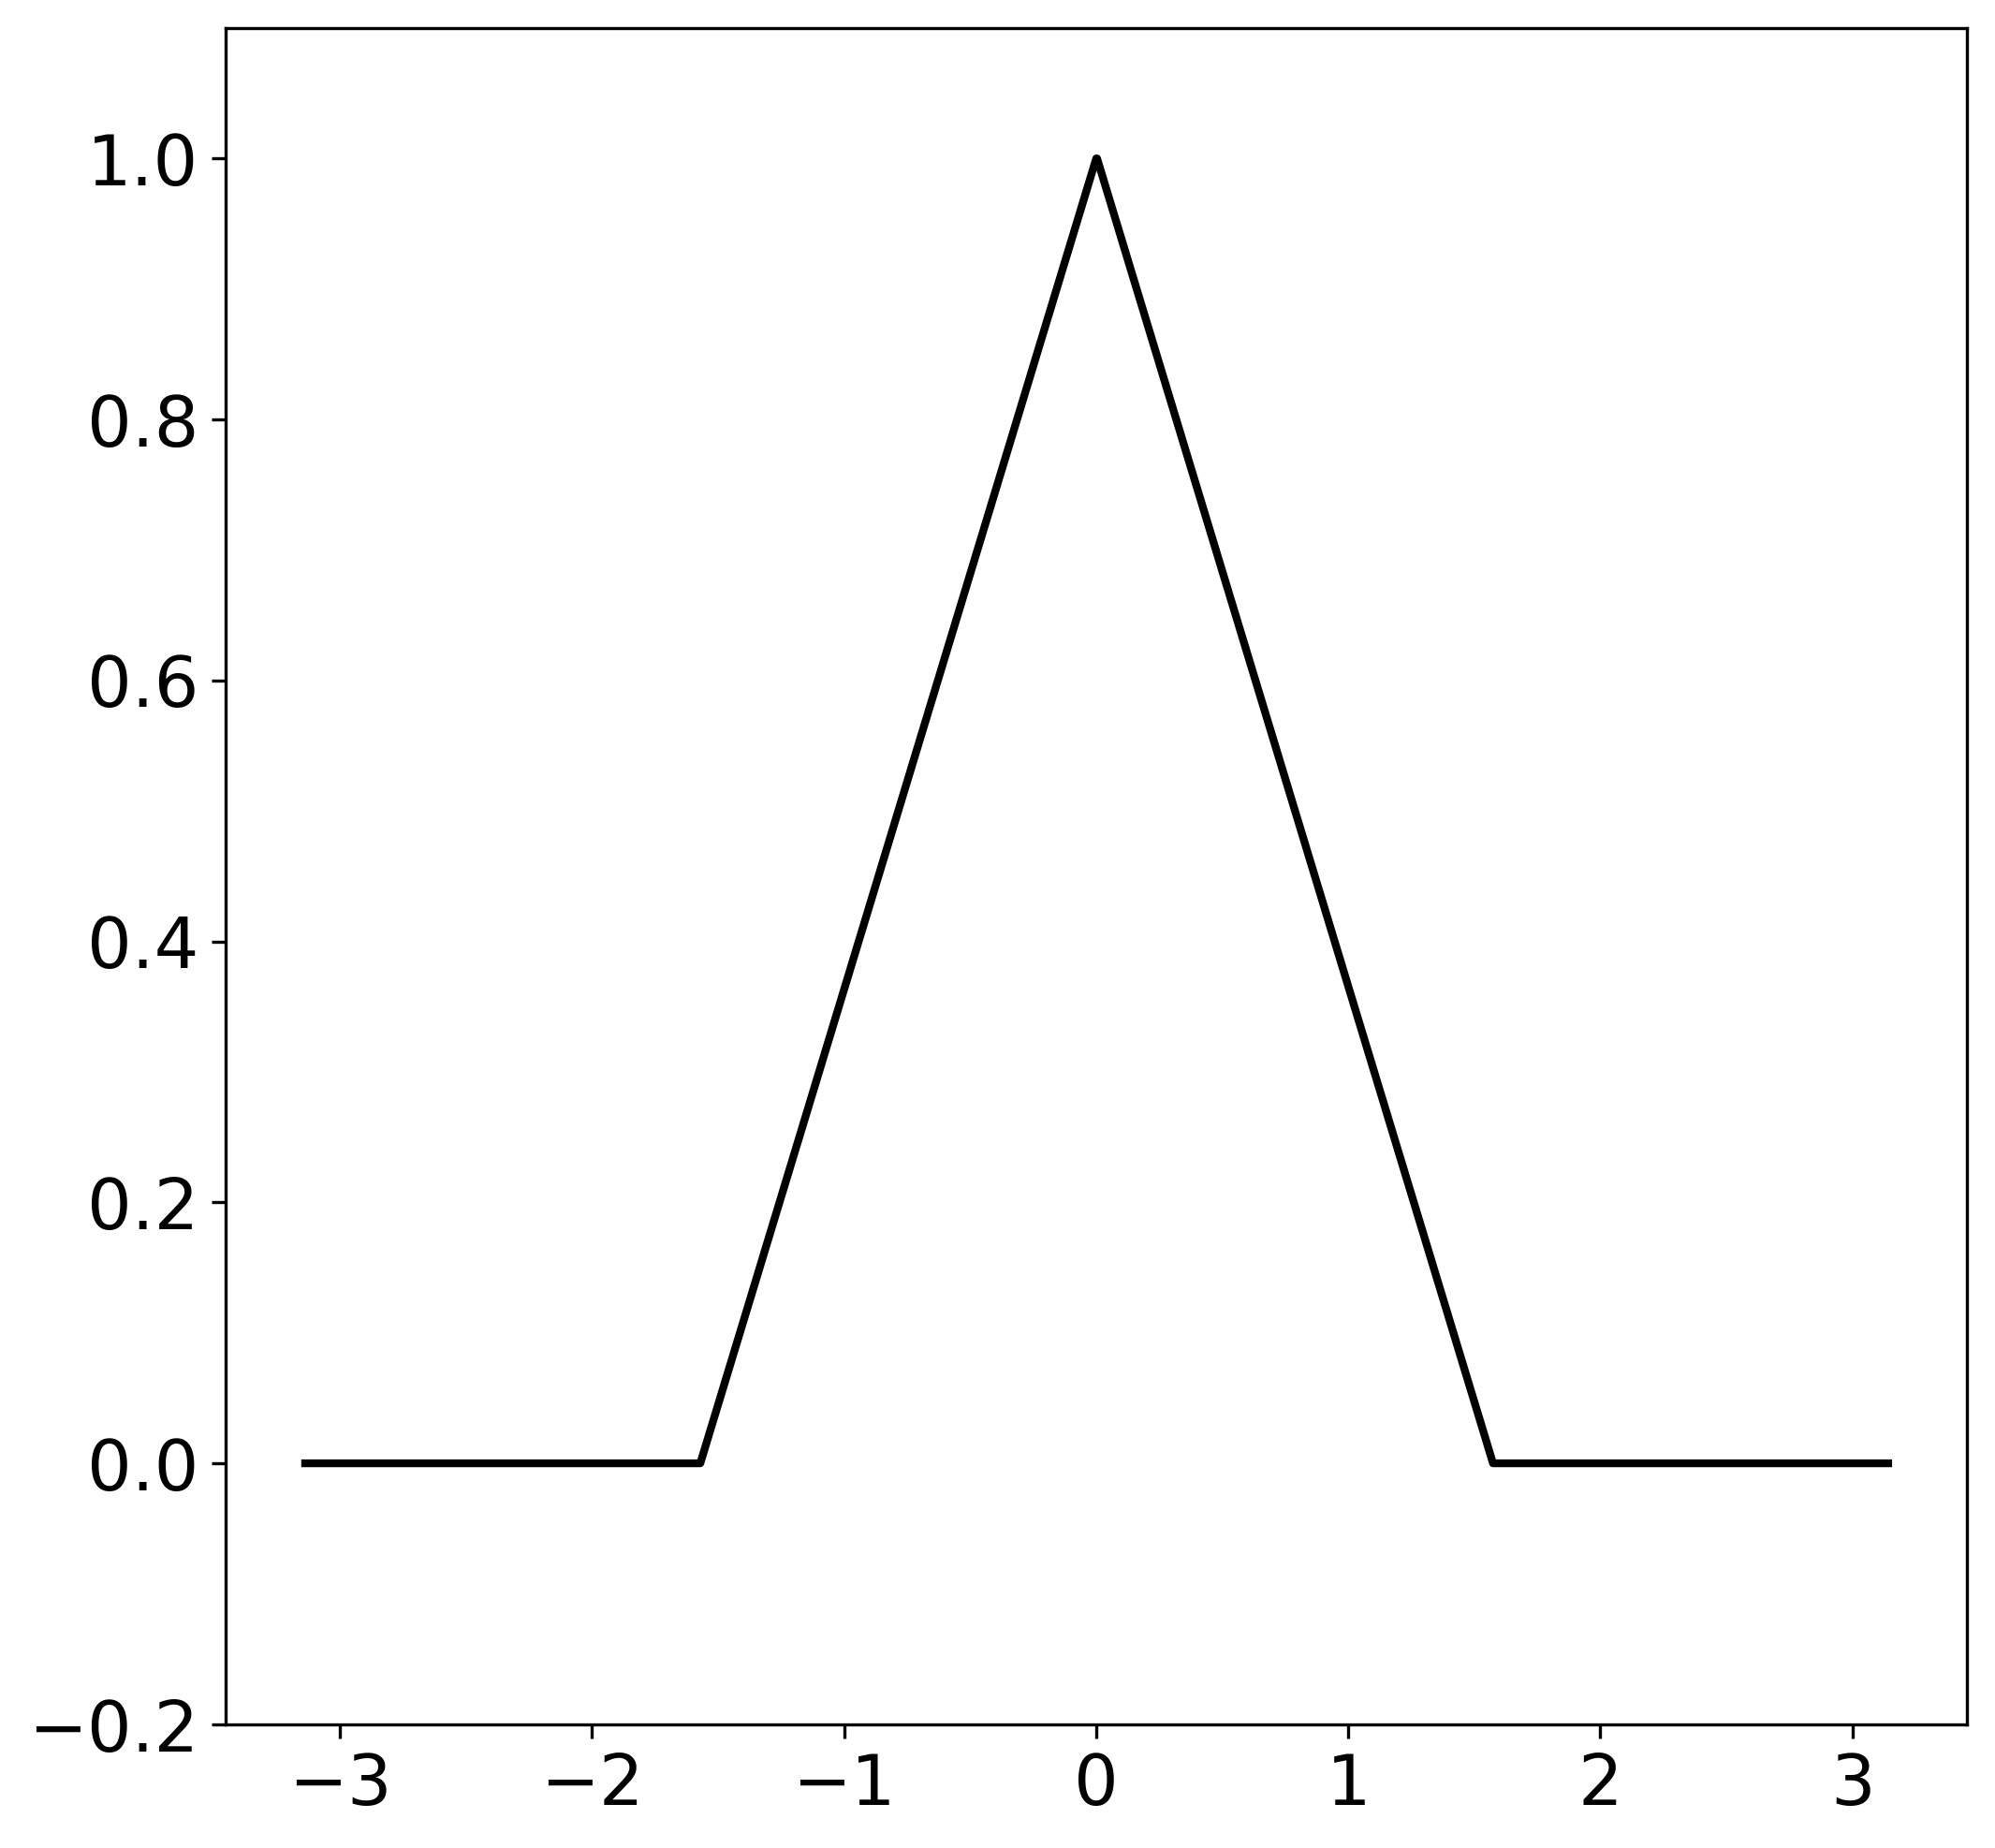
\includegraphics[width=.5\linewidth]{programs/fourier1/out_0.png}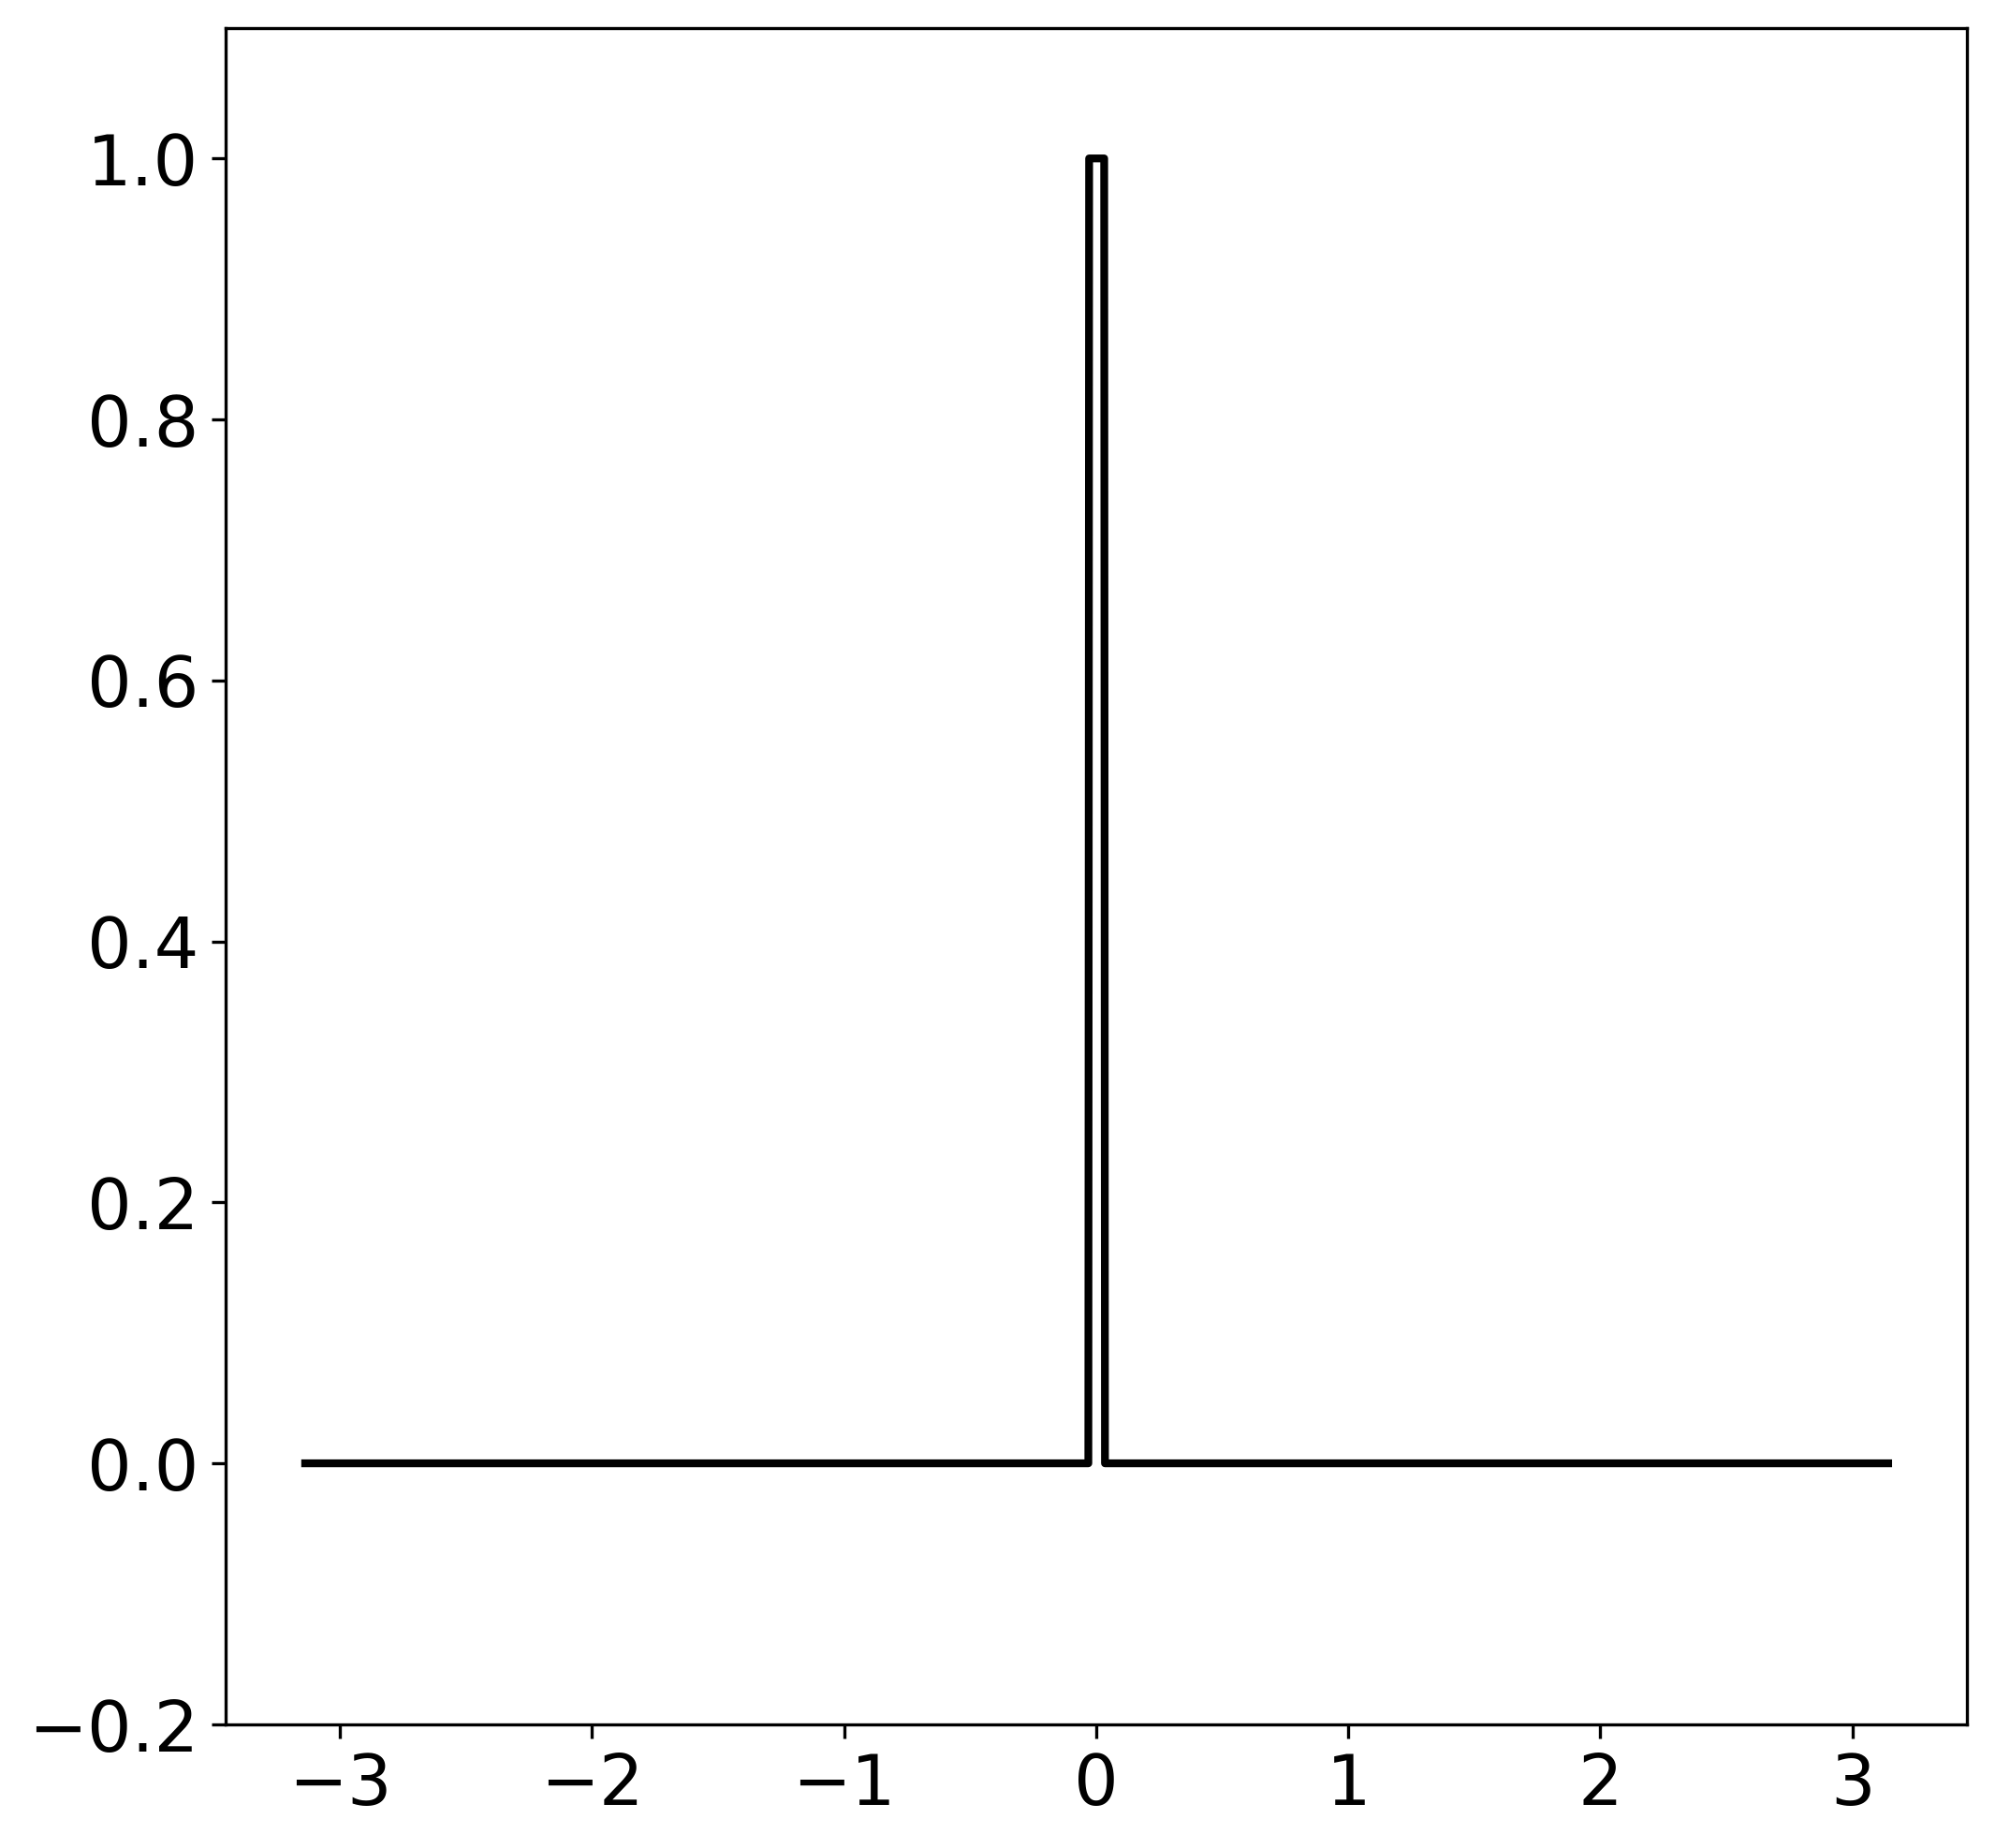
\includegraphics[width=.5\linewidth]{programs/fourier2/out_0.png}}
    \only<2|handout:0>{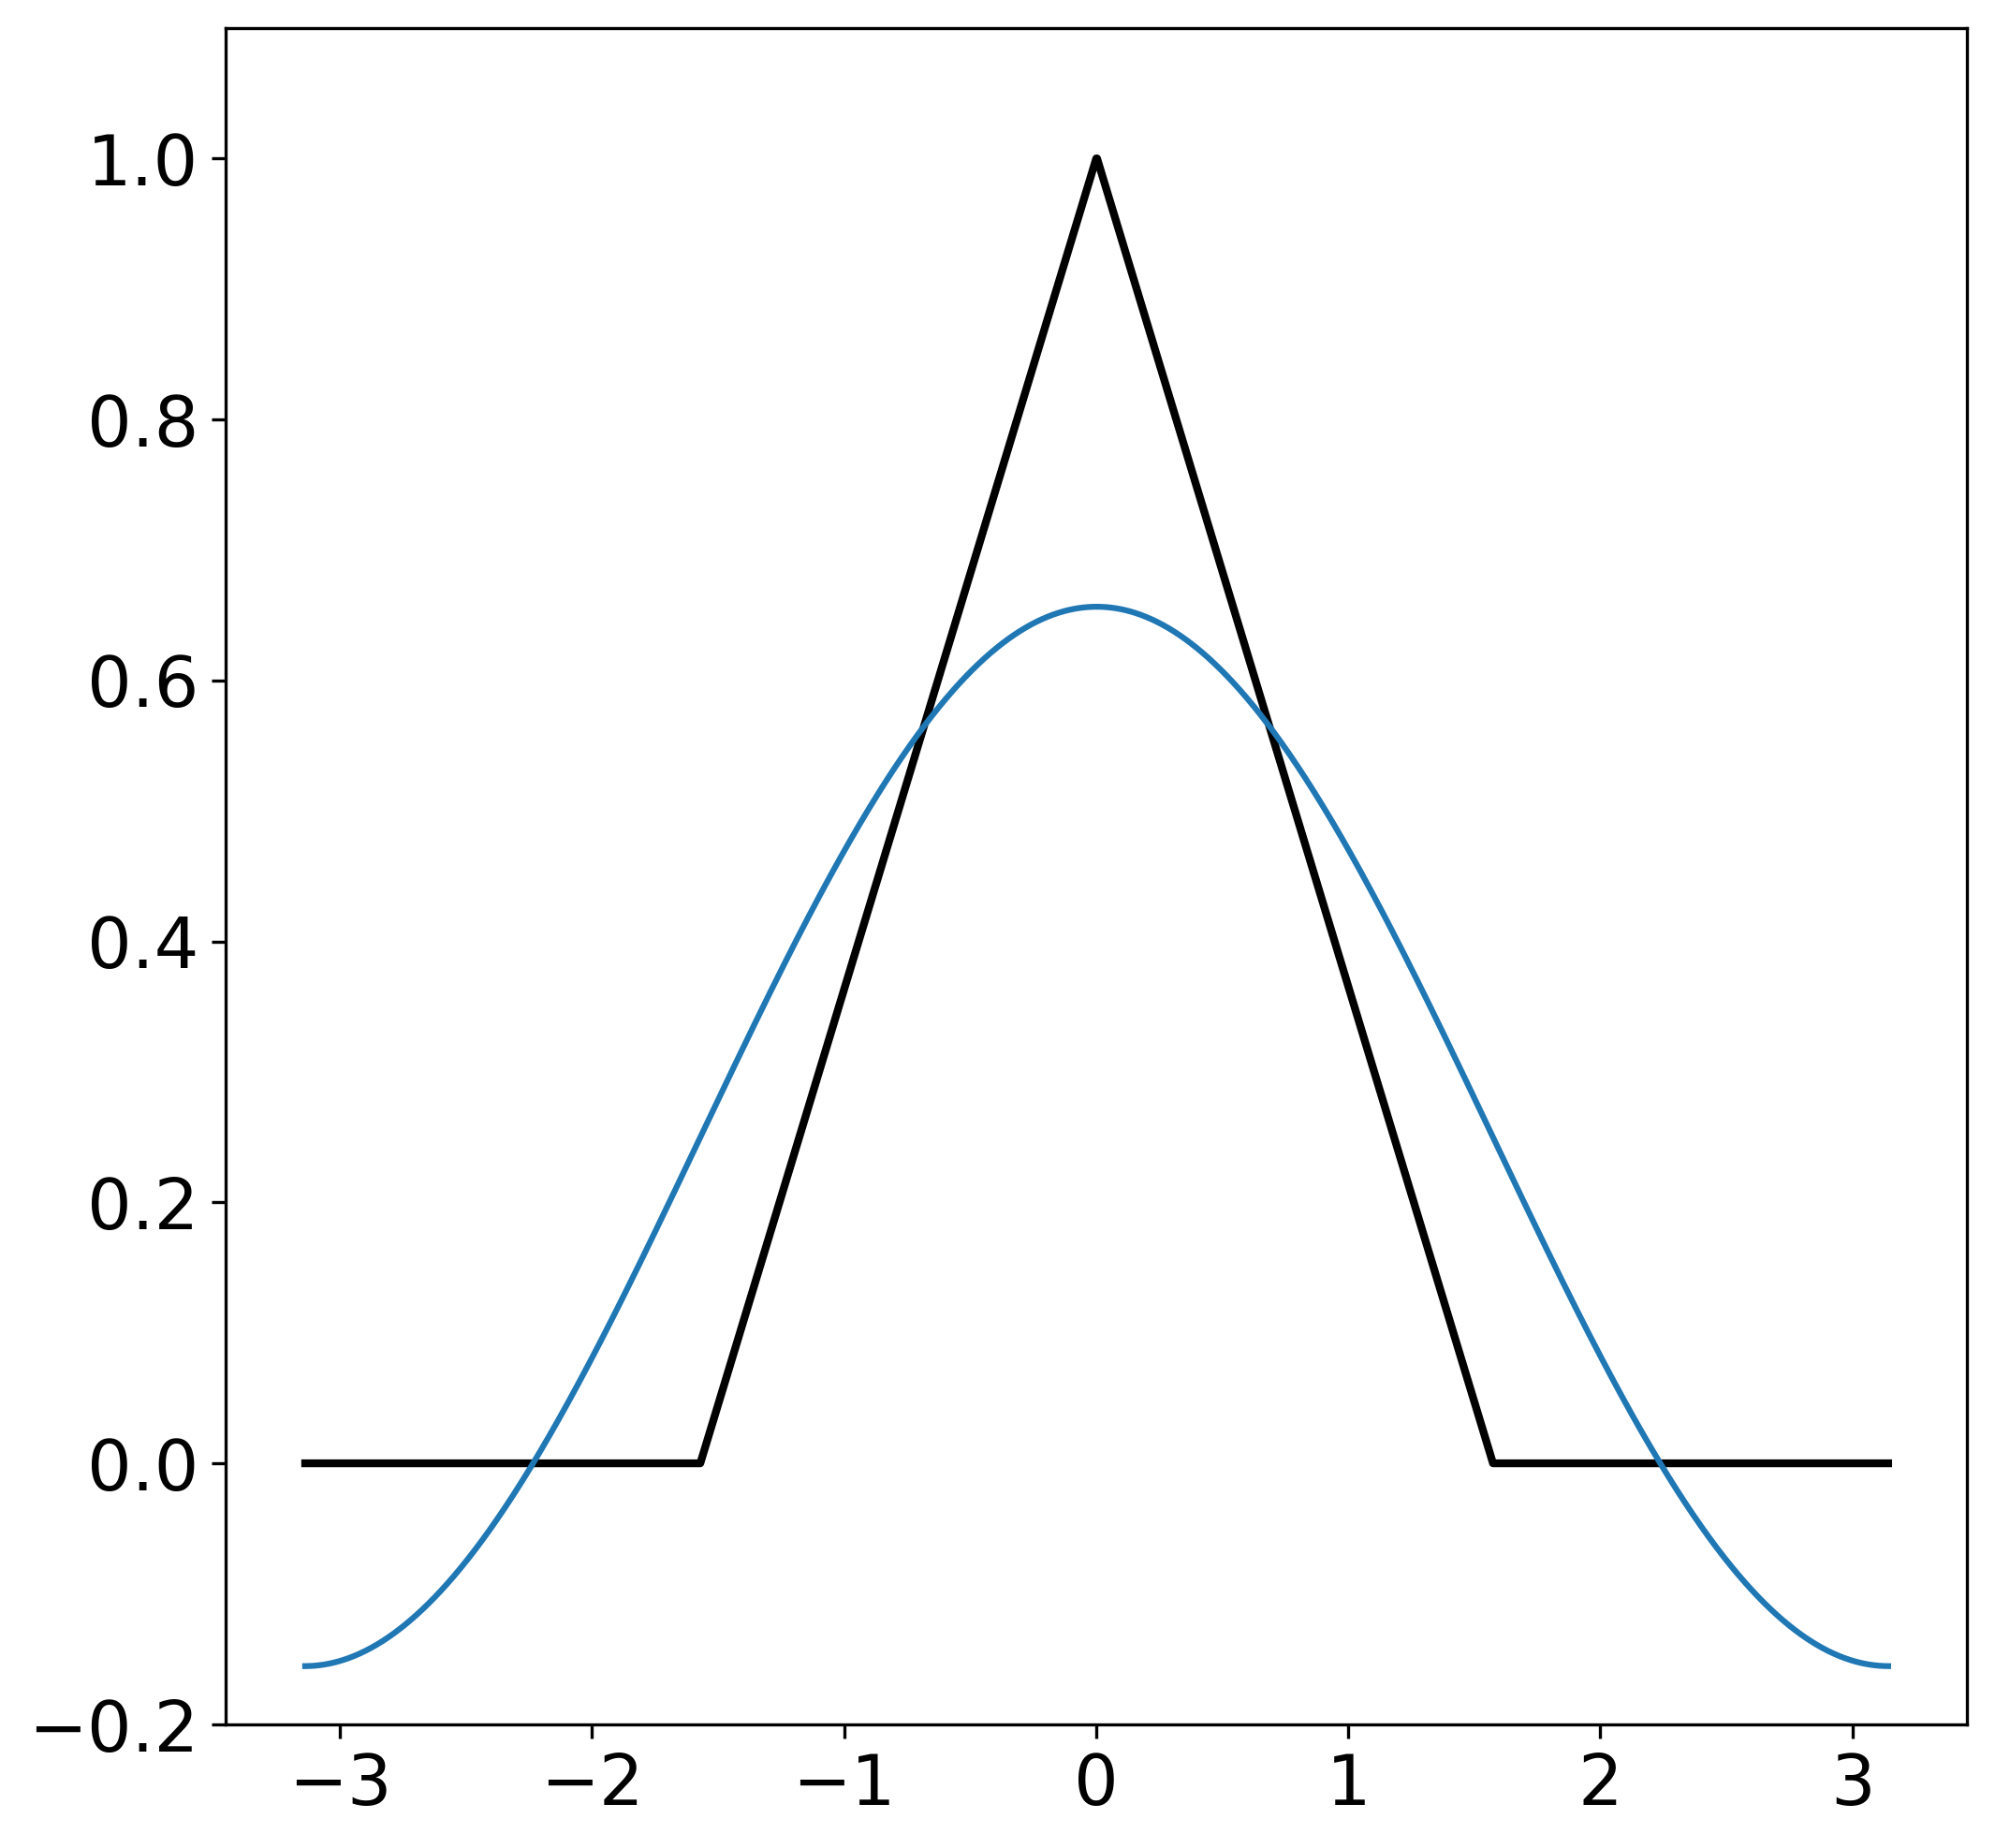
\includegraphics[width=.5\linewidth]{programs/fourier1/out_1.png}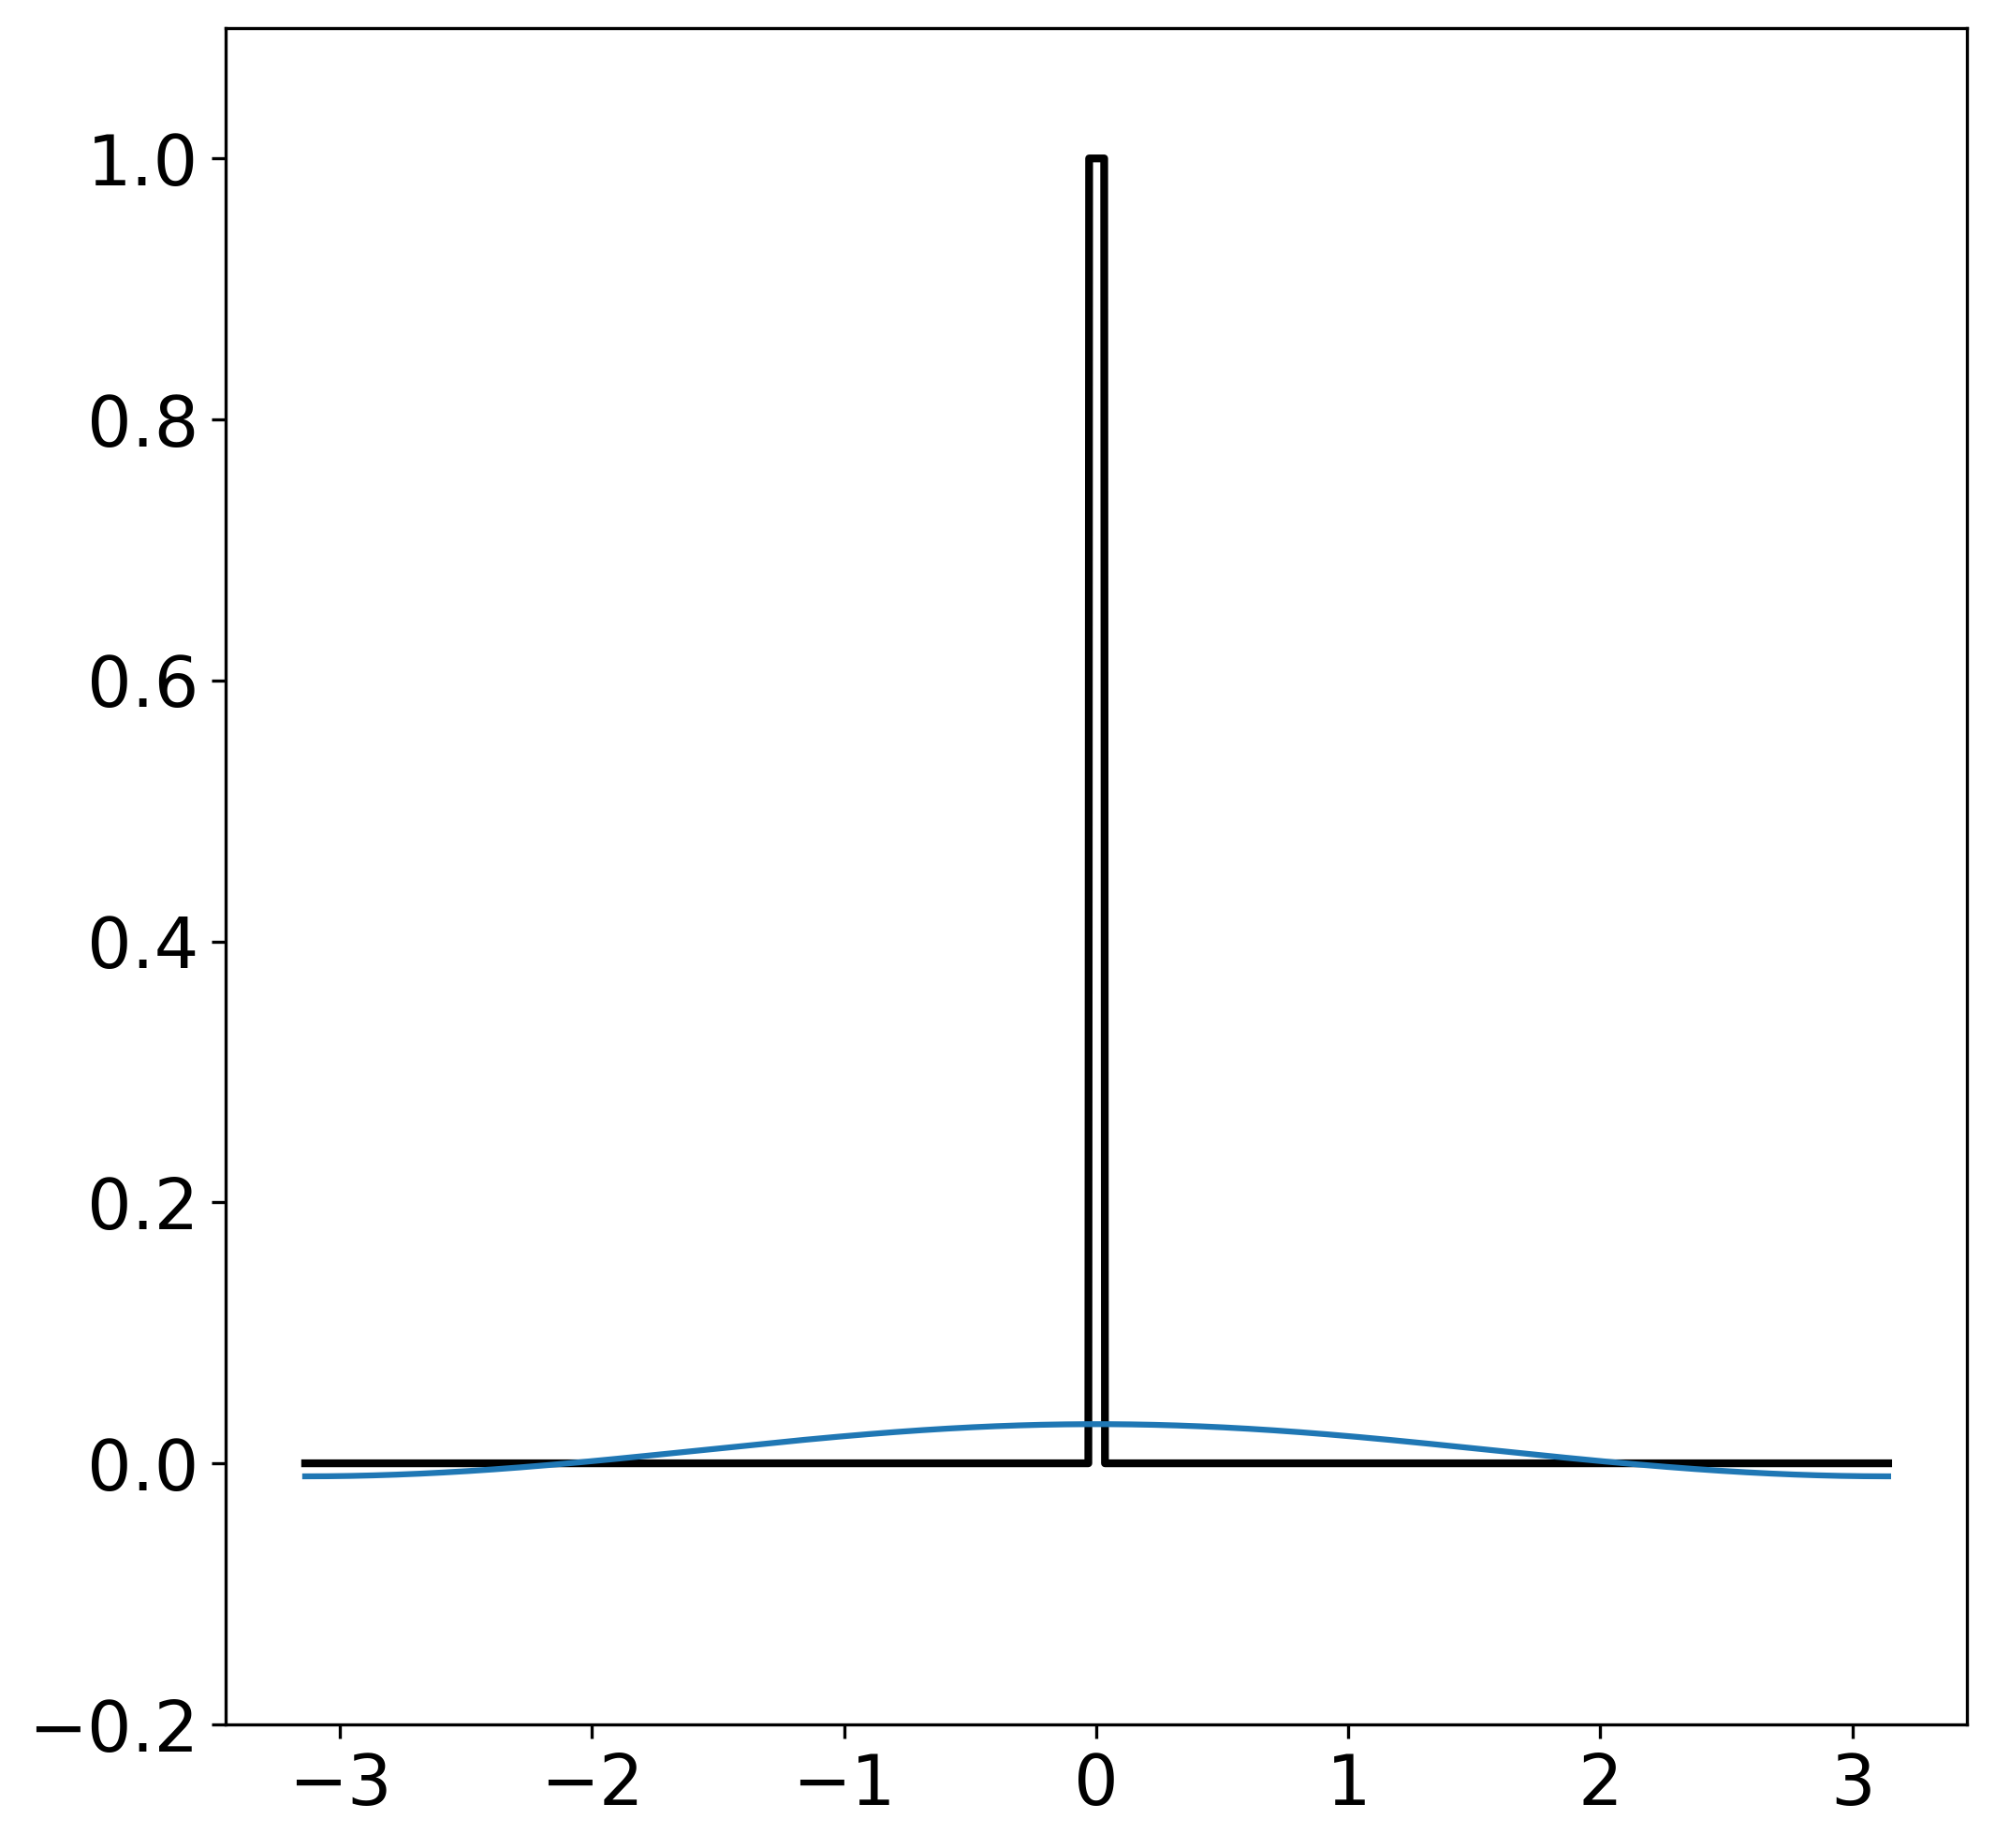
\includegraphics[width=.5\linewidth]{programs/fourier2/out_1.png}}
    \only<3|handout:0>{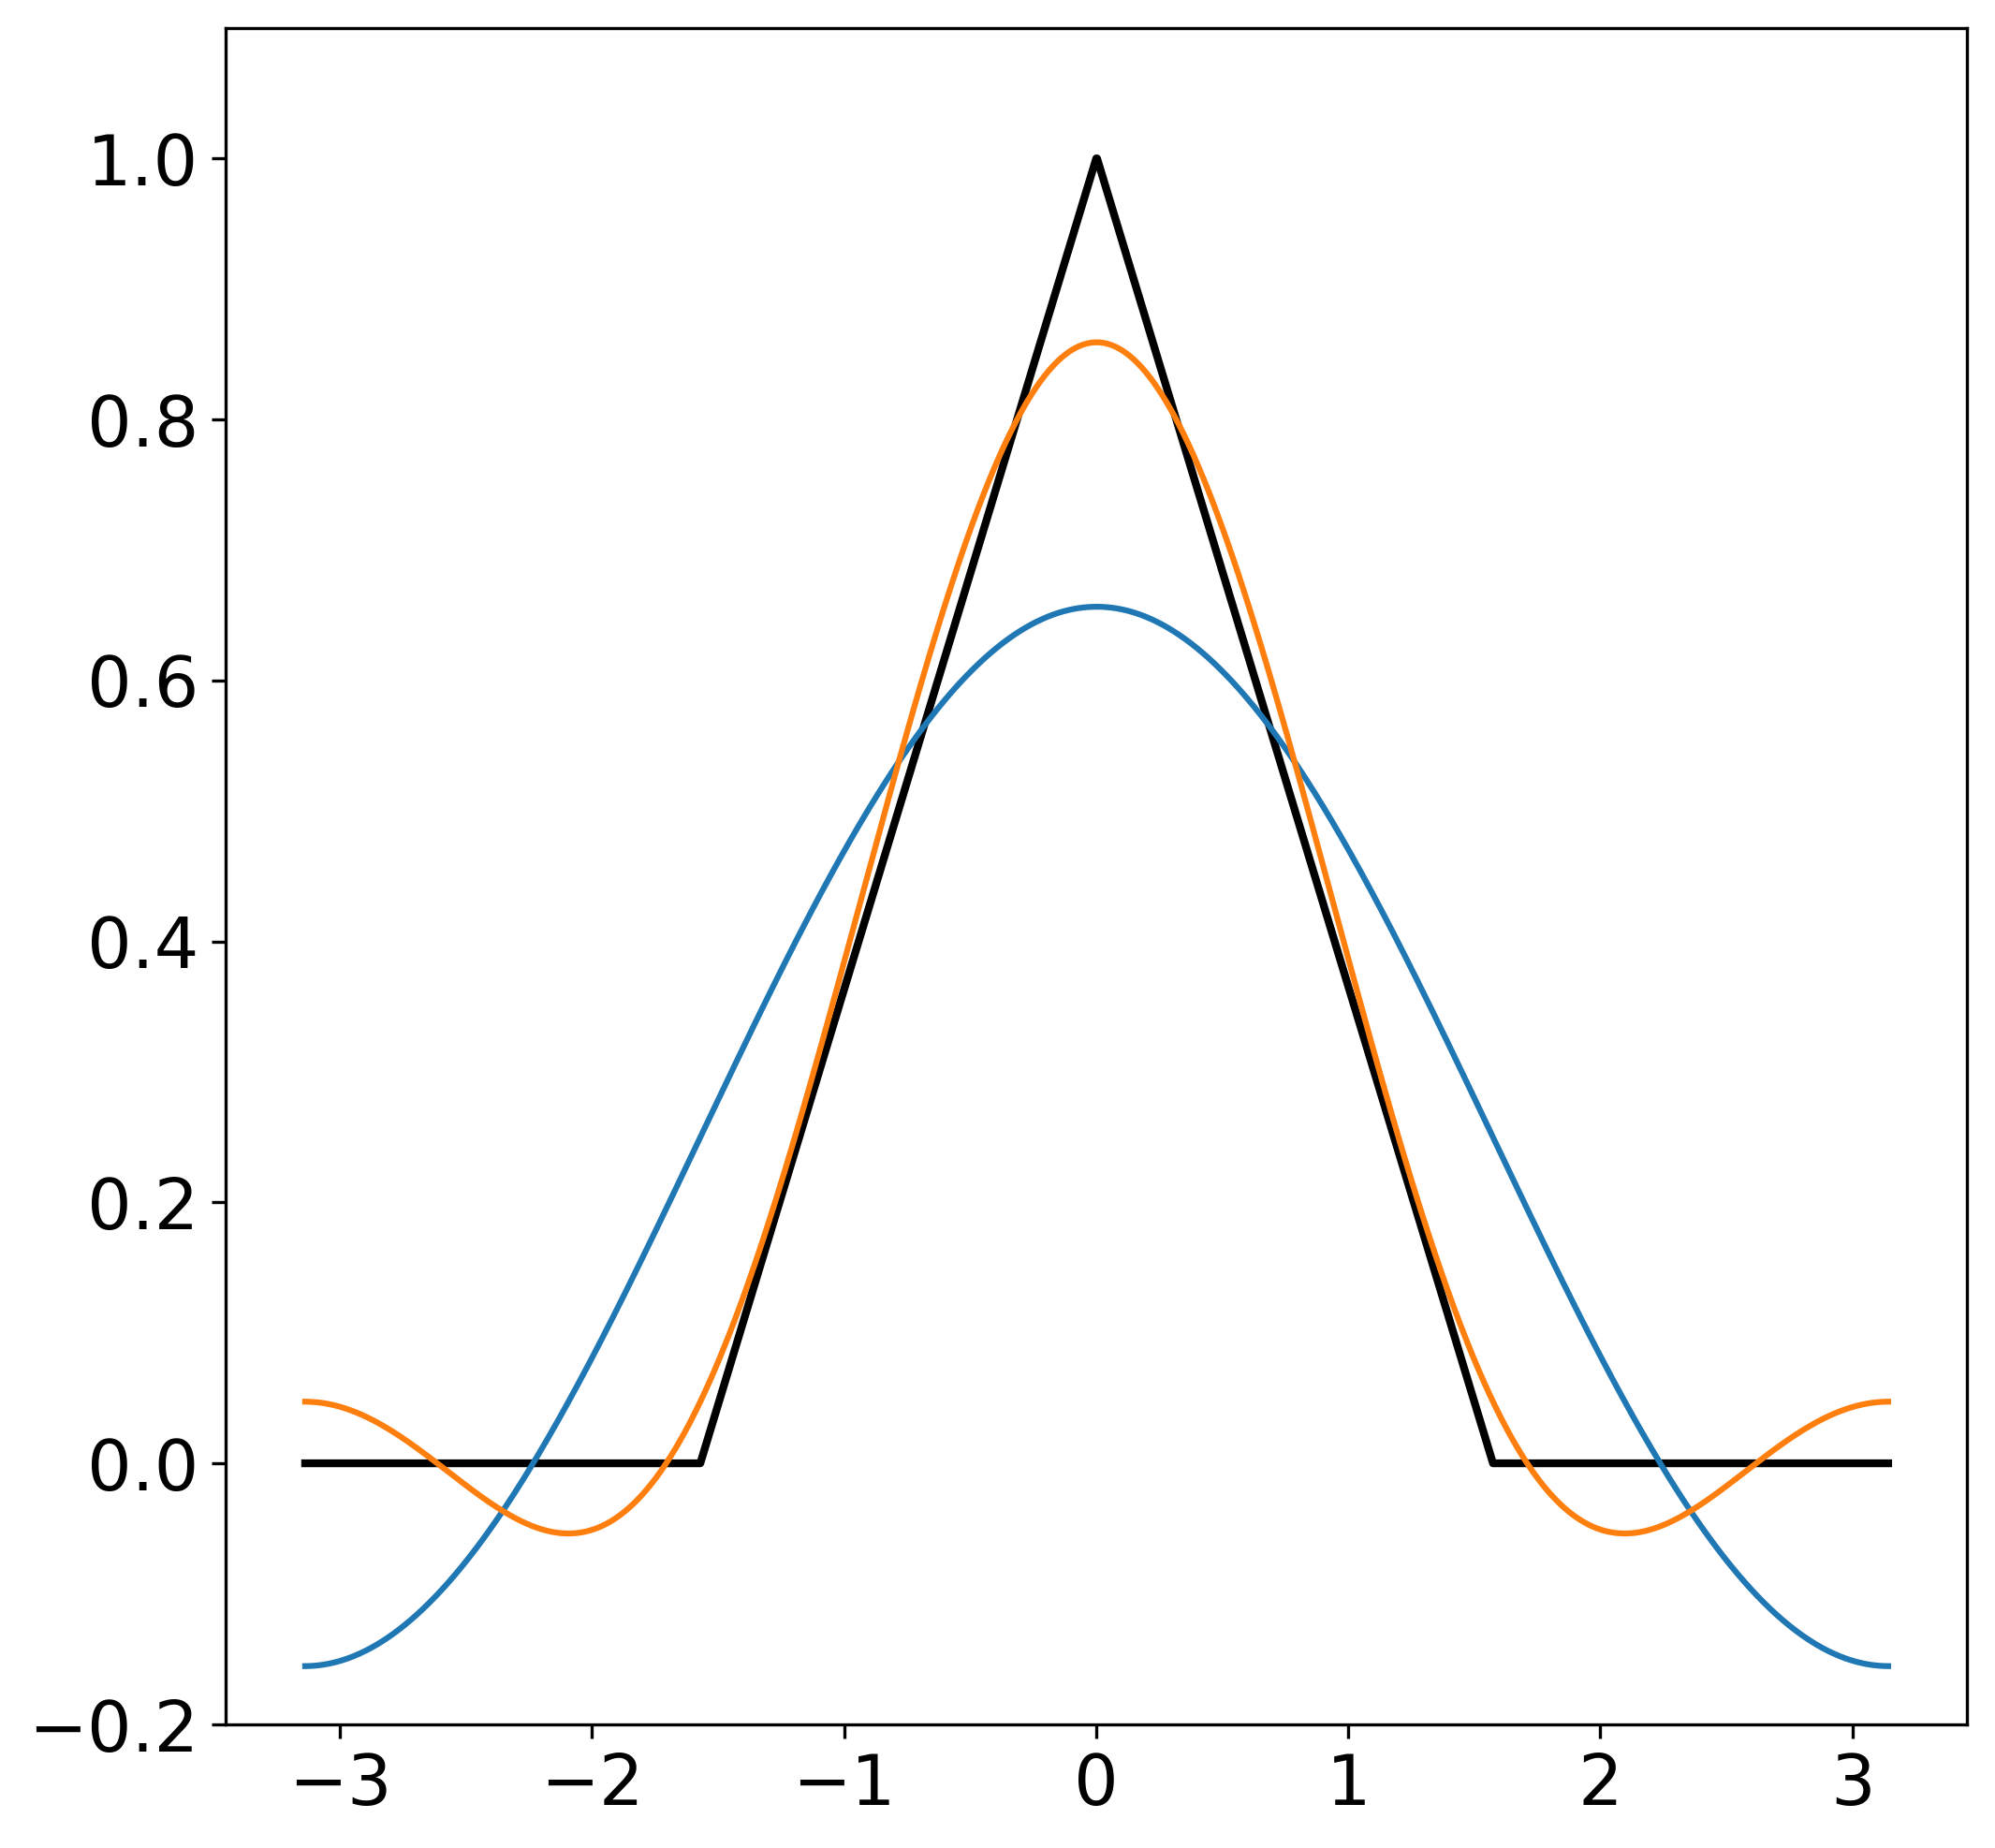
\includegraphics[width=.5\linewidth]{programs/fourier1/out_2.png}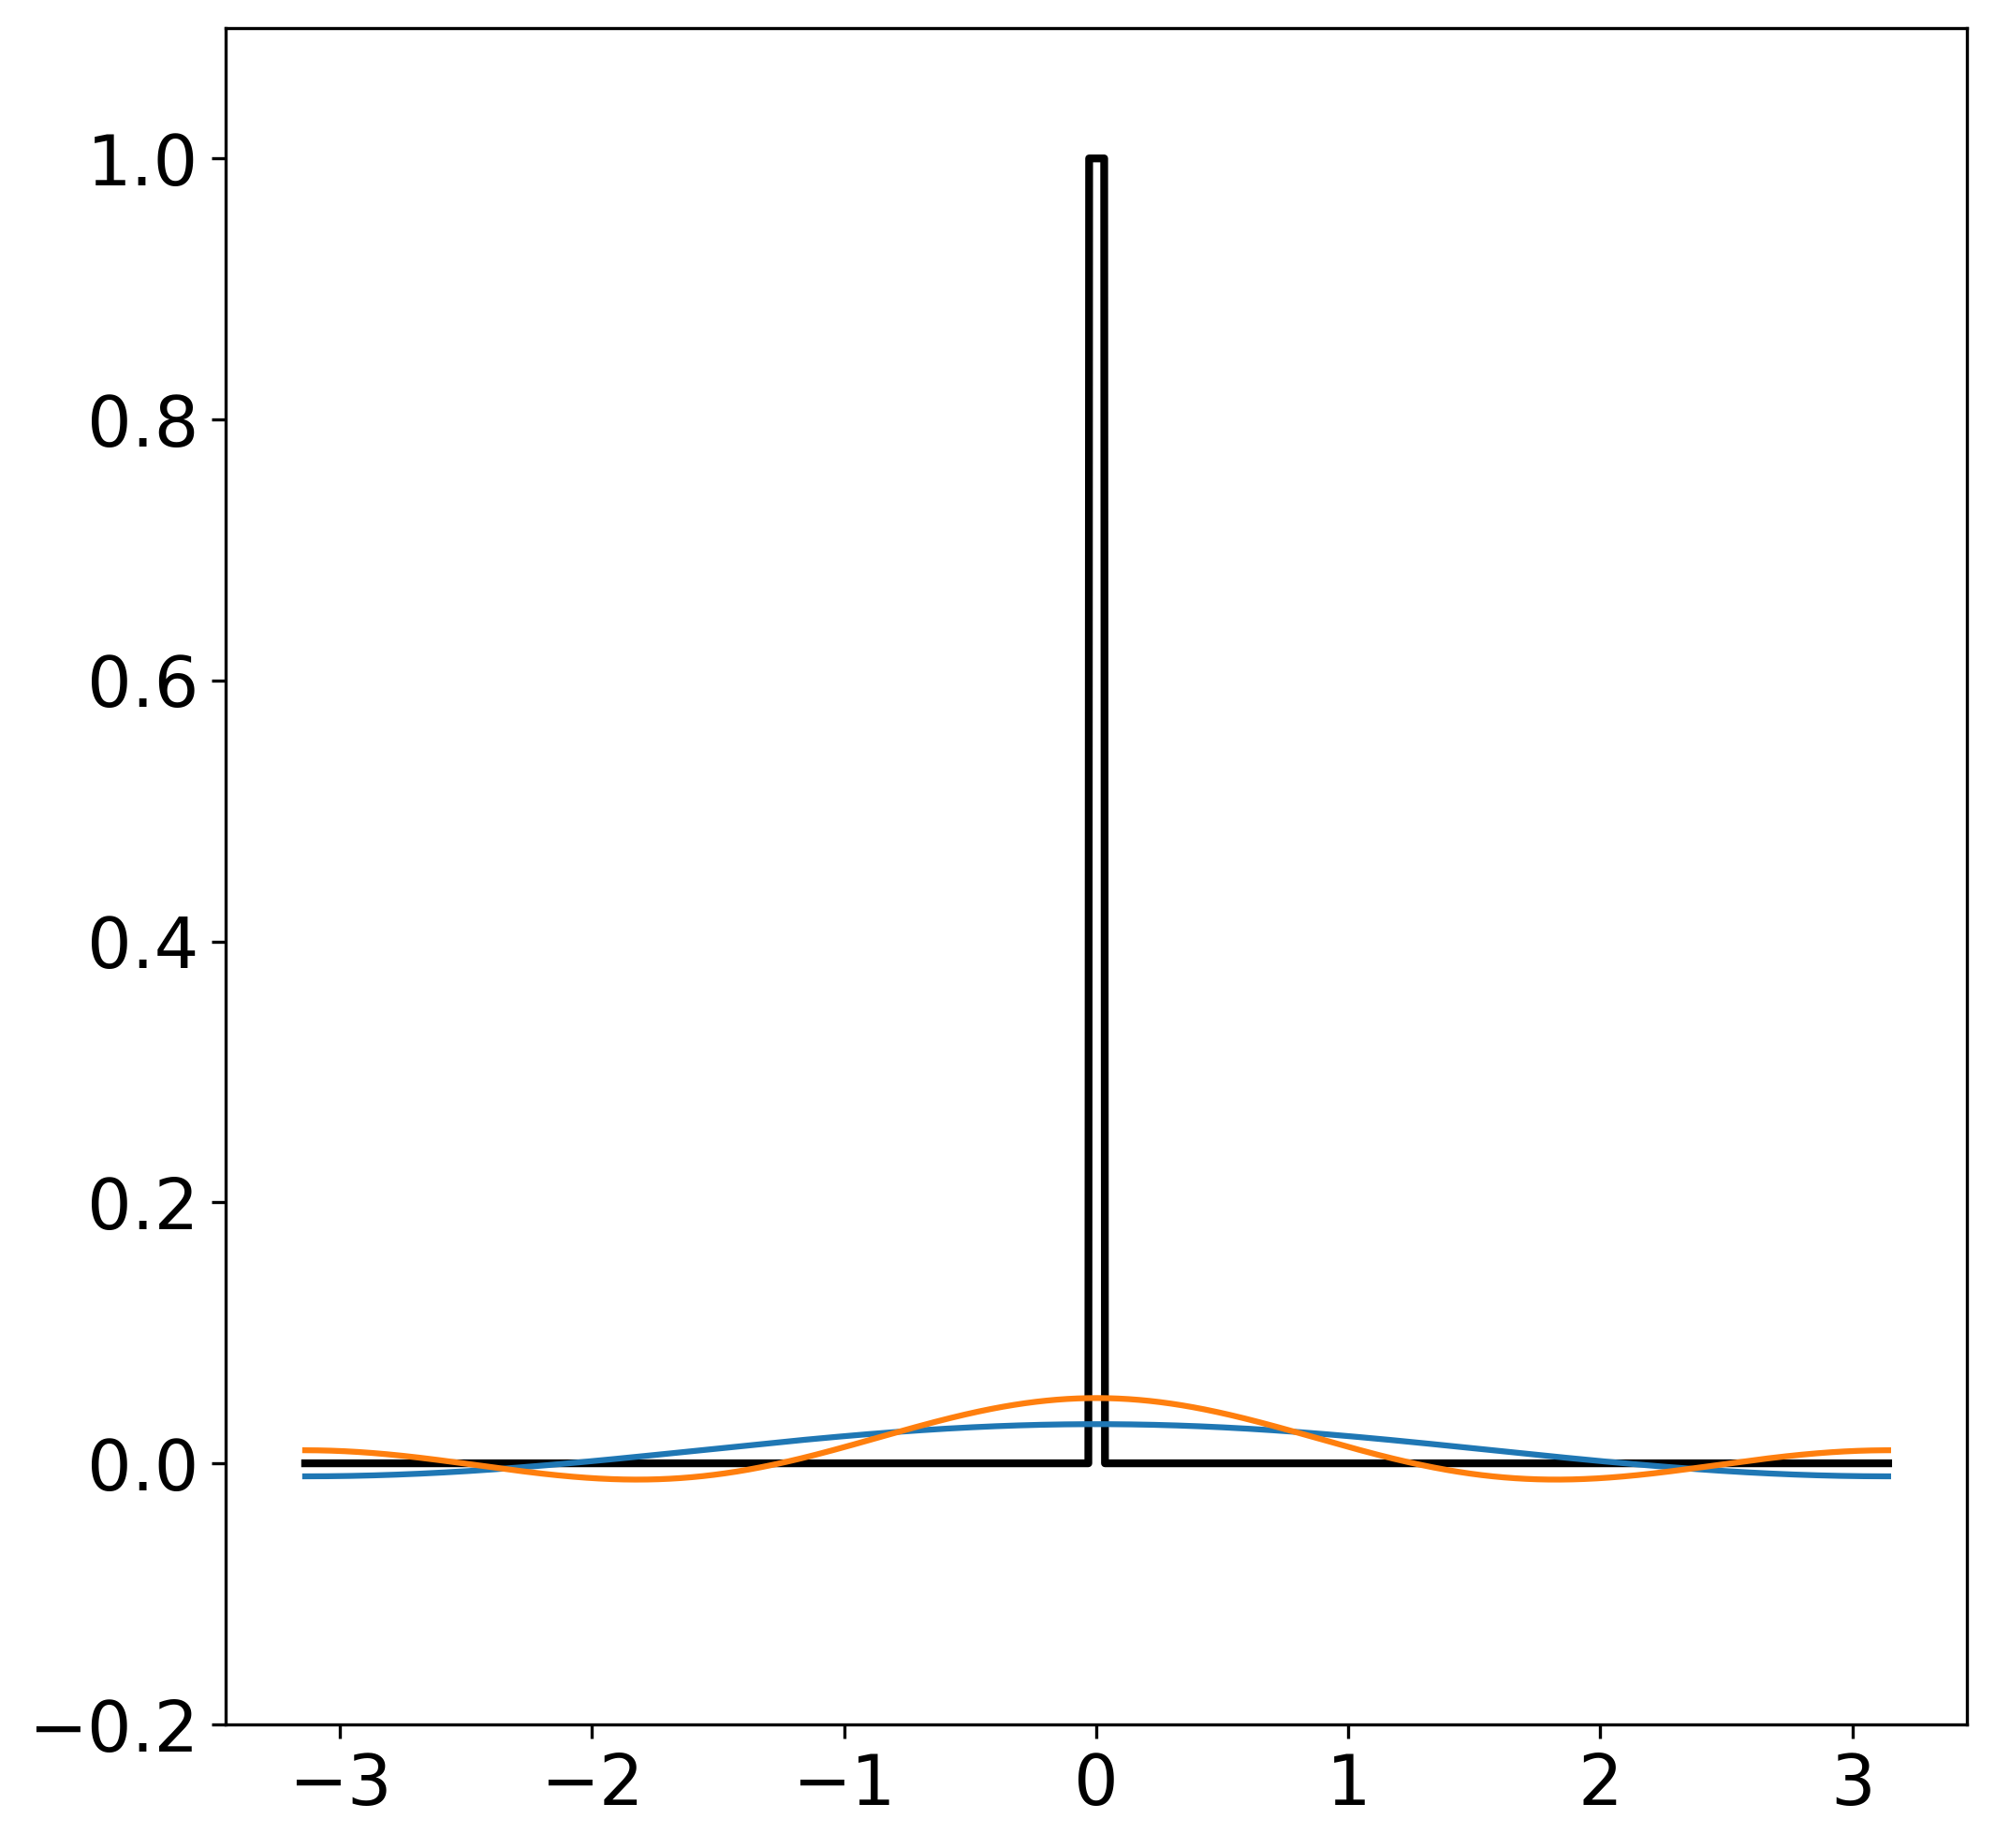
\includegraphics[width=.5\linewidth]{programs/fourier2/out_2.png}}
    \only<4|handout:0>{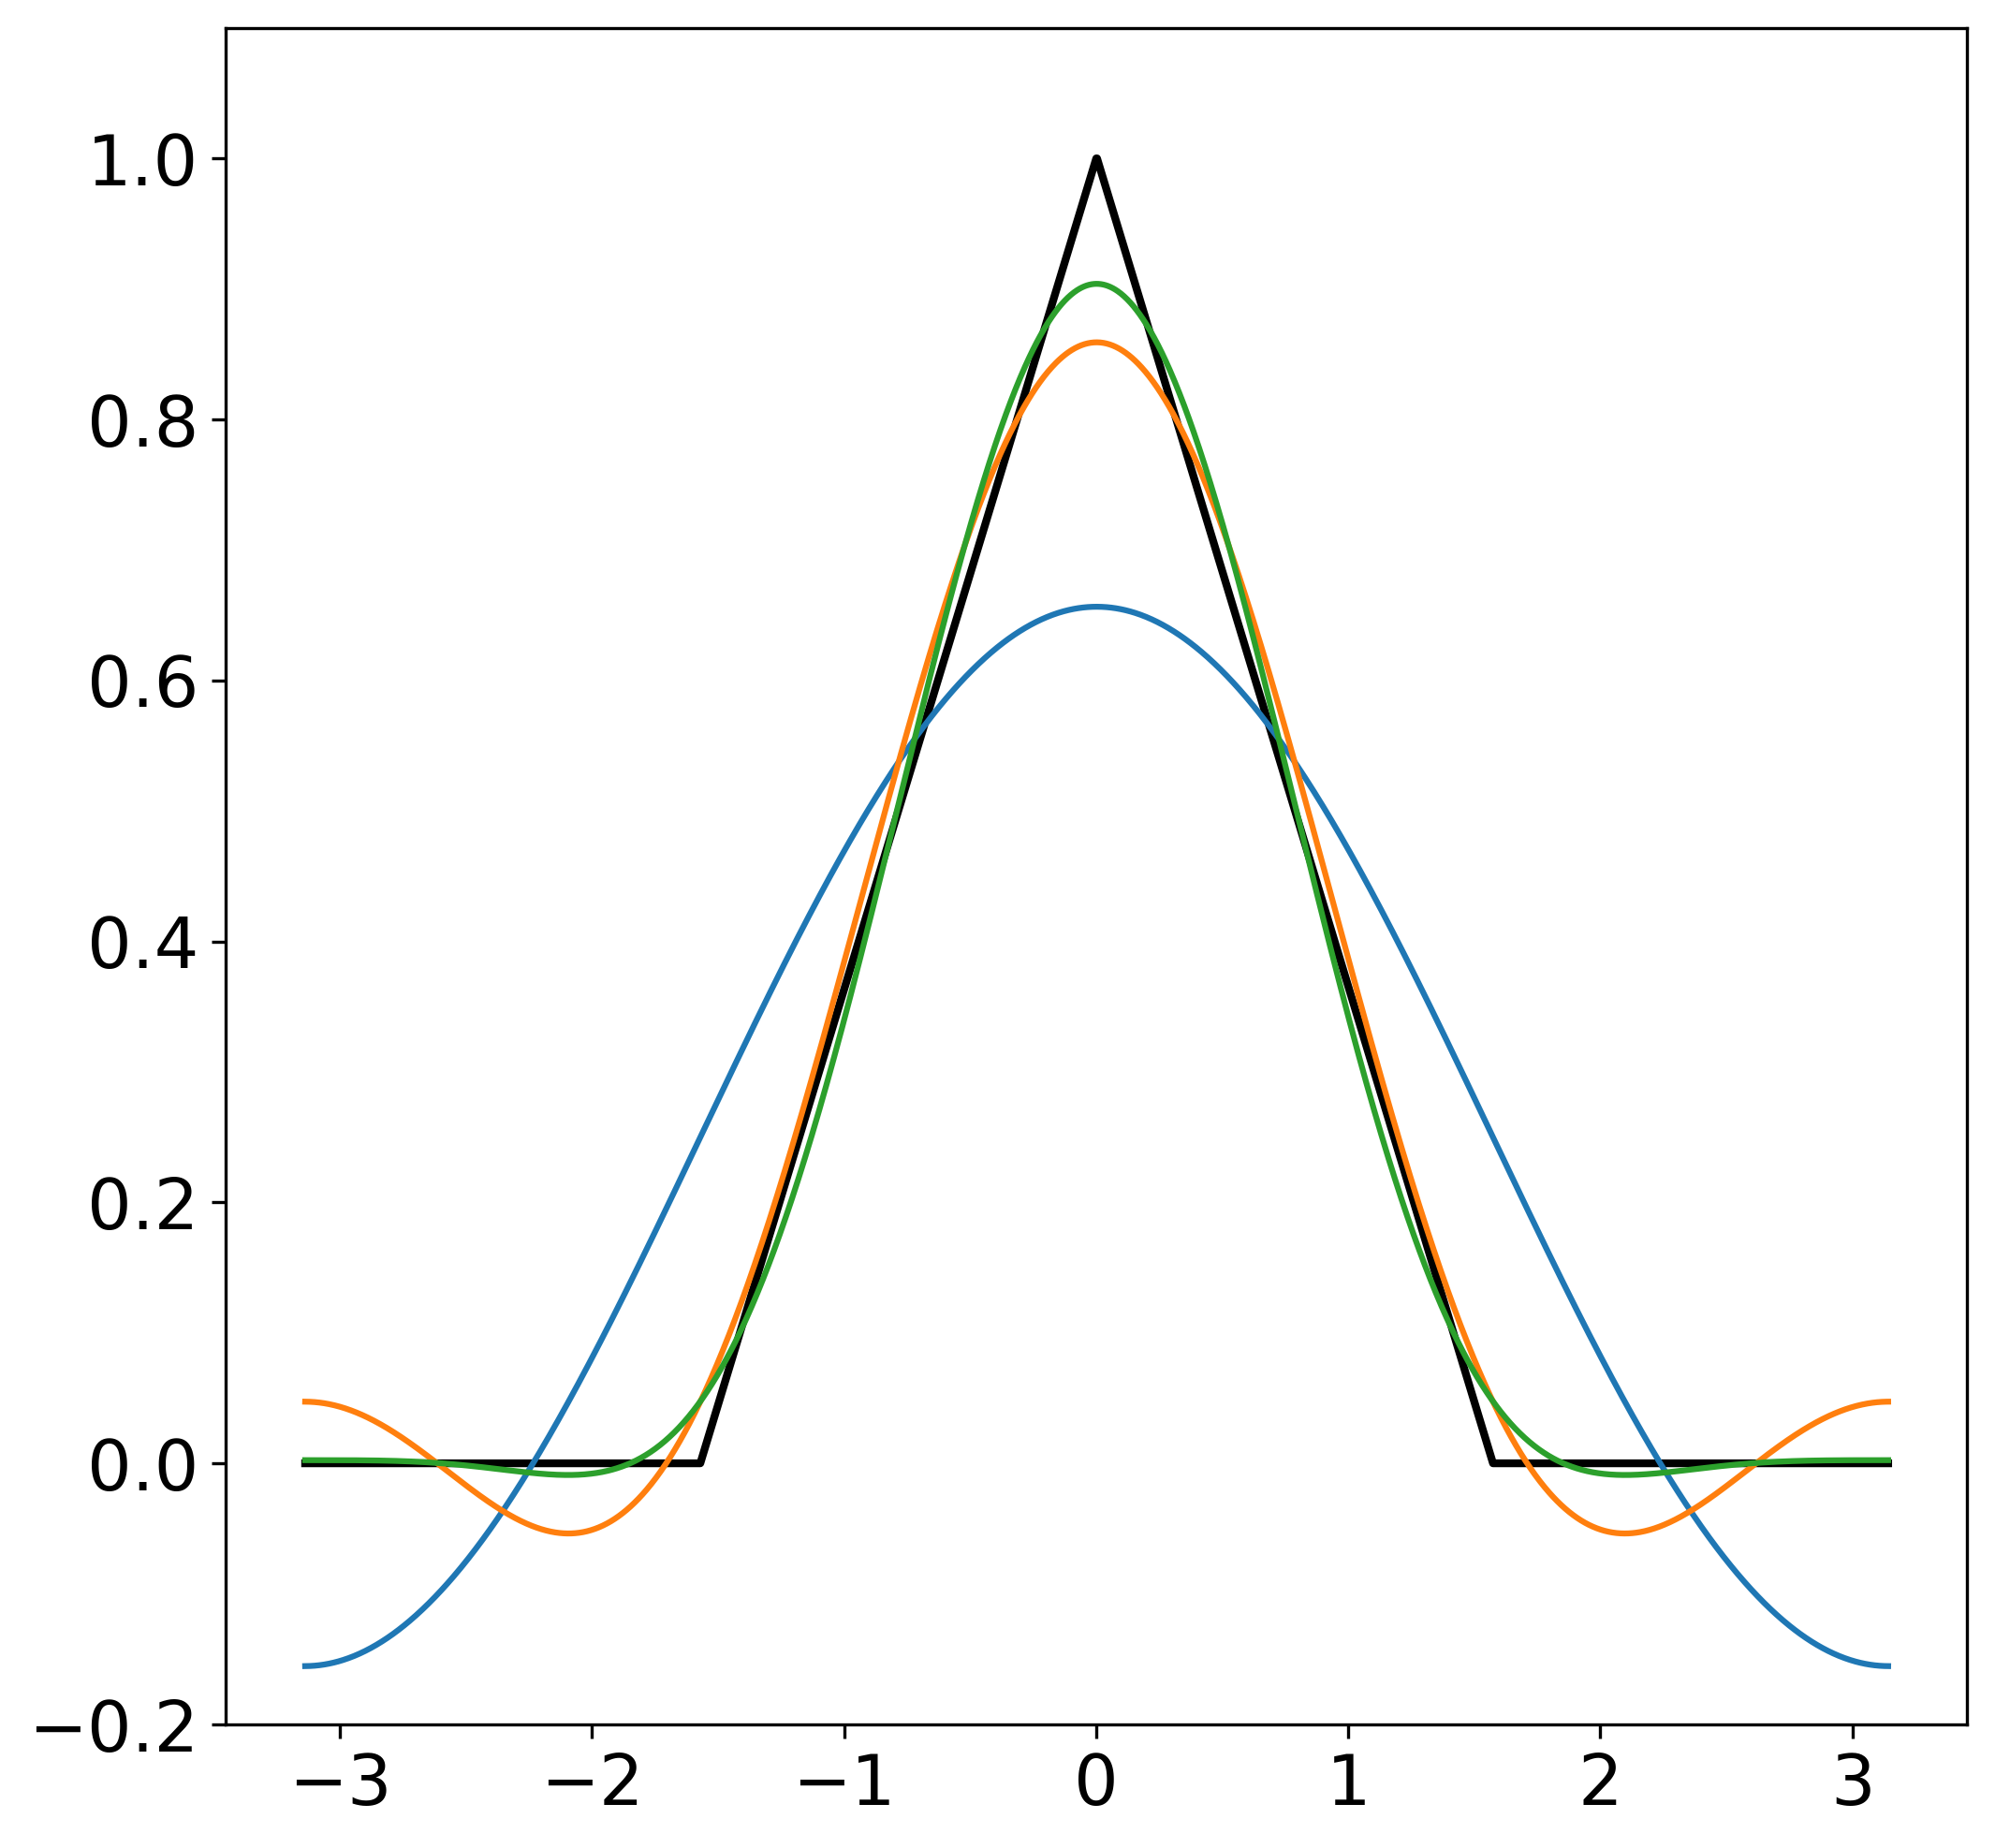
\includegraphics[width=.5\linewidth]{programs/fourier1/out_3.png}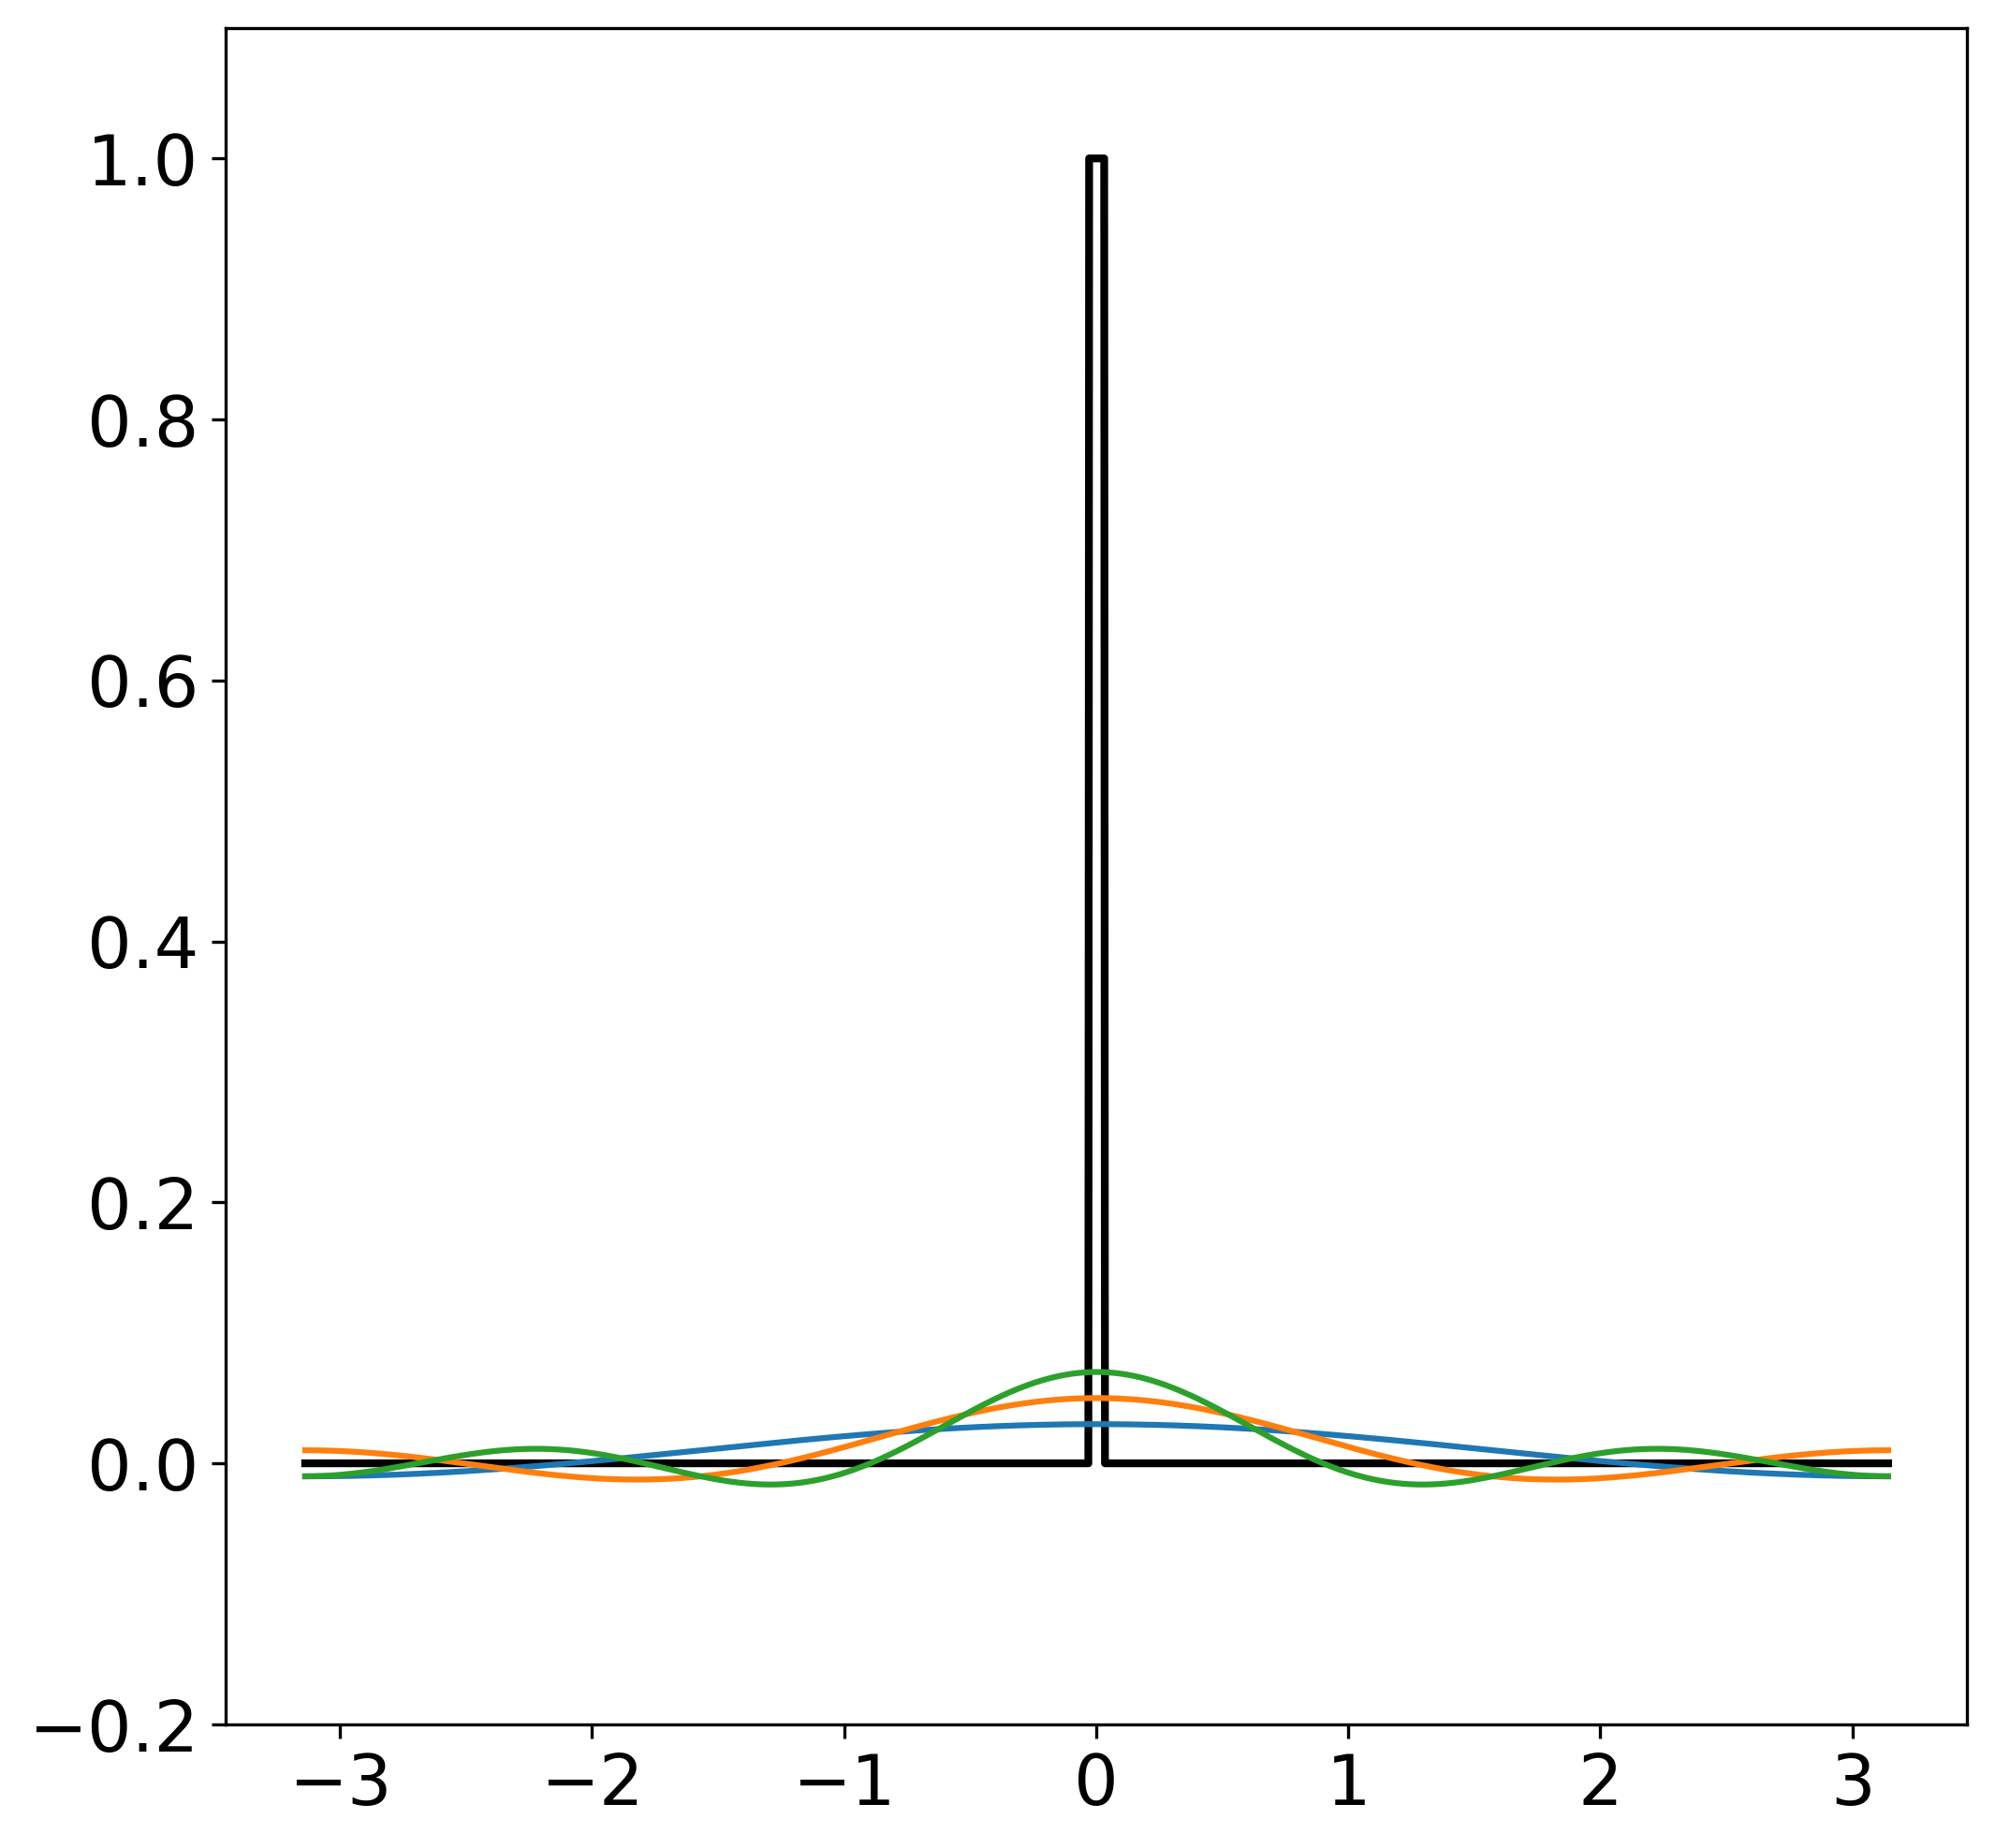
\includegraphics[width=.5\linewidth]{programs/fourier2/out_3.png}}
    \only<5|handout:0>{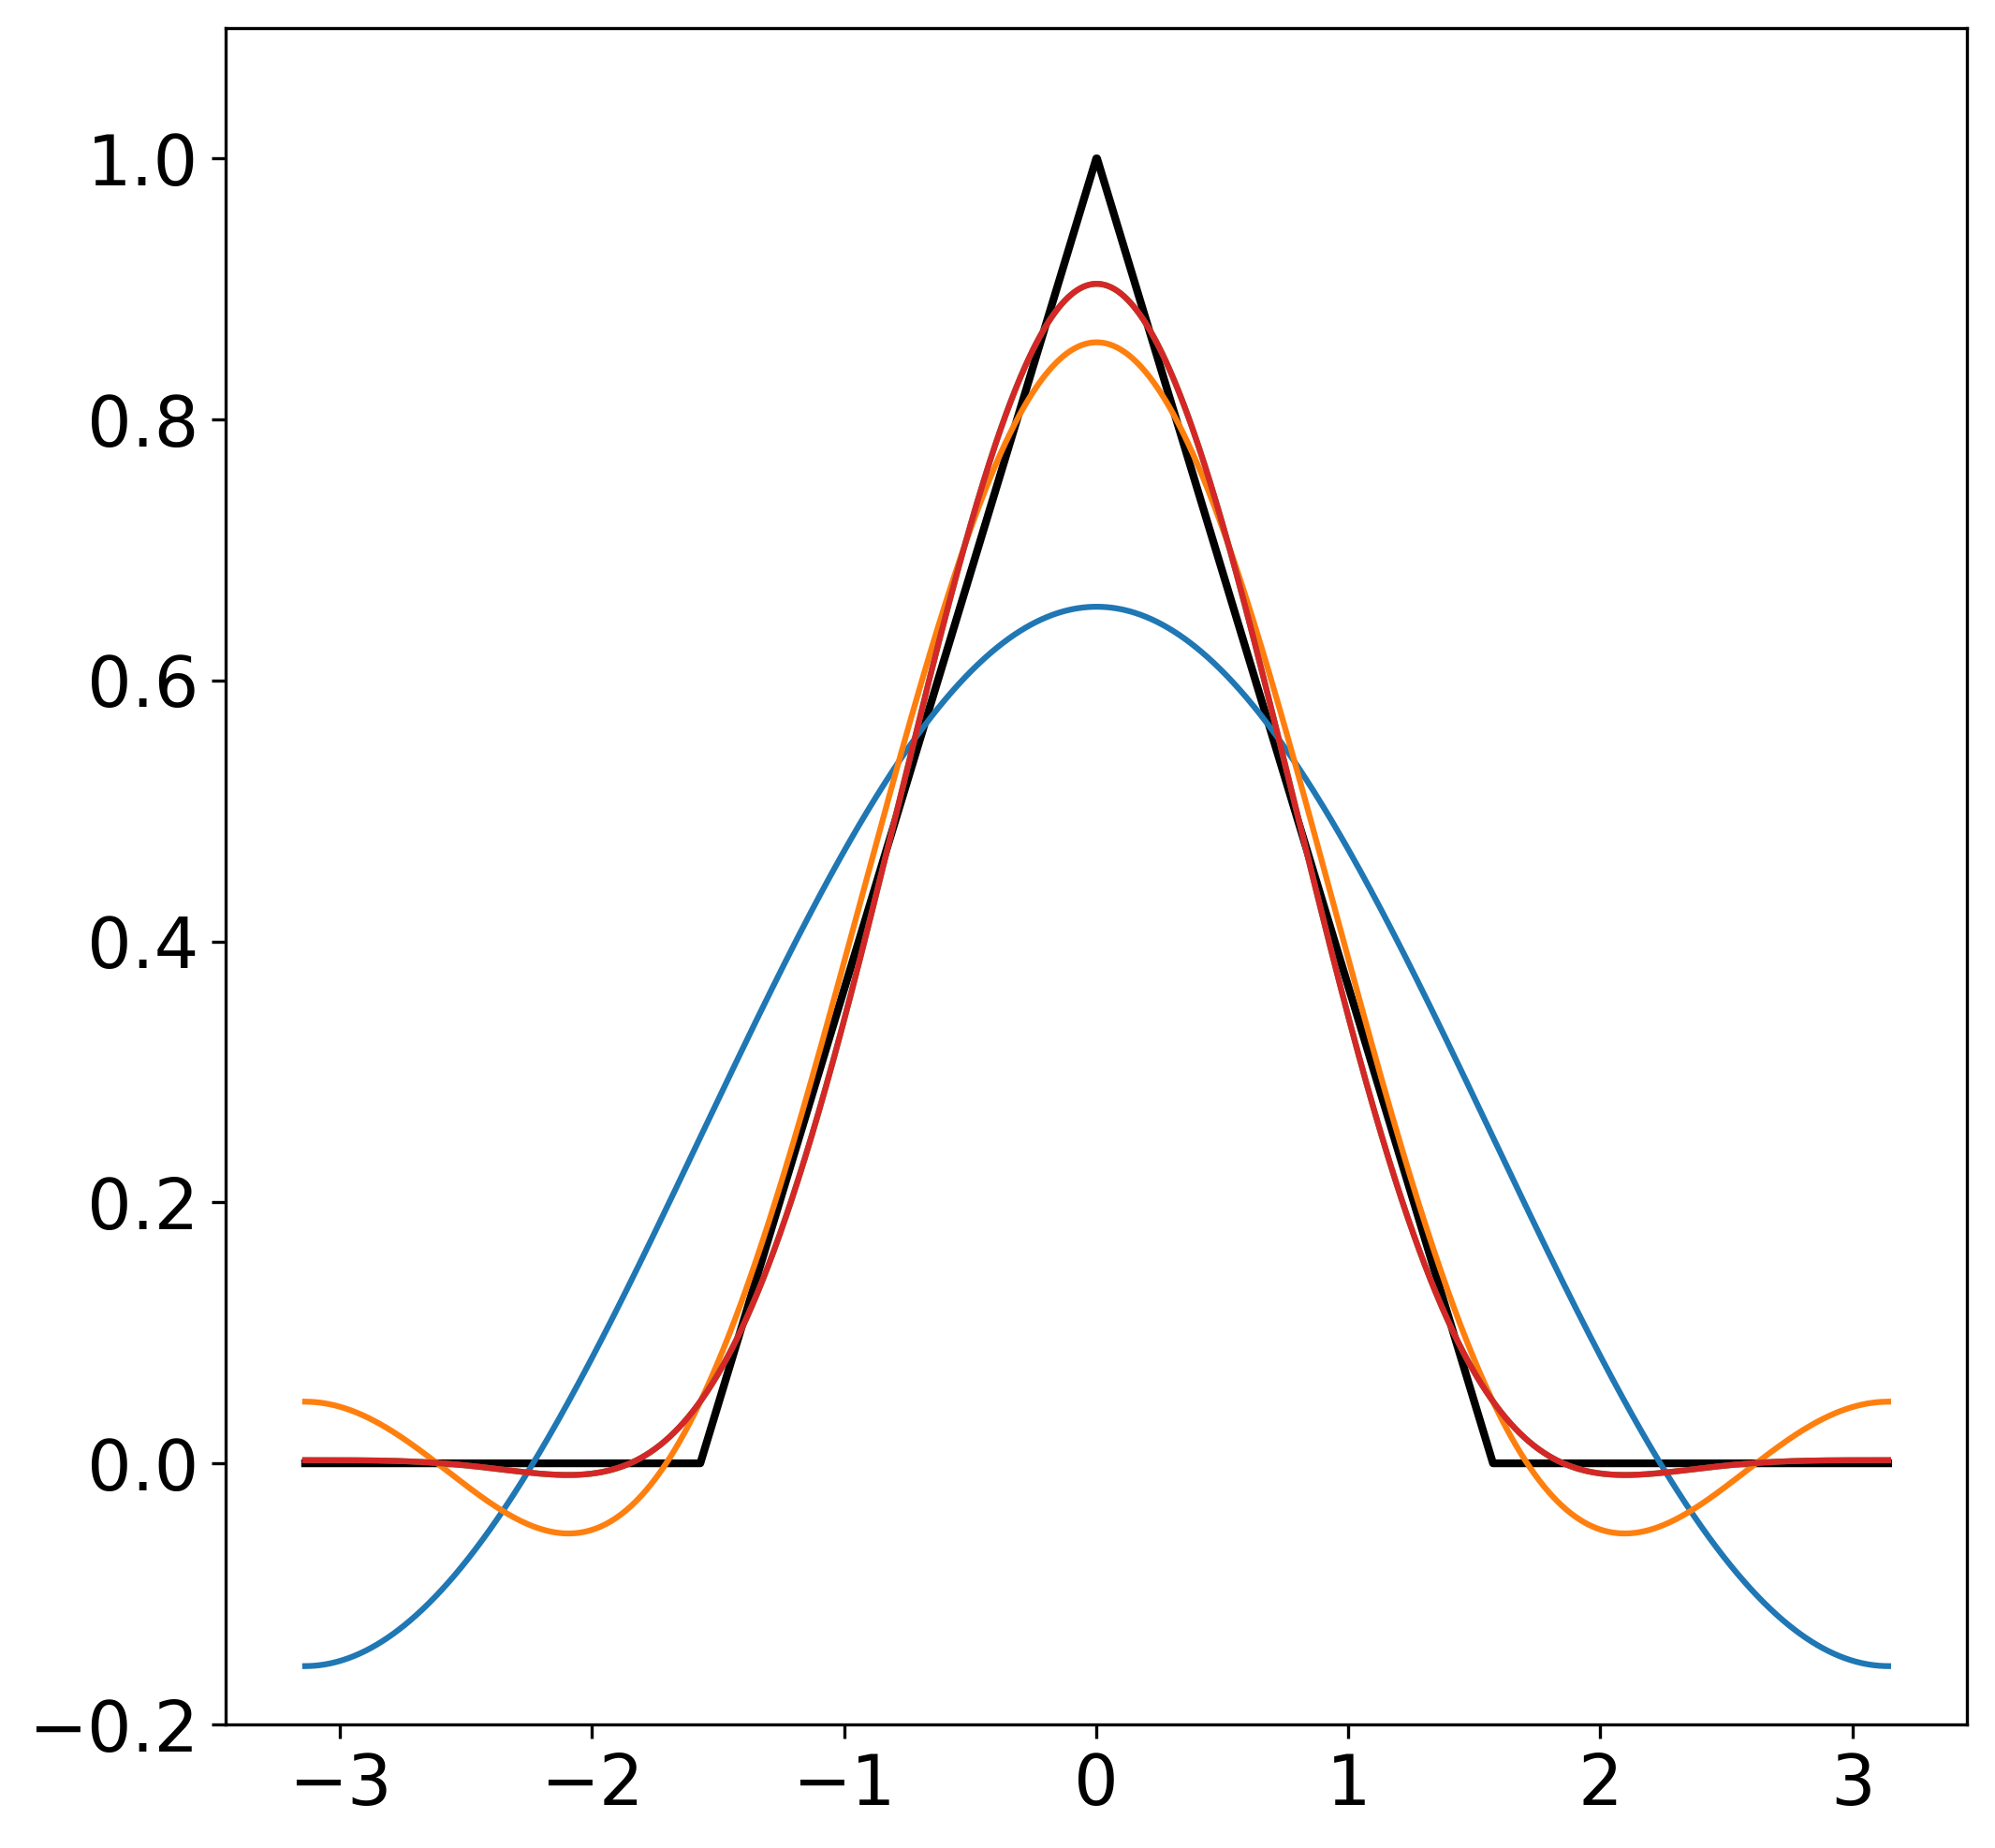
\includegraphics[width=.5\linewidth]{programs/fourier1/out_4.png}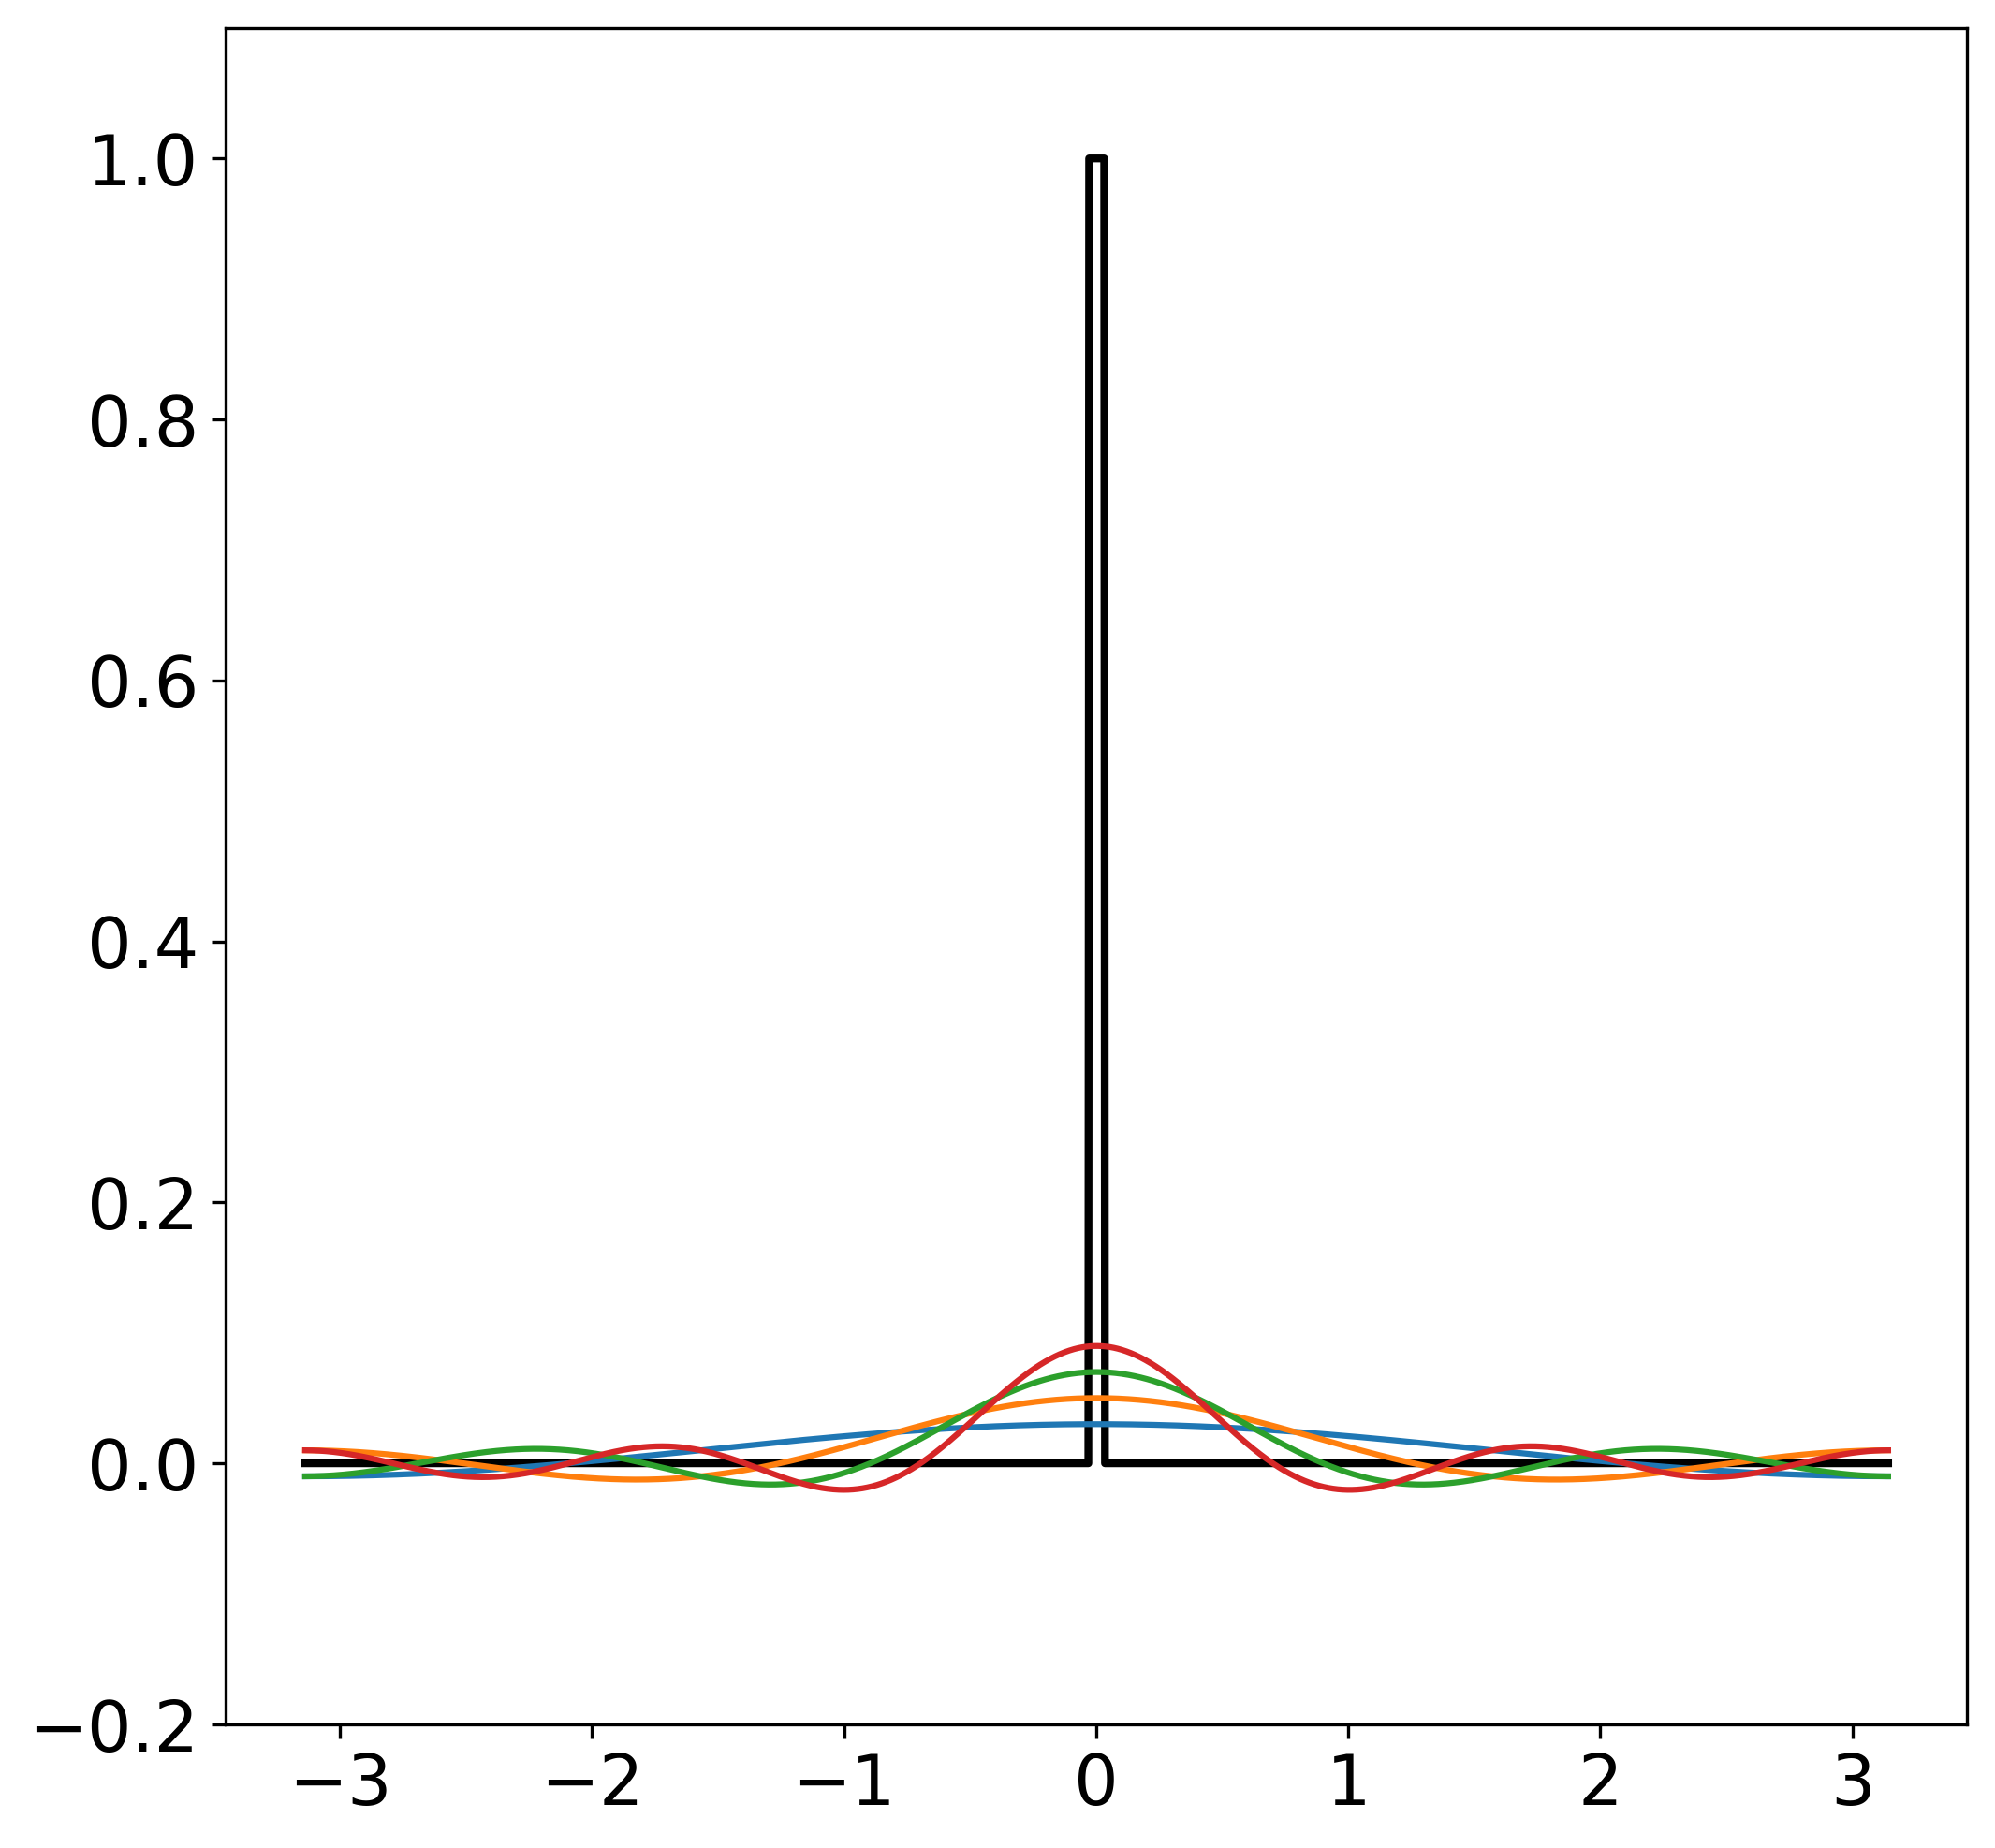
\includegraphics[width=.5\linewidth]{programs/fourier2/out_4.png}}
    \only<6|handout:0>{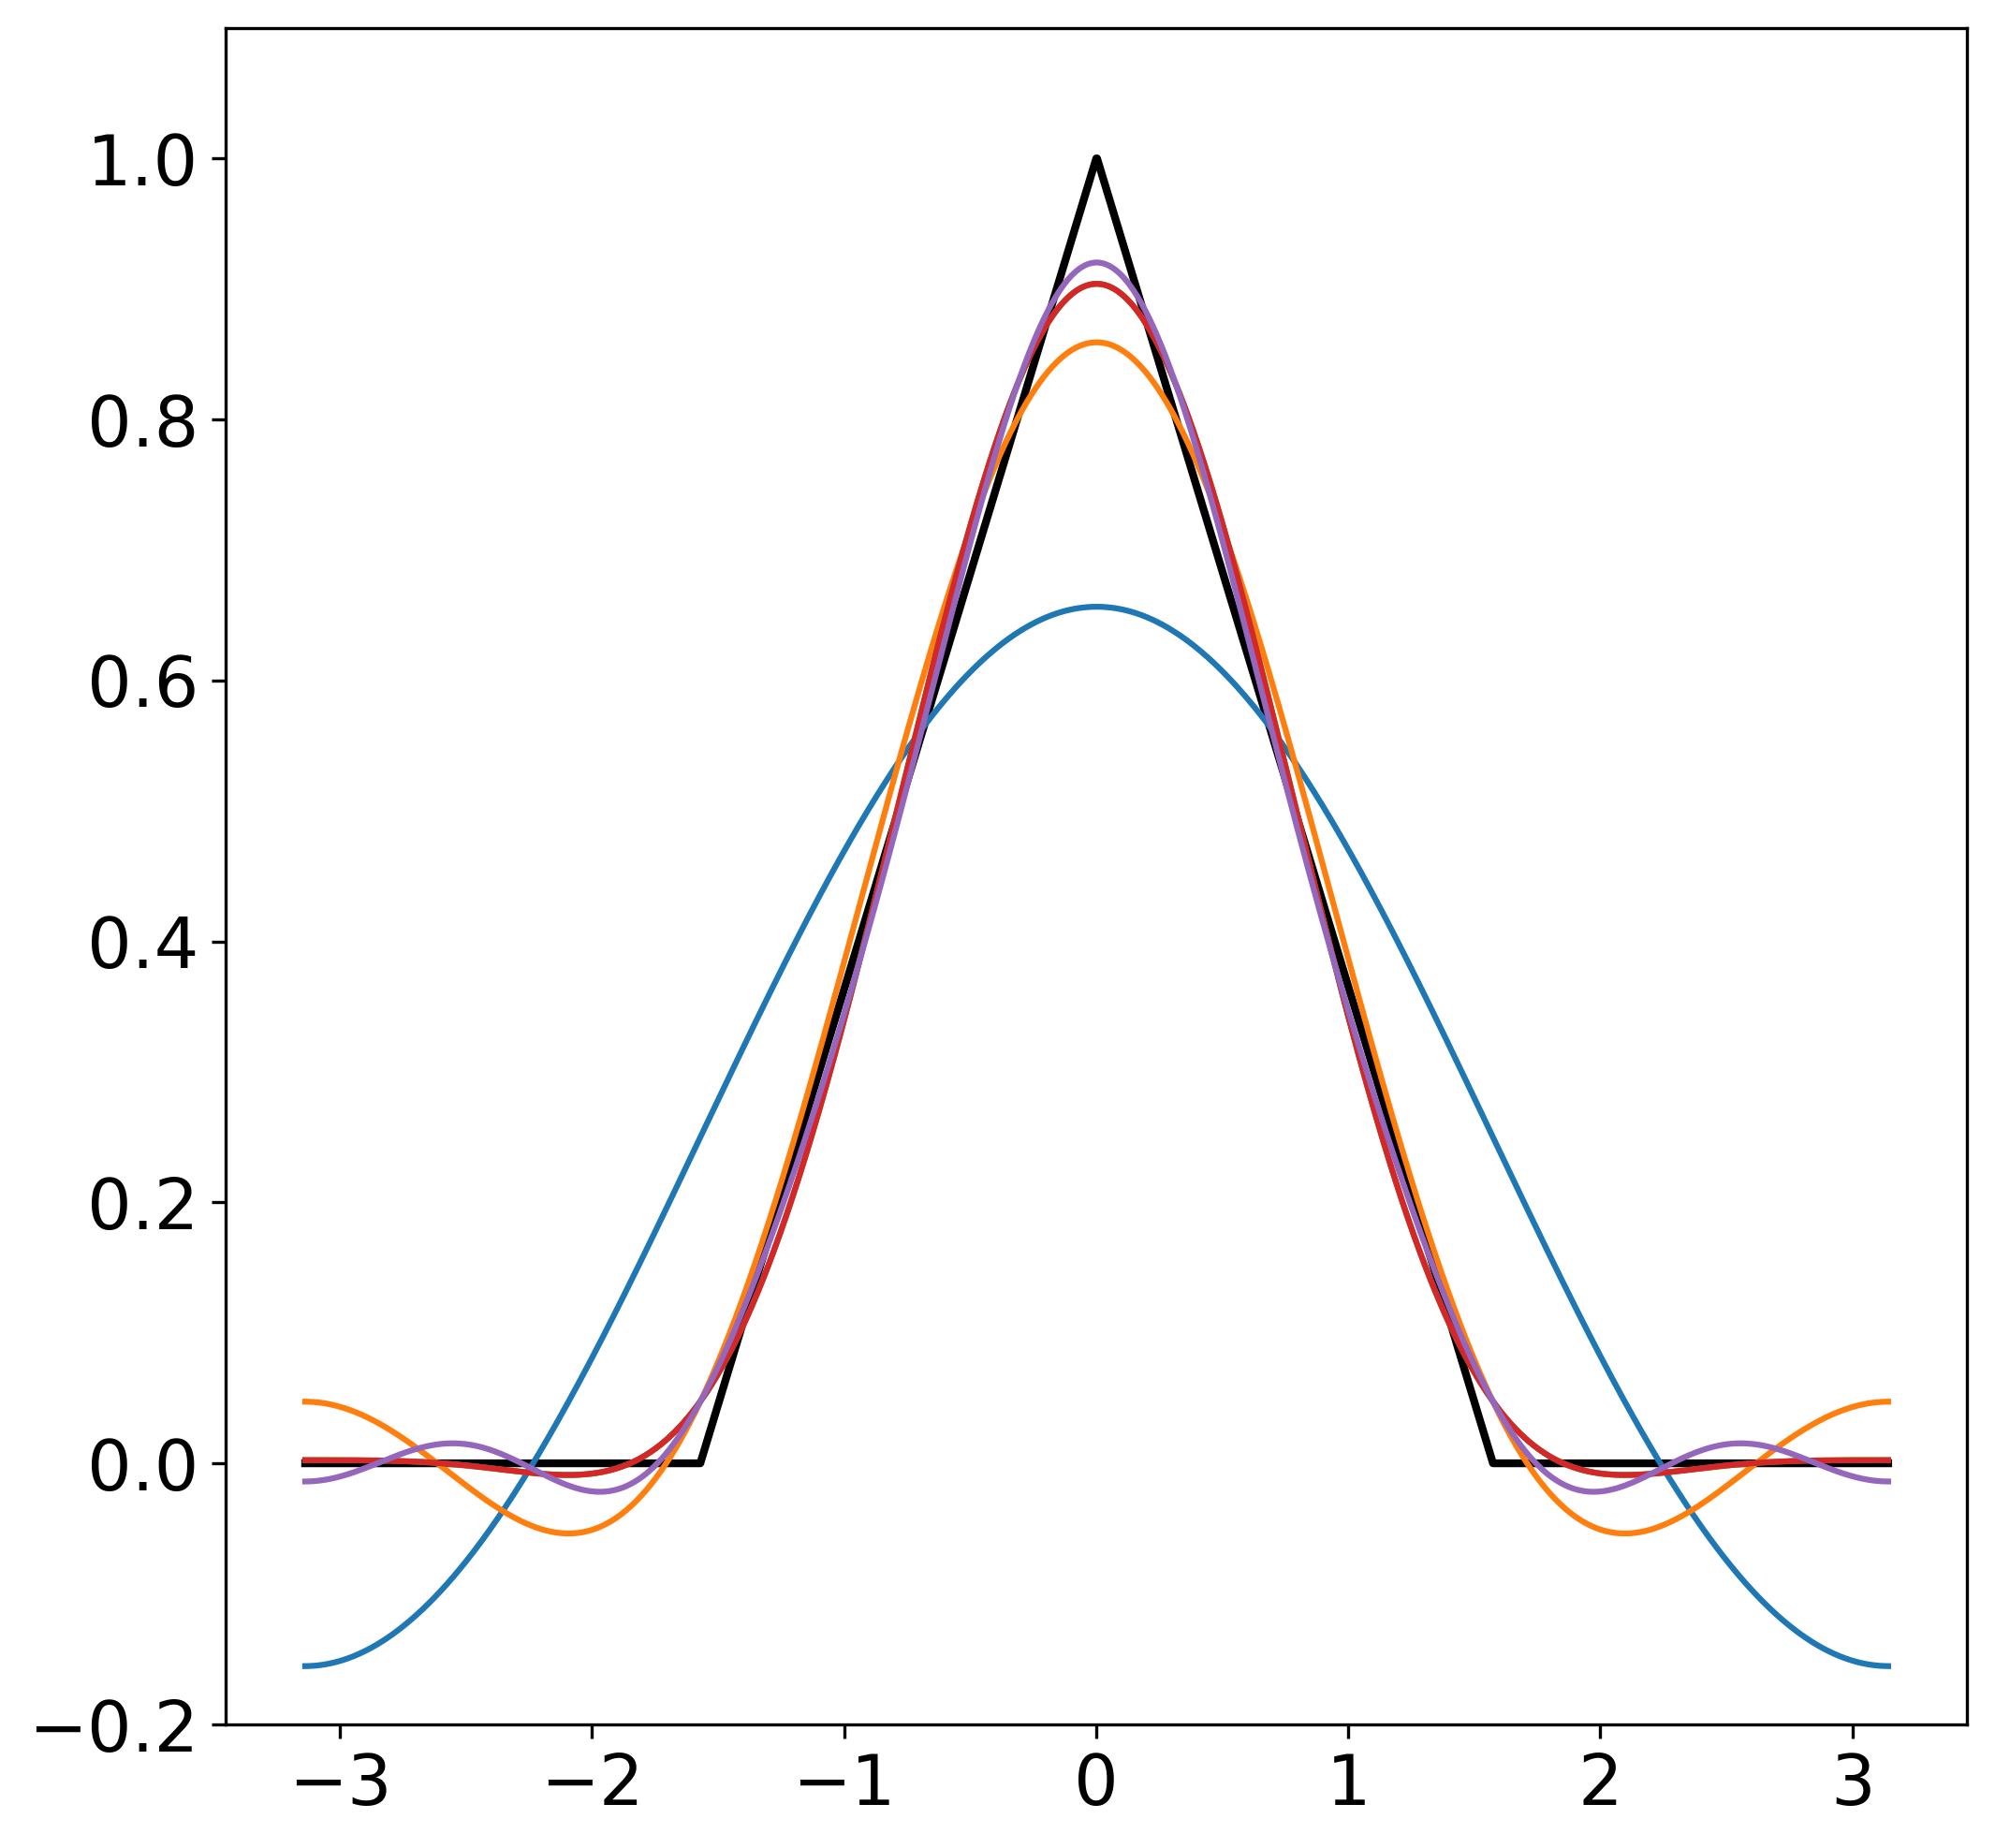
\includegraphics[width=.5\linewidth]{programs/fourier1/out_5.png}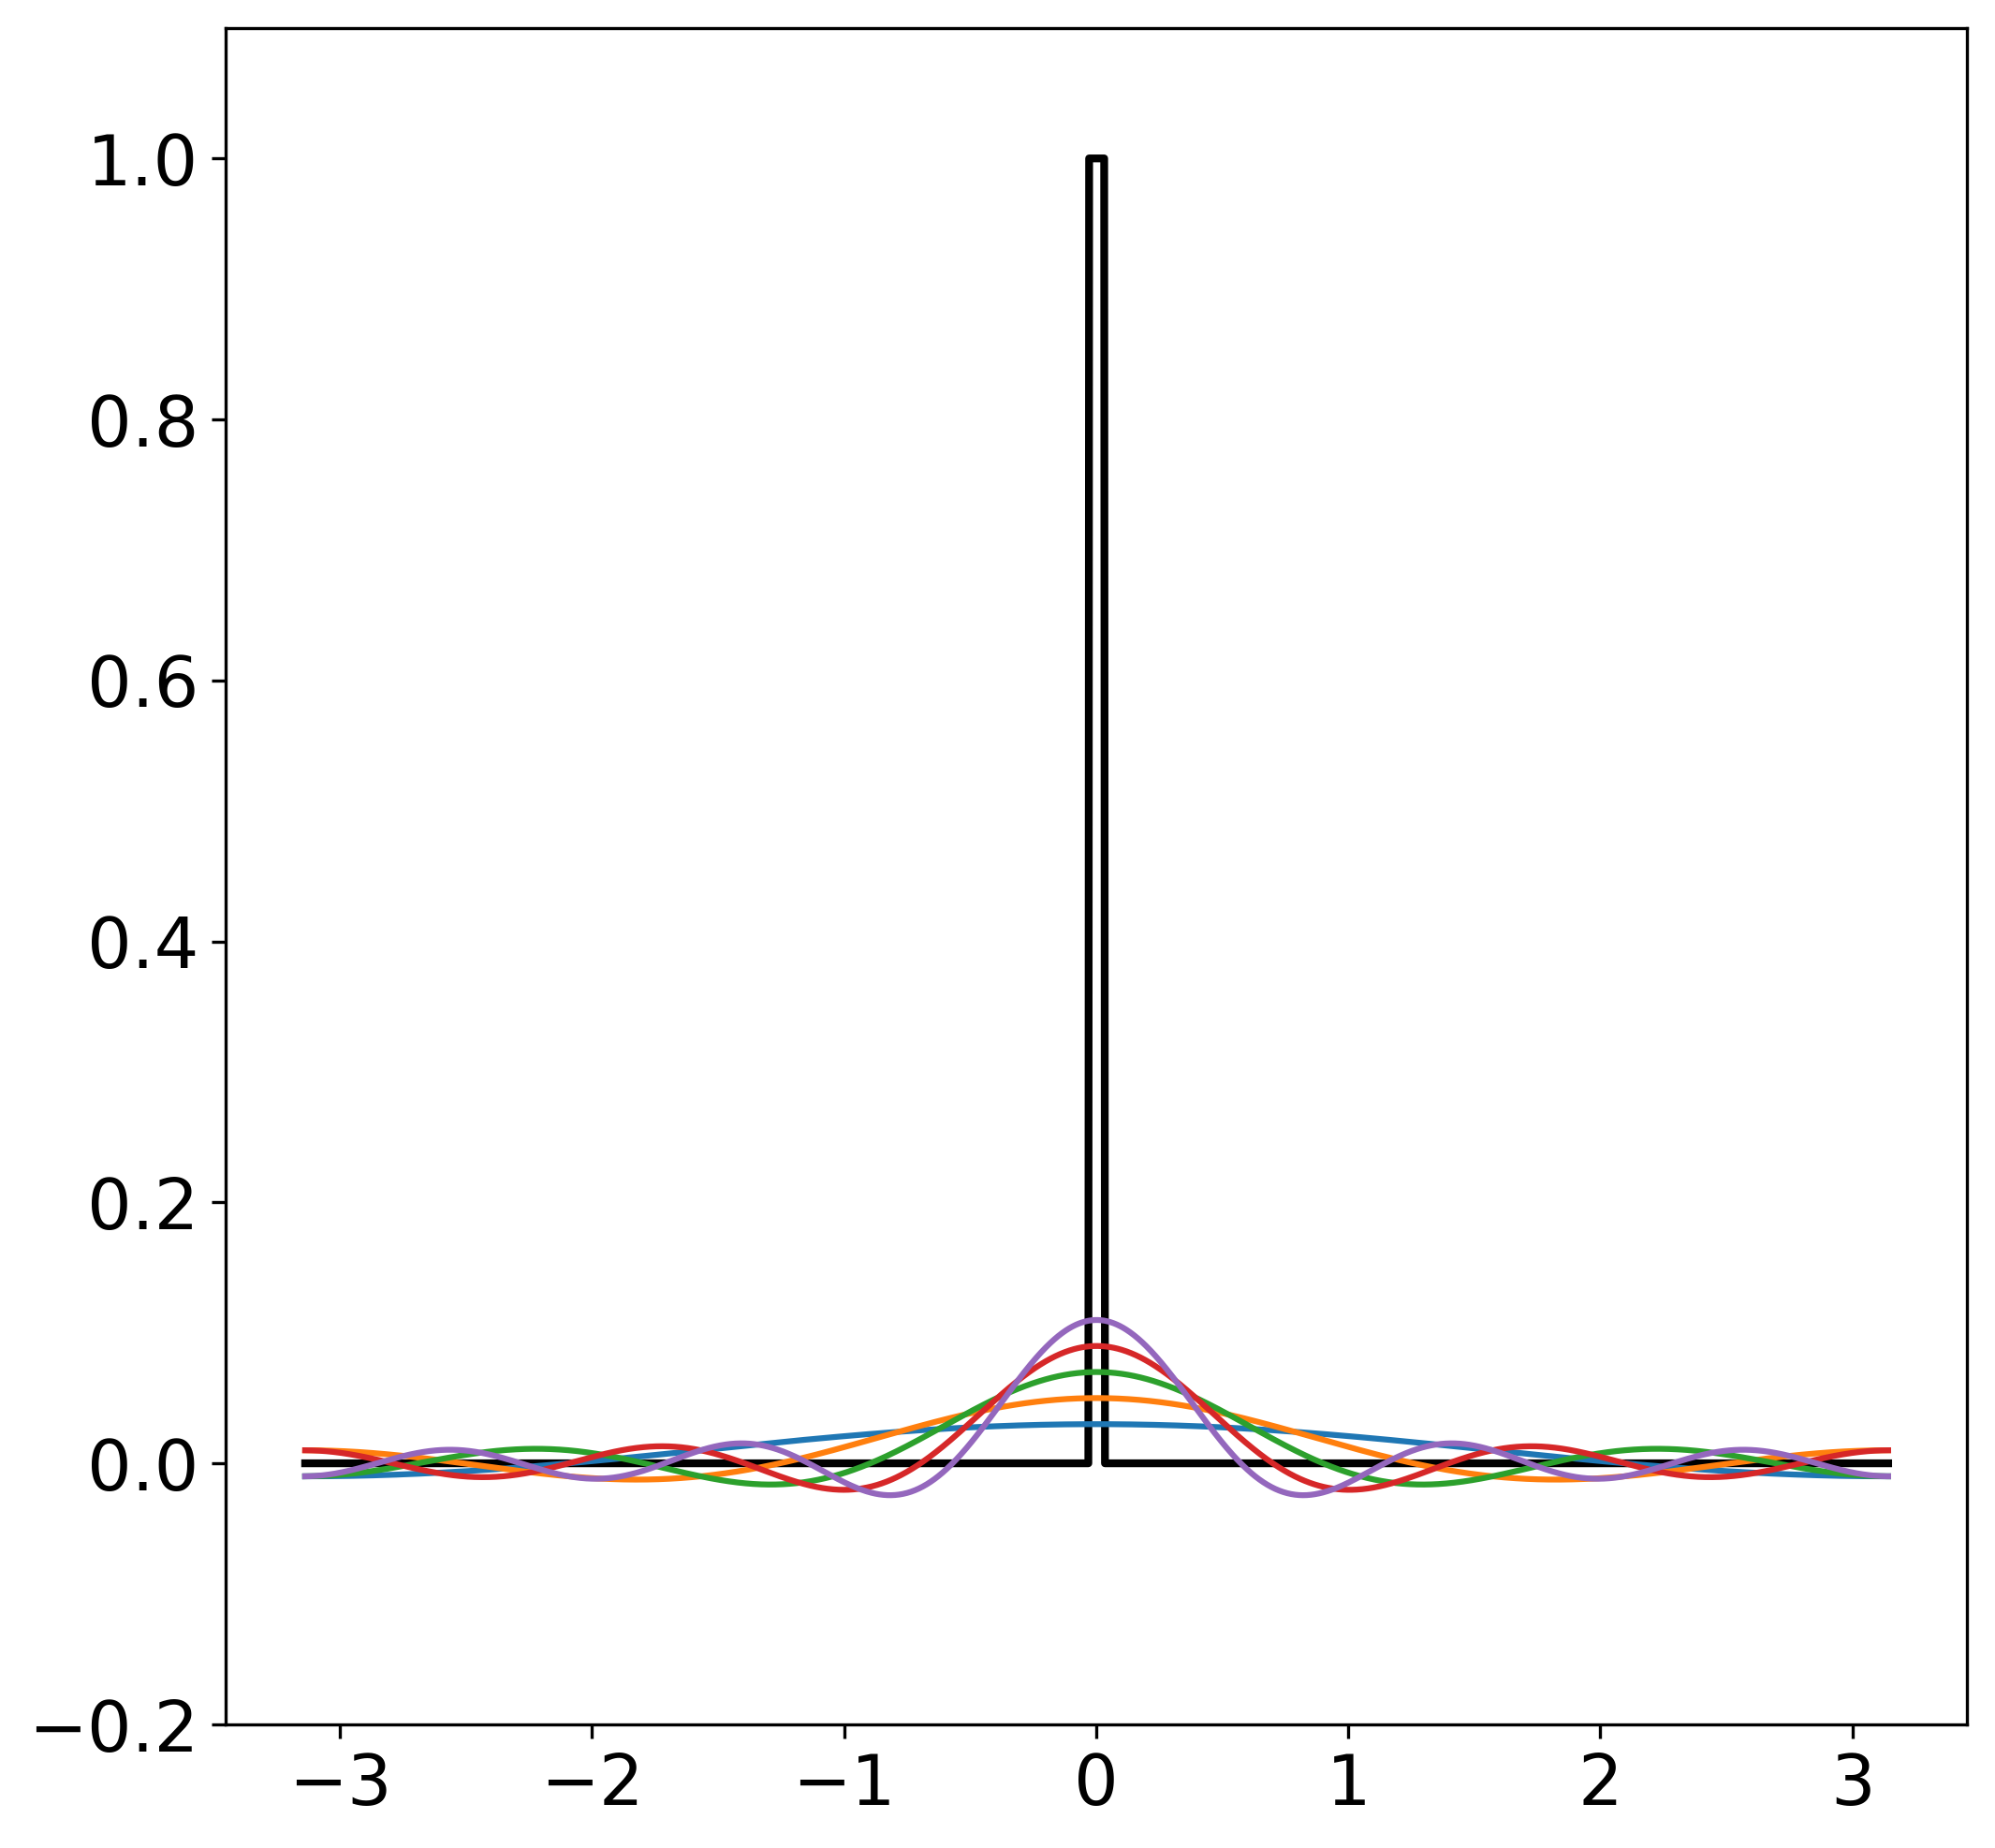
\includegraphics[width=.5\linewidth]{programs/fourier2/out_5.png}}
    \only<7|handout:0>{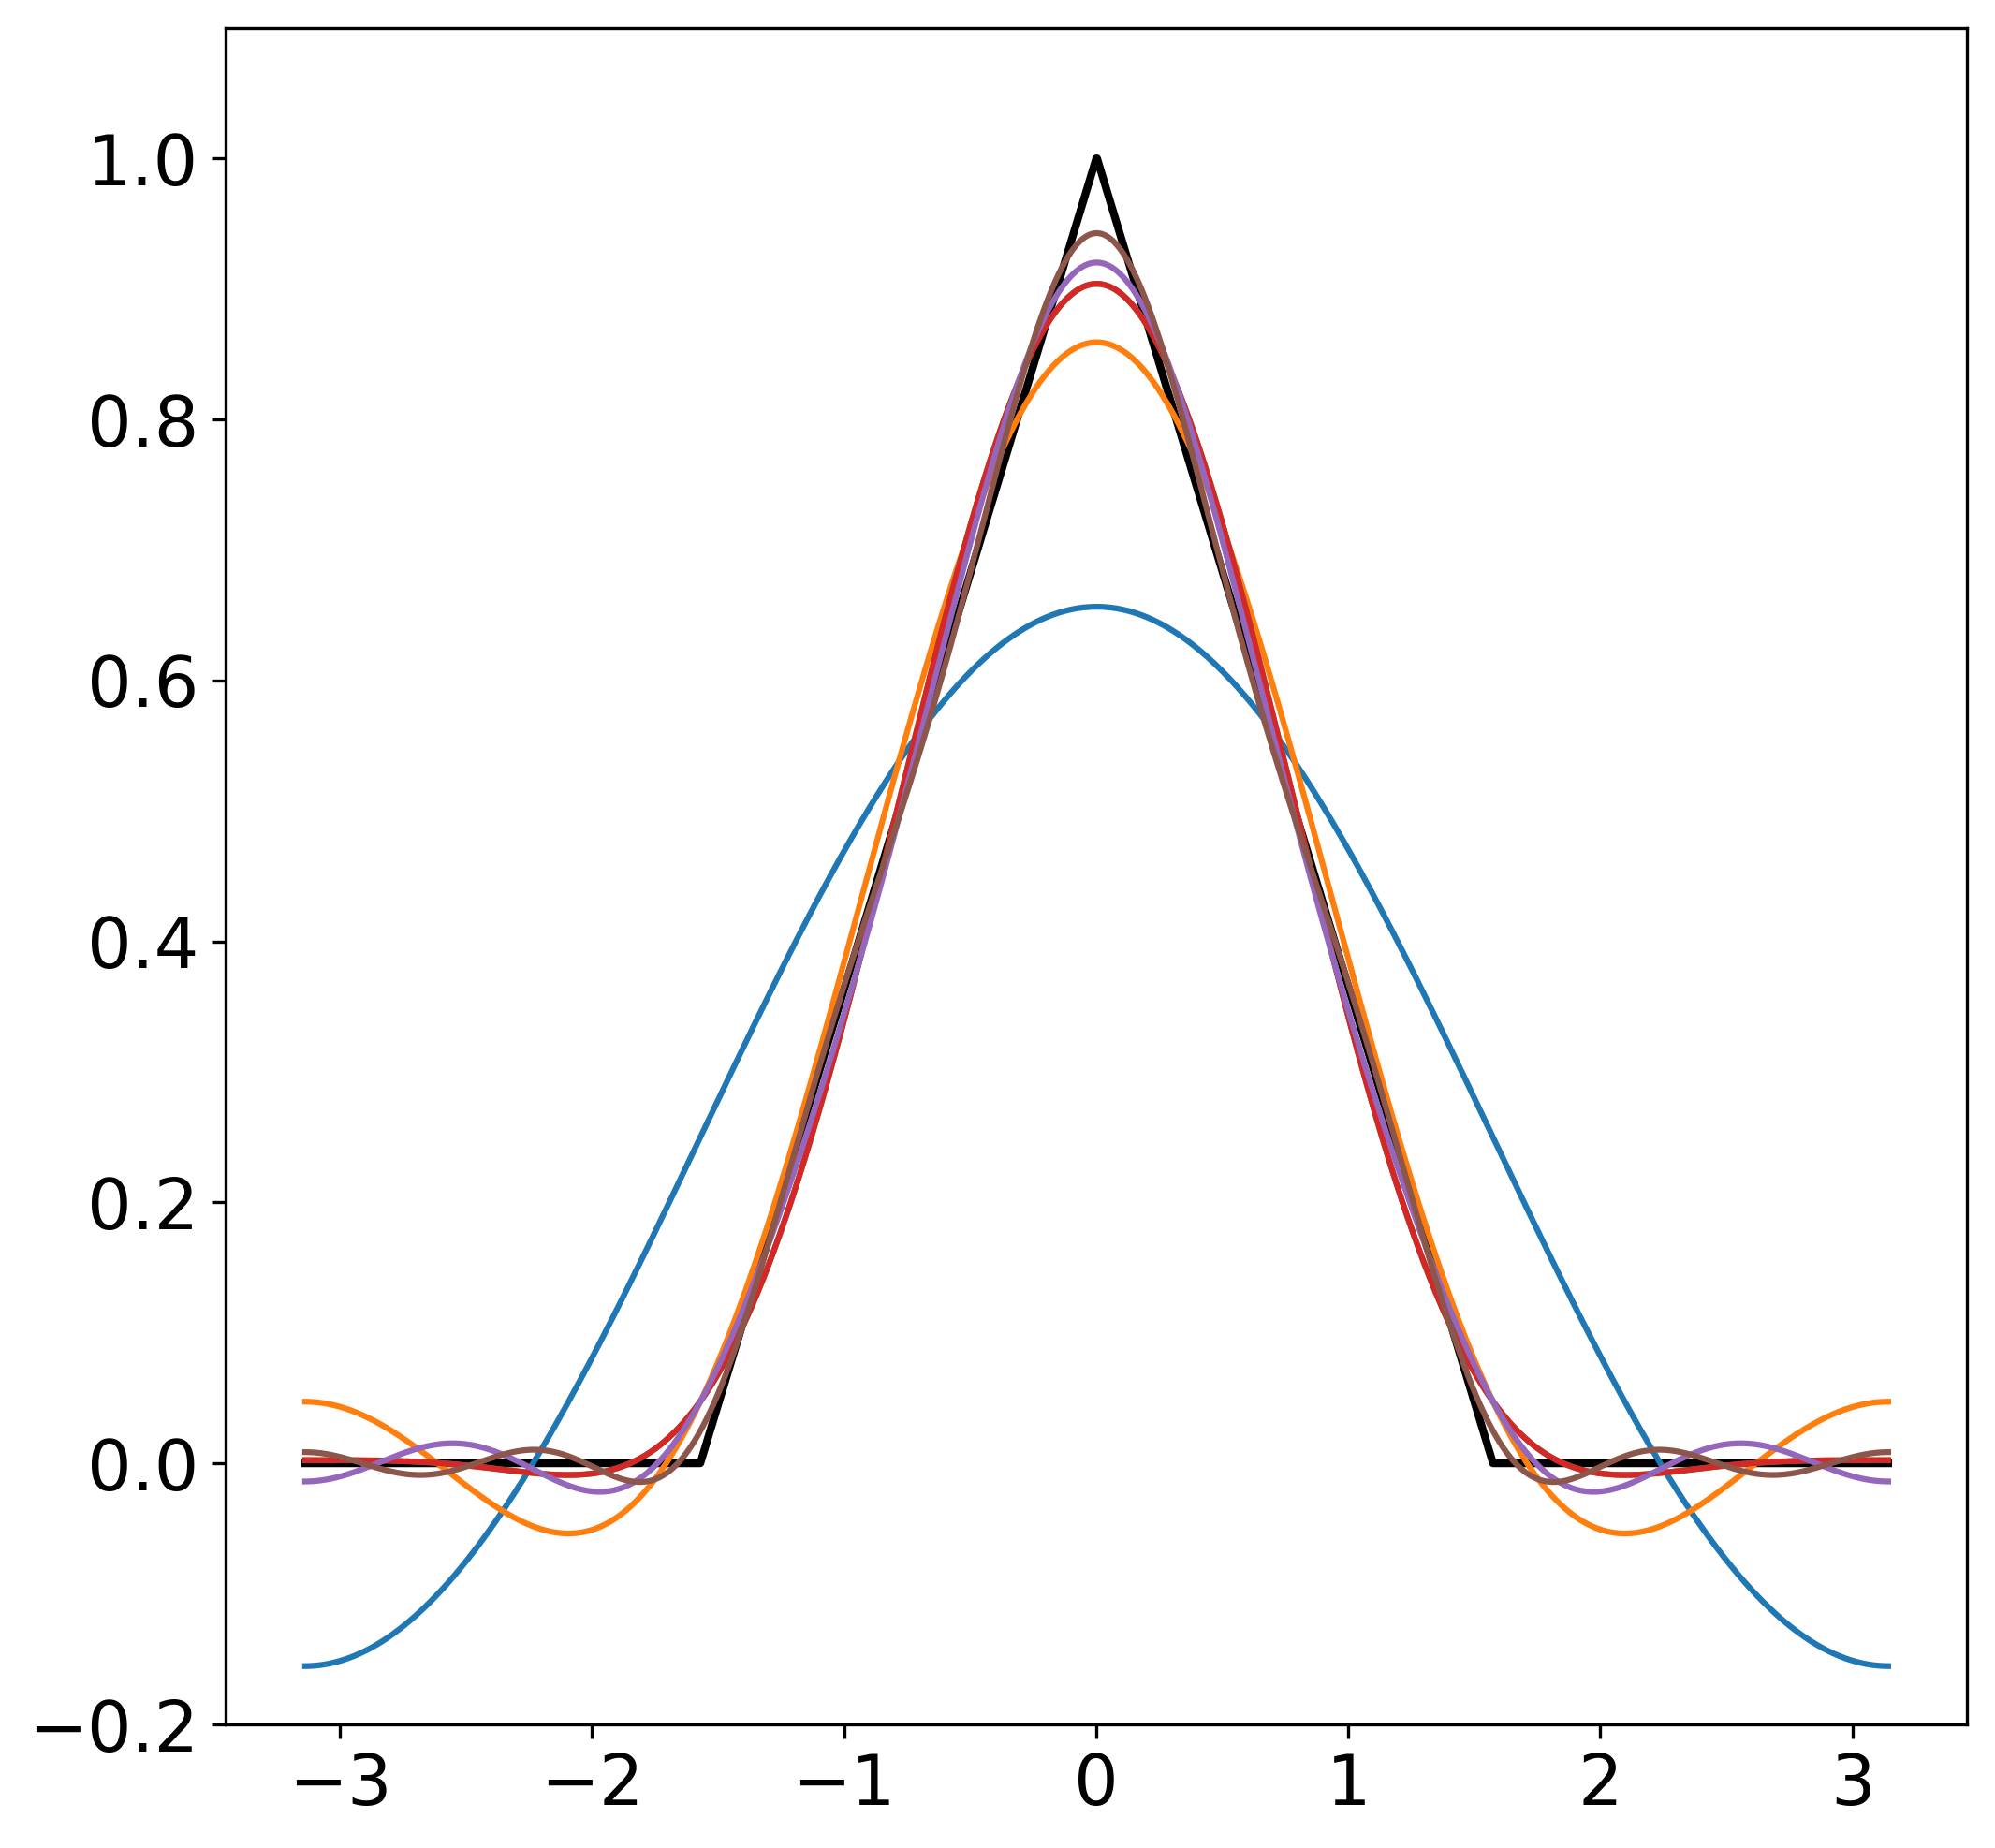
\includegraphics[width=.5\linewidth]{programs/fourier1/out_6.png}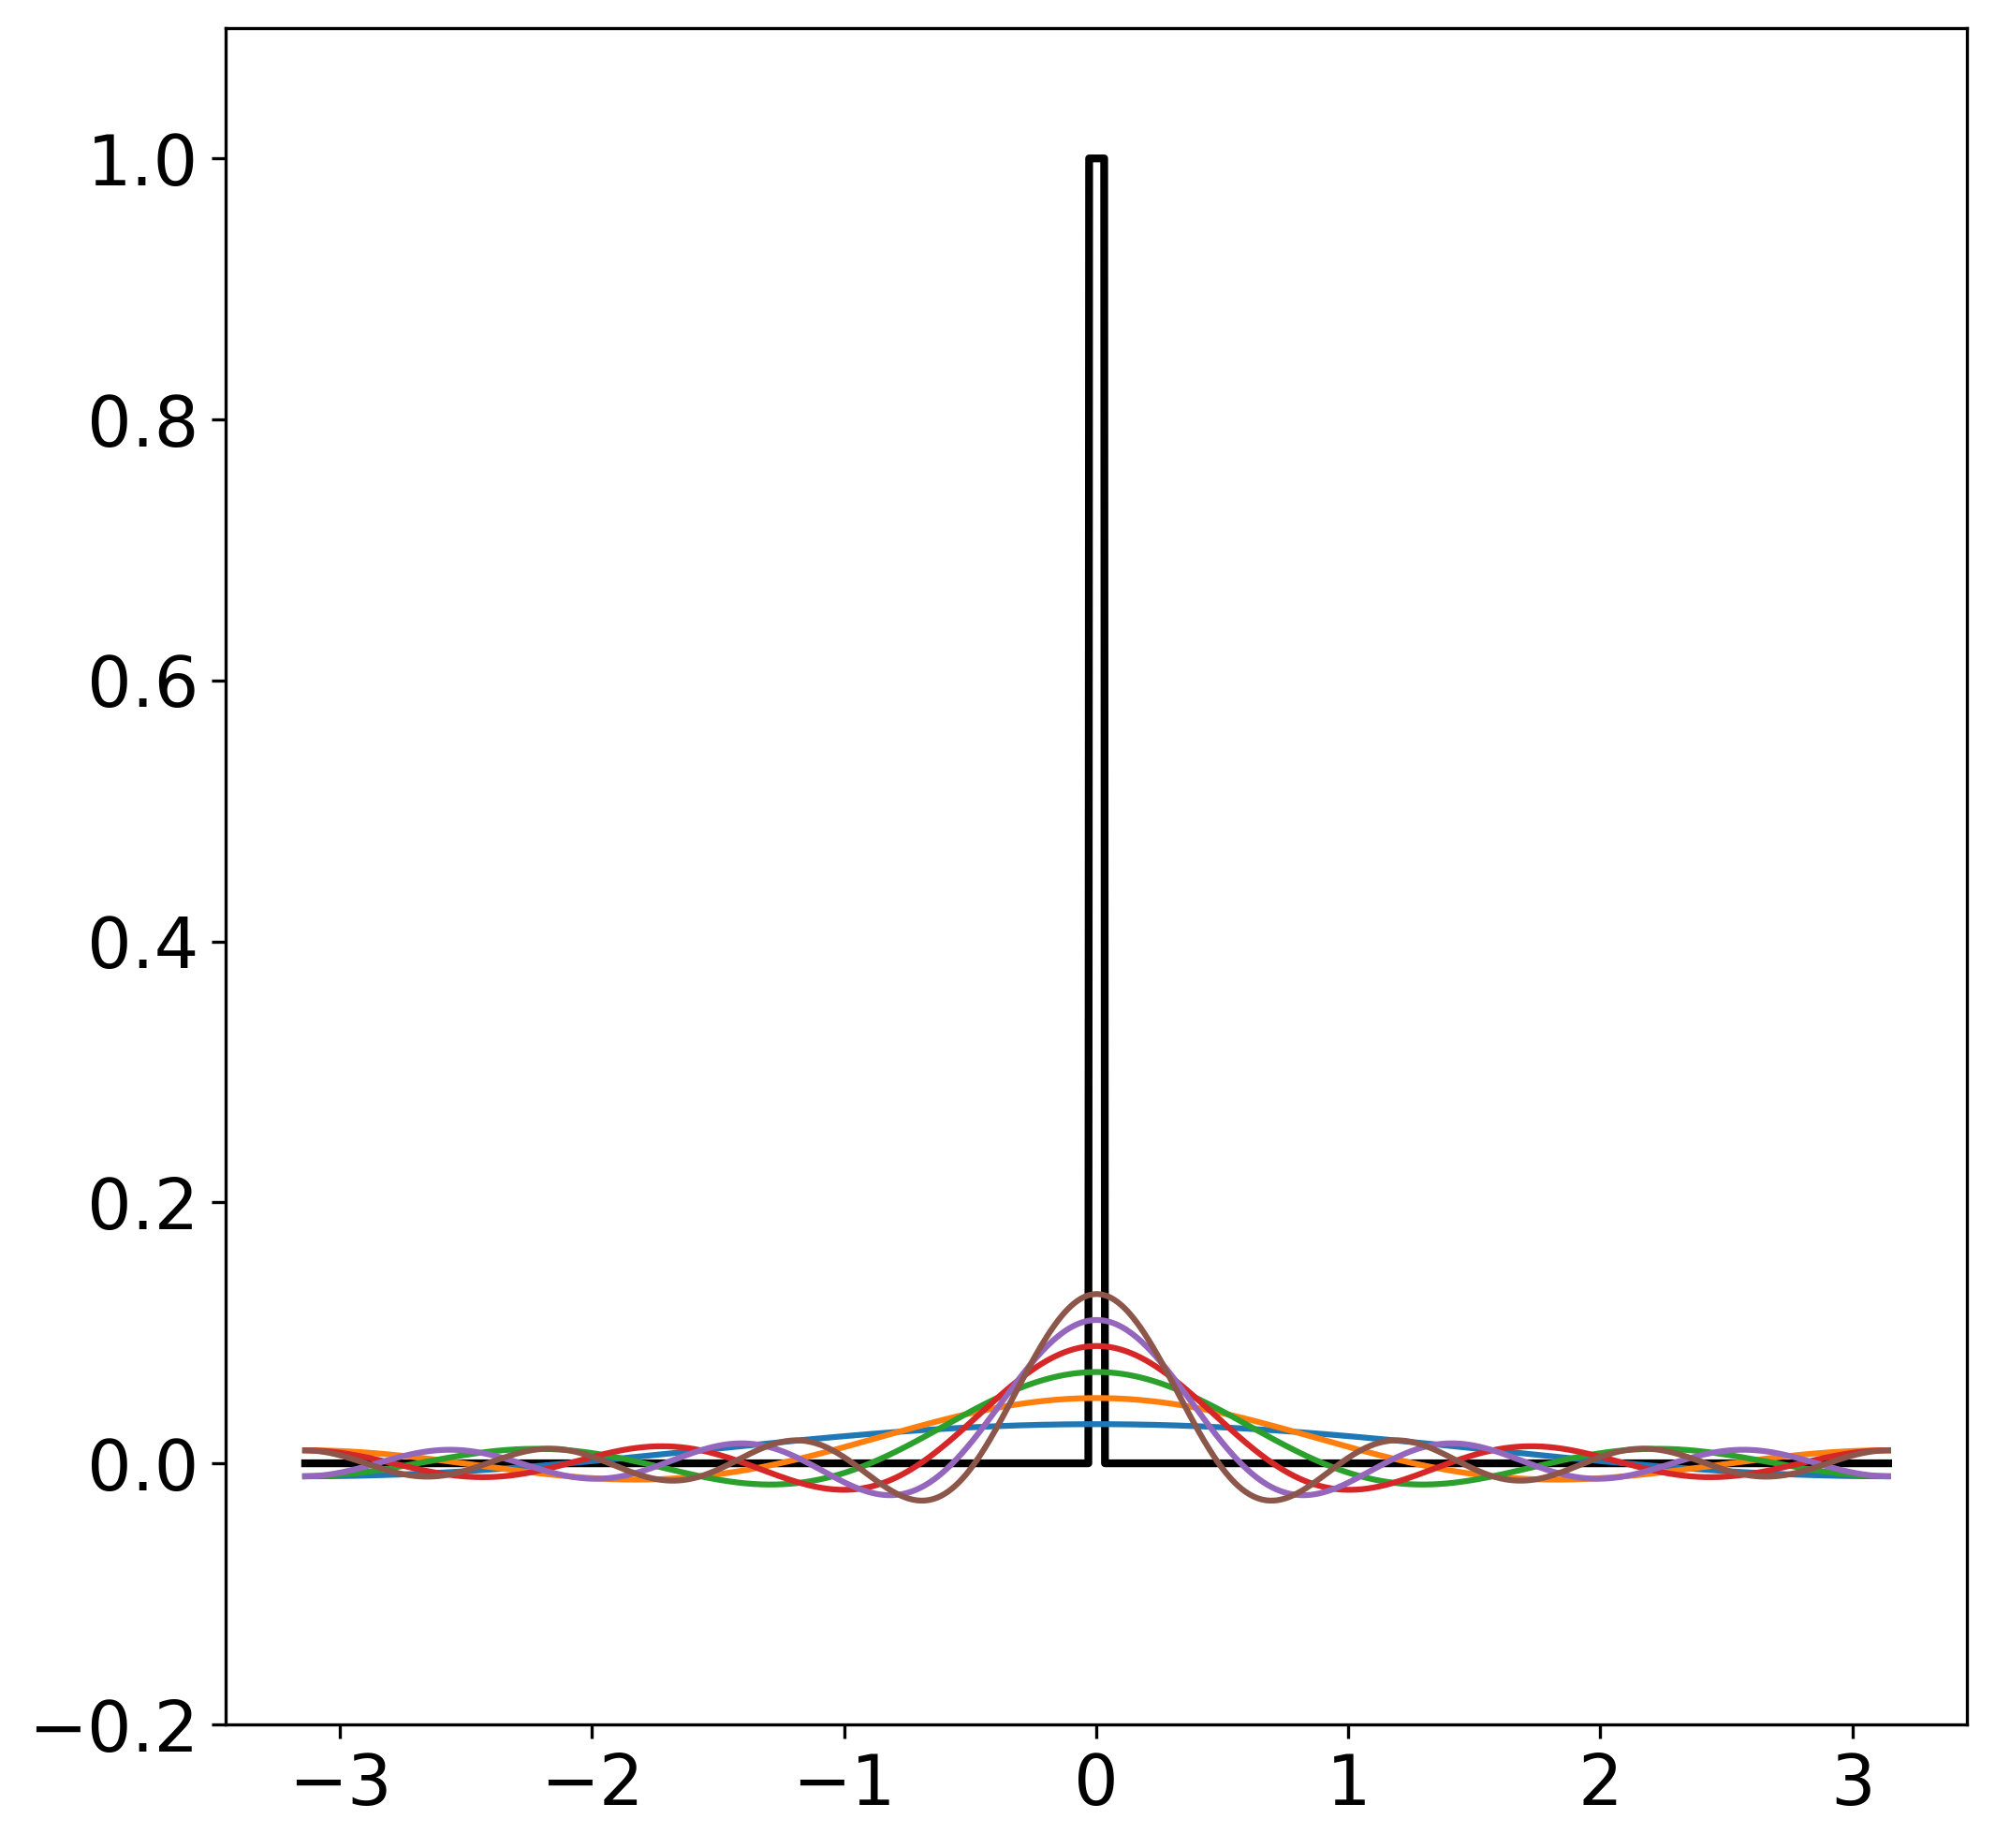
\includegraphics[width=.5\linewidth]{programs/fourier2/out_6.png}}
    \only<8|handout:0>{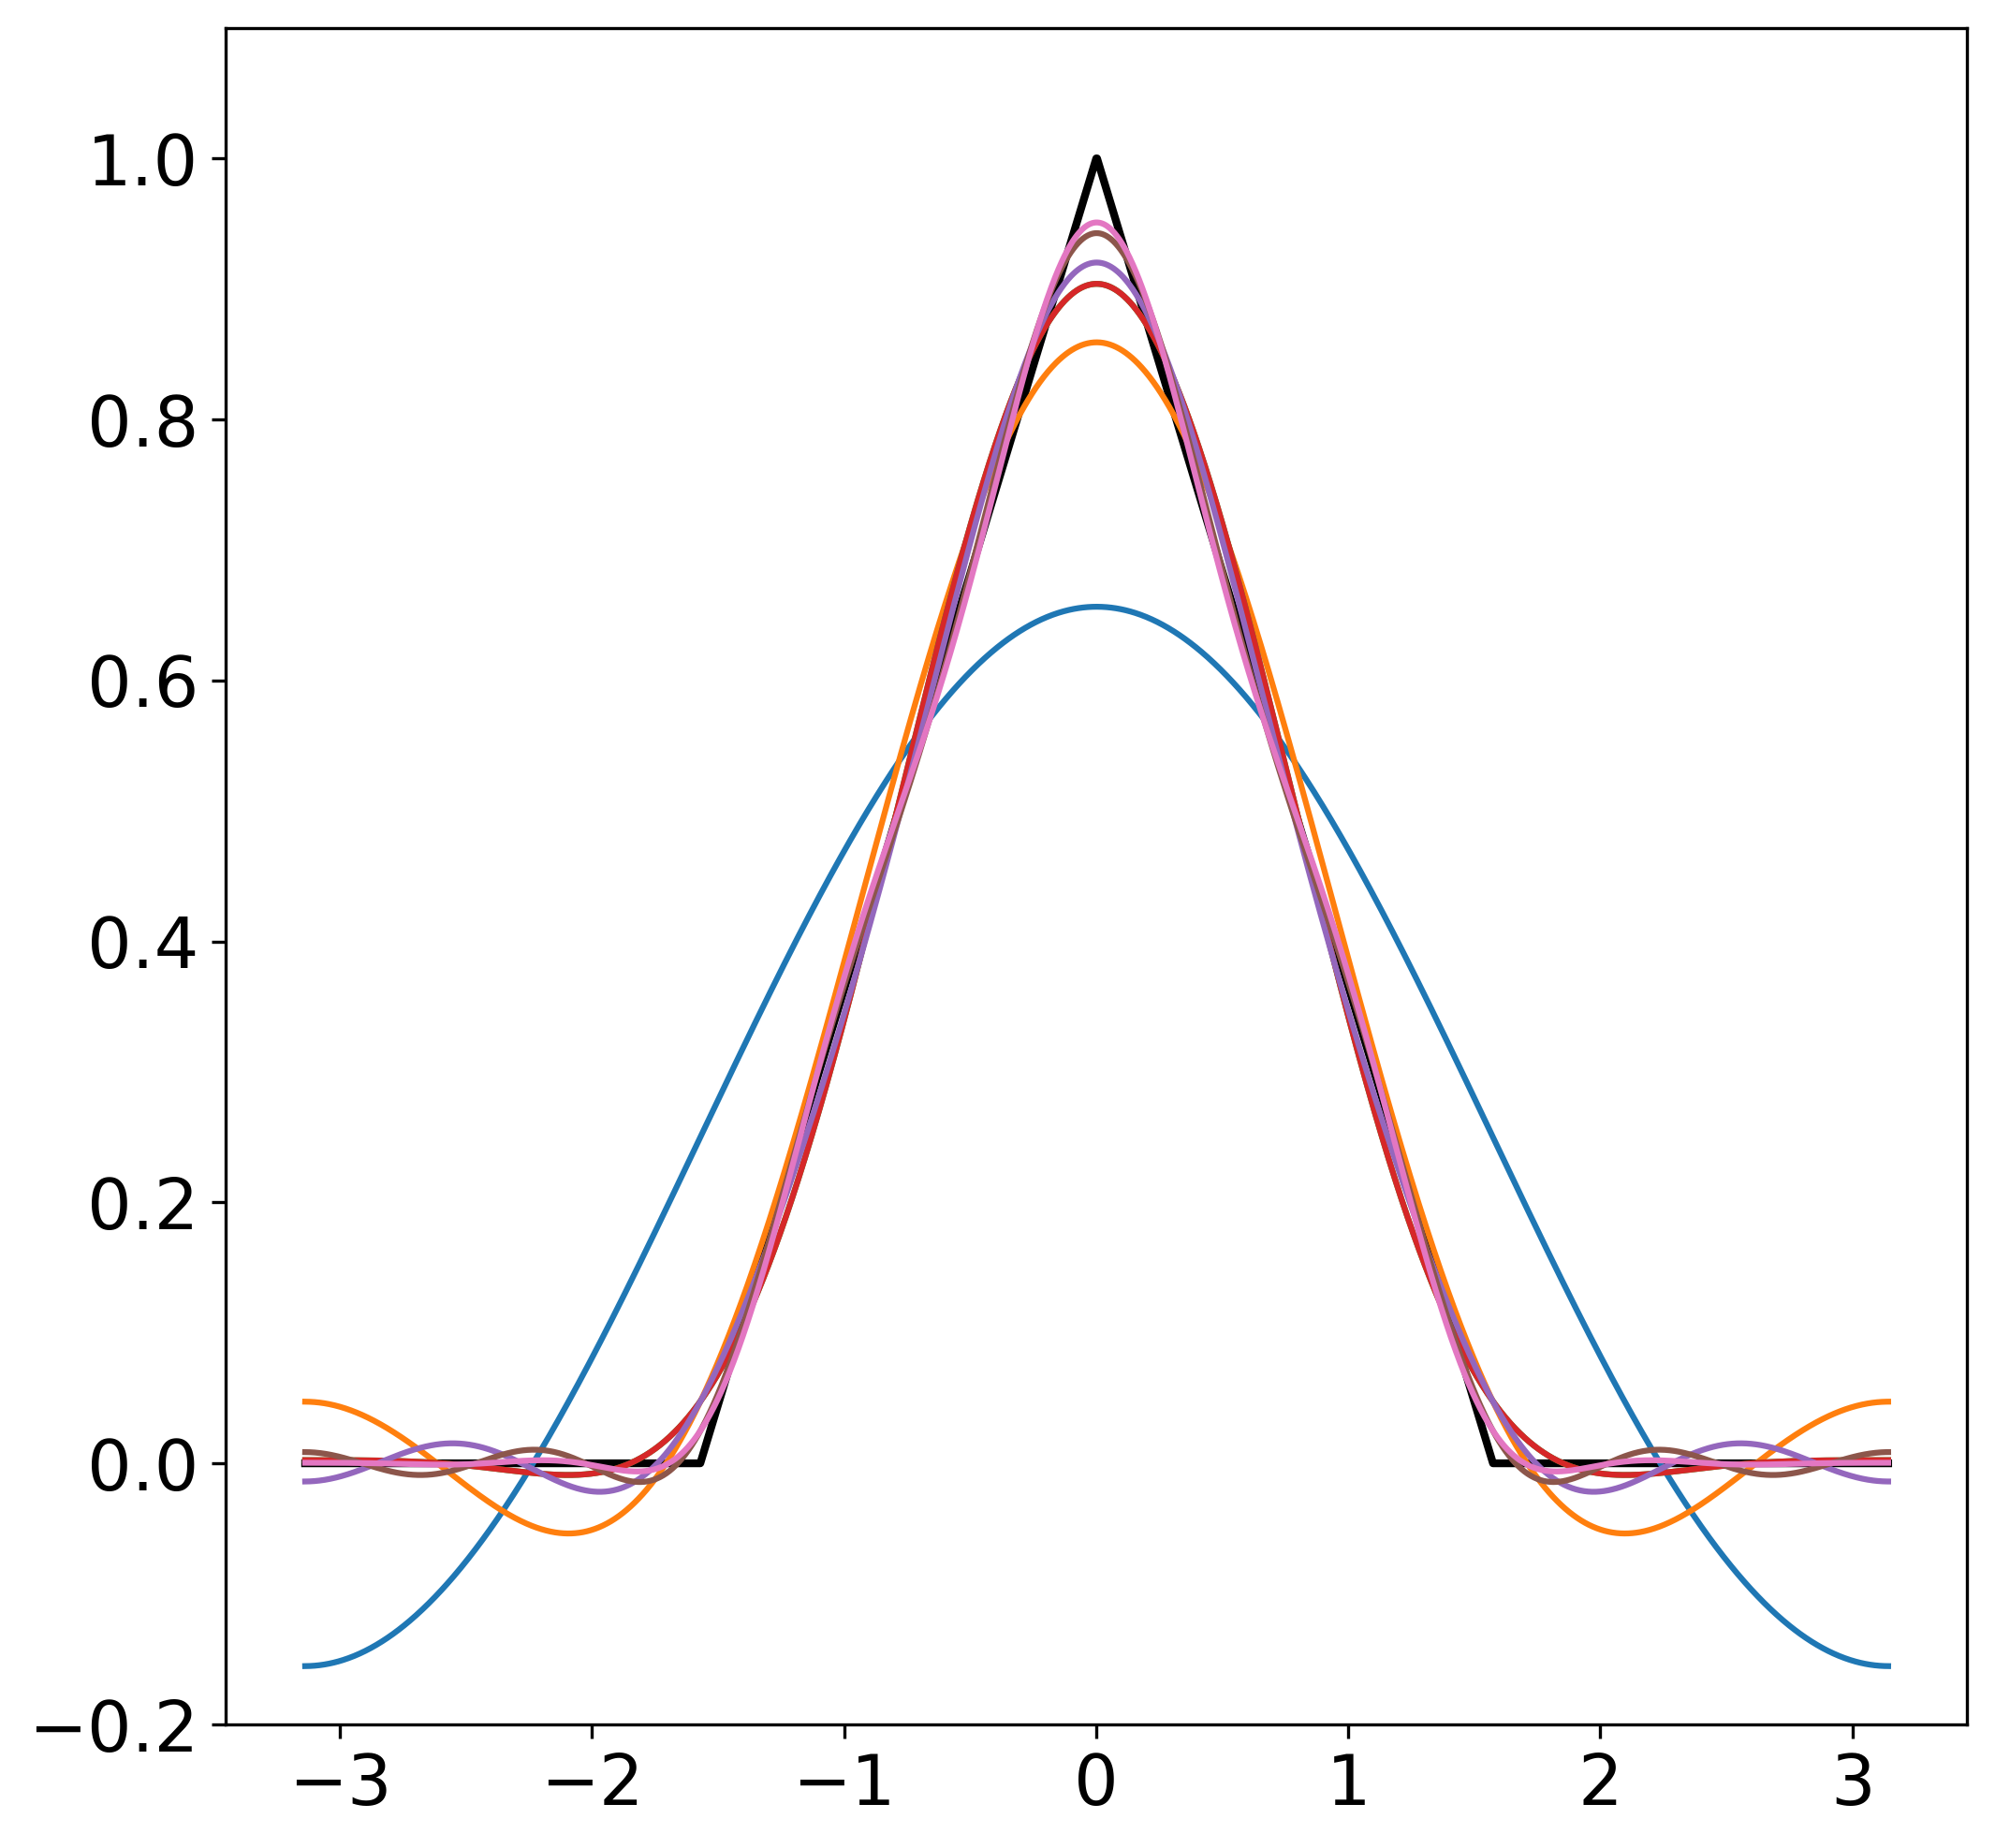
\includegraphics[width=.5\linewidth]{programs/fourier1/out_7.png}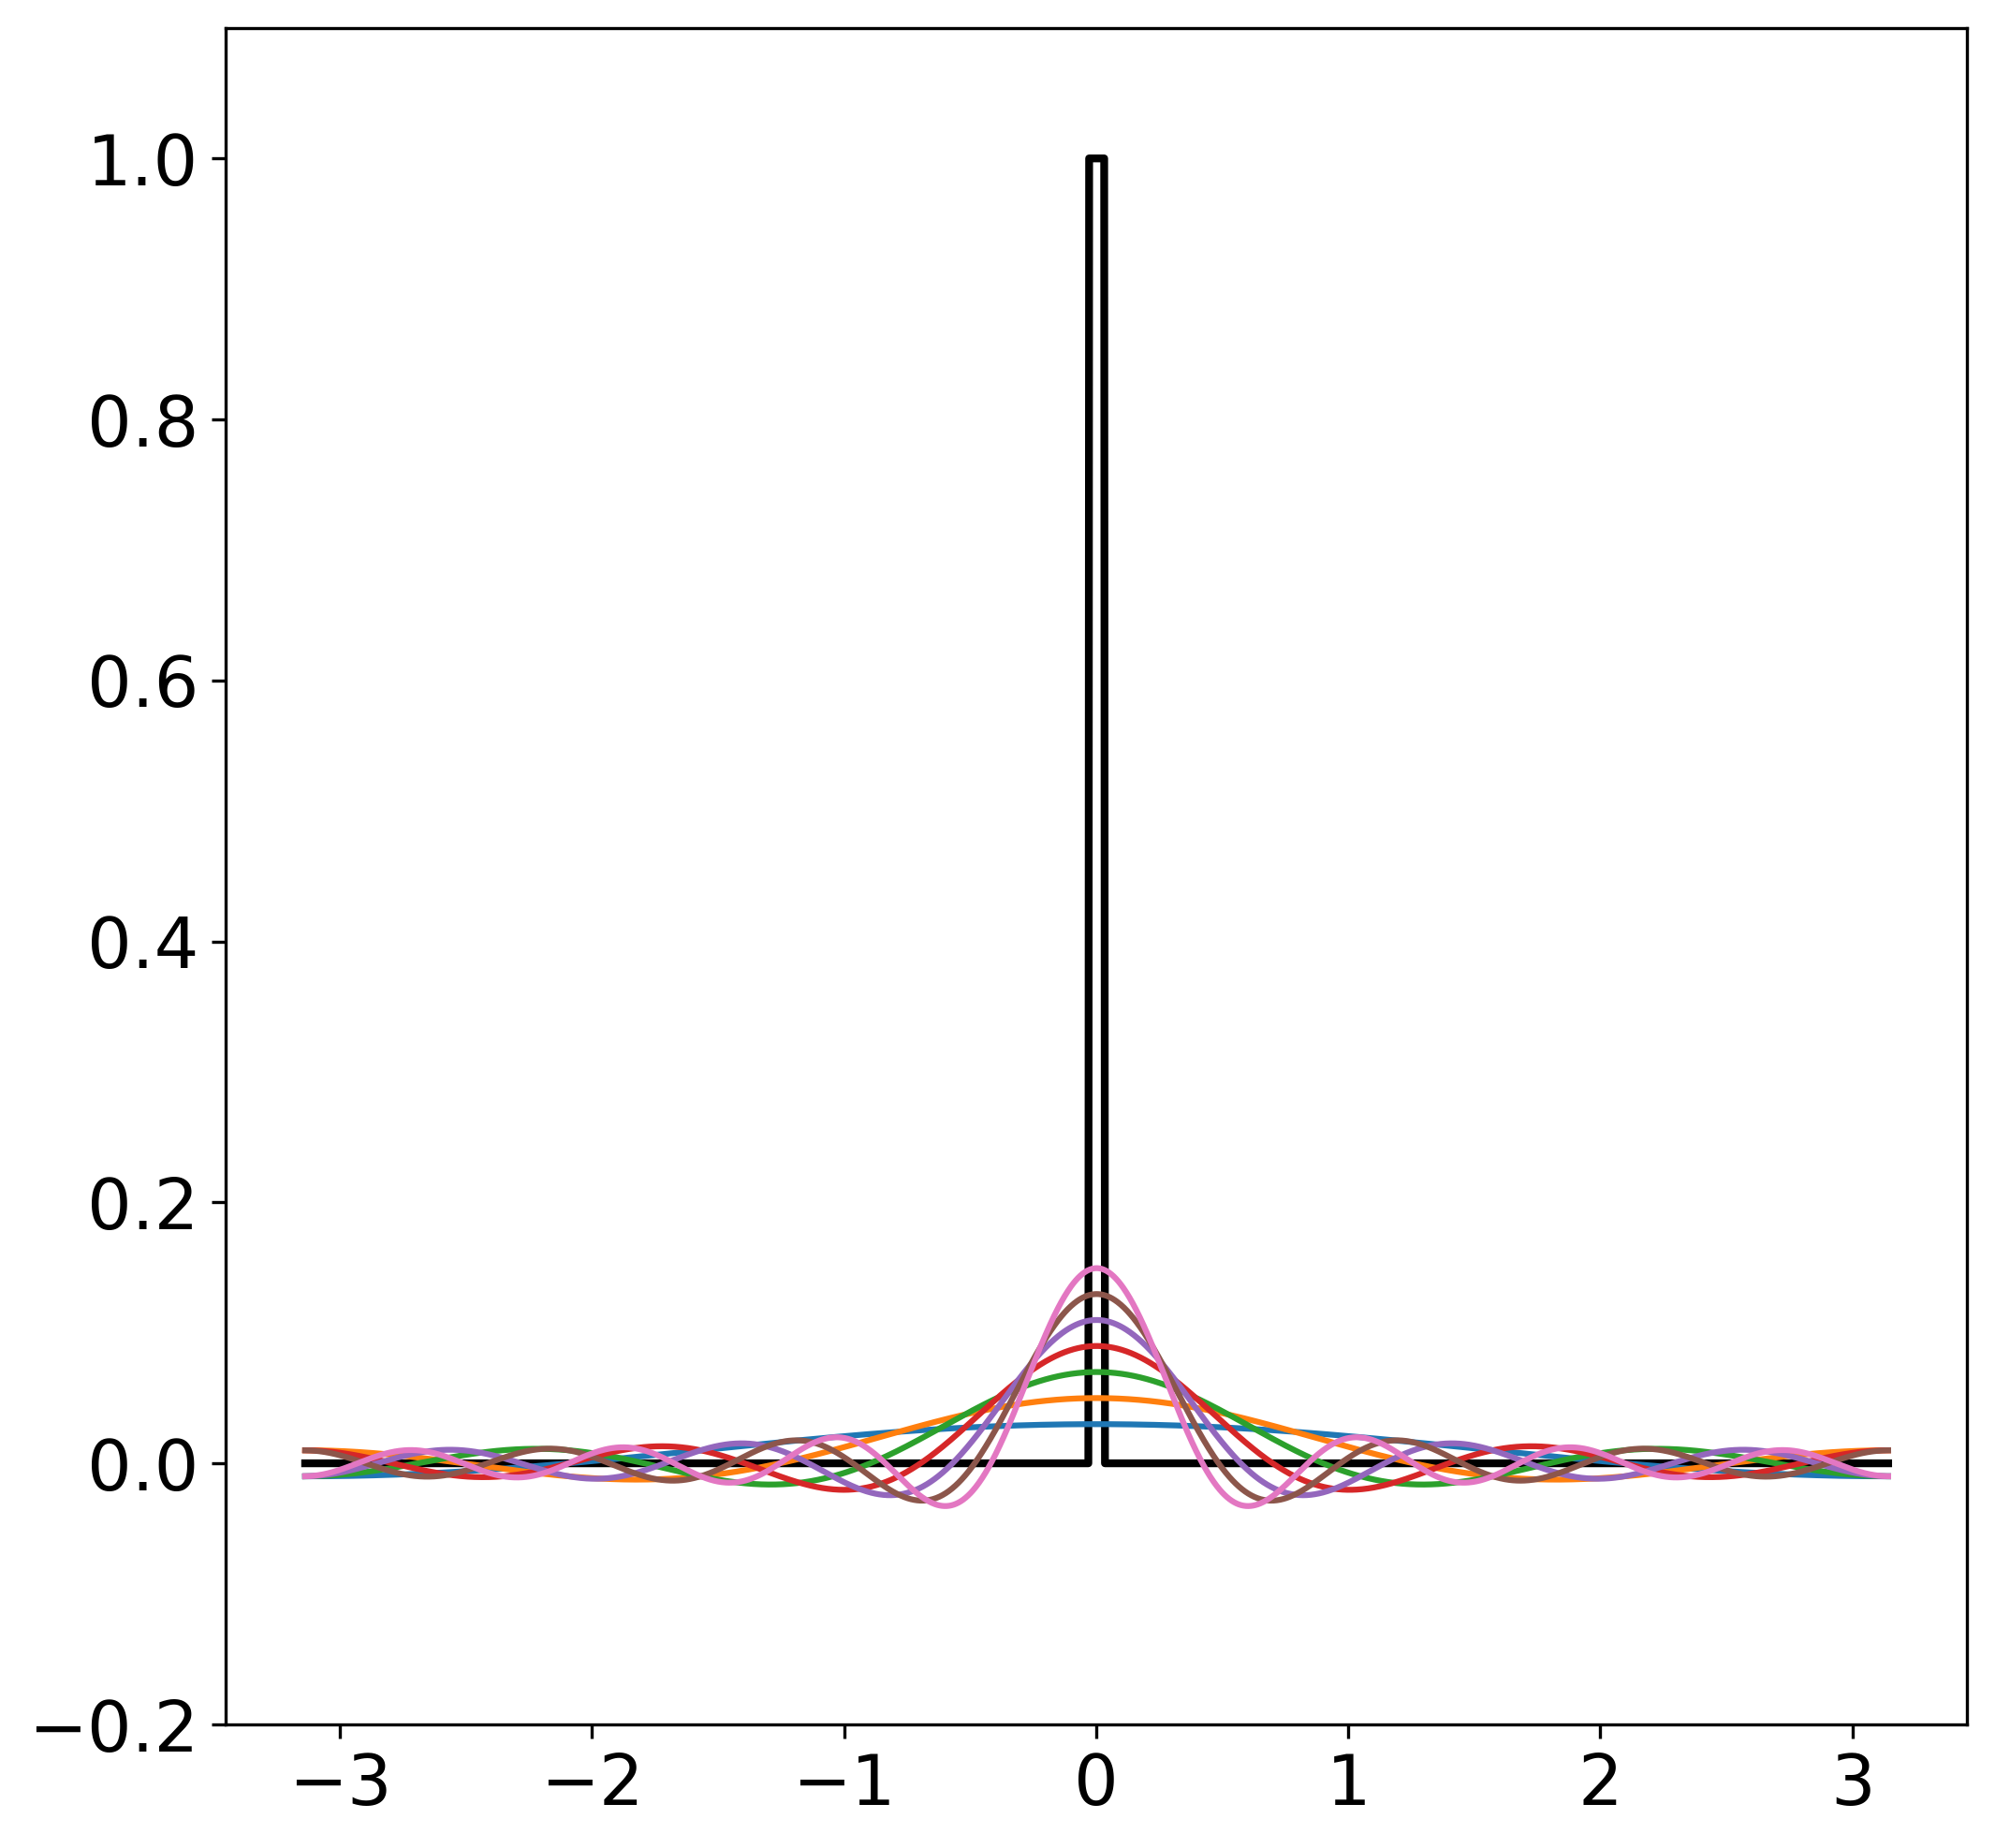
\includegraphics[width=.5\linewidth]{programs/fourier2/out_7.png}}
    \only<9|handout:0>{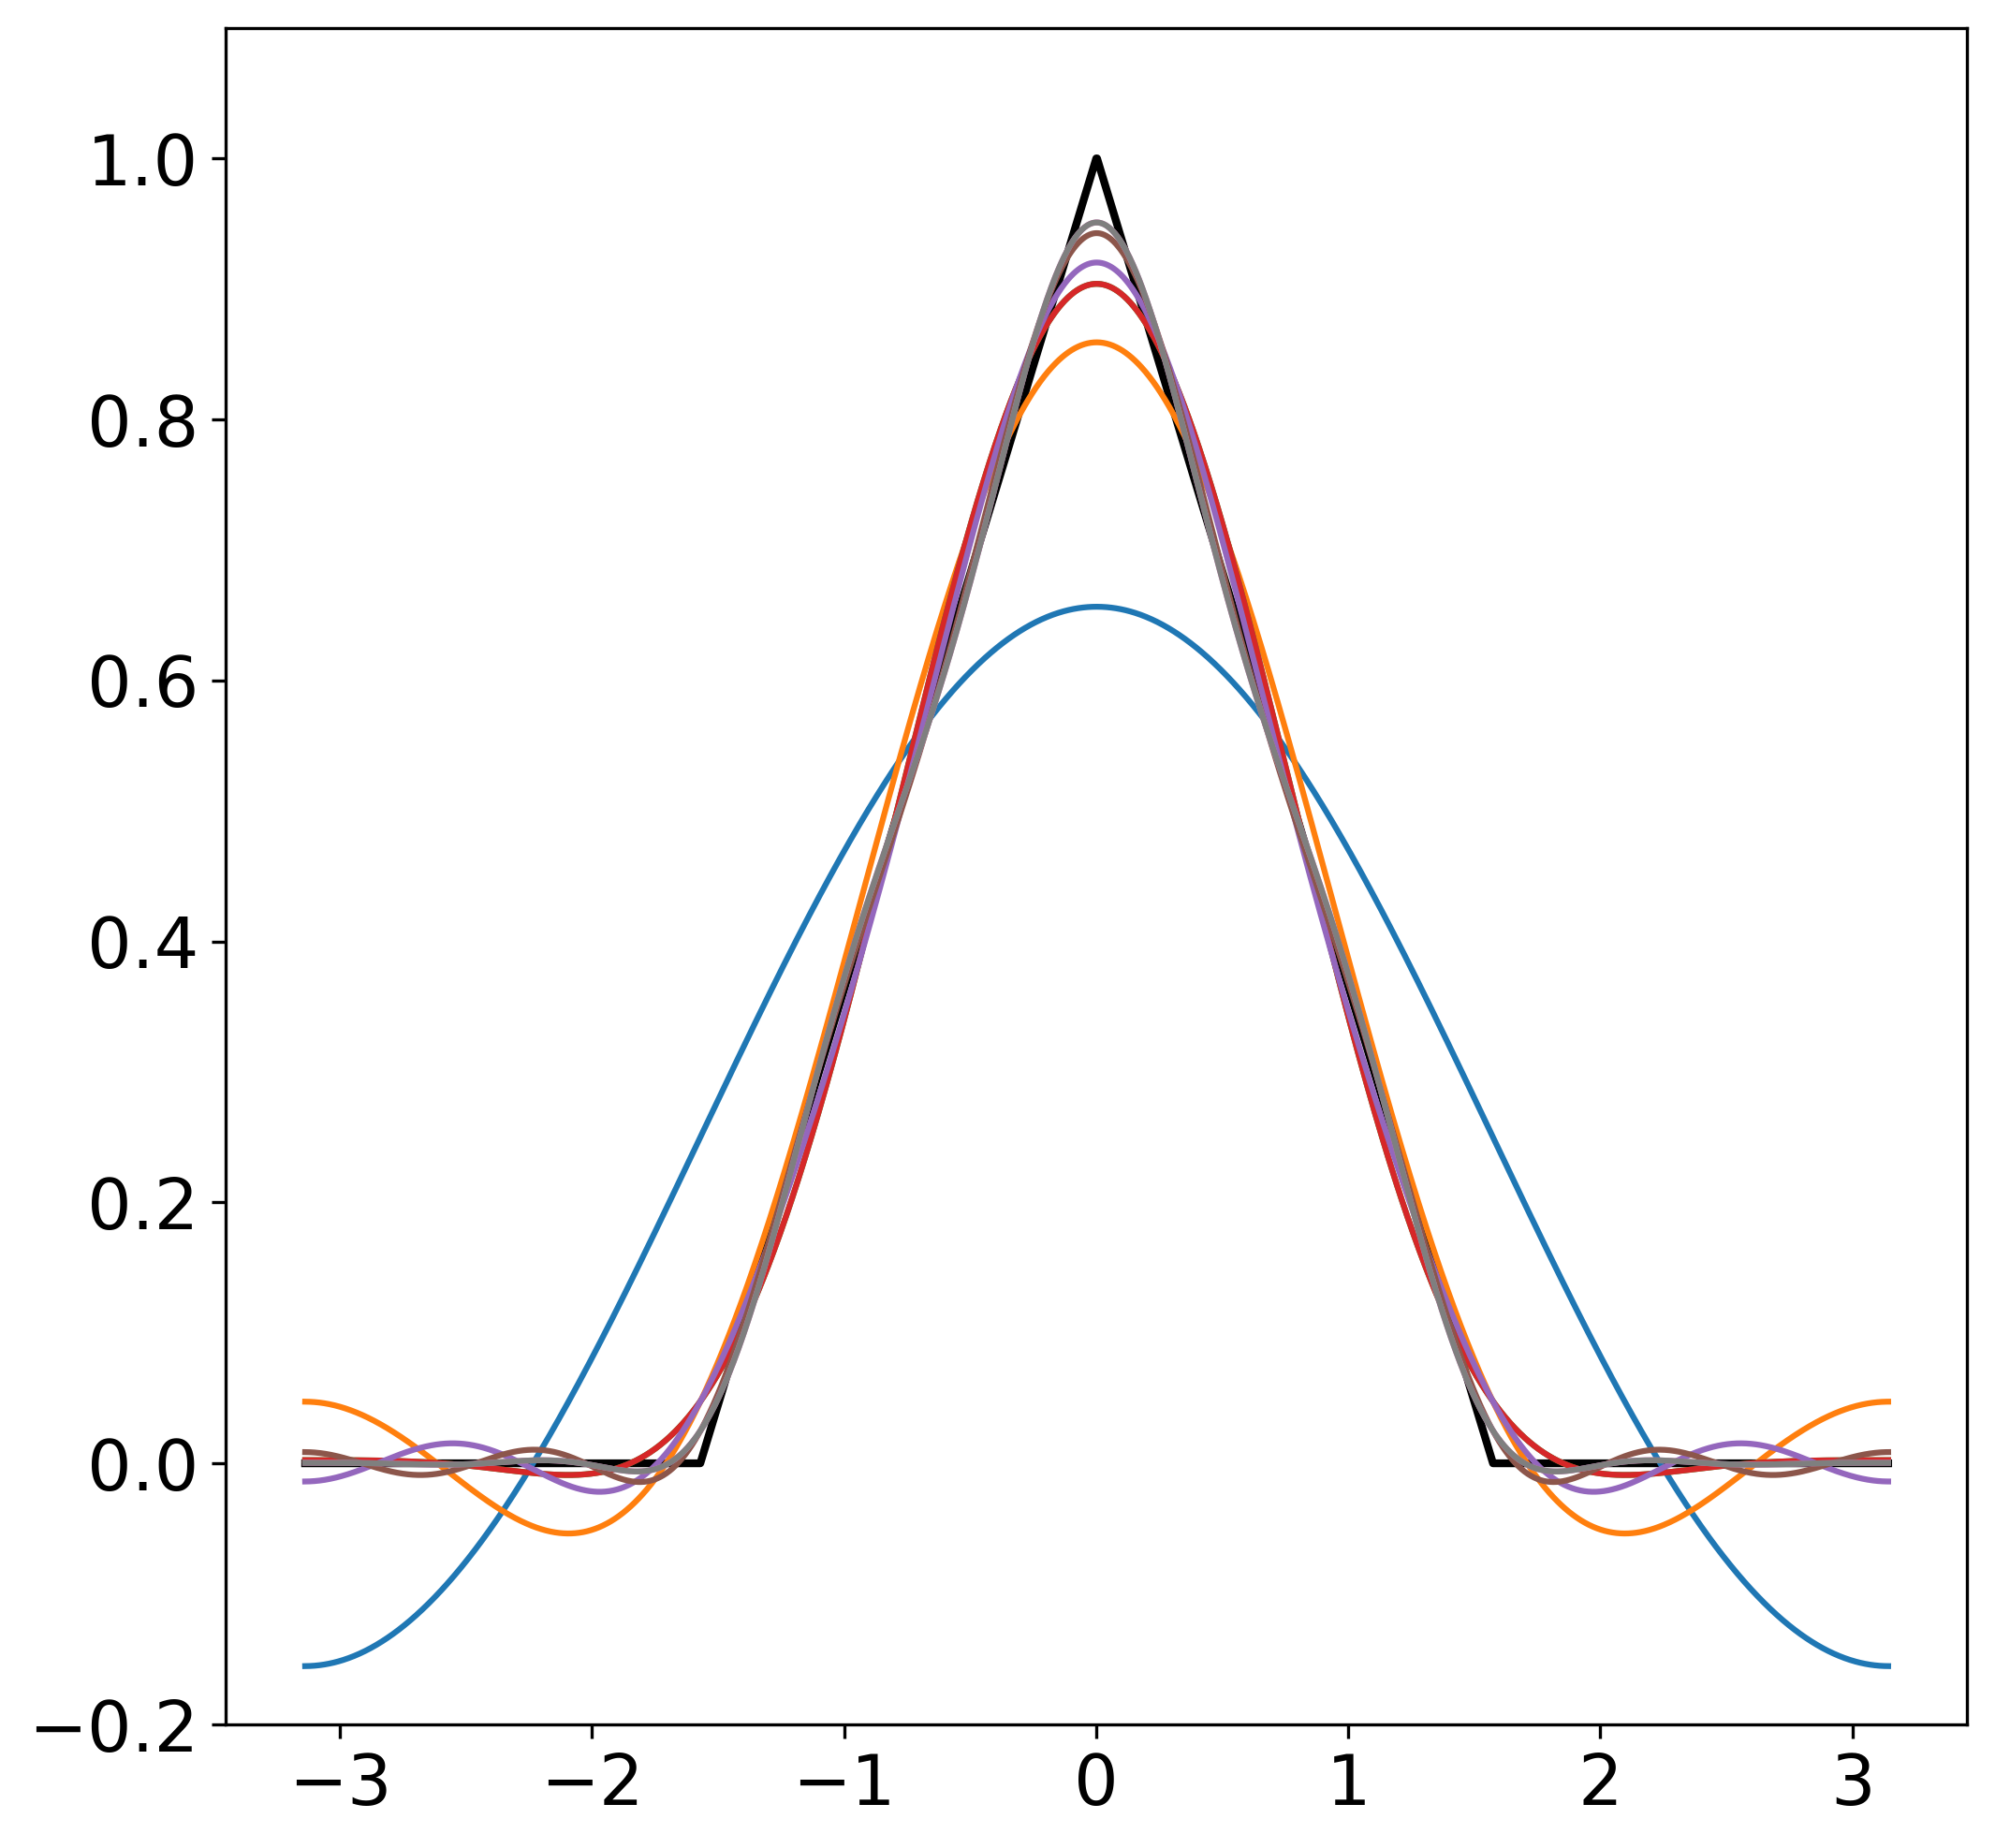
\includegraphics[width=.5\linewidth]{programs/fourier1/out_8.png}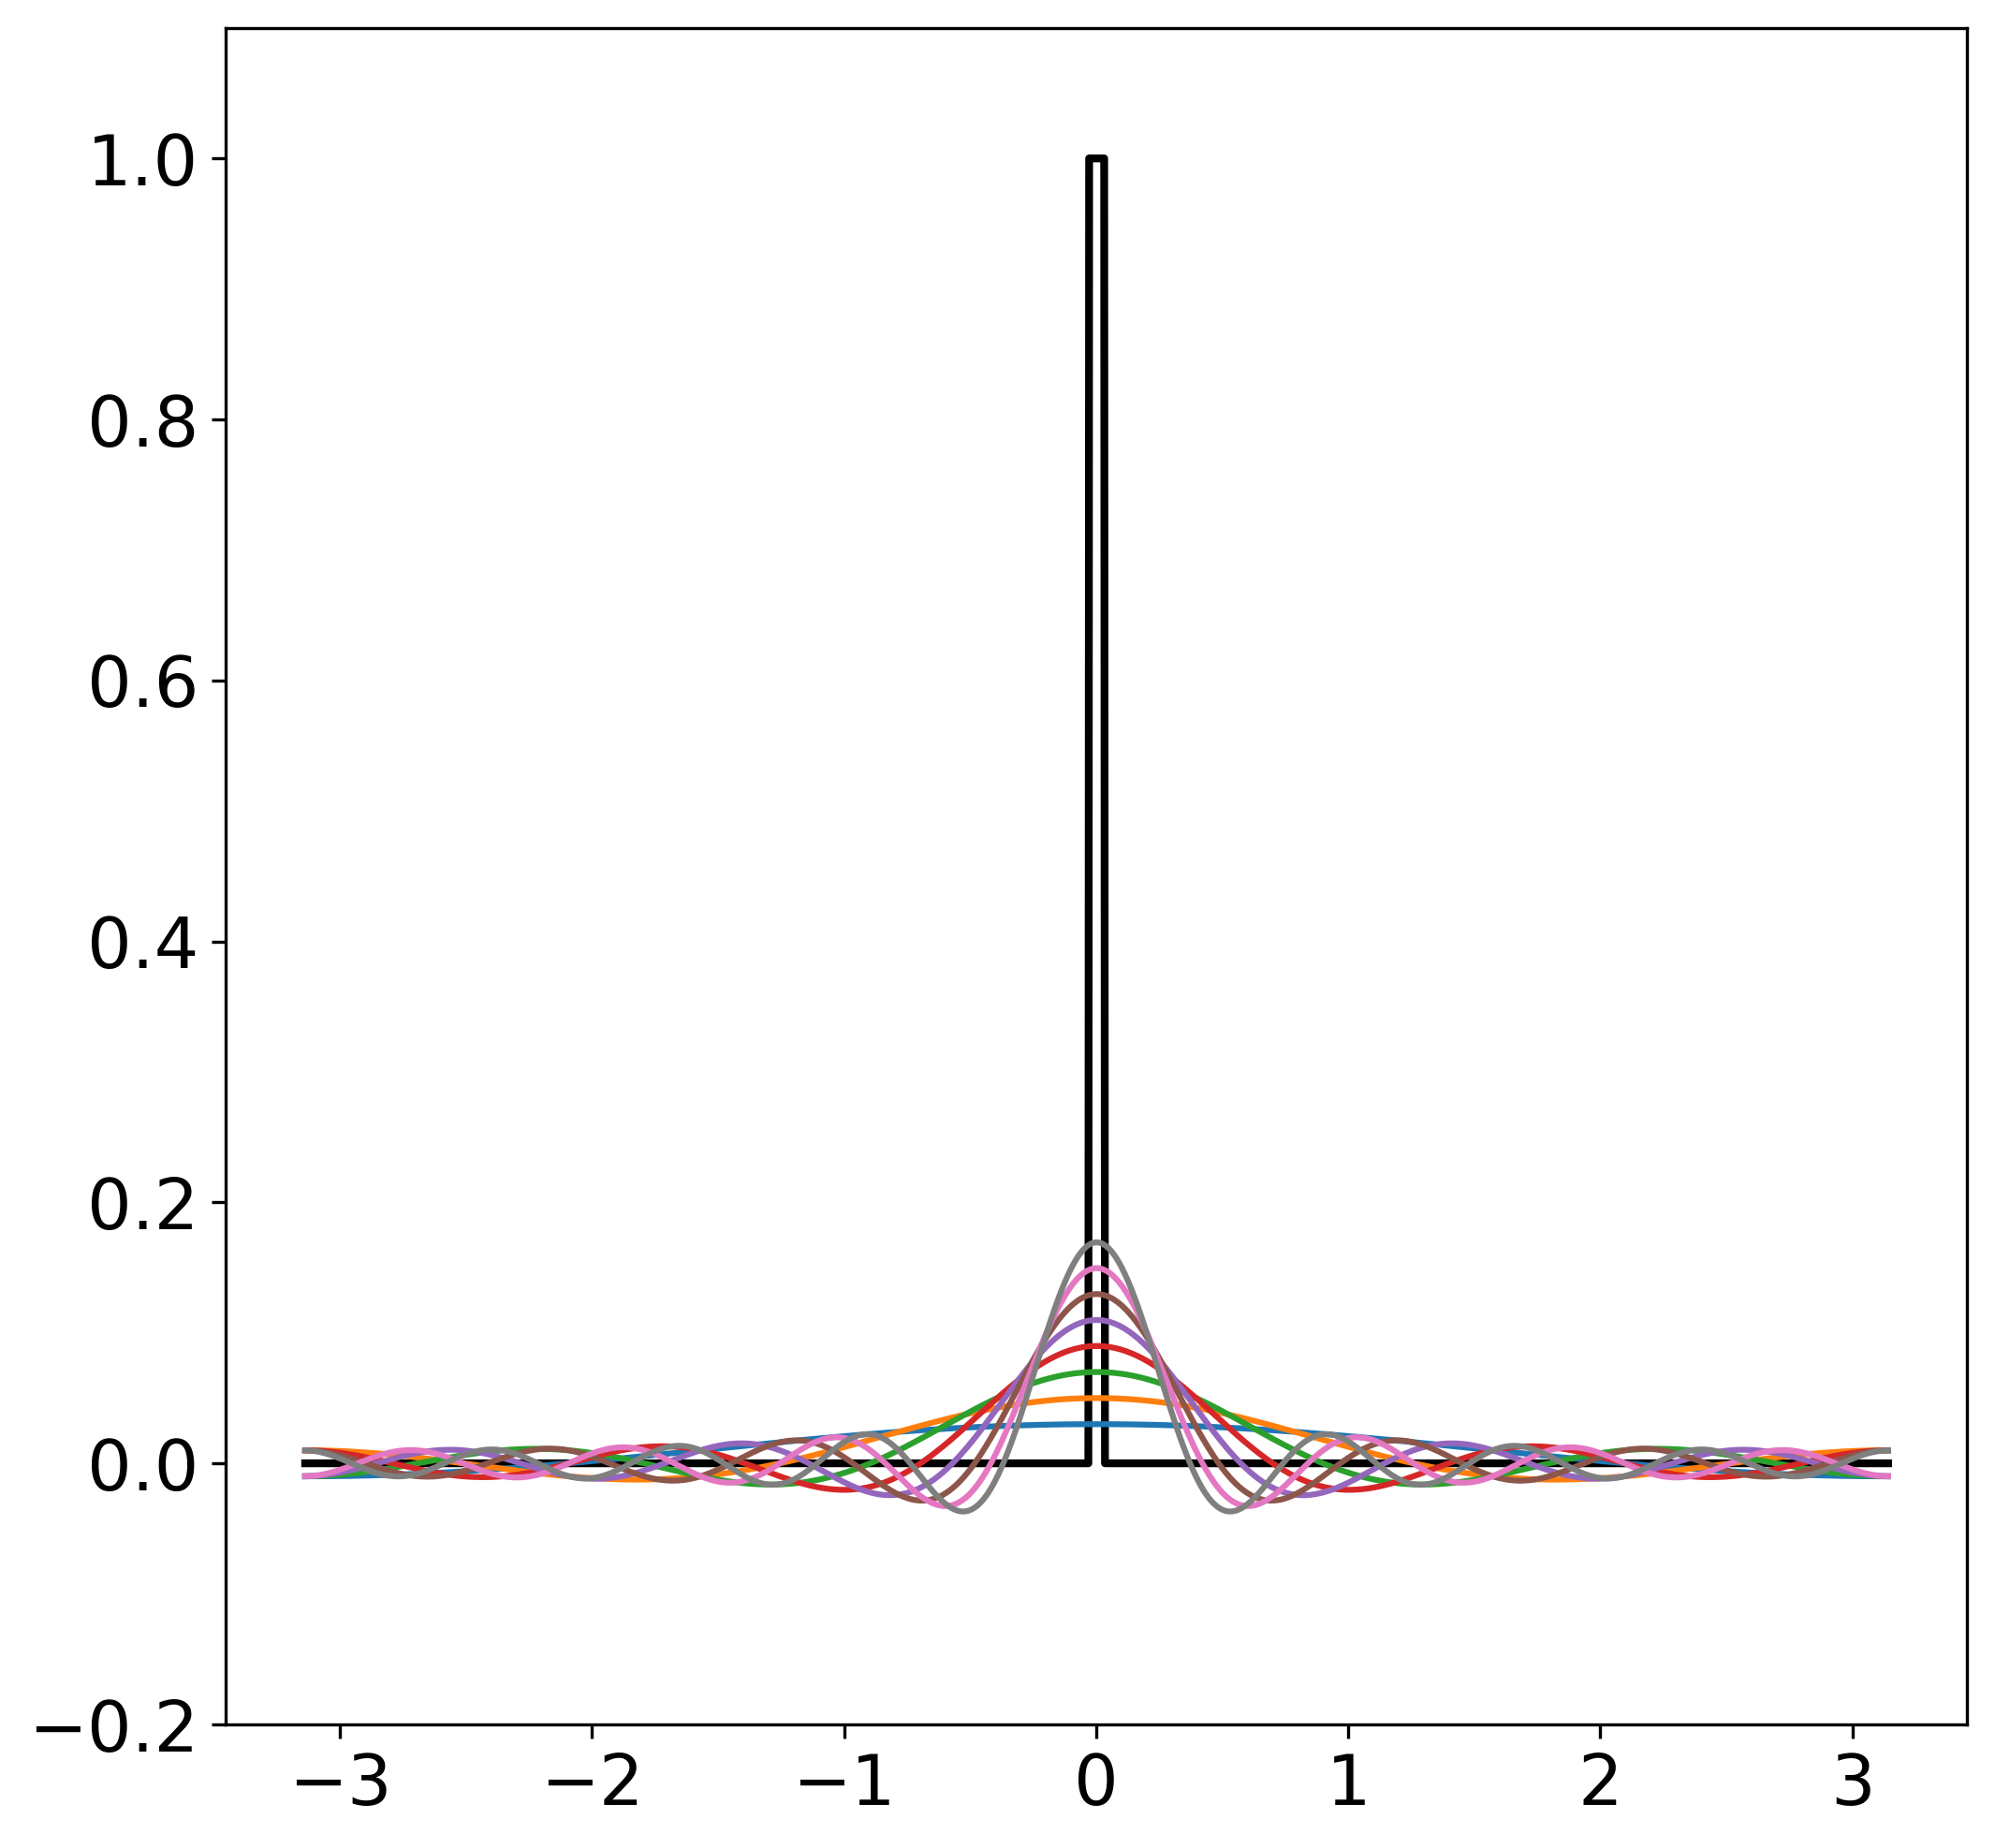
\includegraphics[width=.5\linewidth]{programs/fourier2/out_8.png}}
    \only<10|handout:0>{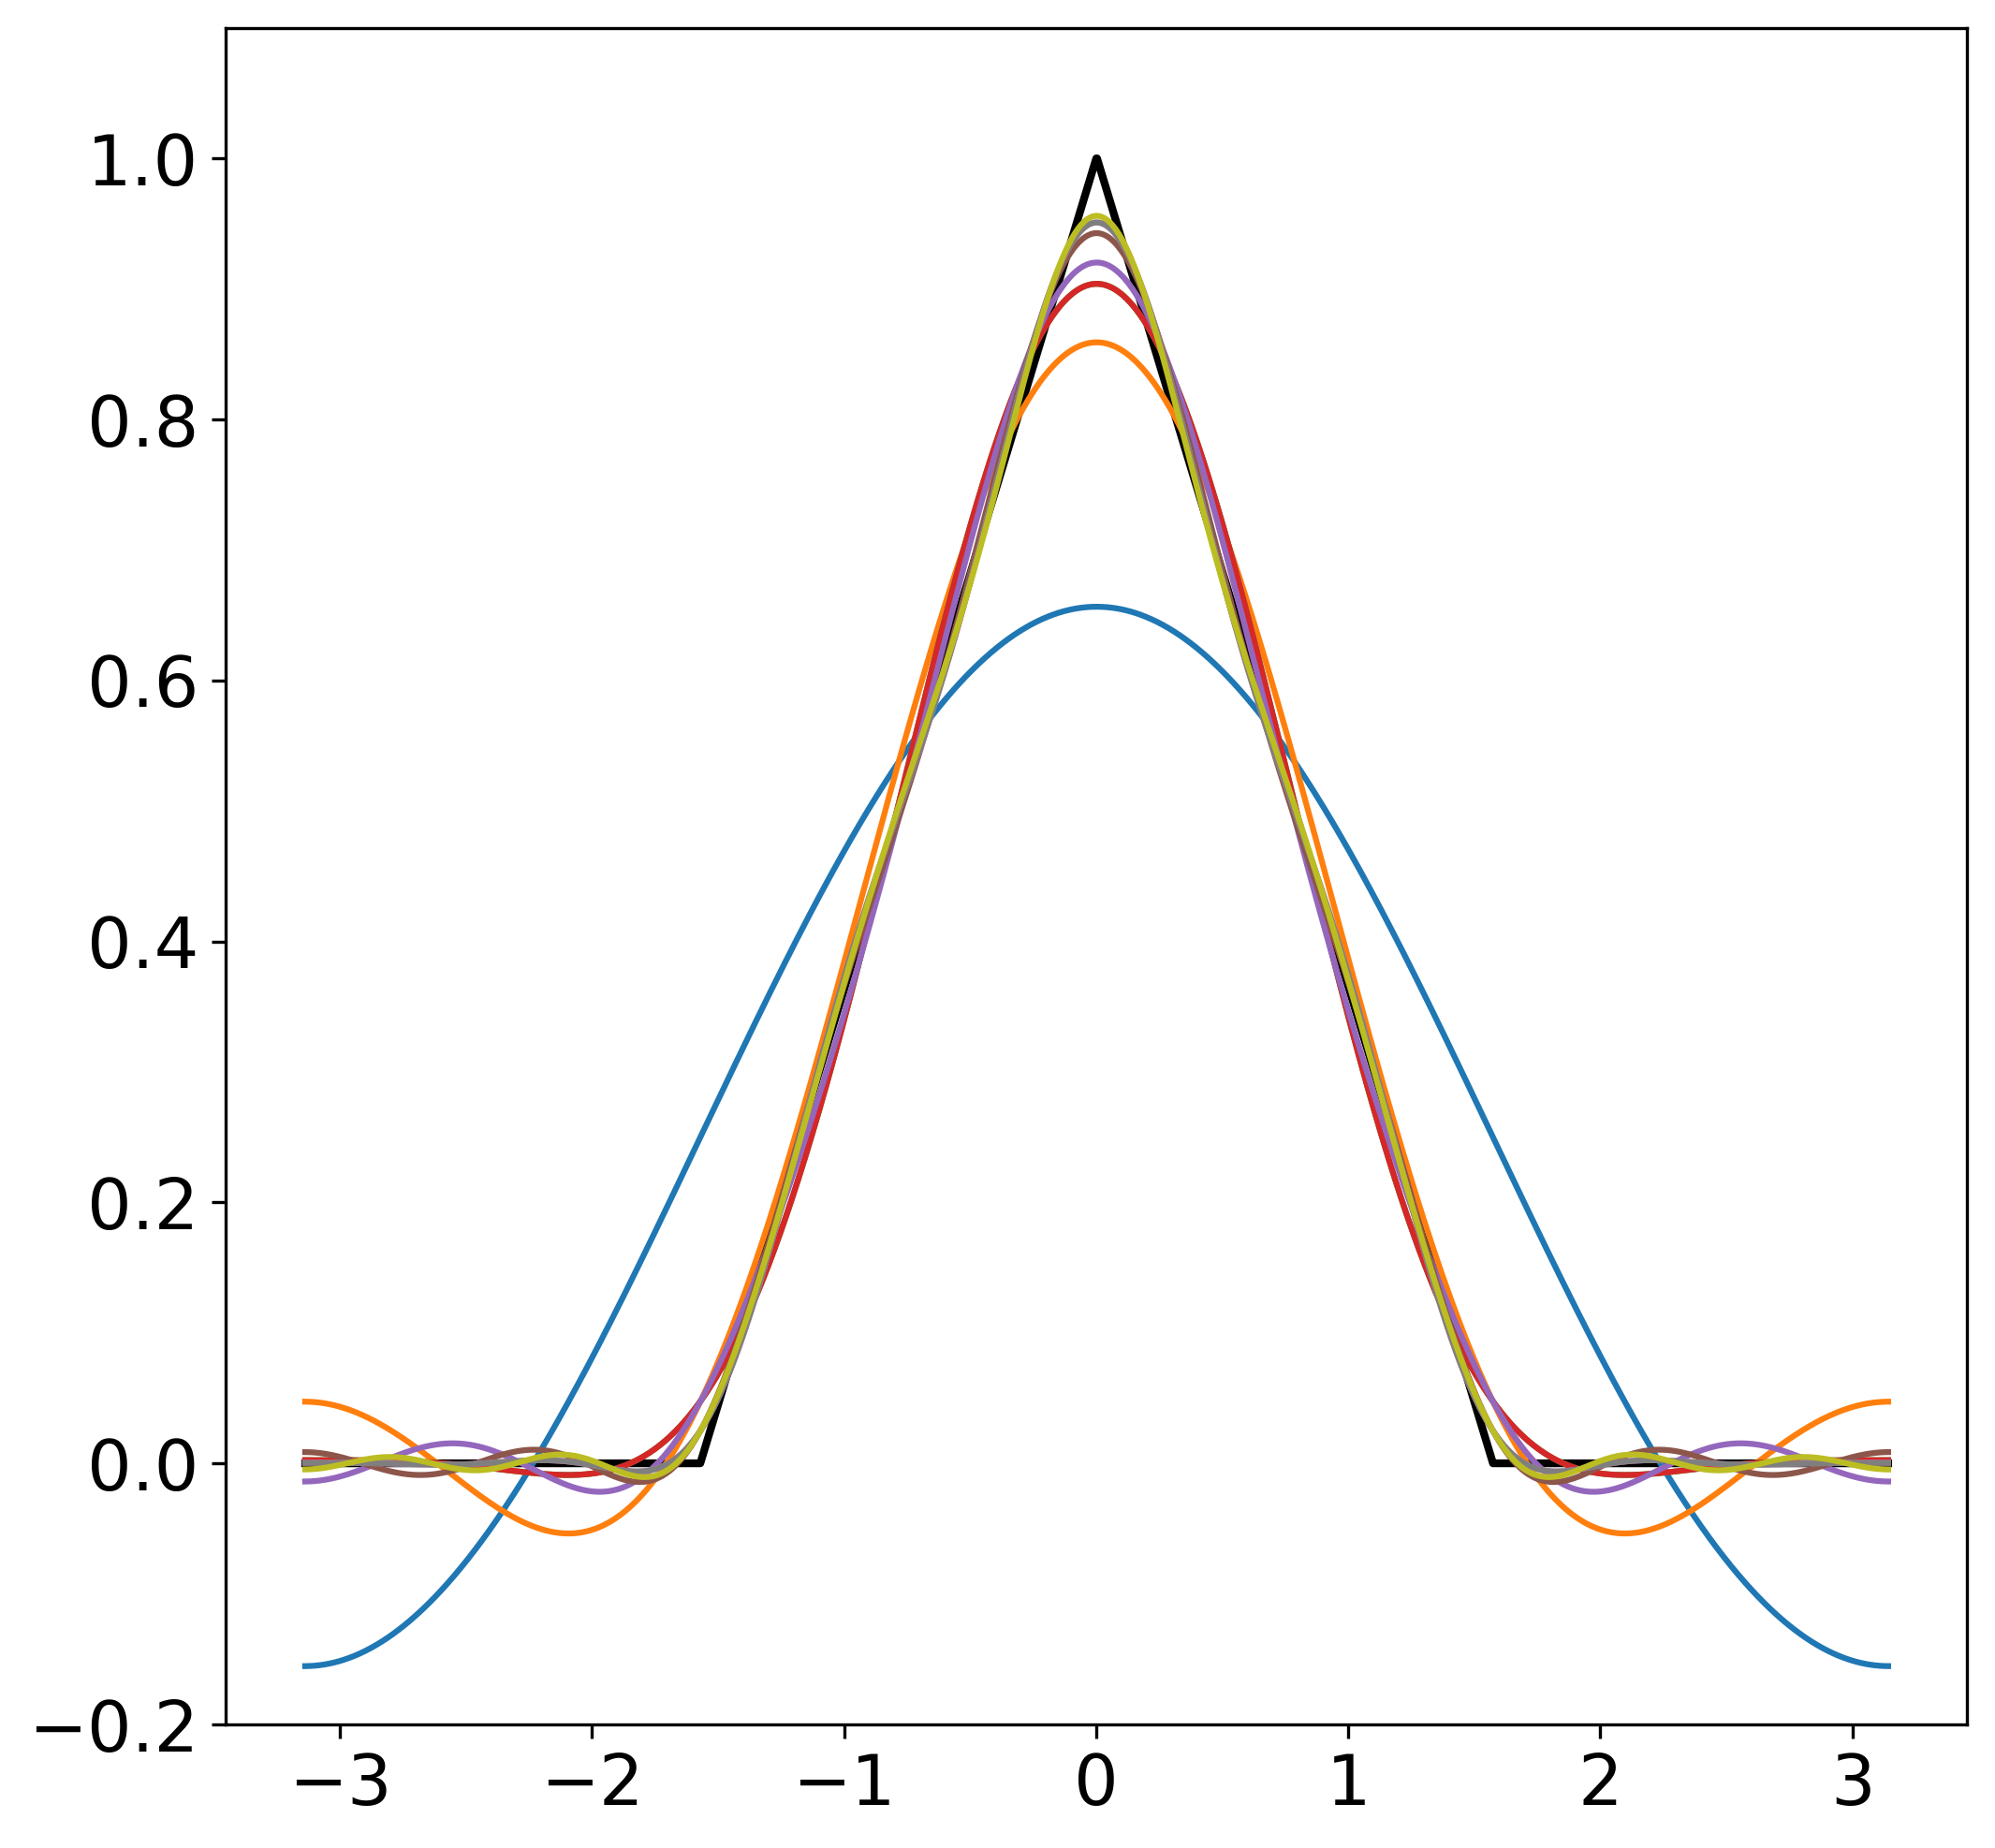
\includegraphics[width=.5\linewidth]{programs/fourier1/out_9.png}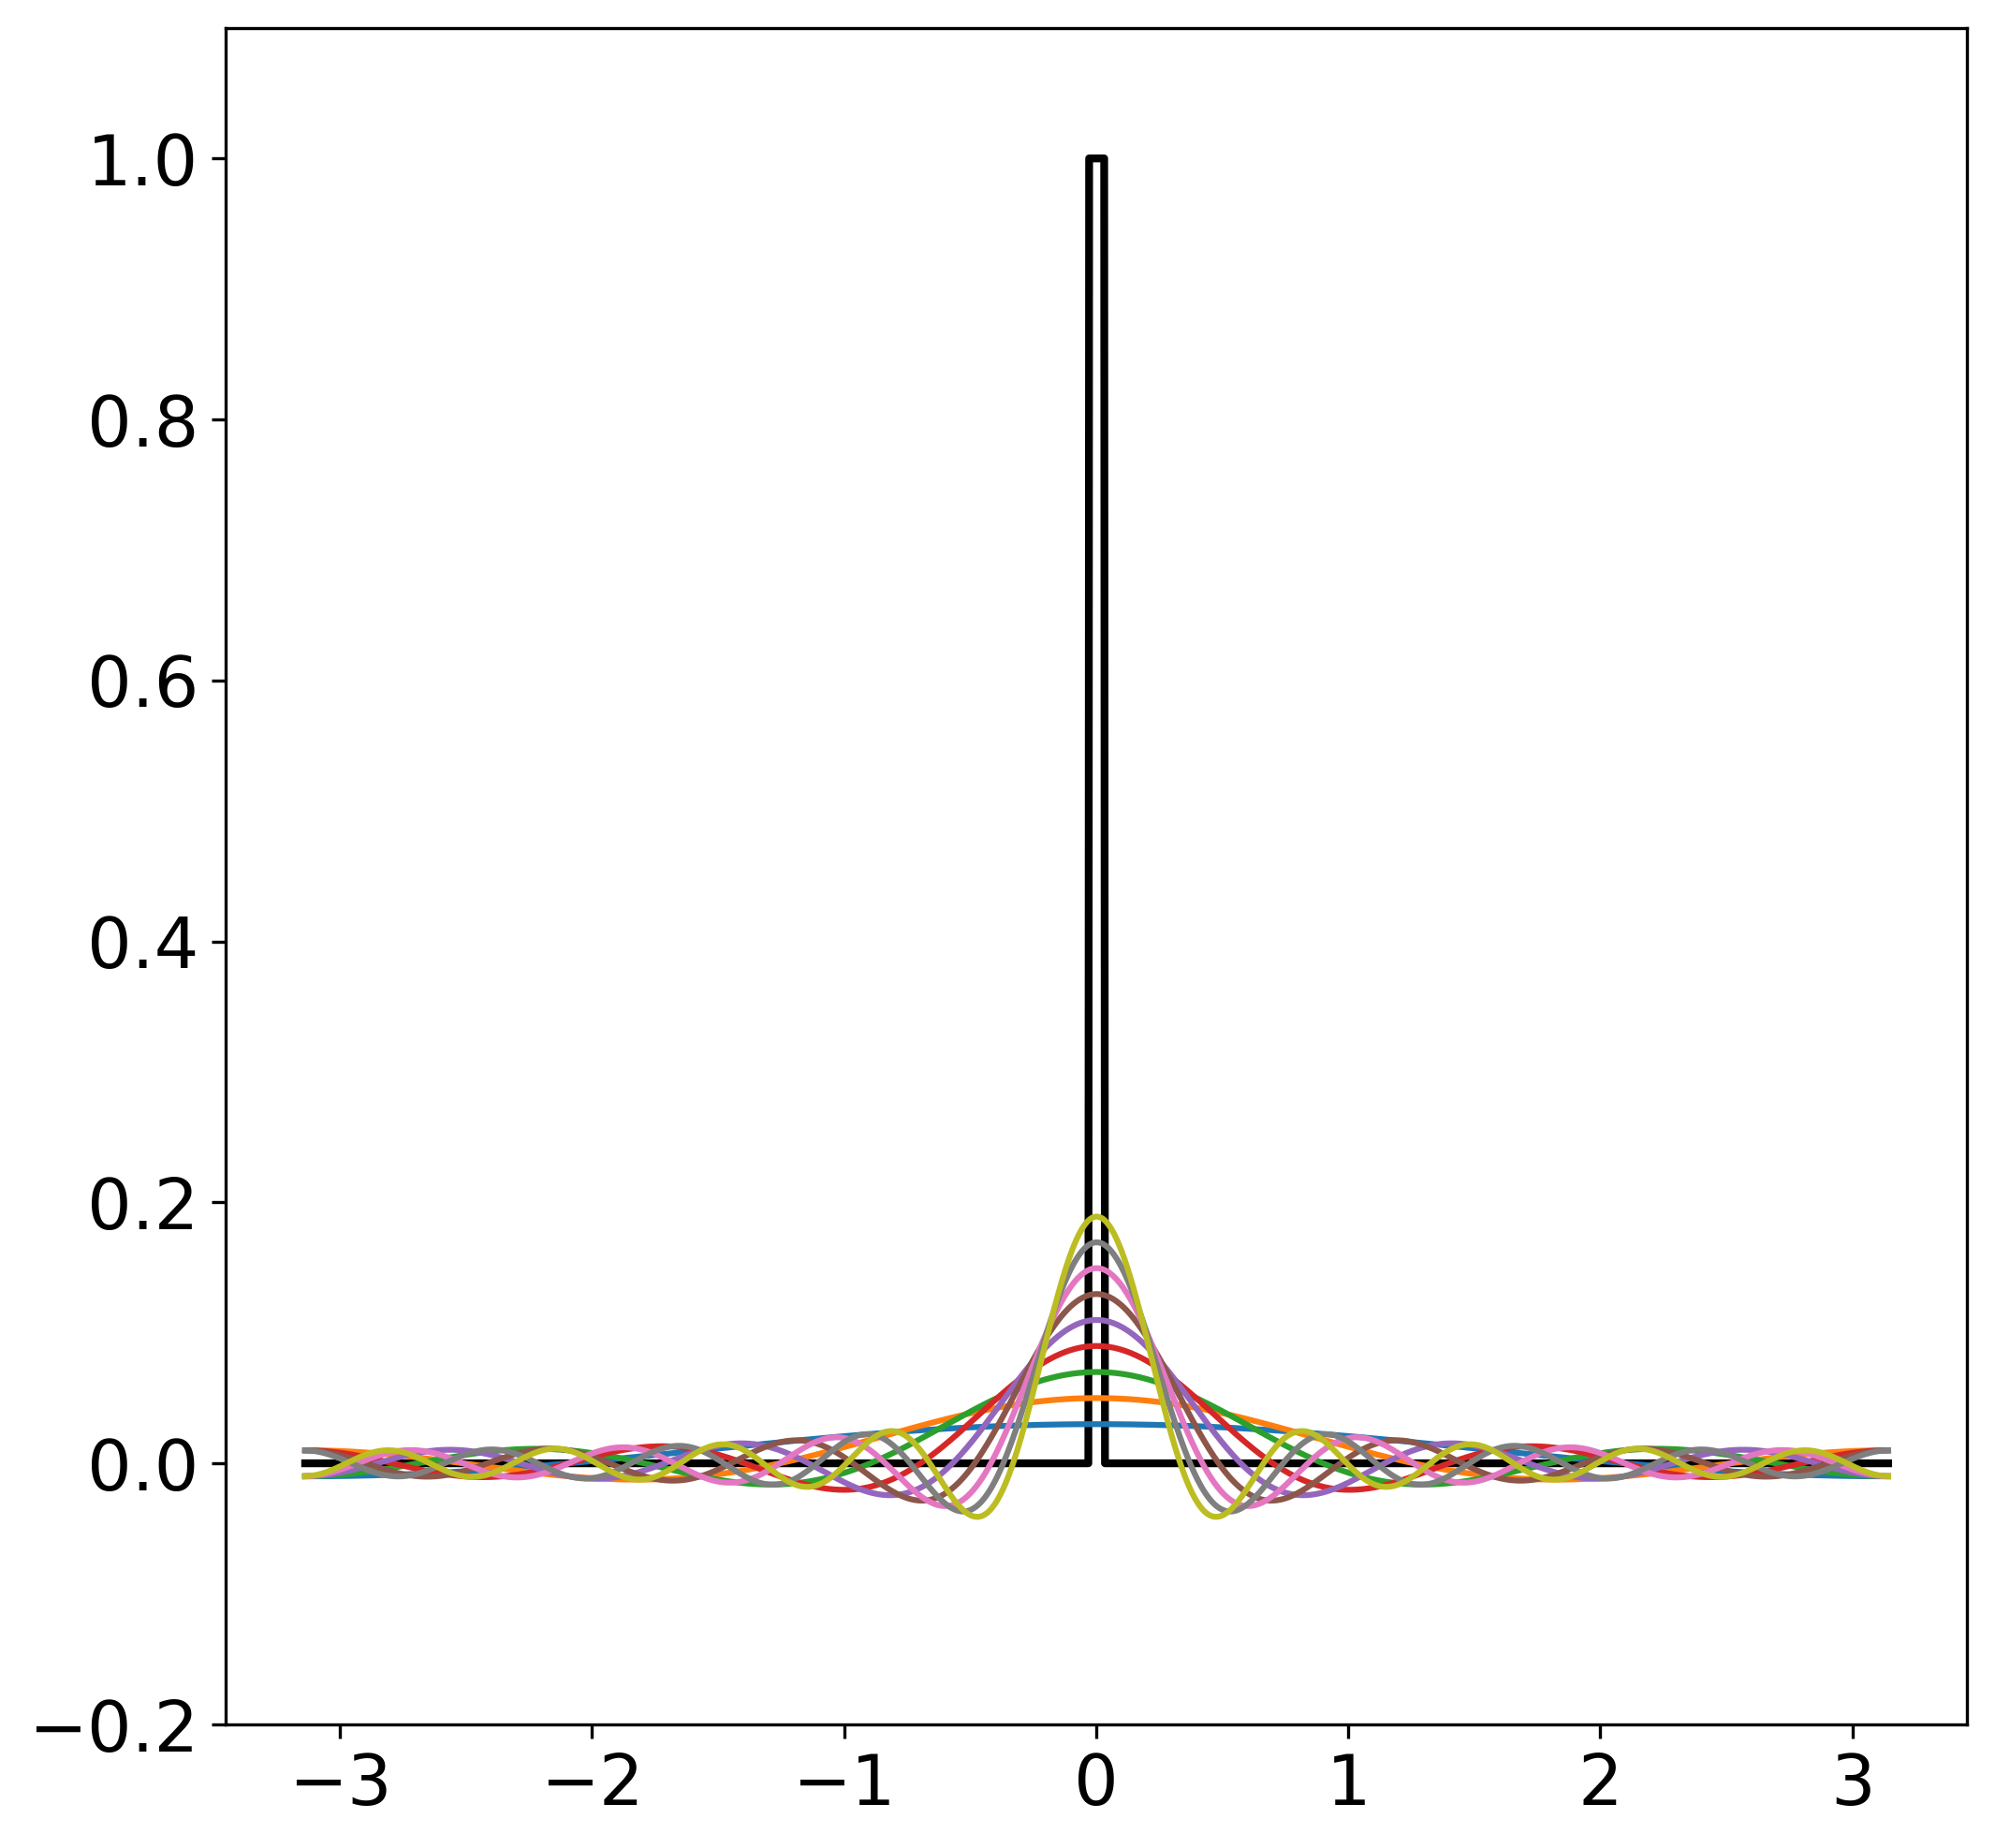
\includegraphics[width=.5\linewidth]{programs/fourier2/out_9.png}}
    \only<11|handout:0>{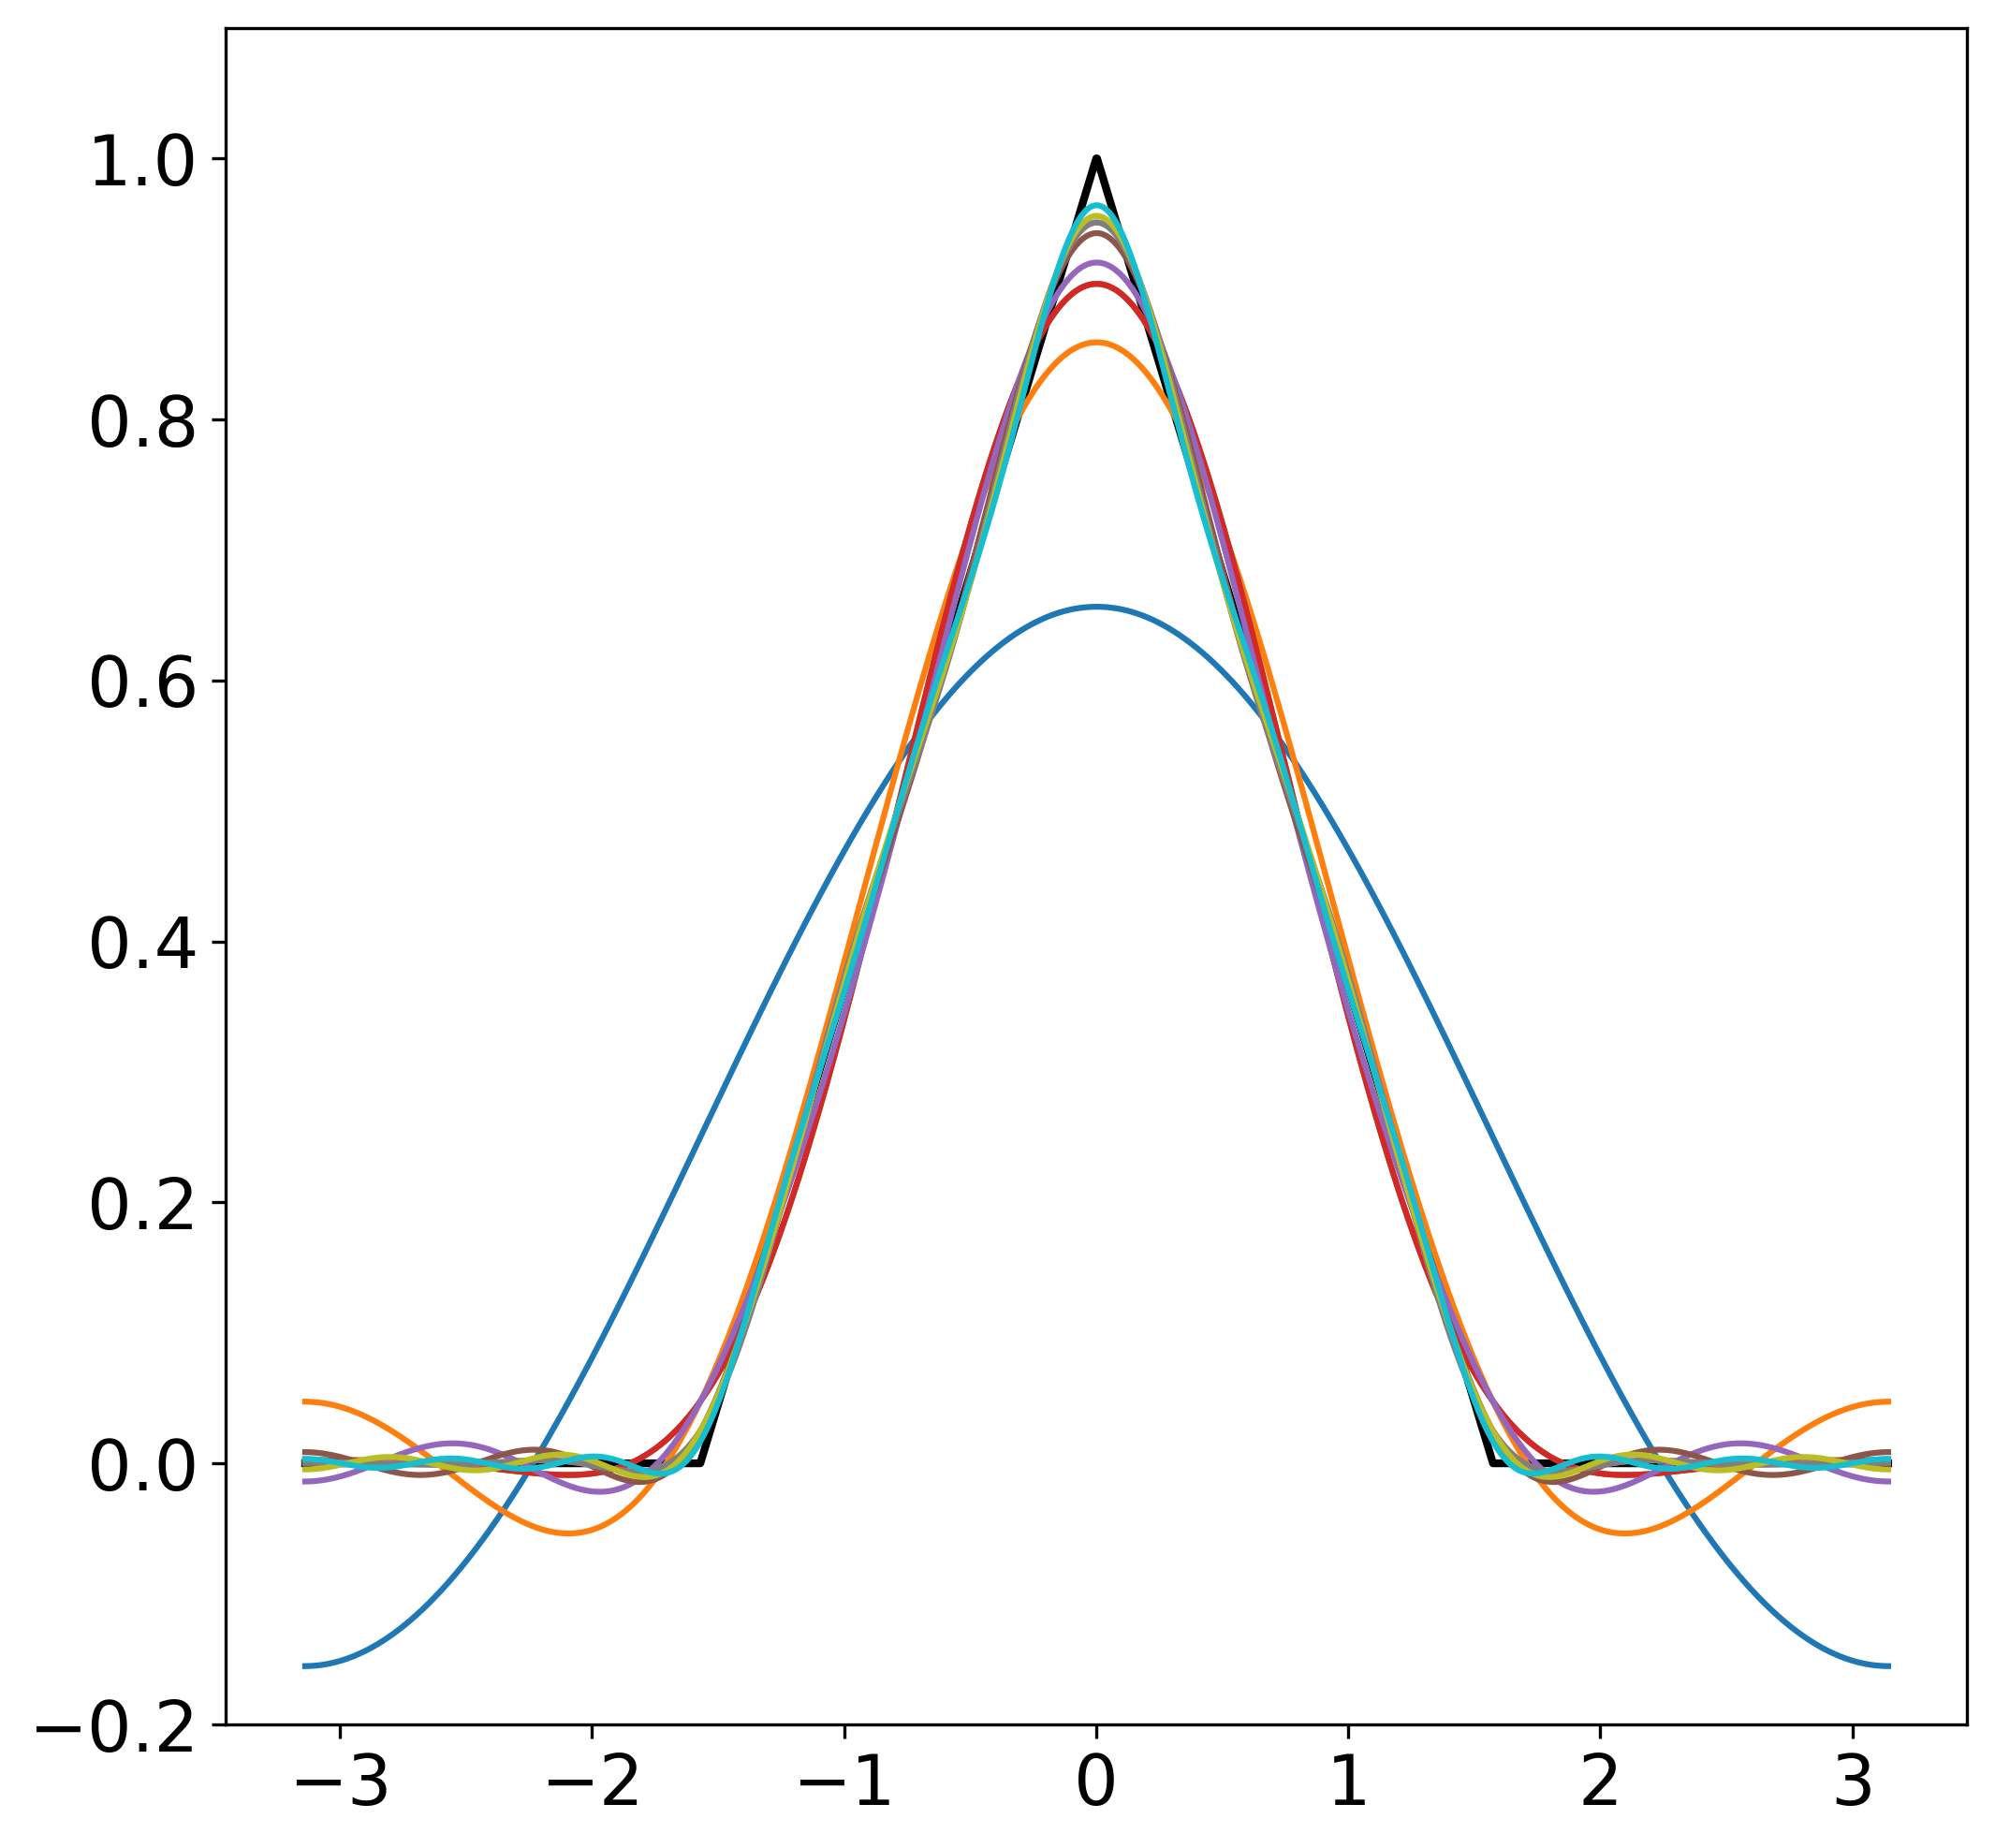
\includegraphics[width=.5\linewidth]{programs/fourier1/out_10.png}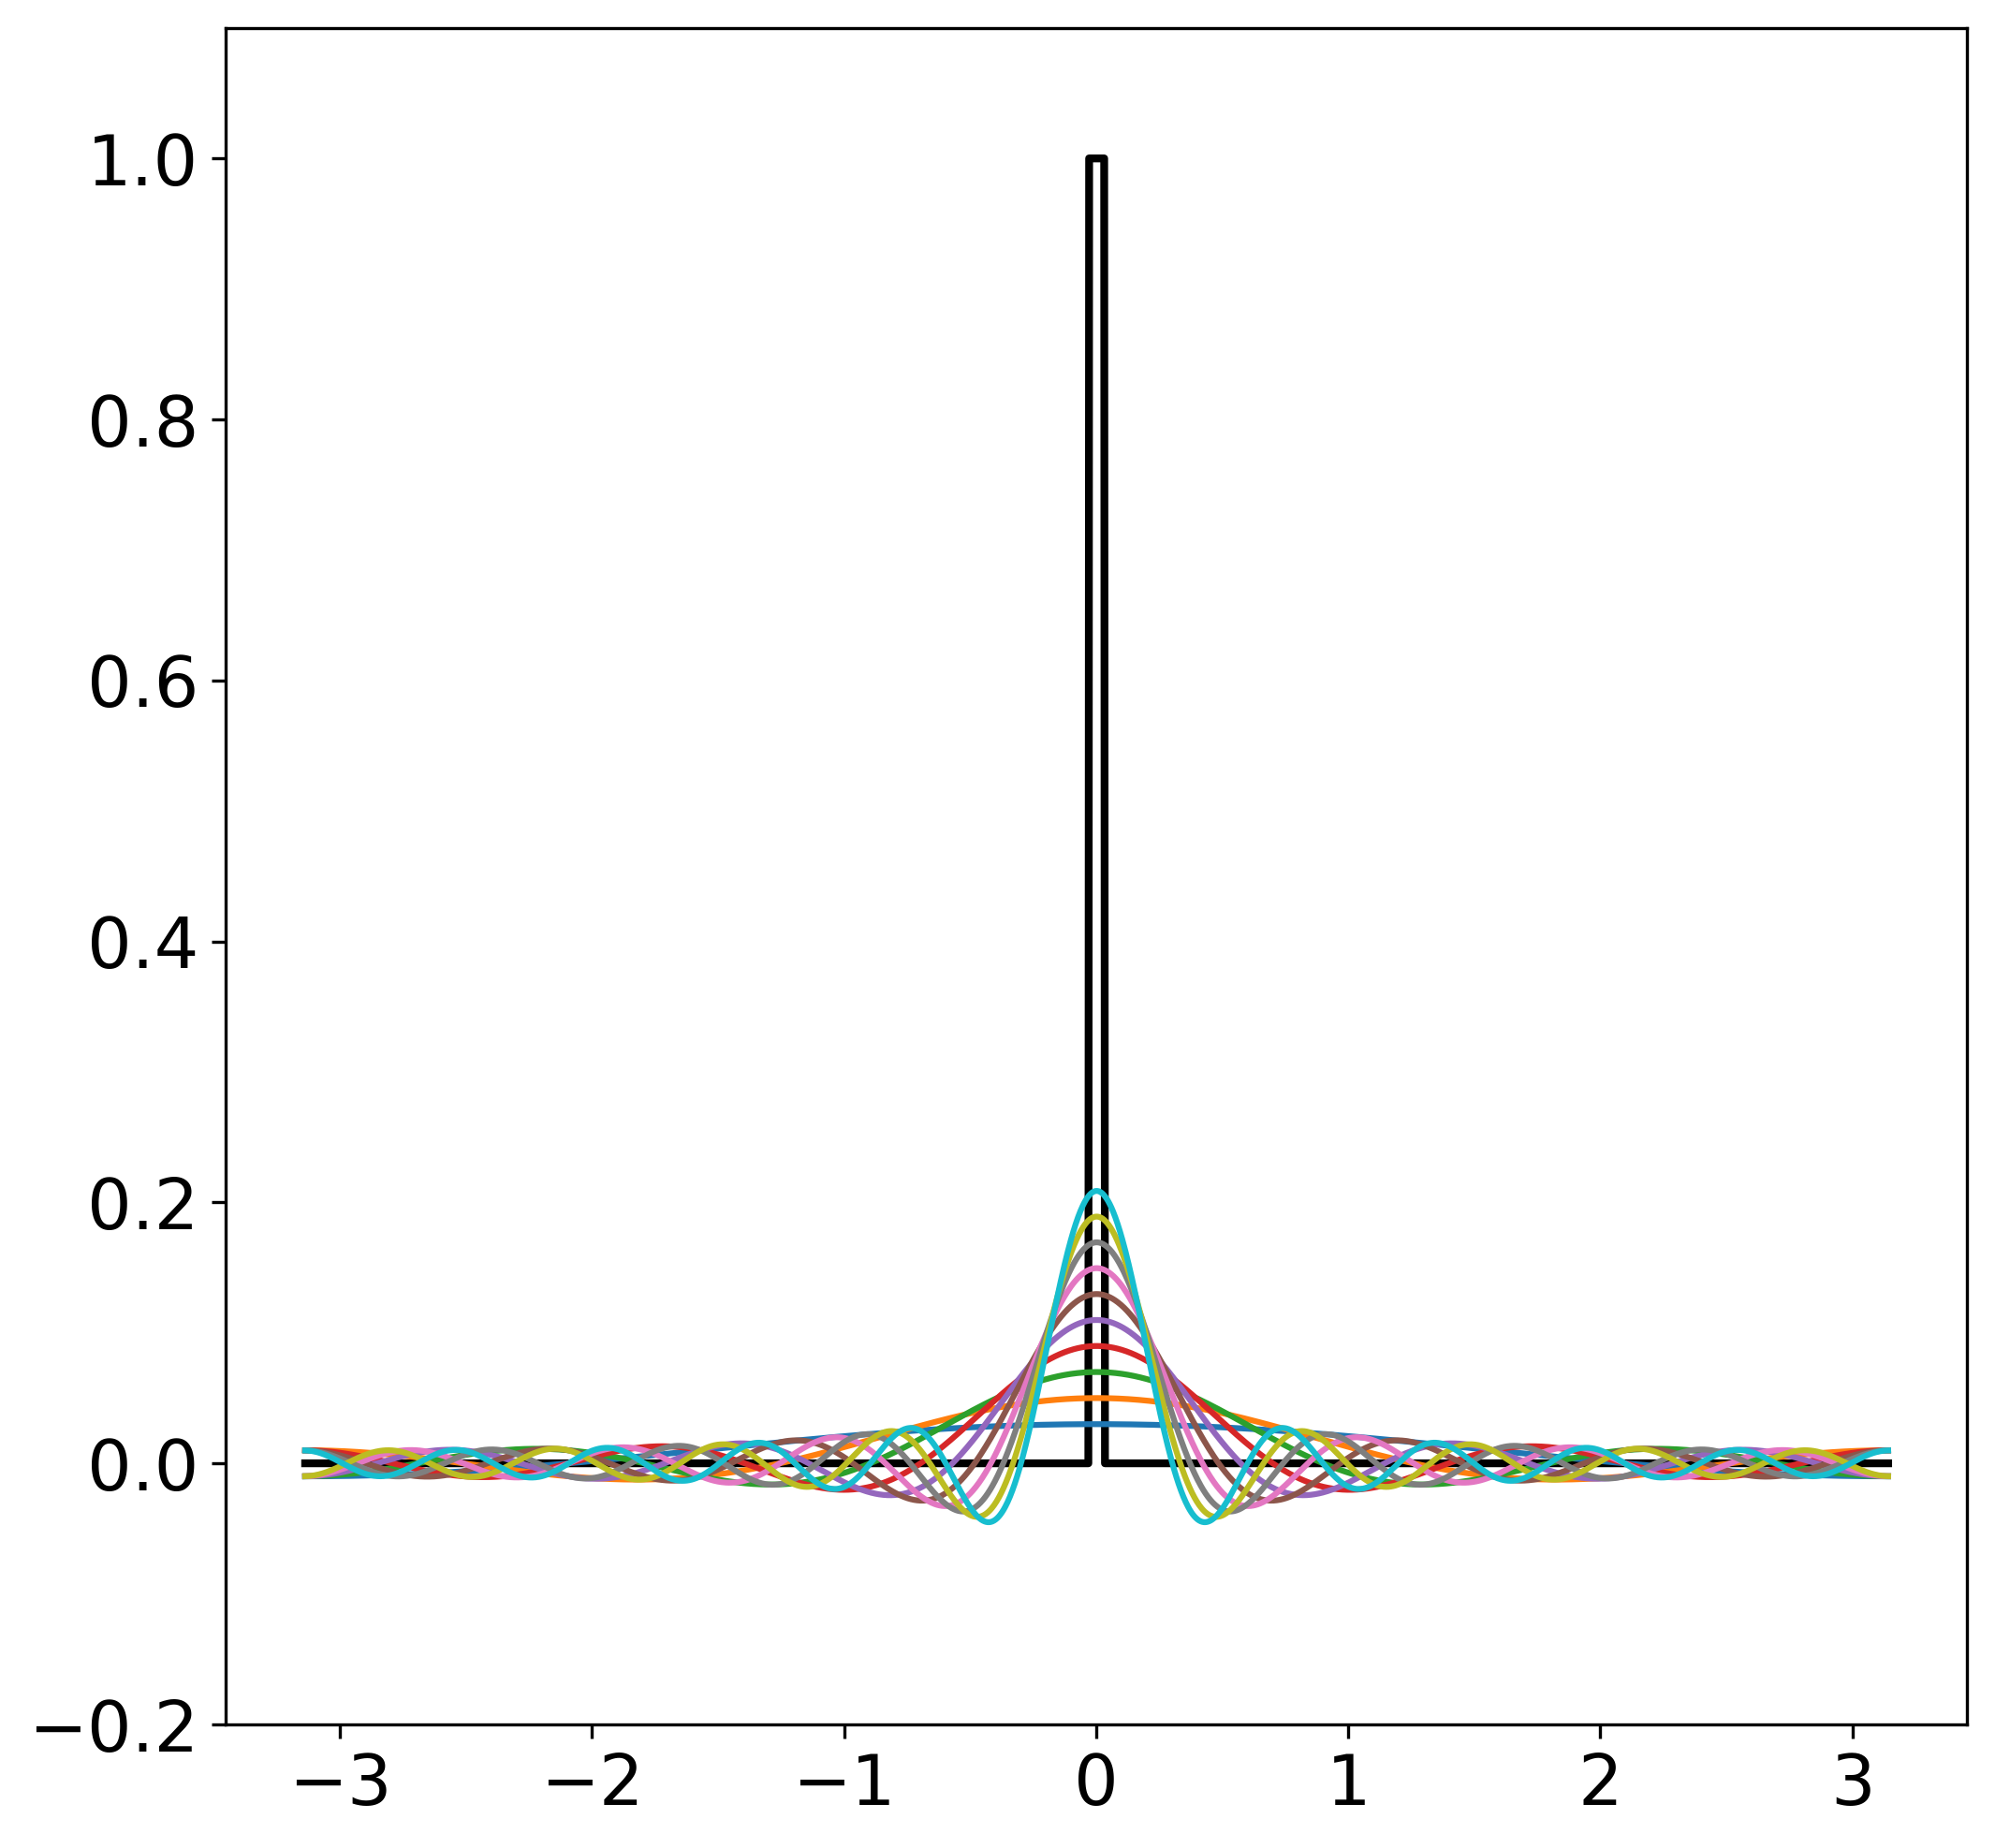
\includegraphics[width=.5\linewidth]{programs/fourier2/out_10.png}}
    \only<12|handout:0>{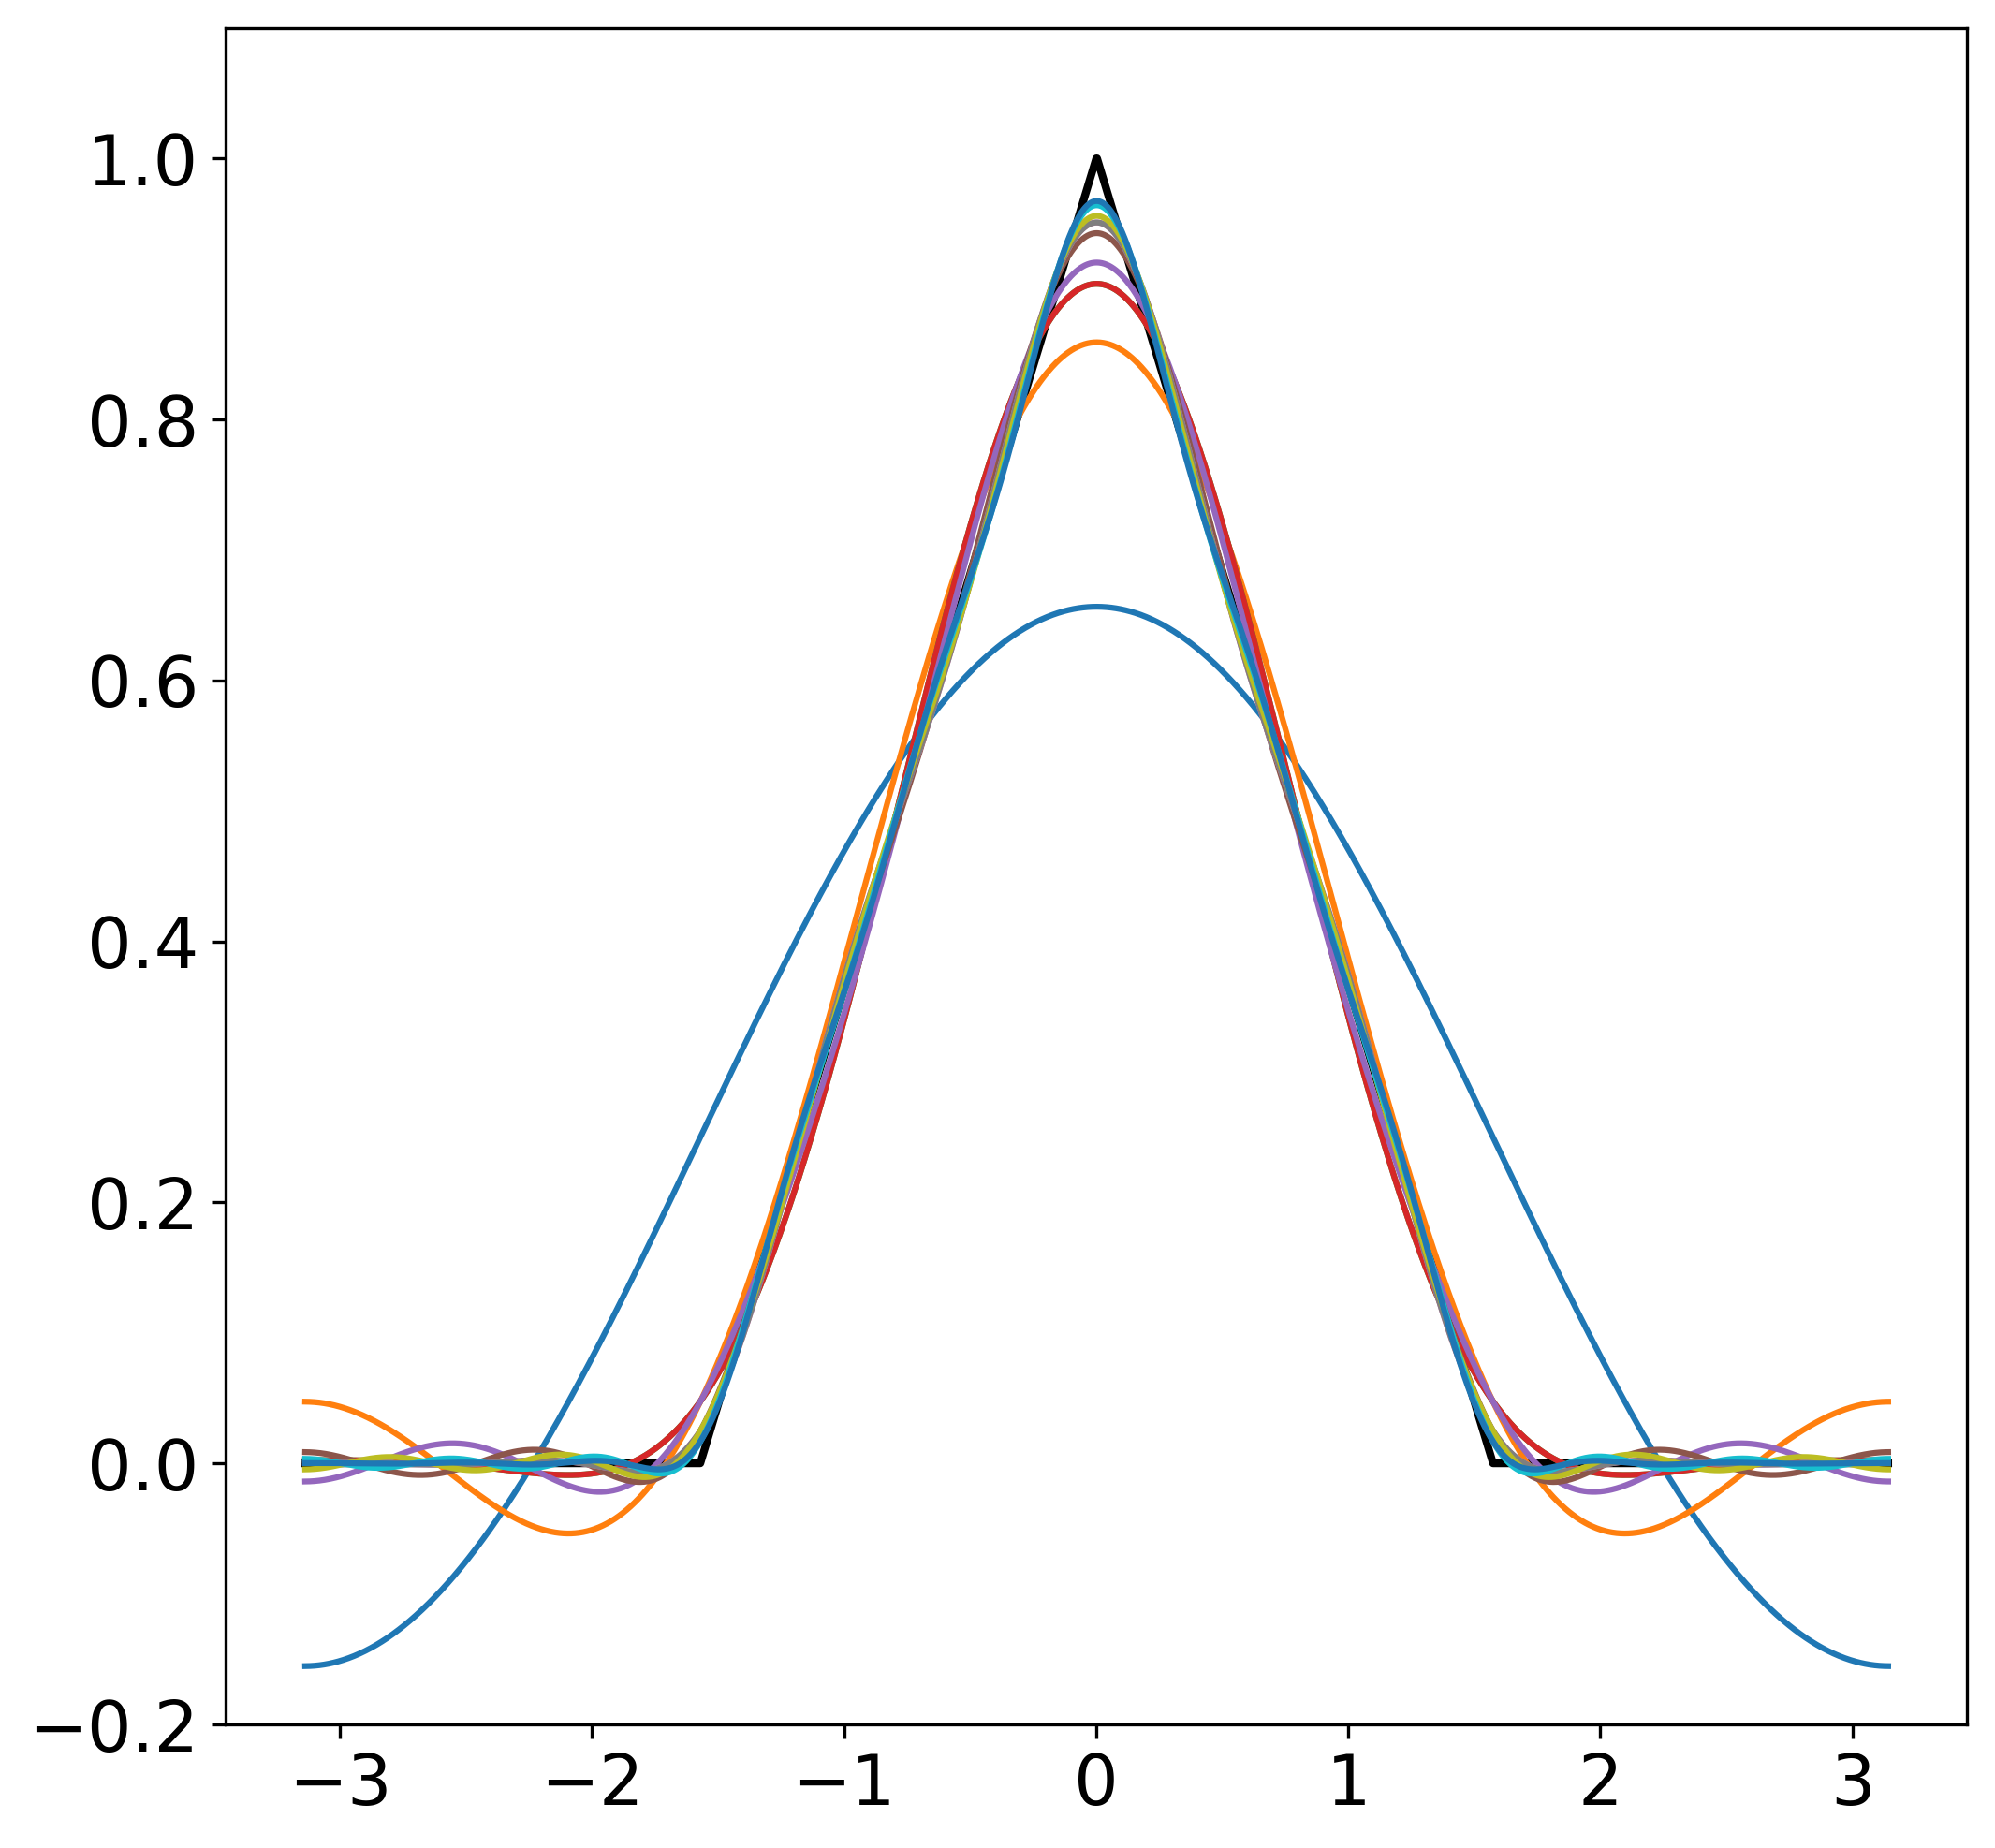
\includegraphics[width=.5\linewidth]{programs/fourier1/out_11.png}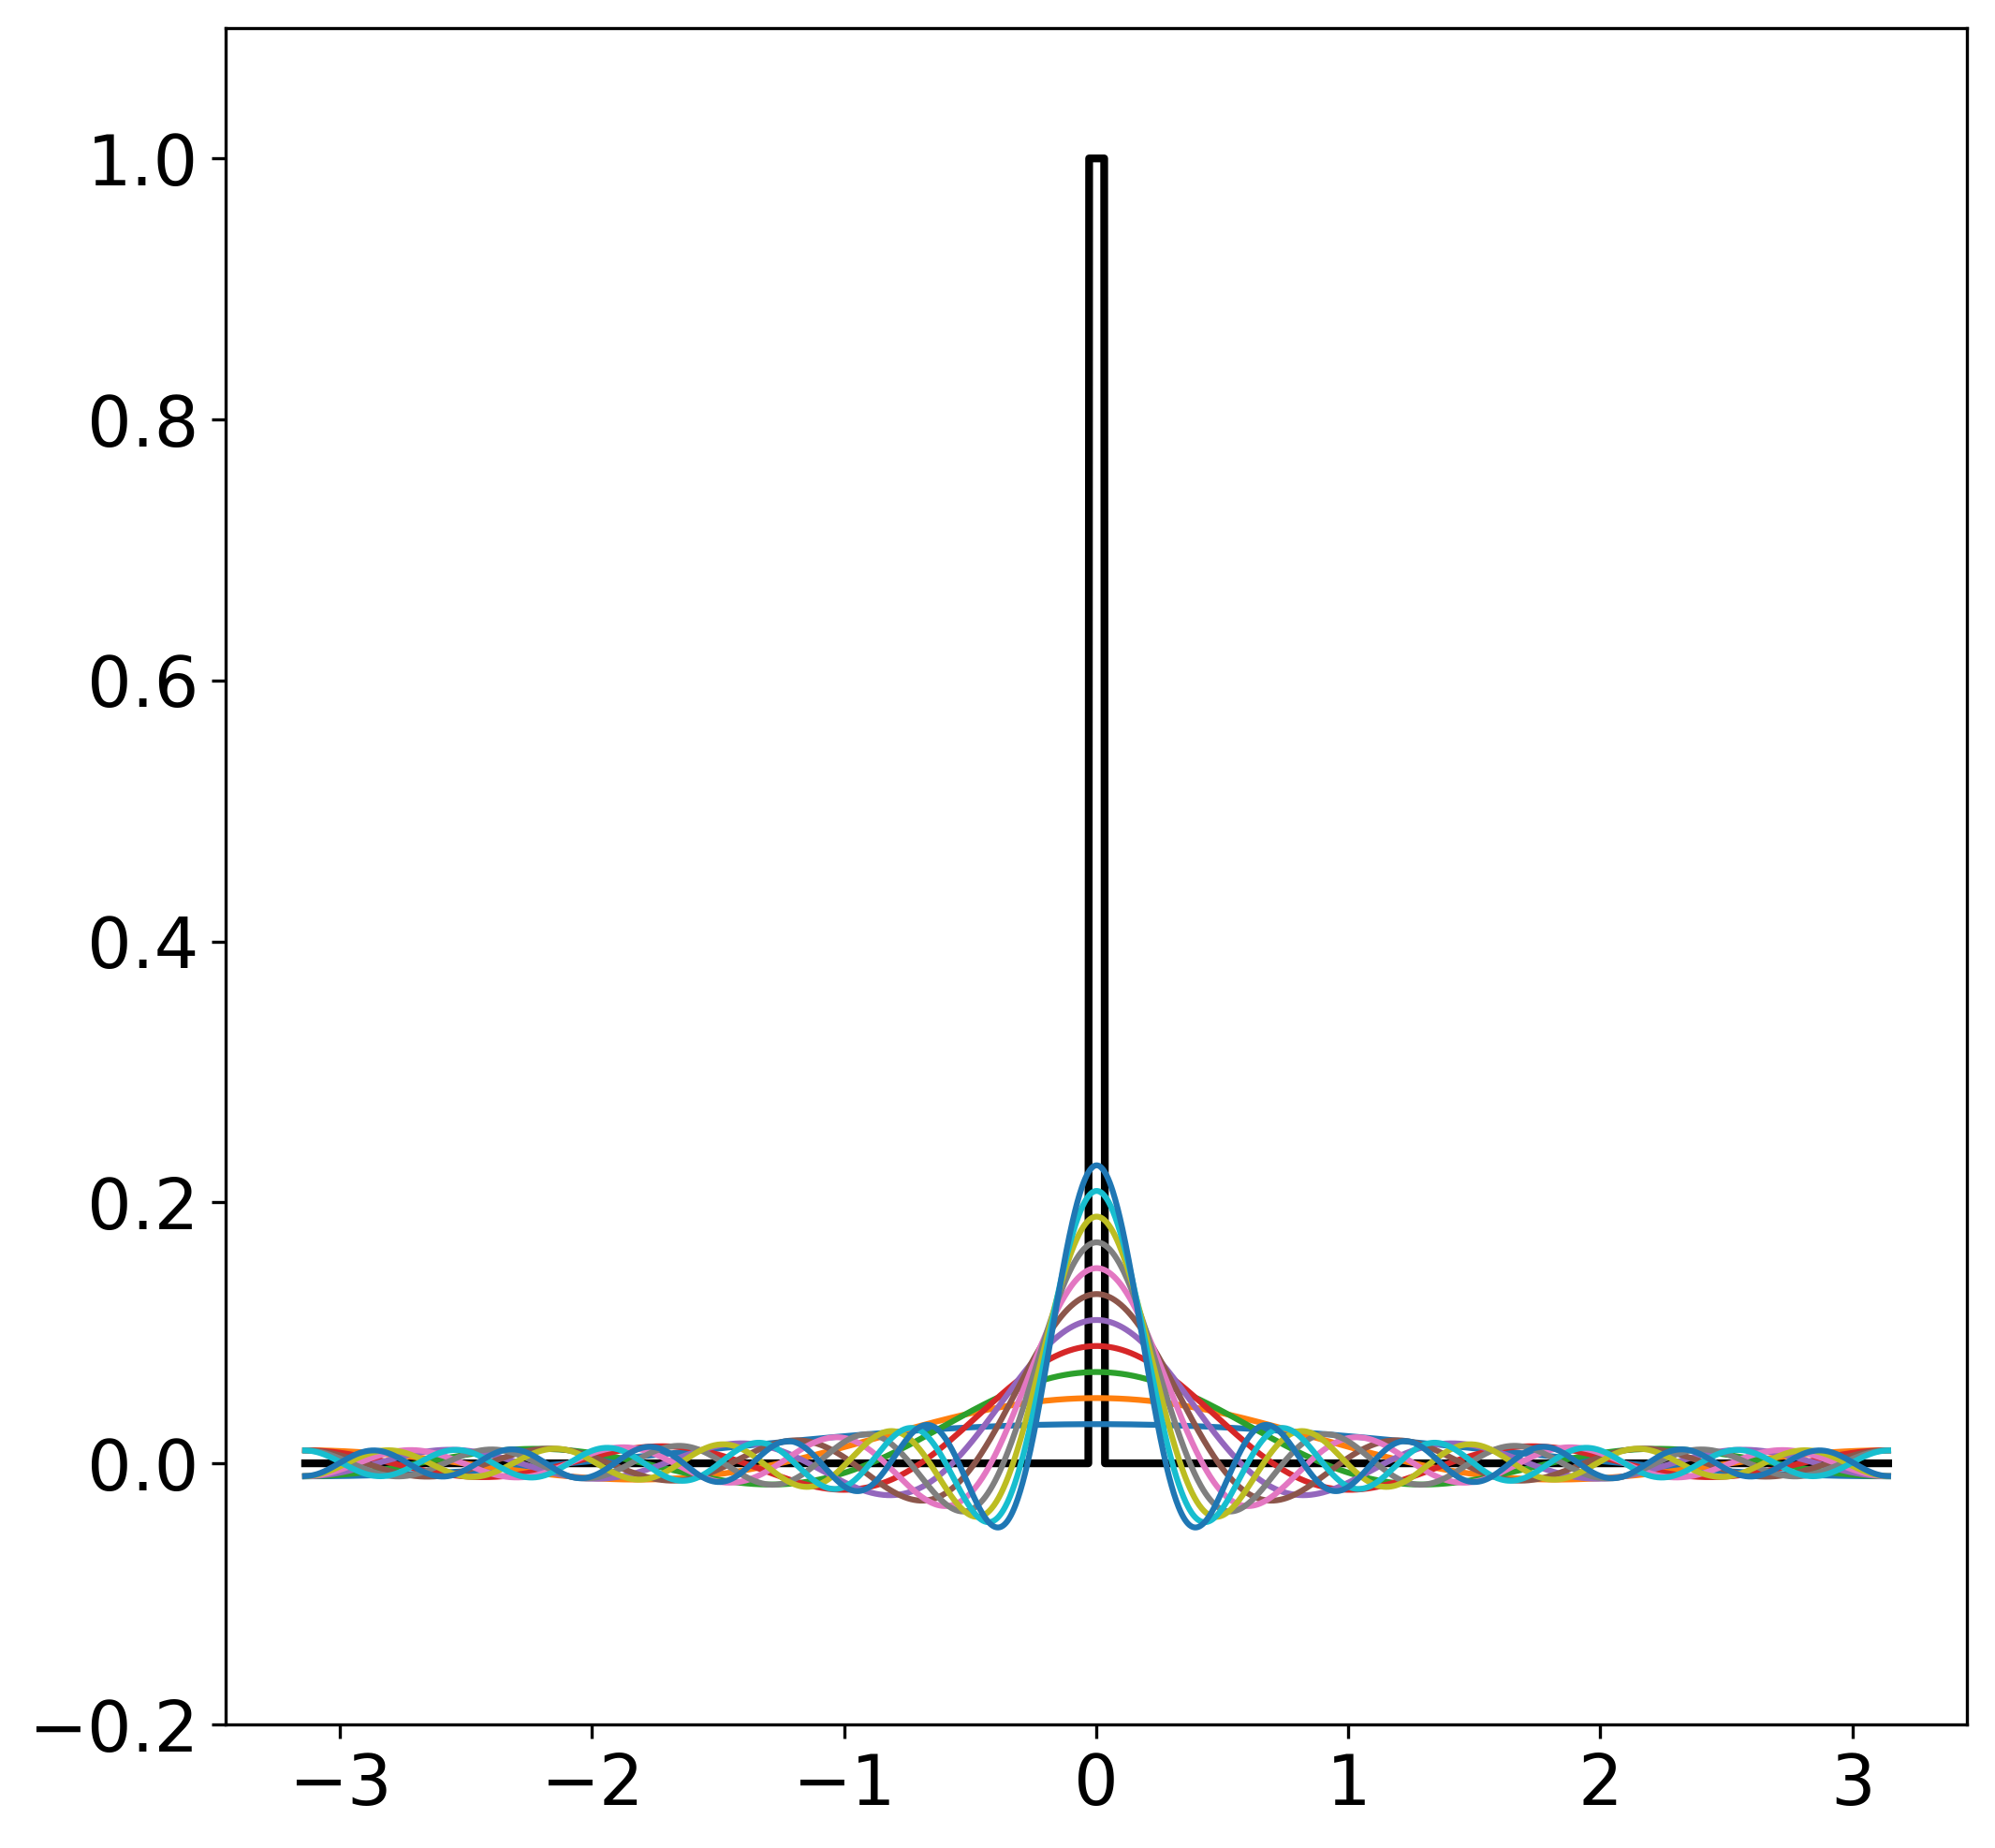
\includegraphics[width=.5\linewidth]{programs/fourier2/out_11.png}}
    \only<13|handout:0>{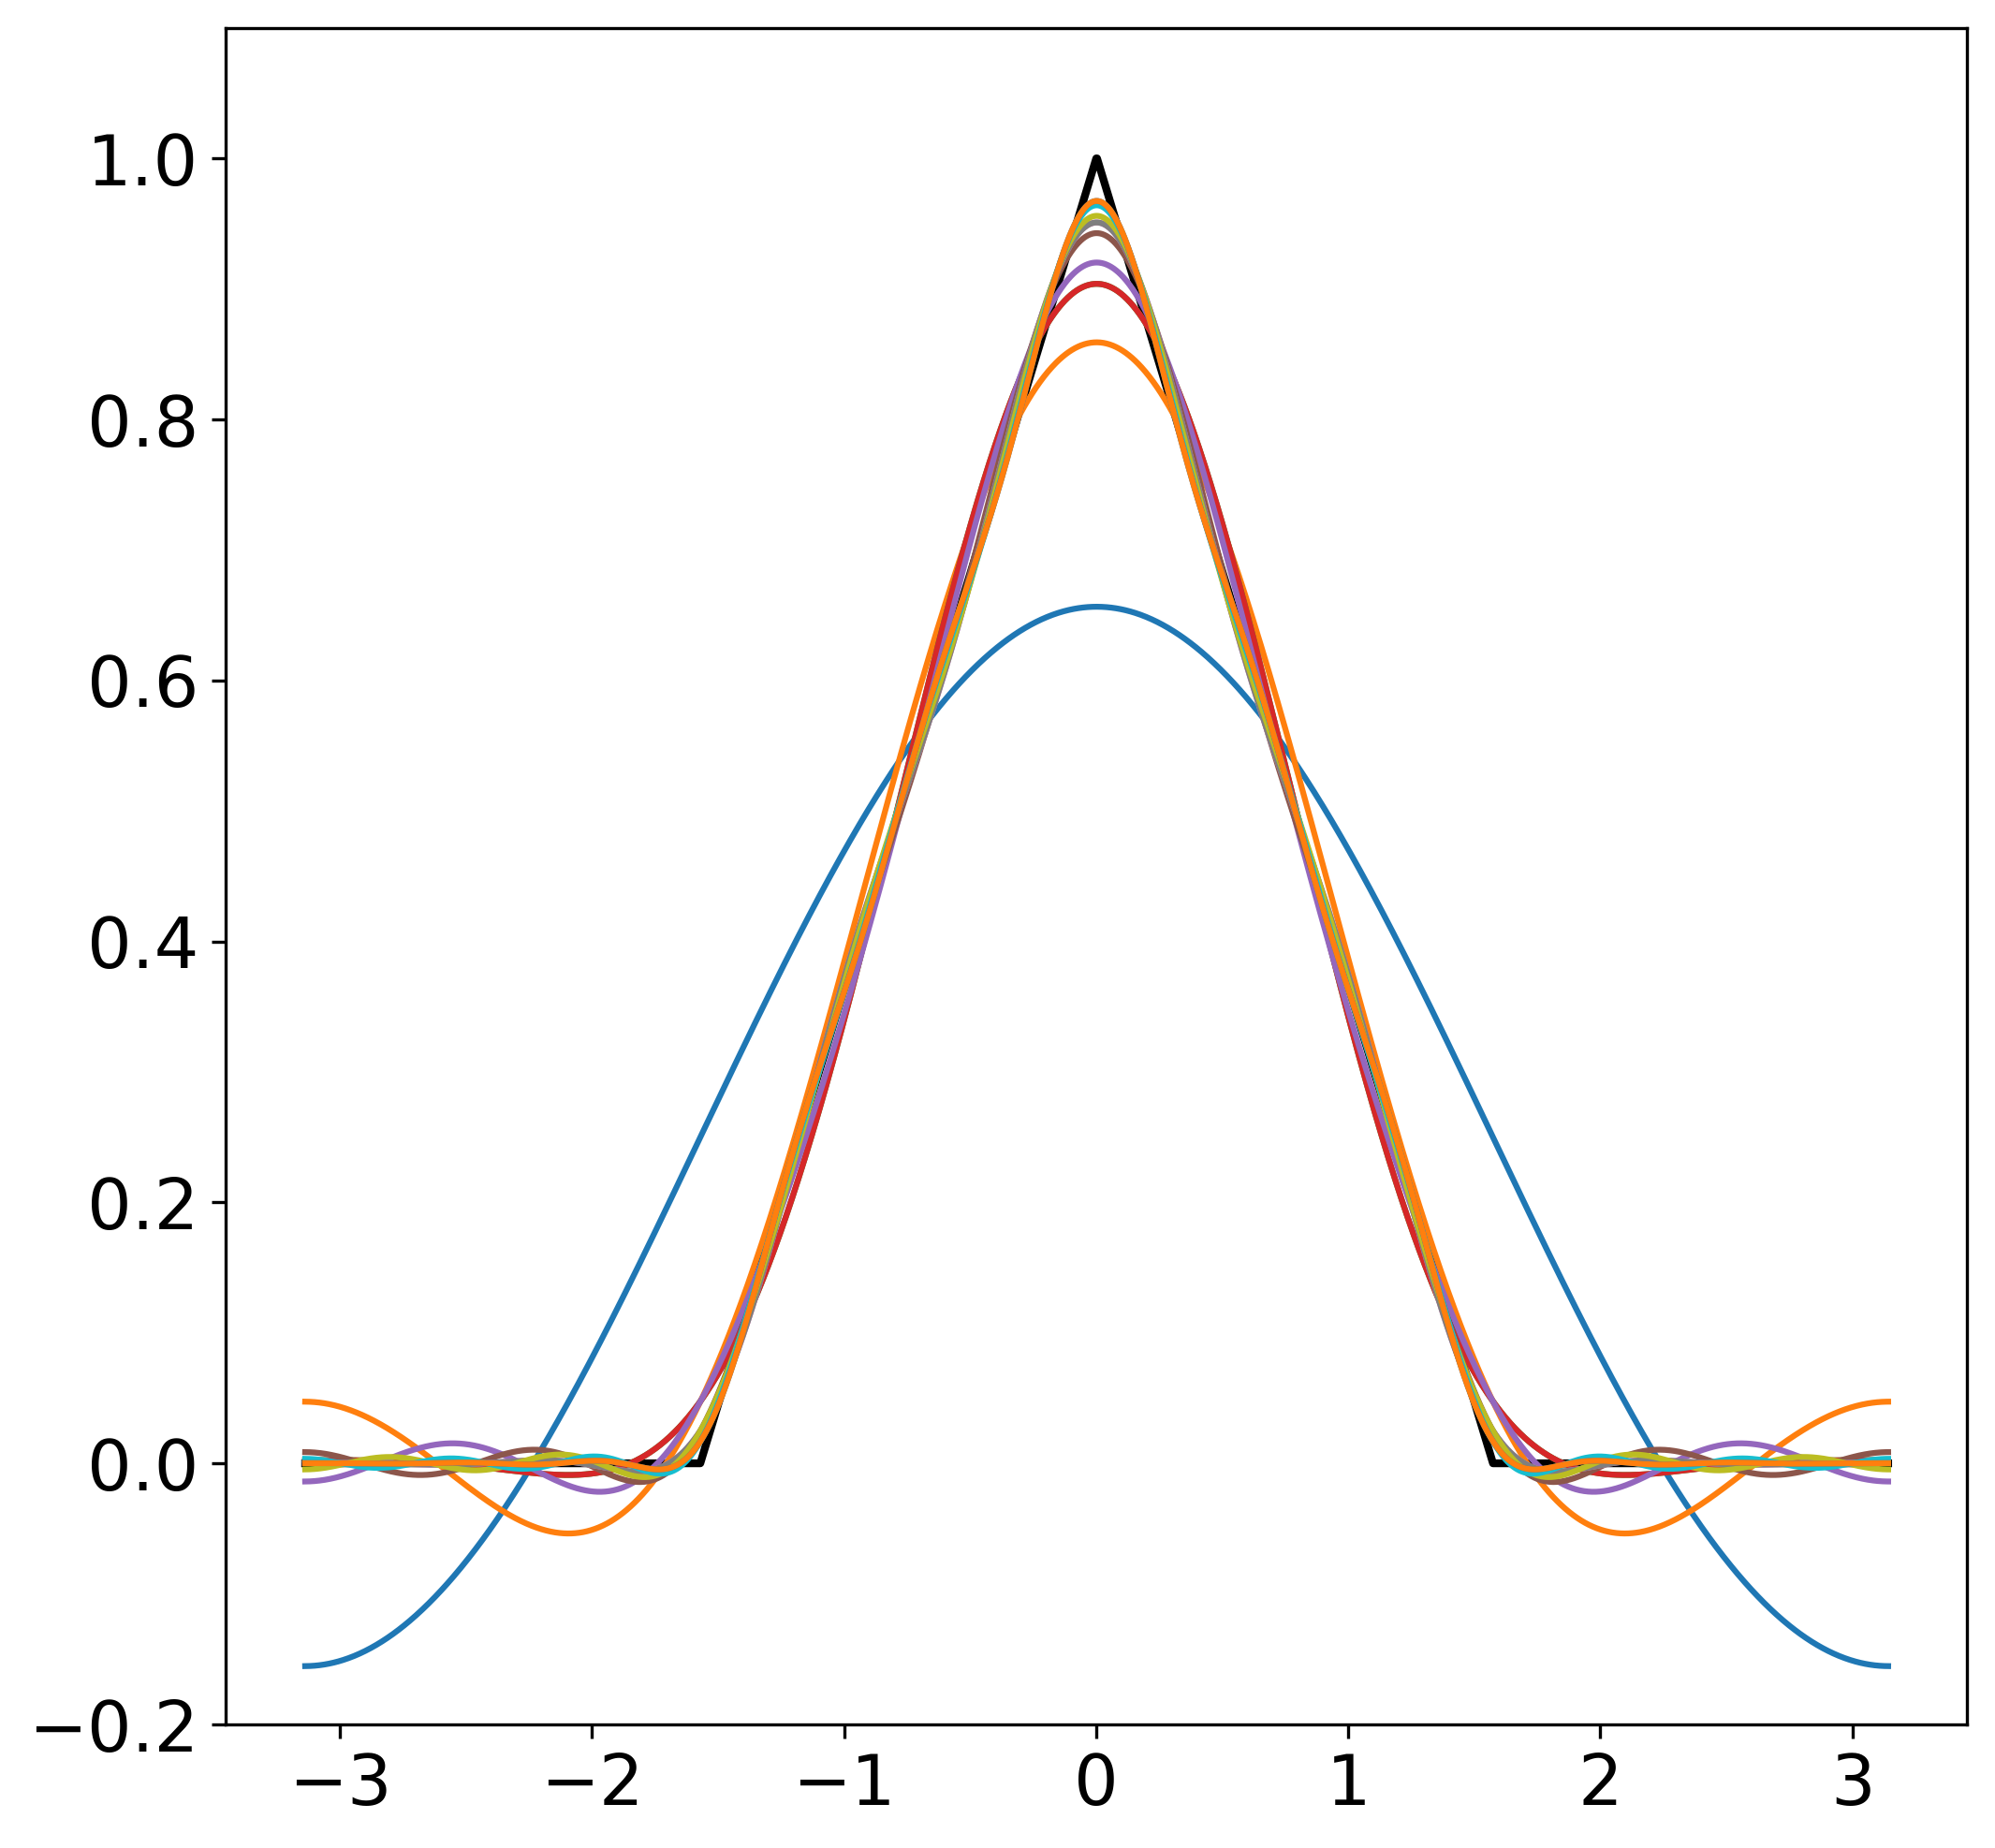
\includegraphics[width=.5\linewidth]{programs/fourier1/out_12.png}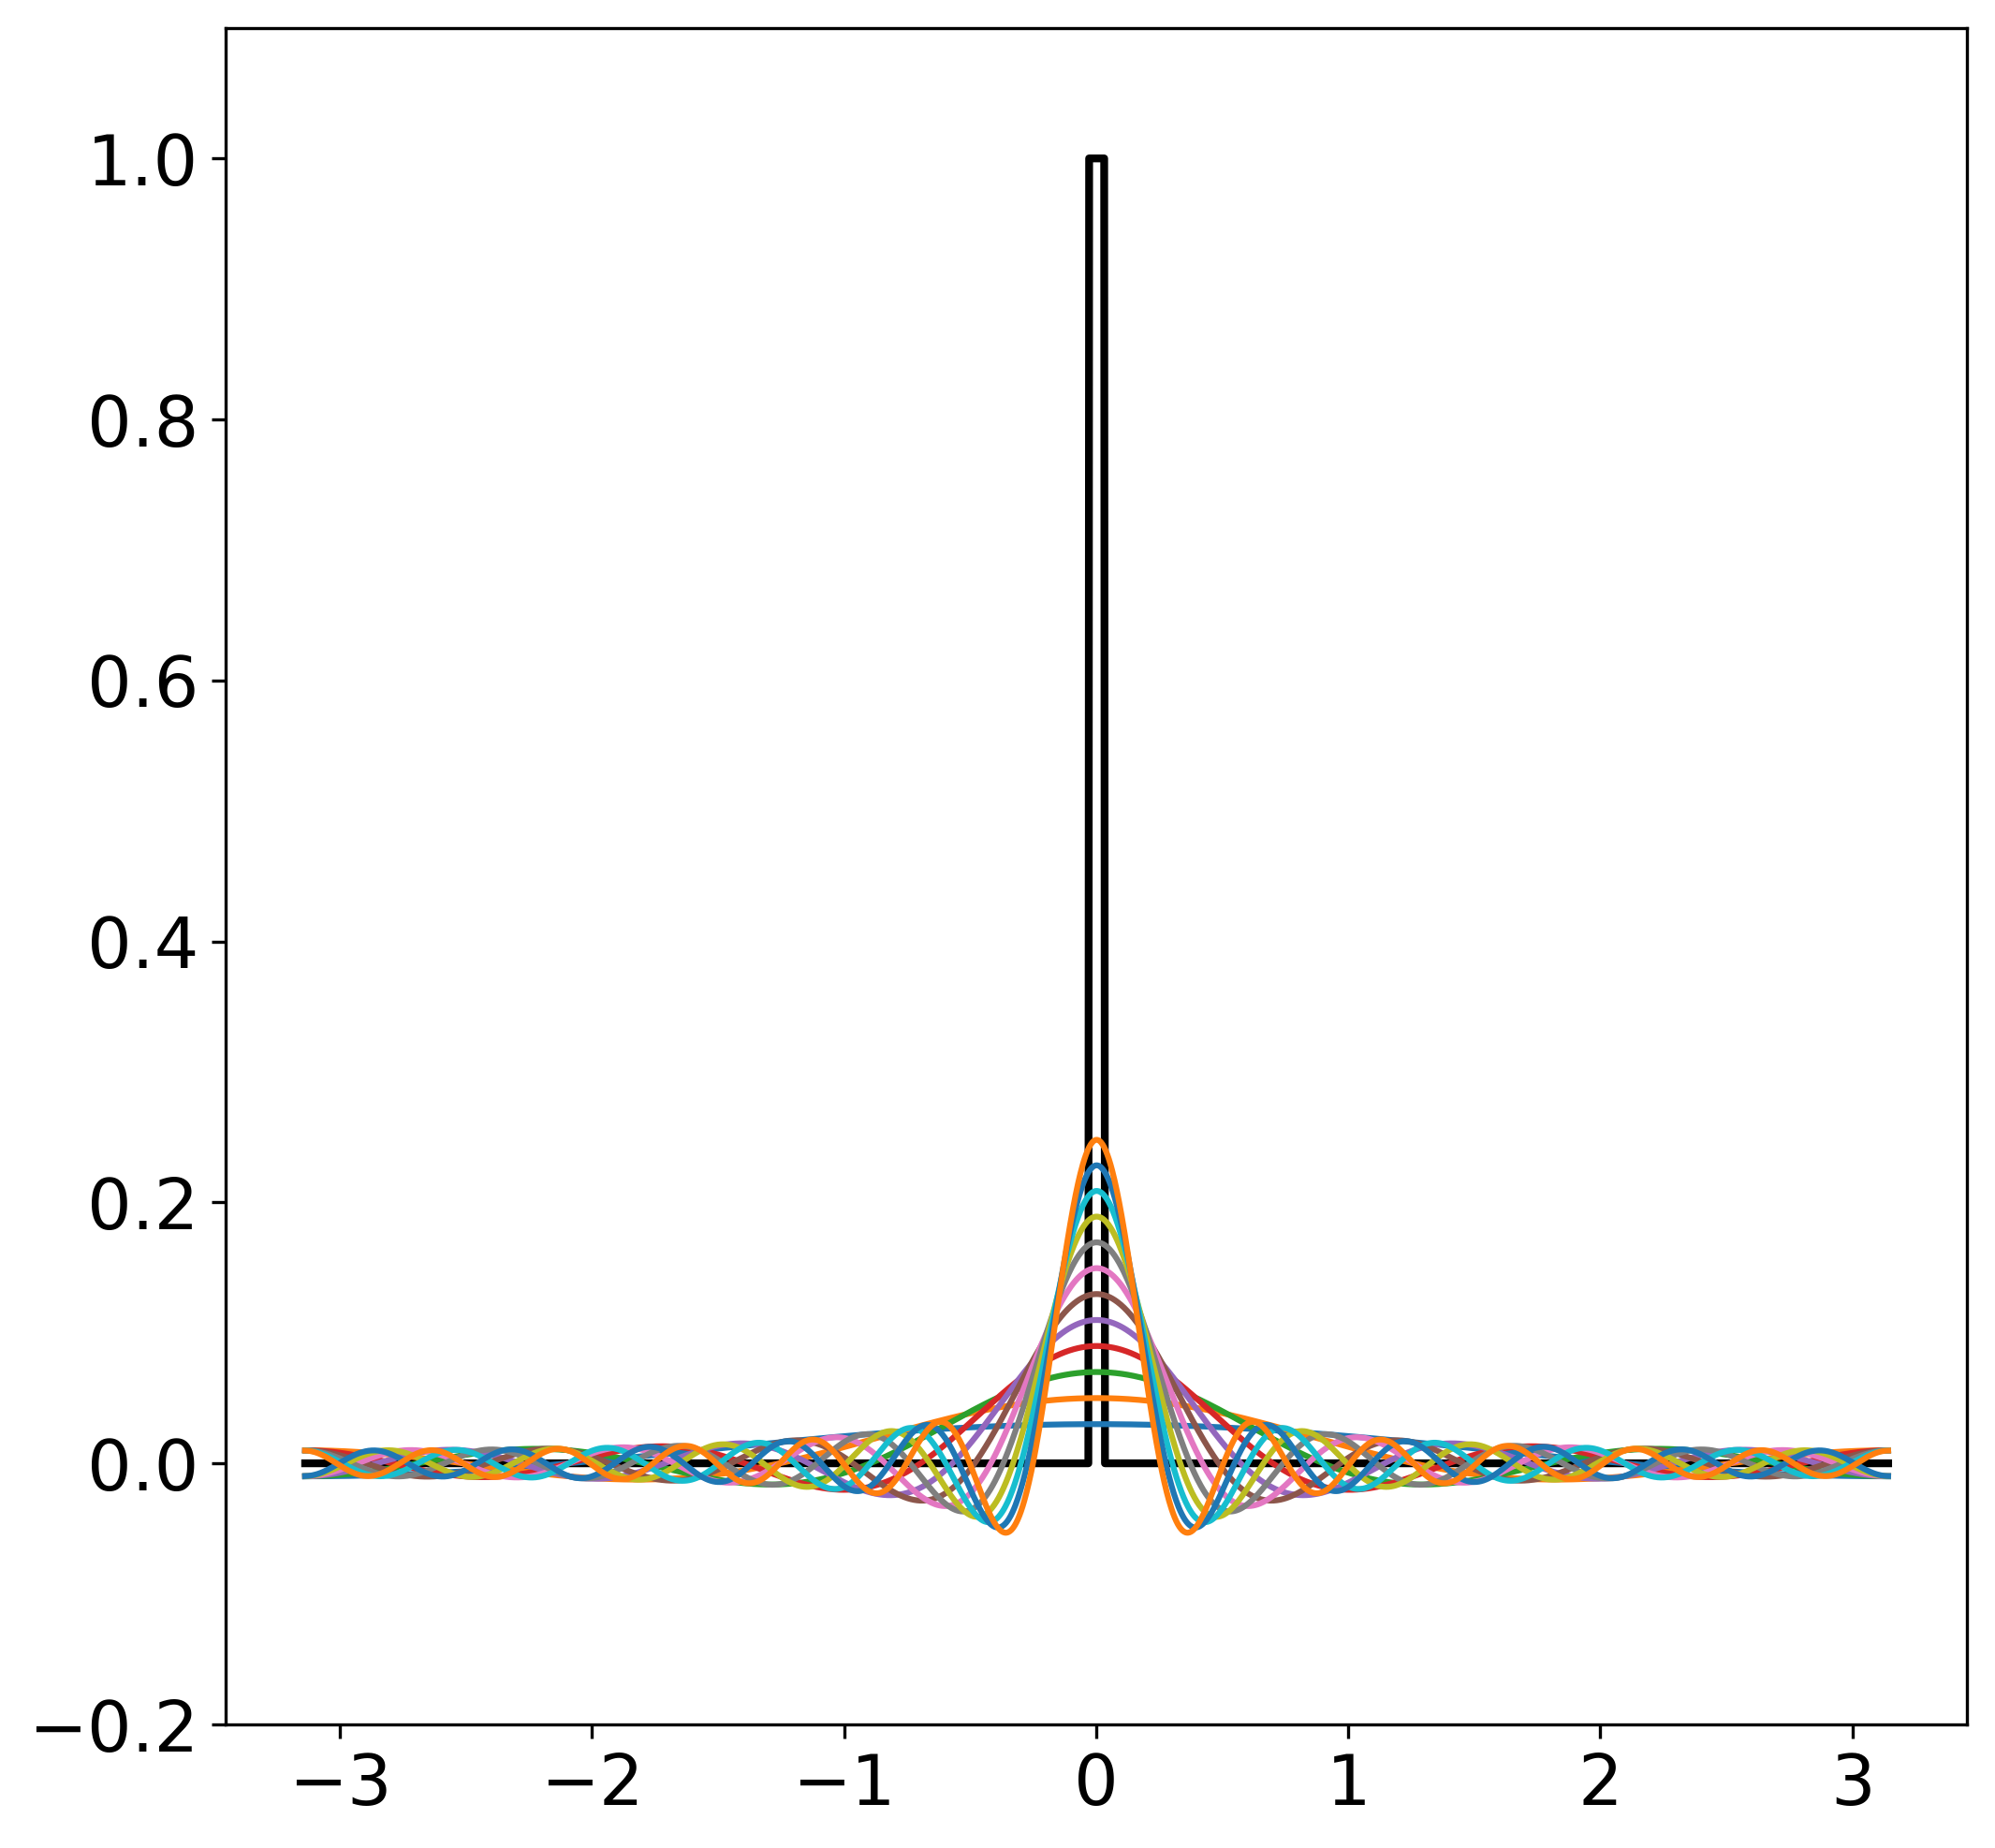
\includegraphics[width=.5\linewidth]{programs/fourier2/out_12.png}}
    \only<14|handout:0>{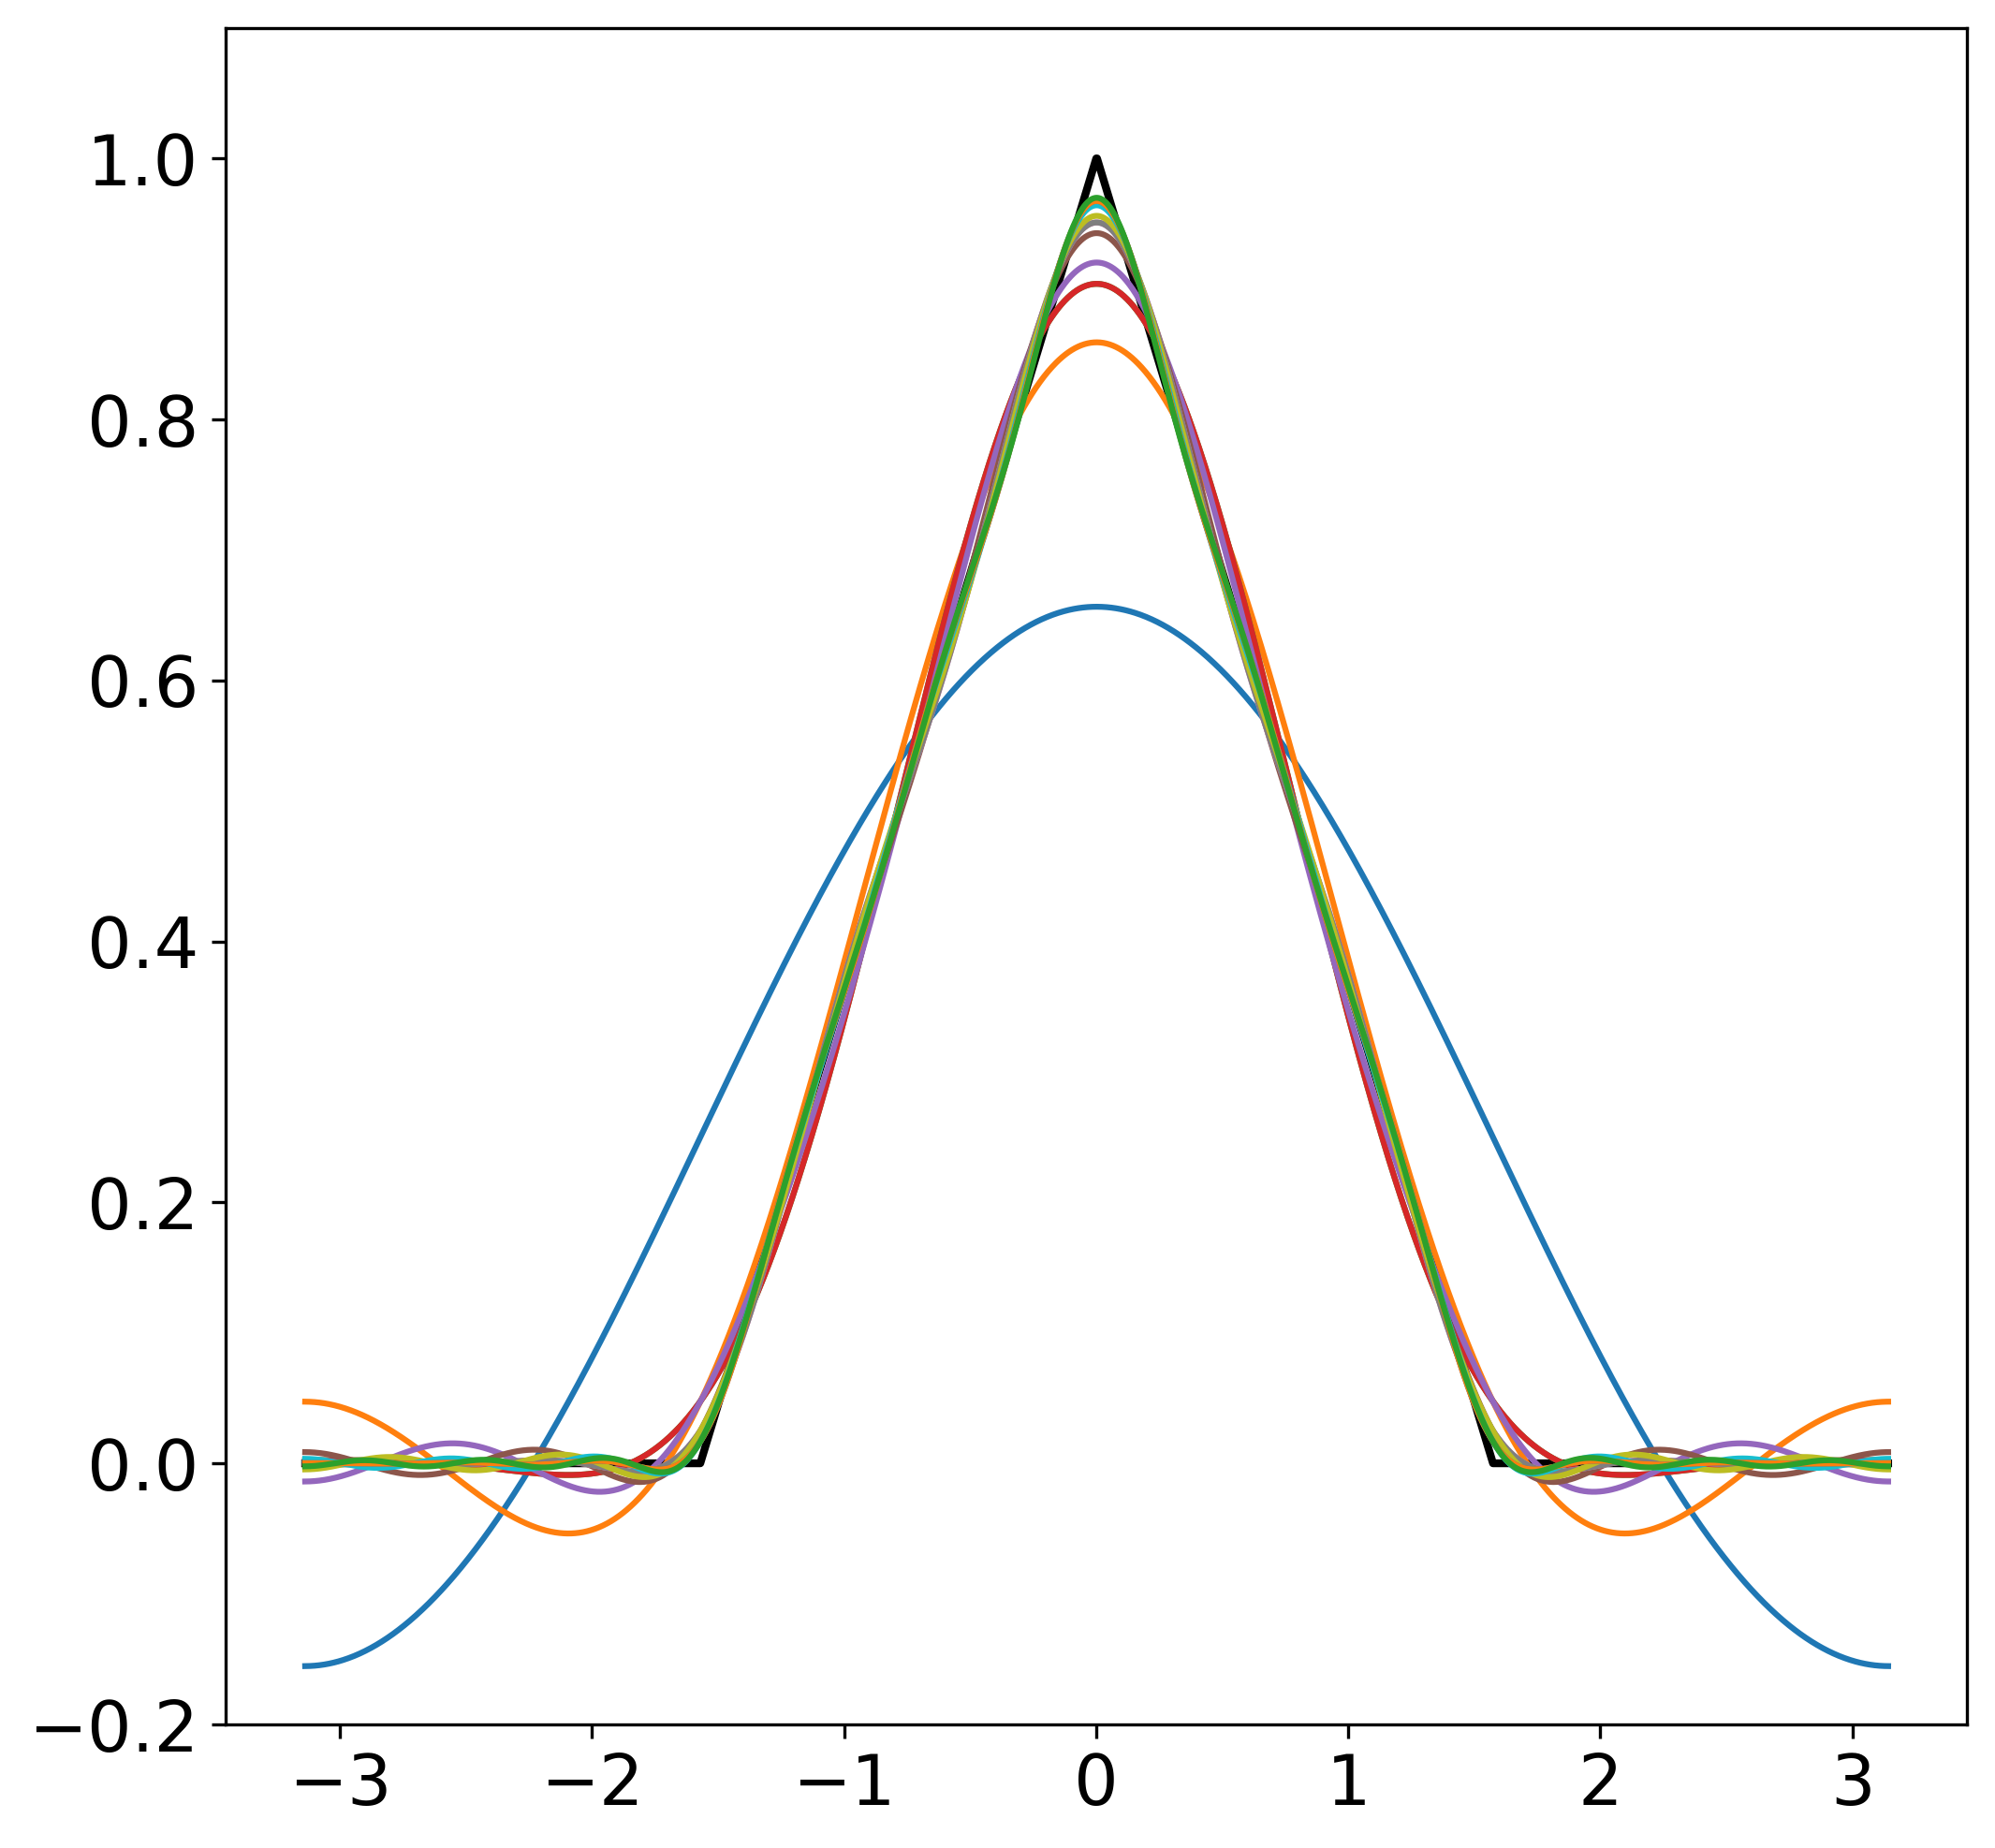
\includegraphics[width=.5\linewidth]{programs/fourier1/out_13.png}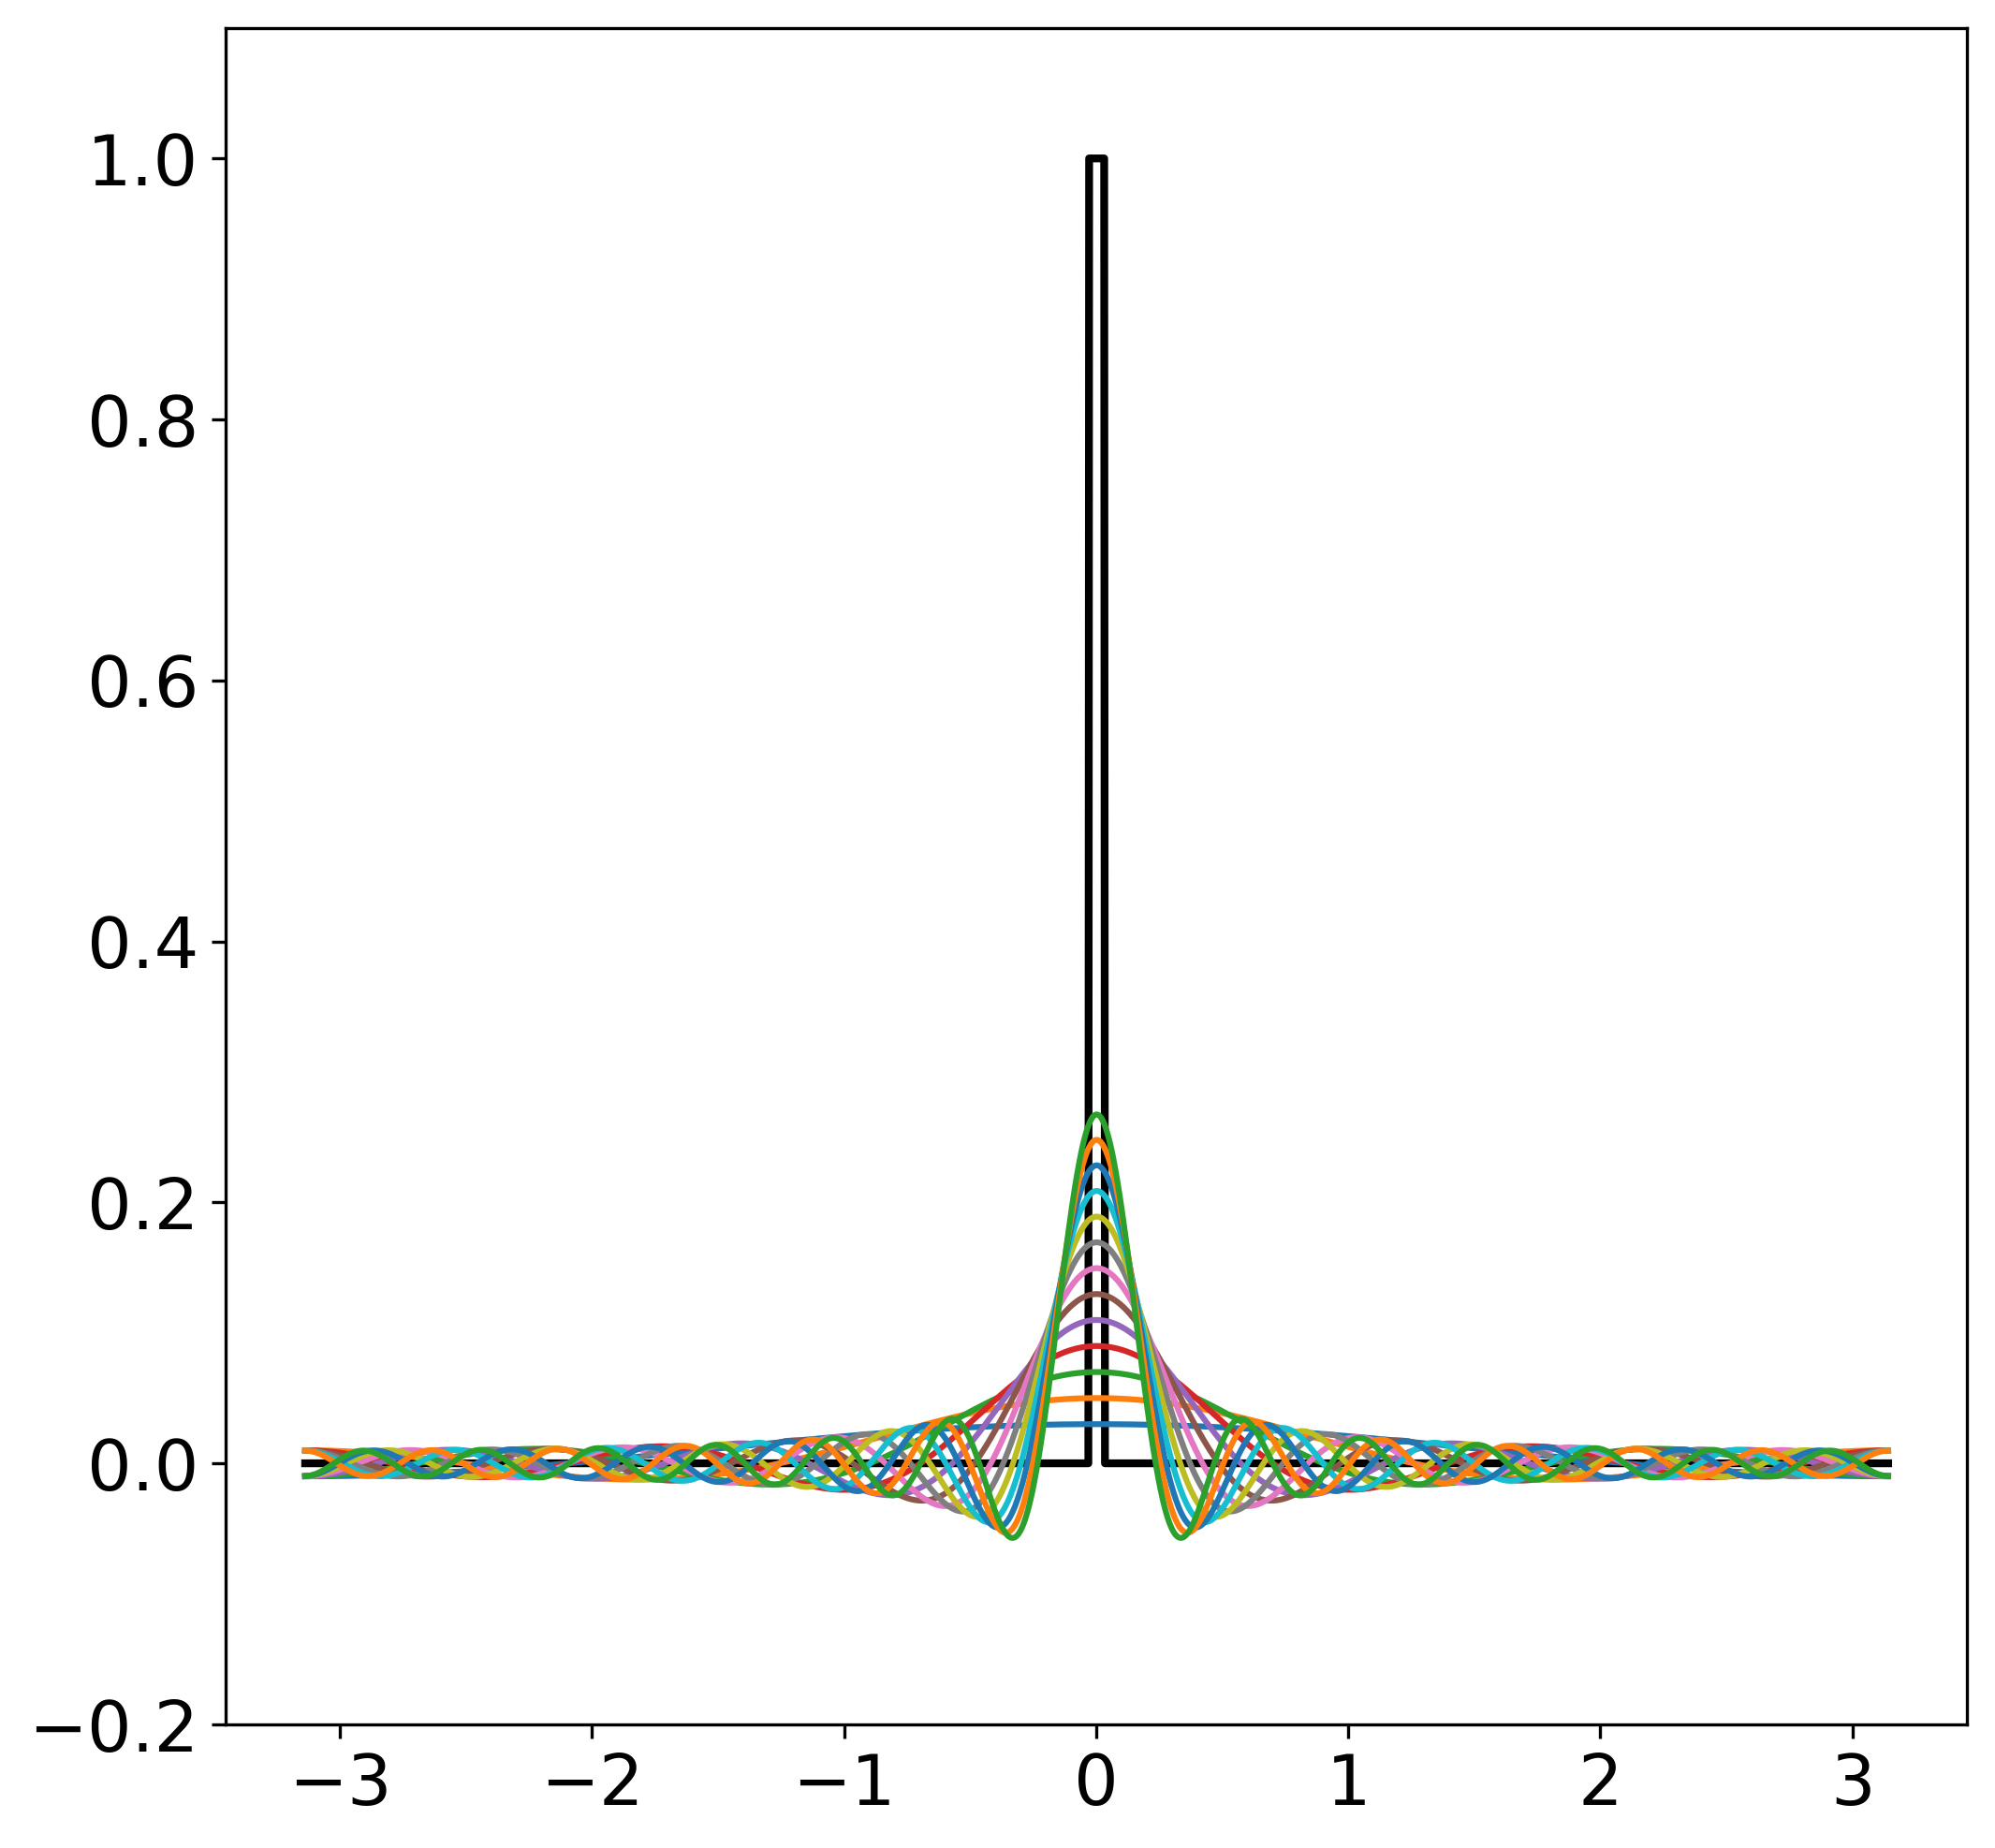
\includegraphics[width=.5\linewidth]{programs/fourier2/out_13.png}}
    \only<15|handout:0>{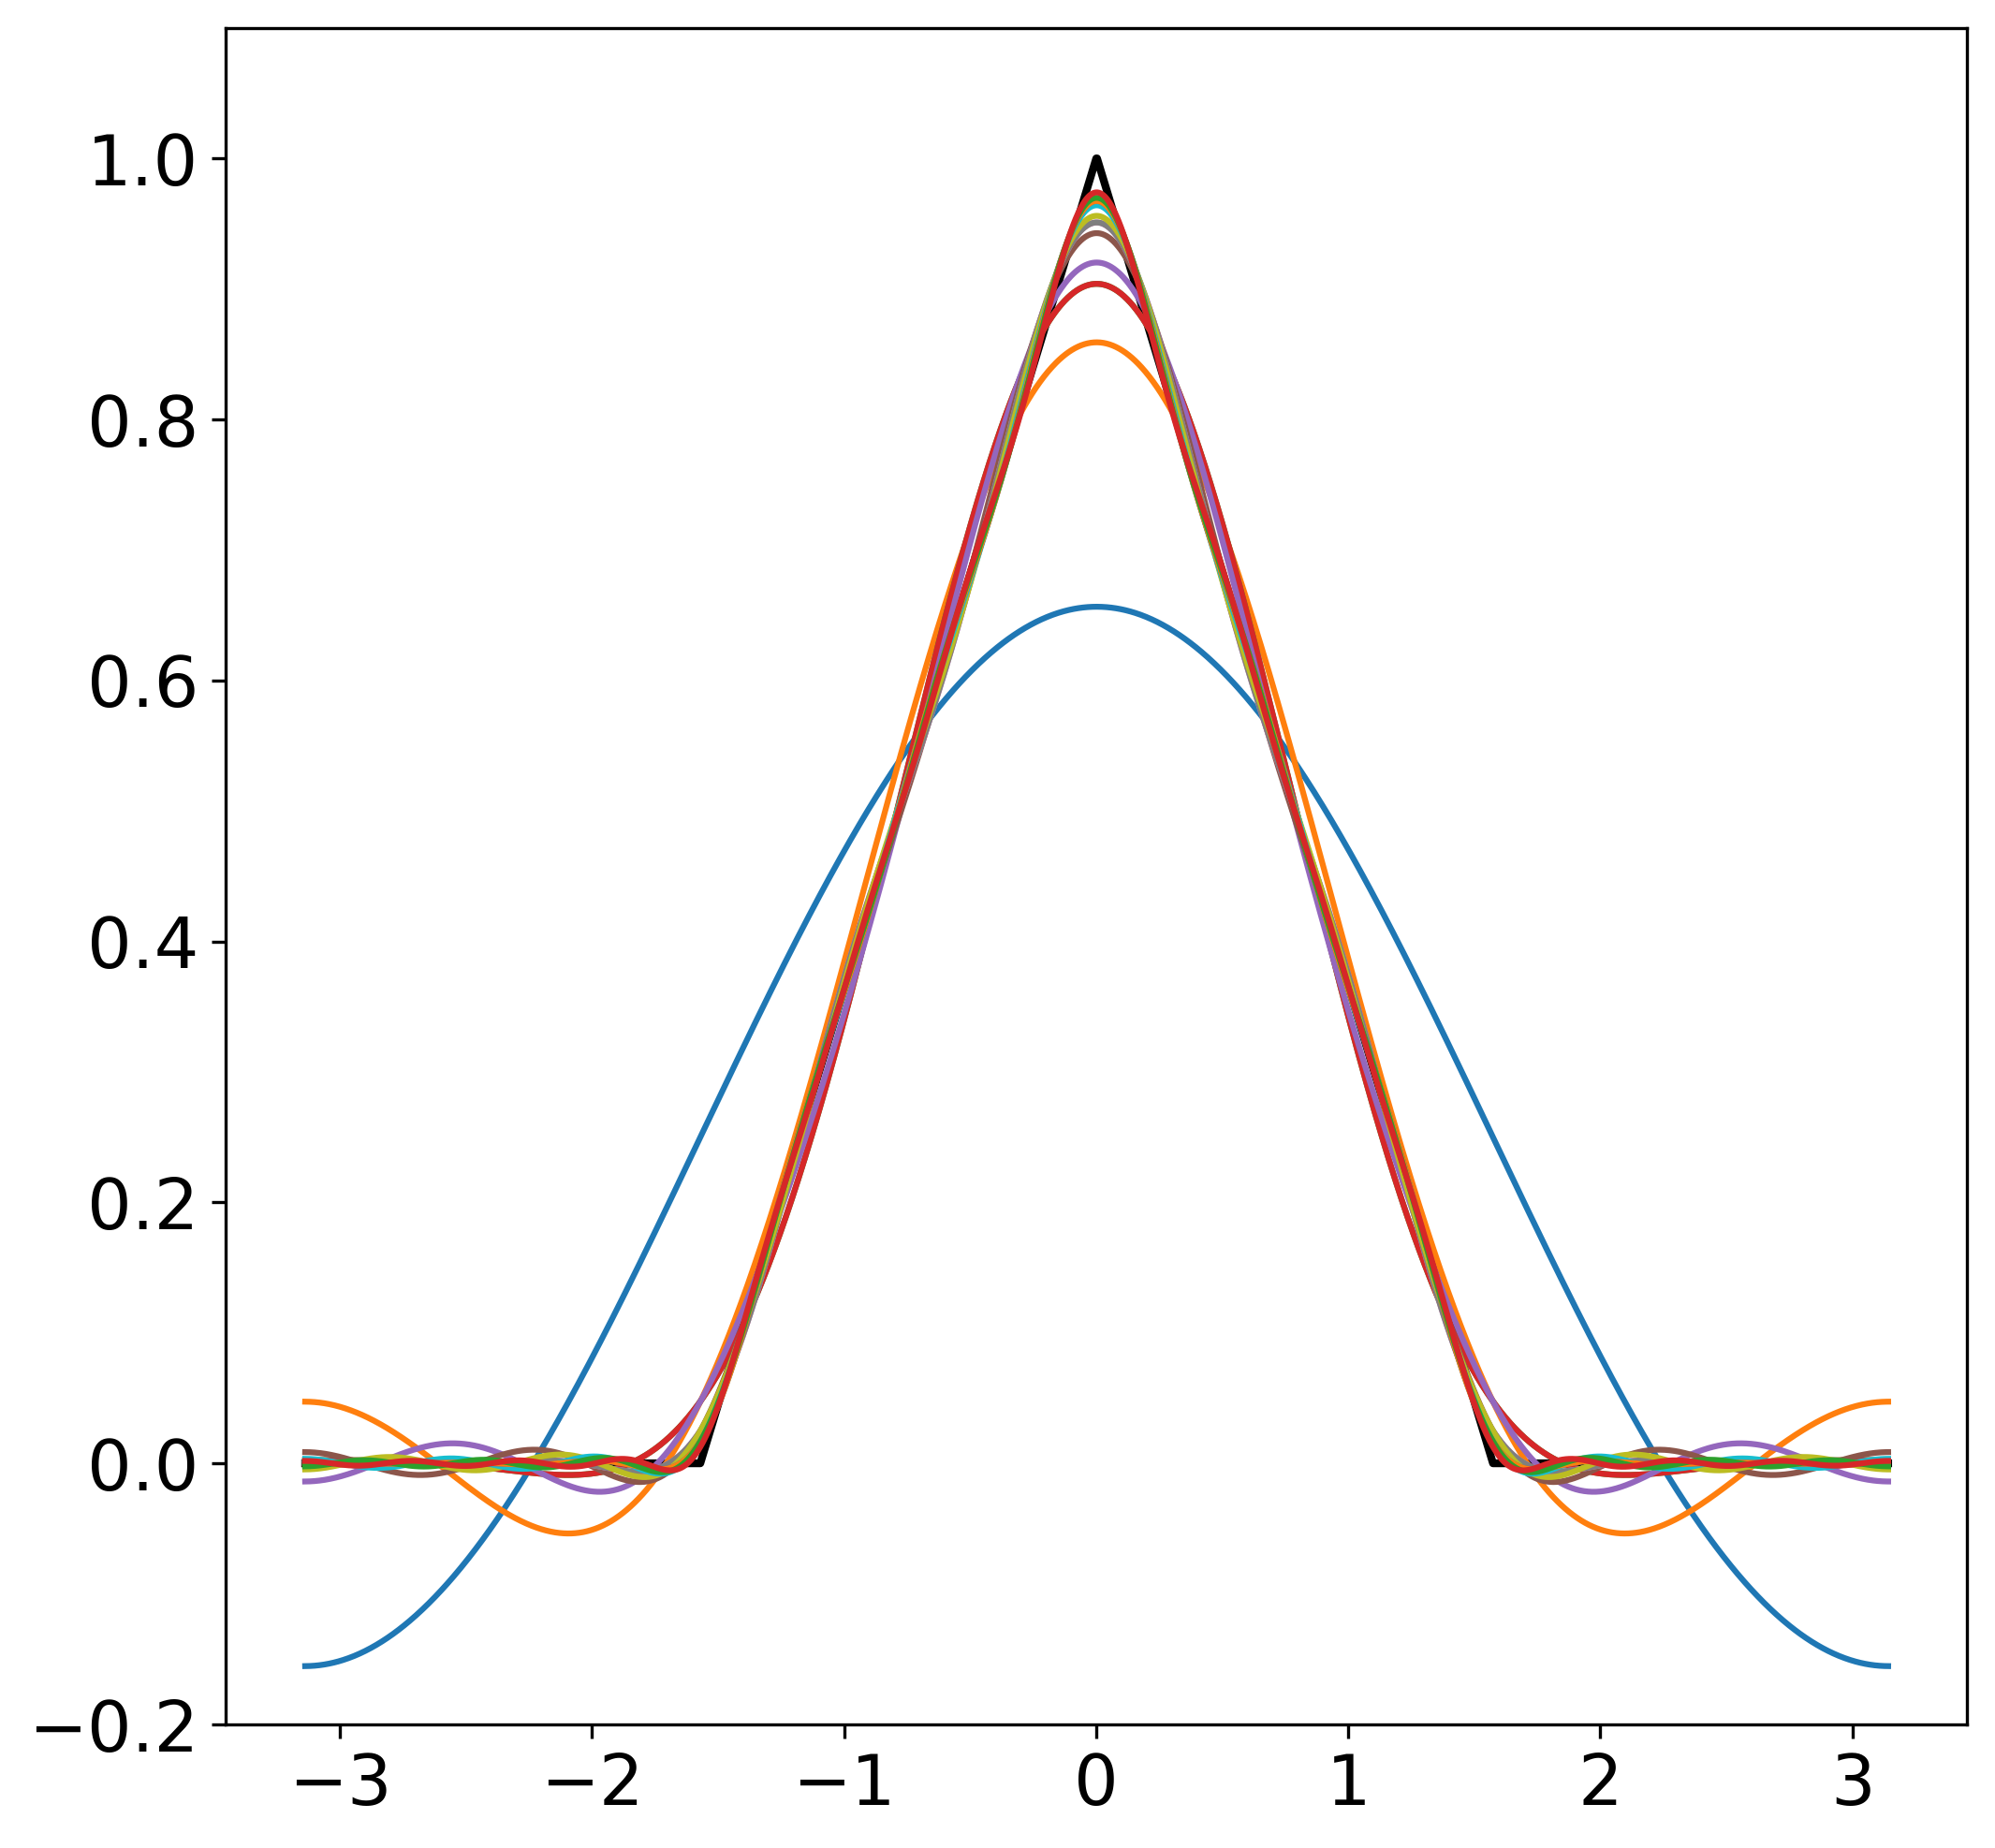
\includegraphics[width=.5\linewidth]{programs/fourier1/out_14.png}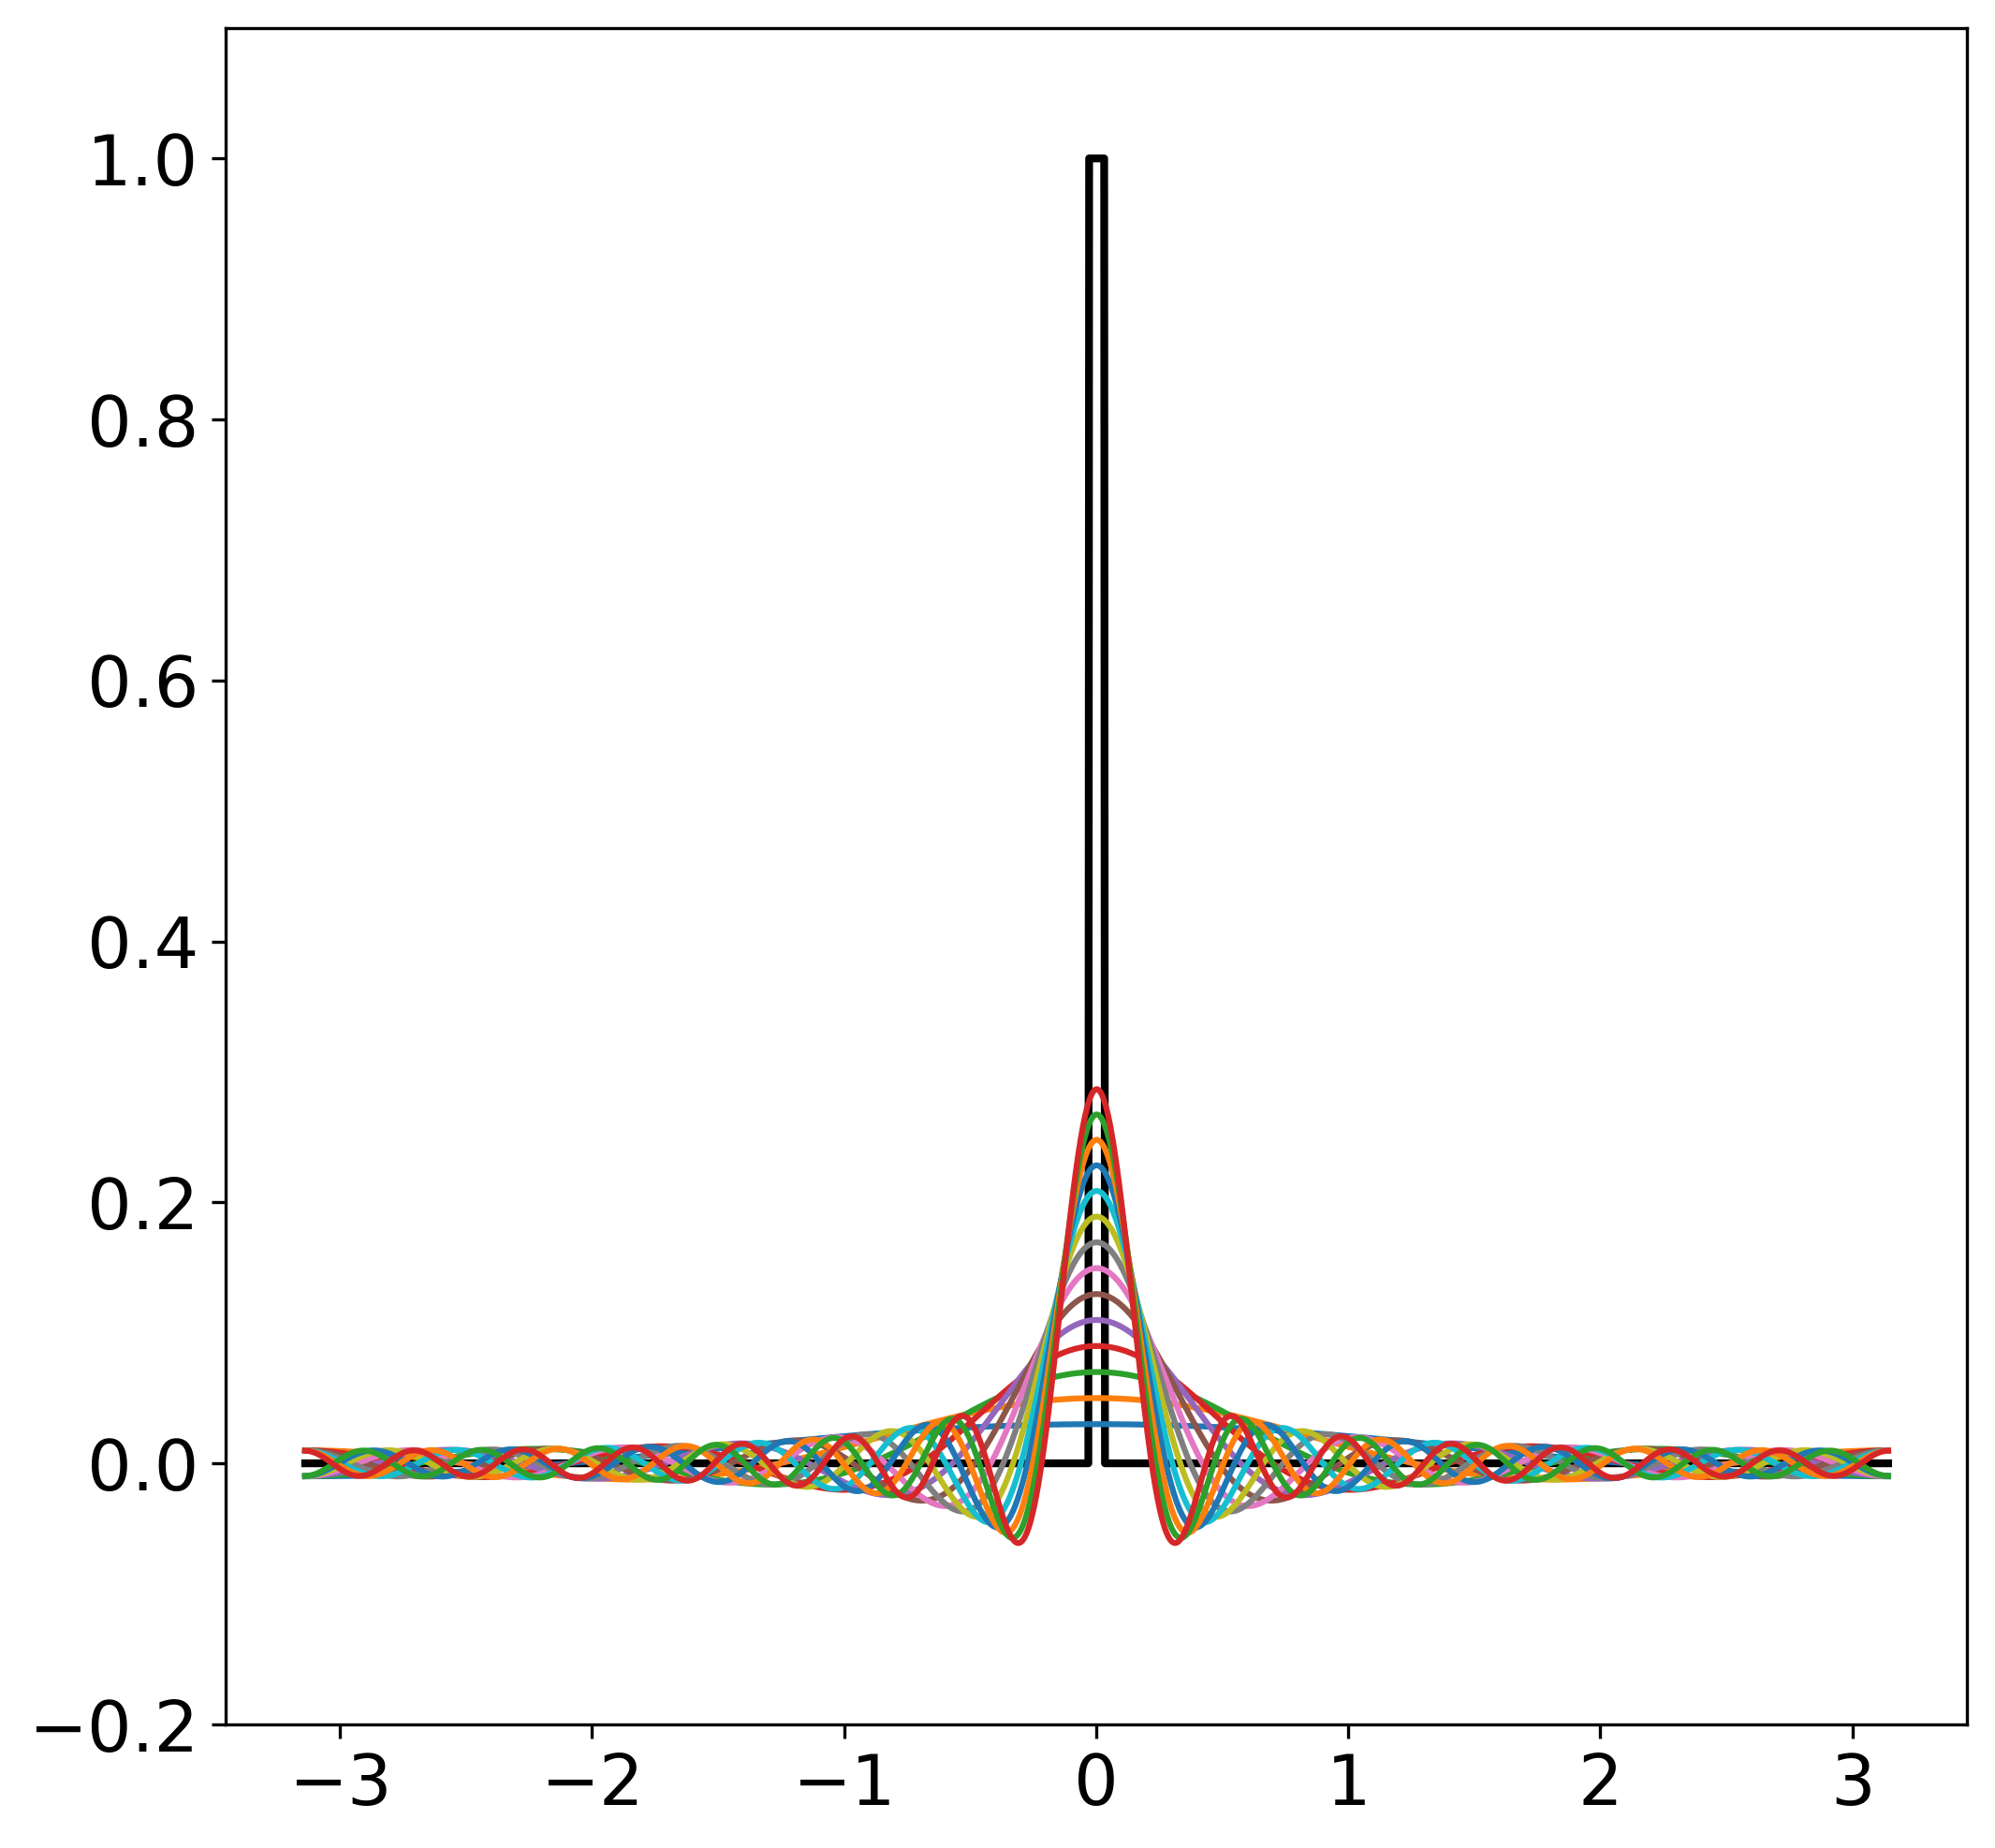
\includegraphics[width=.5\linewidth]{programs/fourier2/out_14.png}}
    \only<16|handout:0>{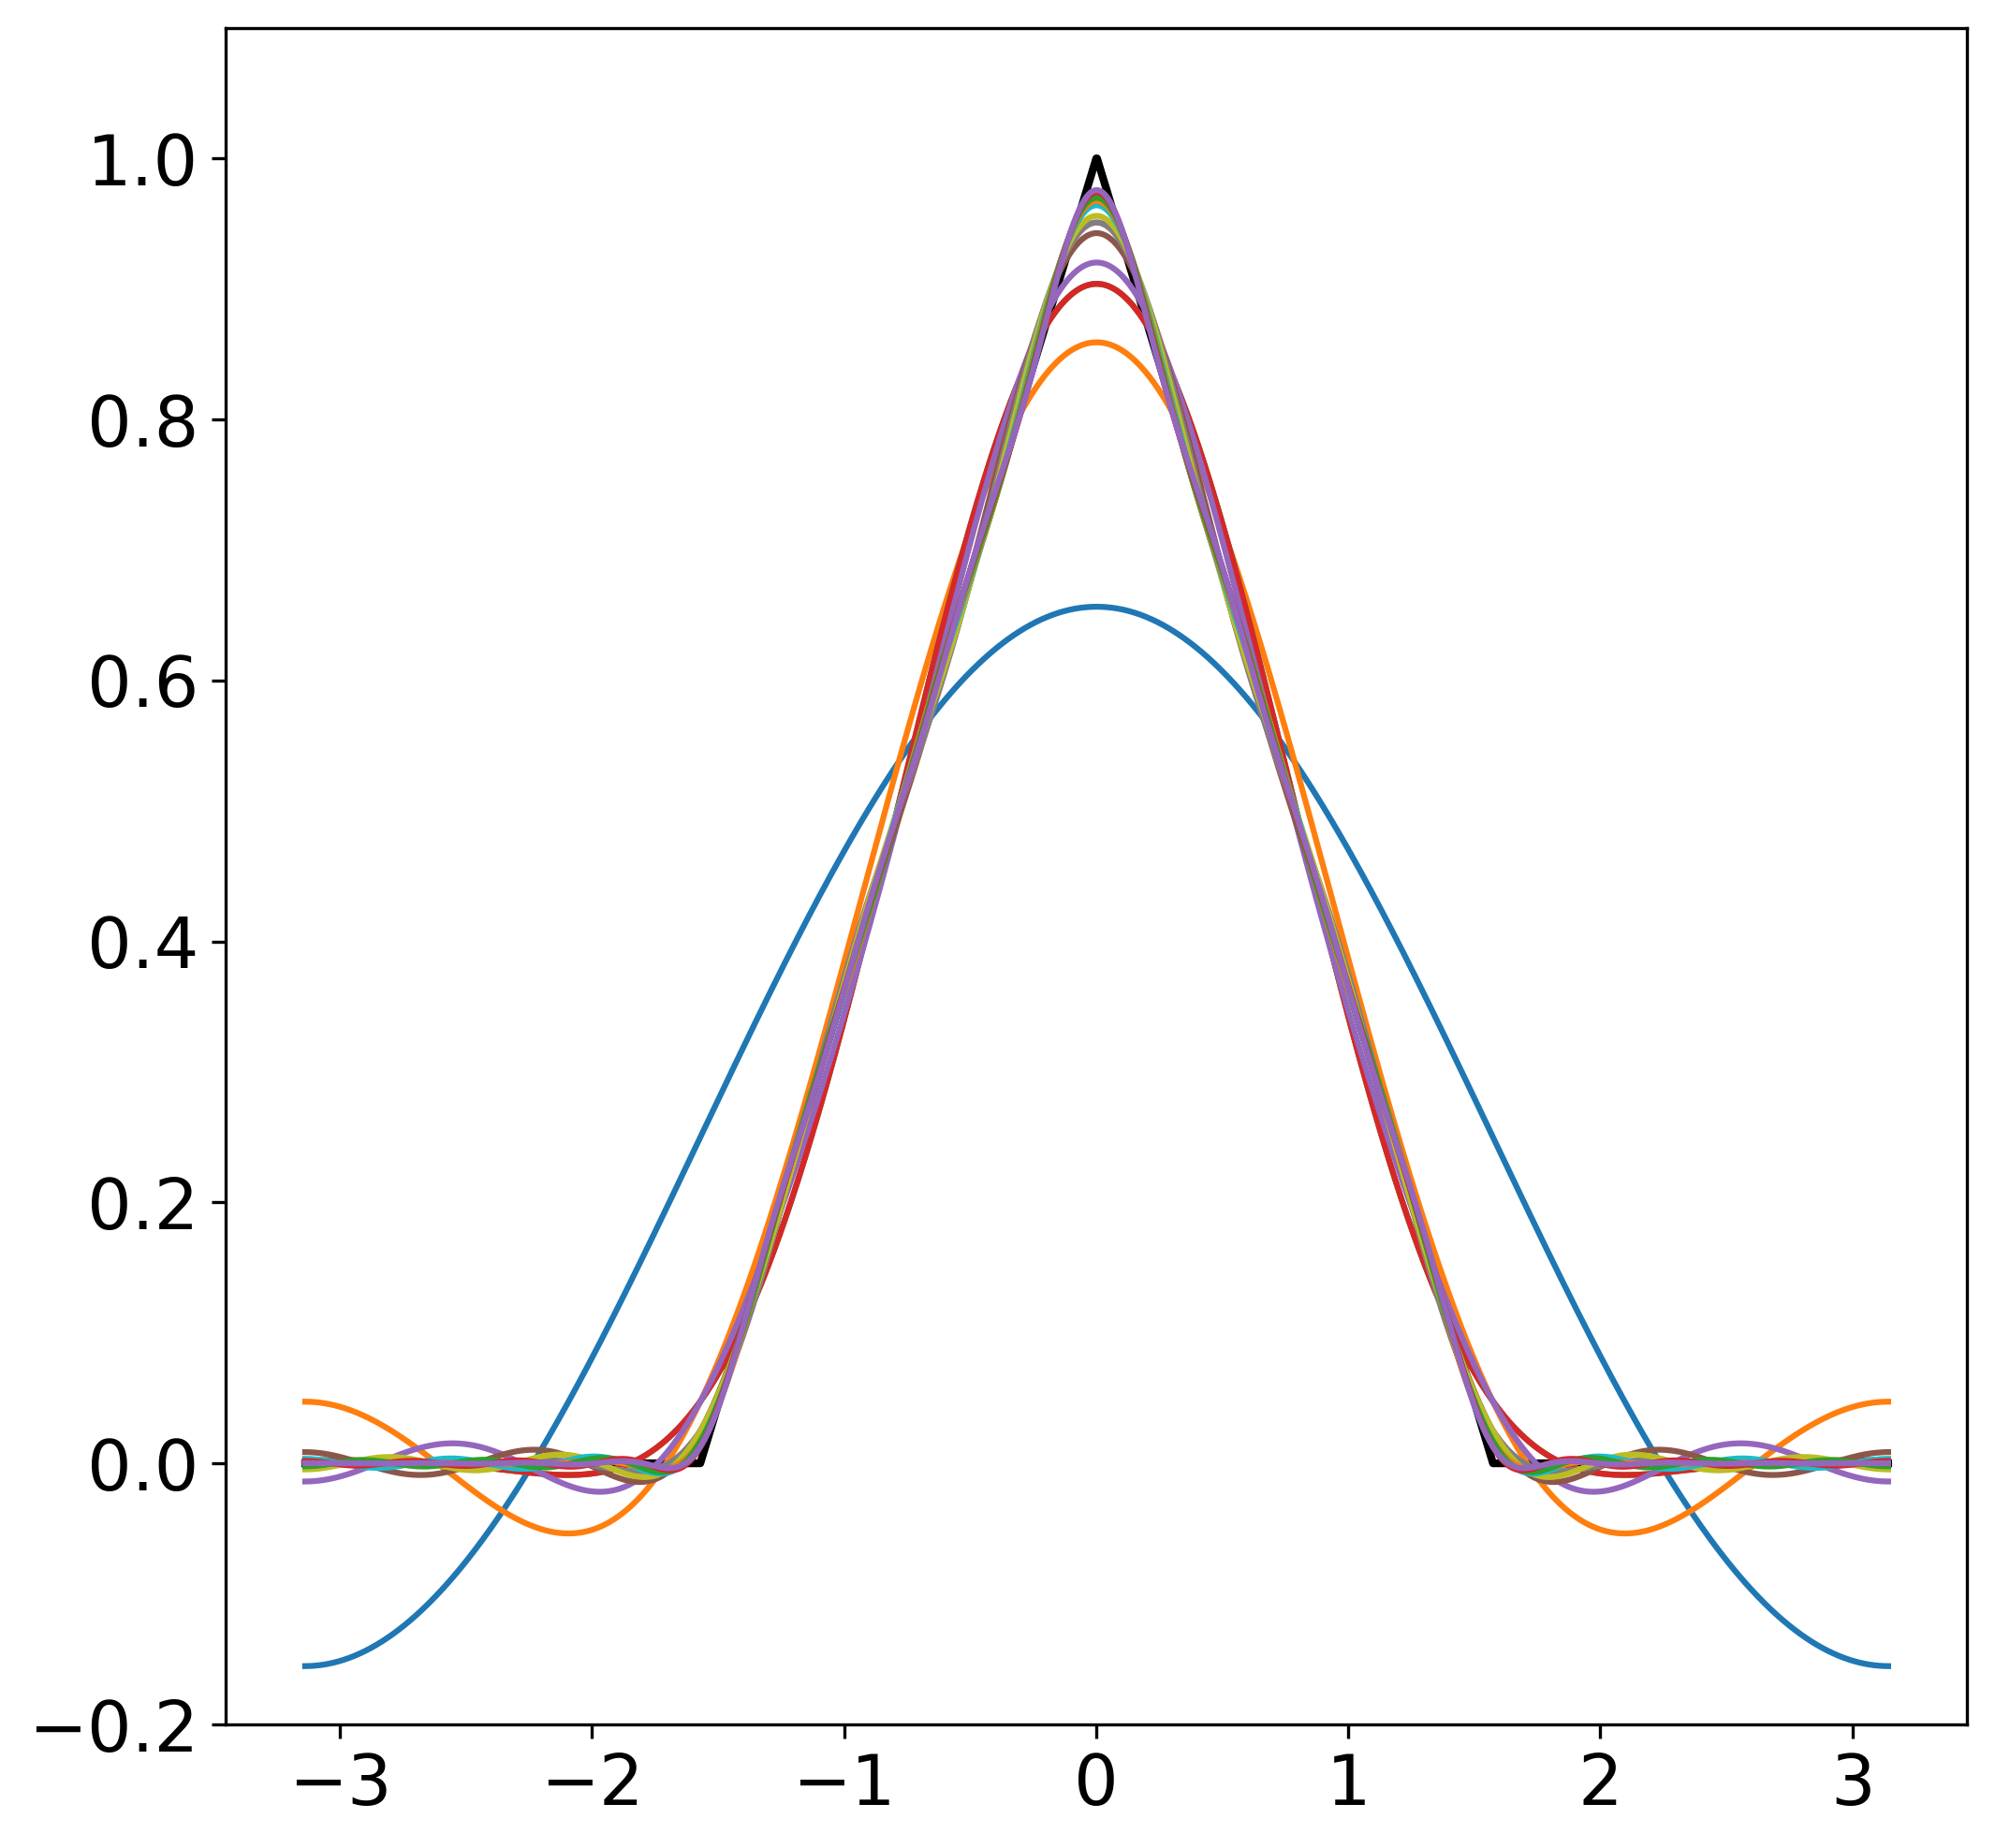
\includegraphics[width=.5\linewidth]{programs/fourier1/out_15.png}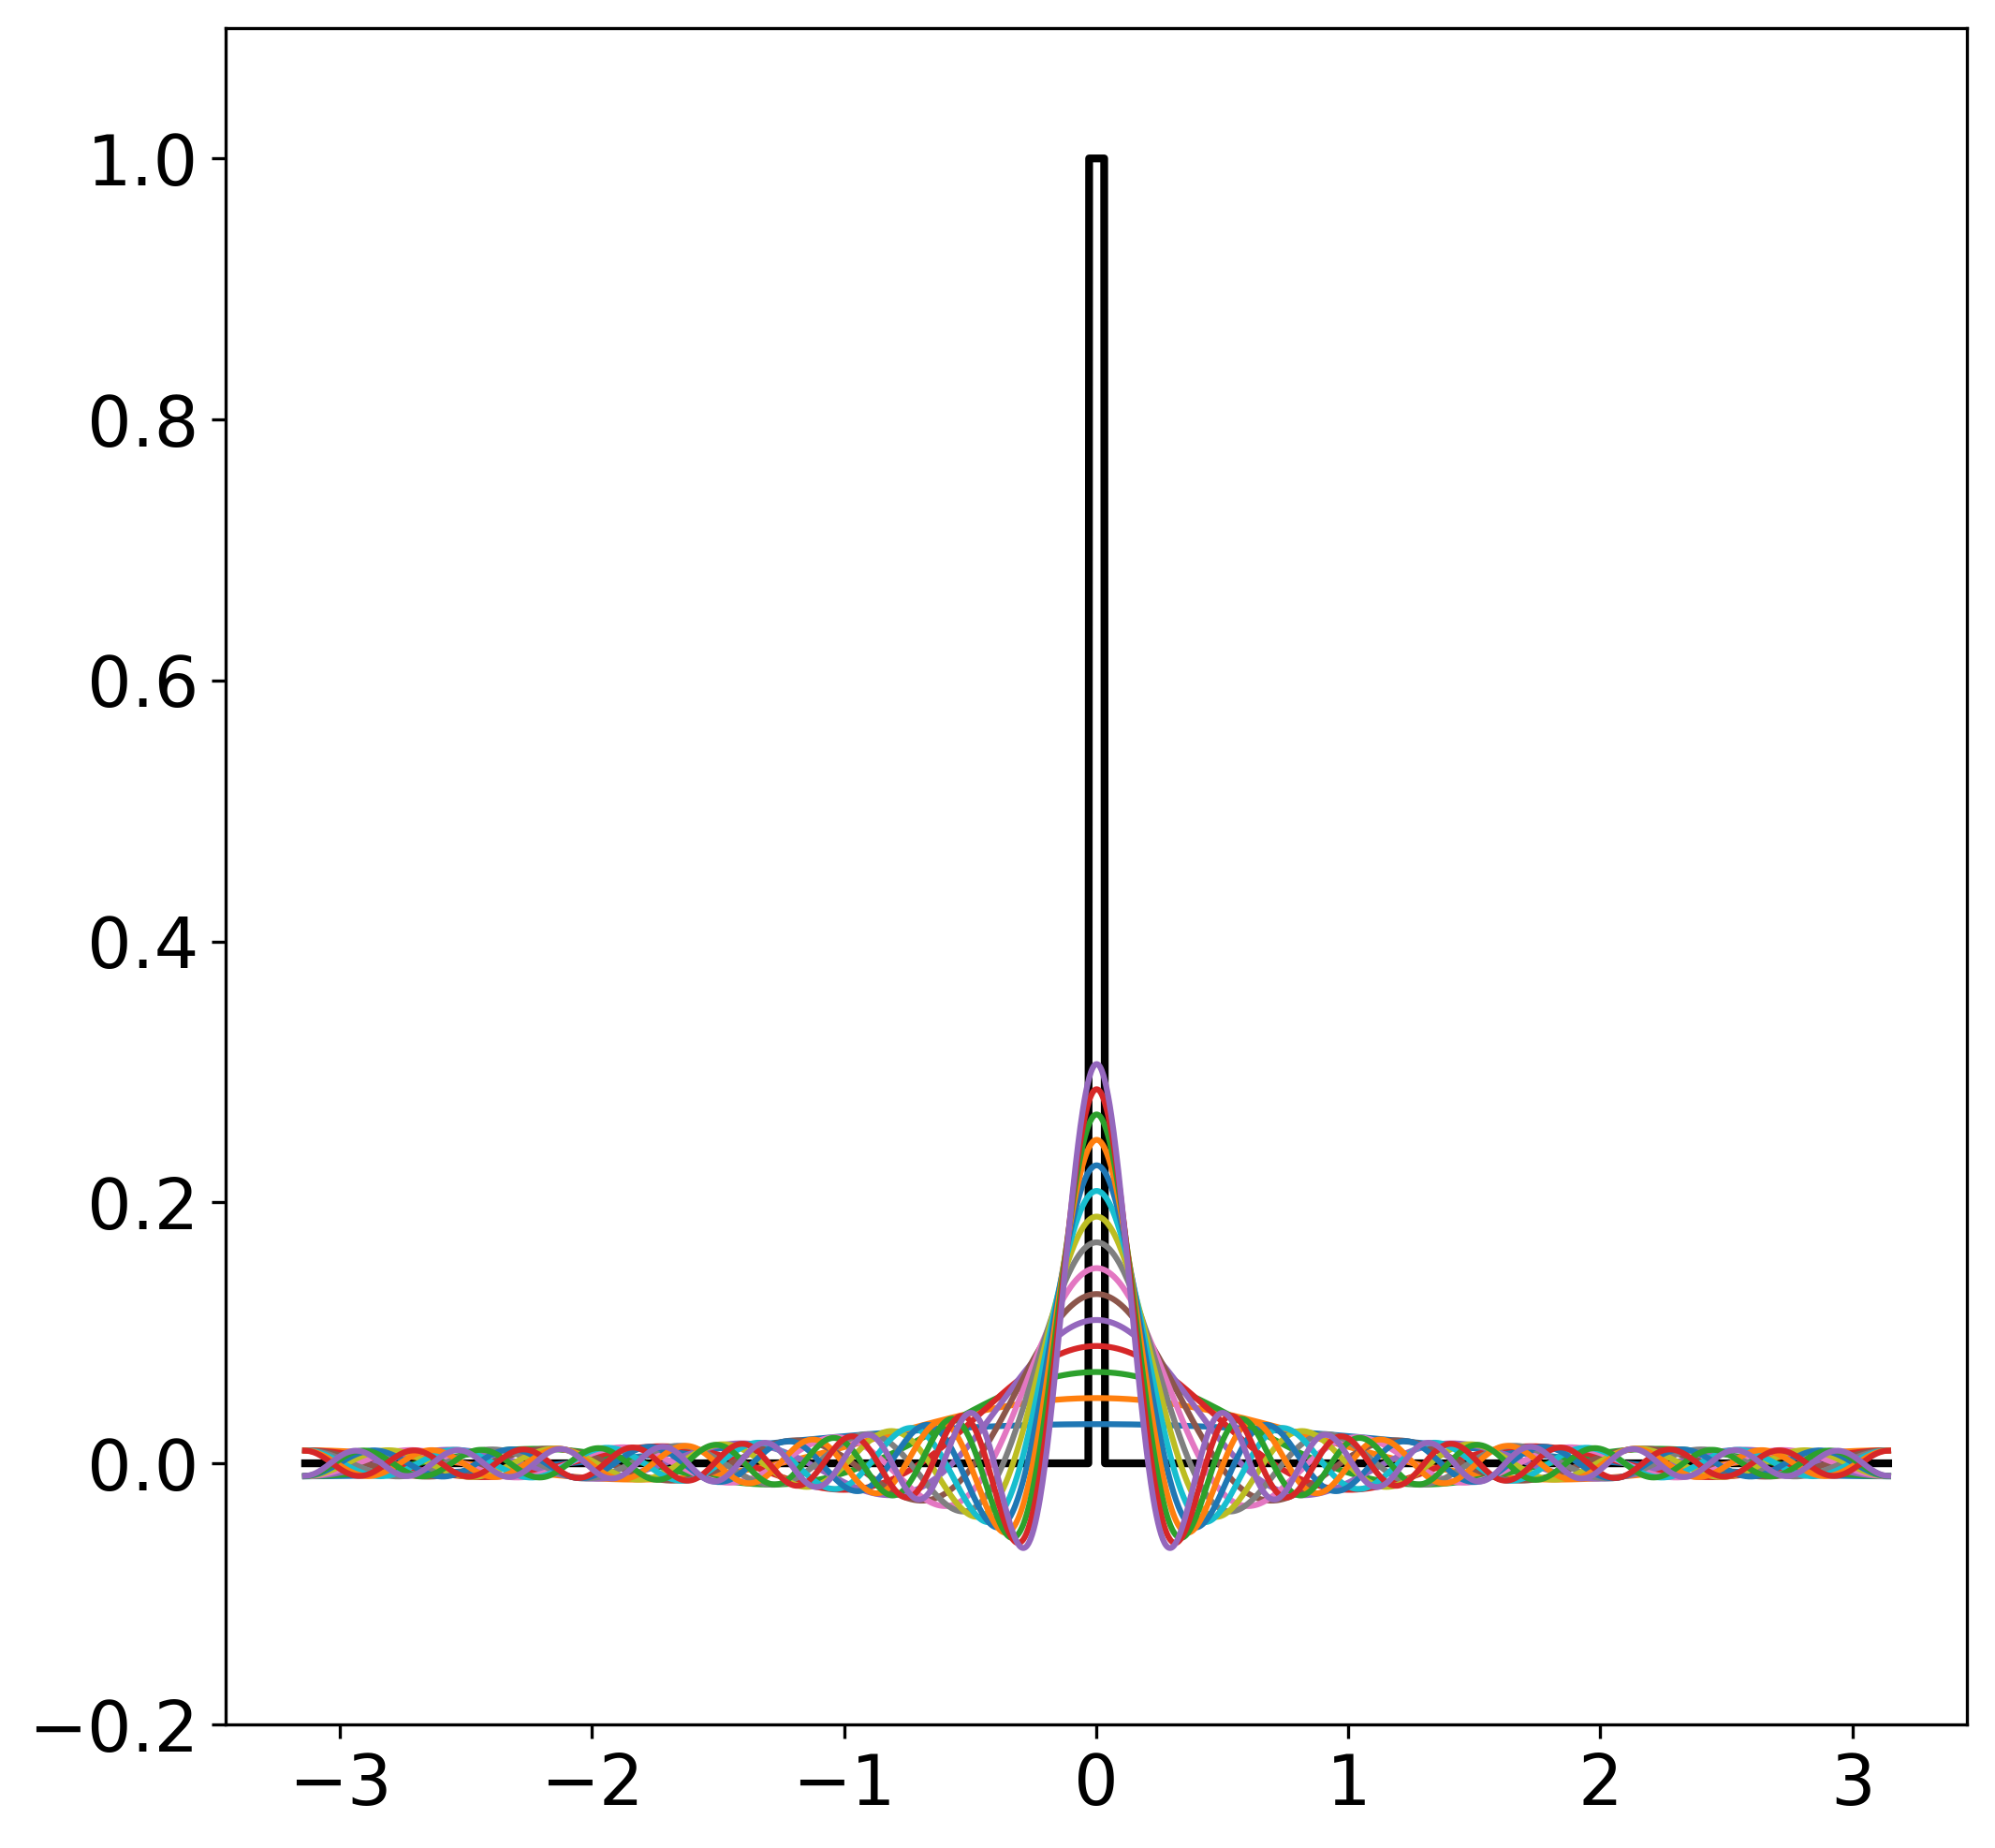
\includegraphics[width=.5\linewidth]{programs/fourier2/out_15.png}}
    \only<17|handout:0>{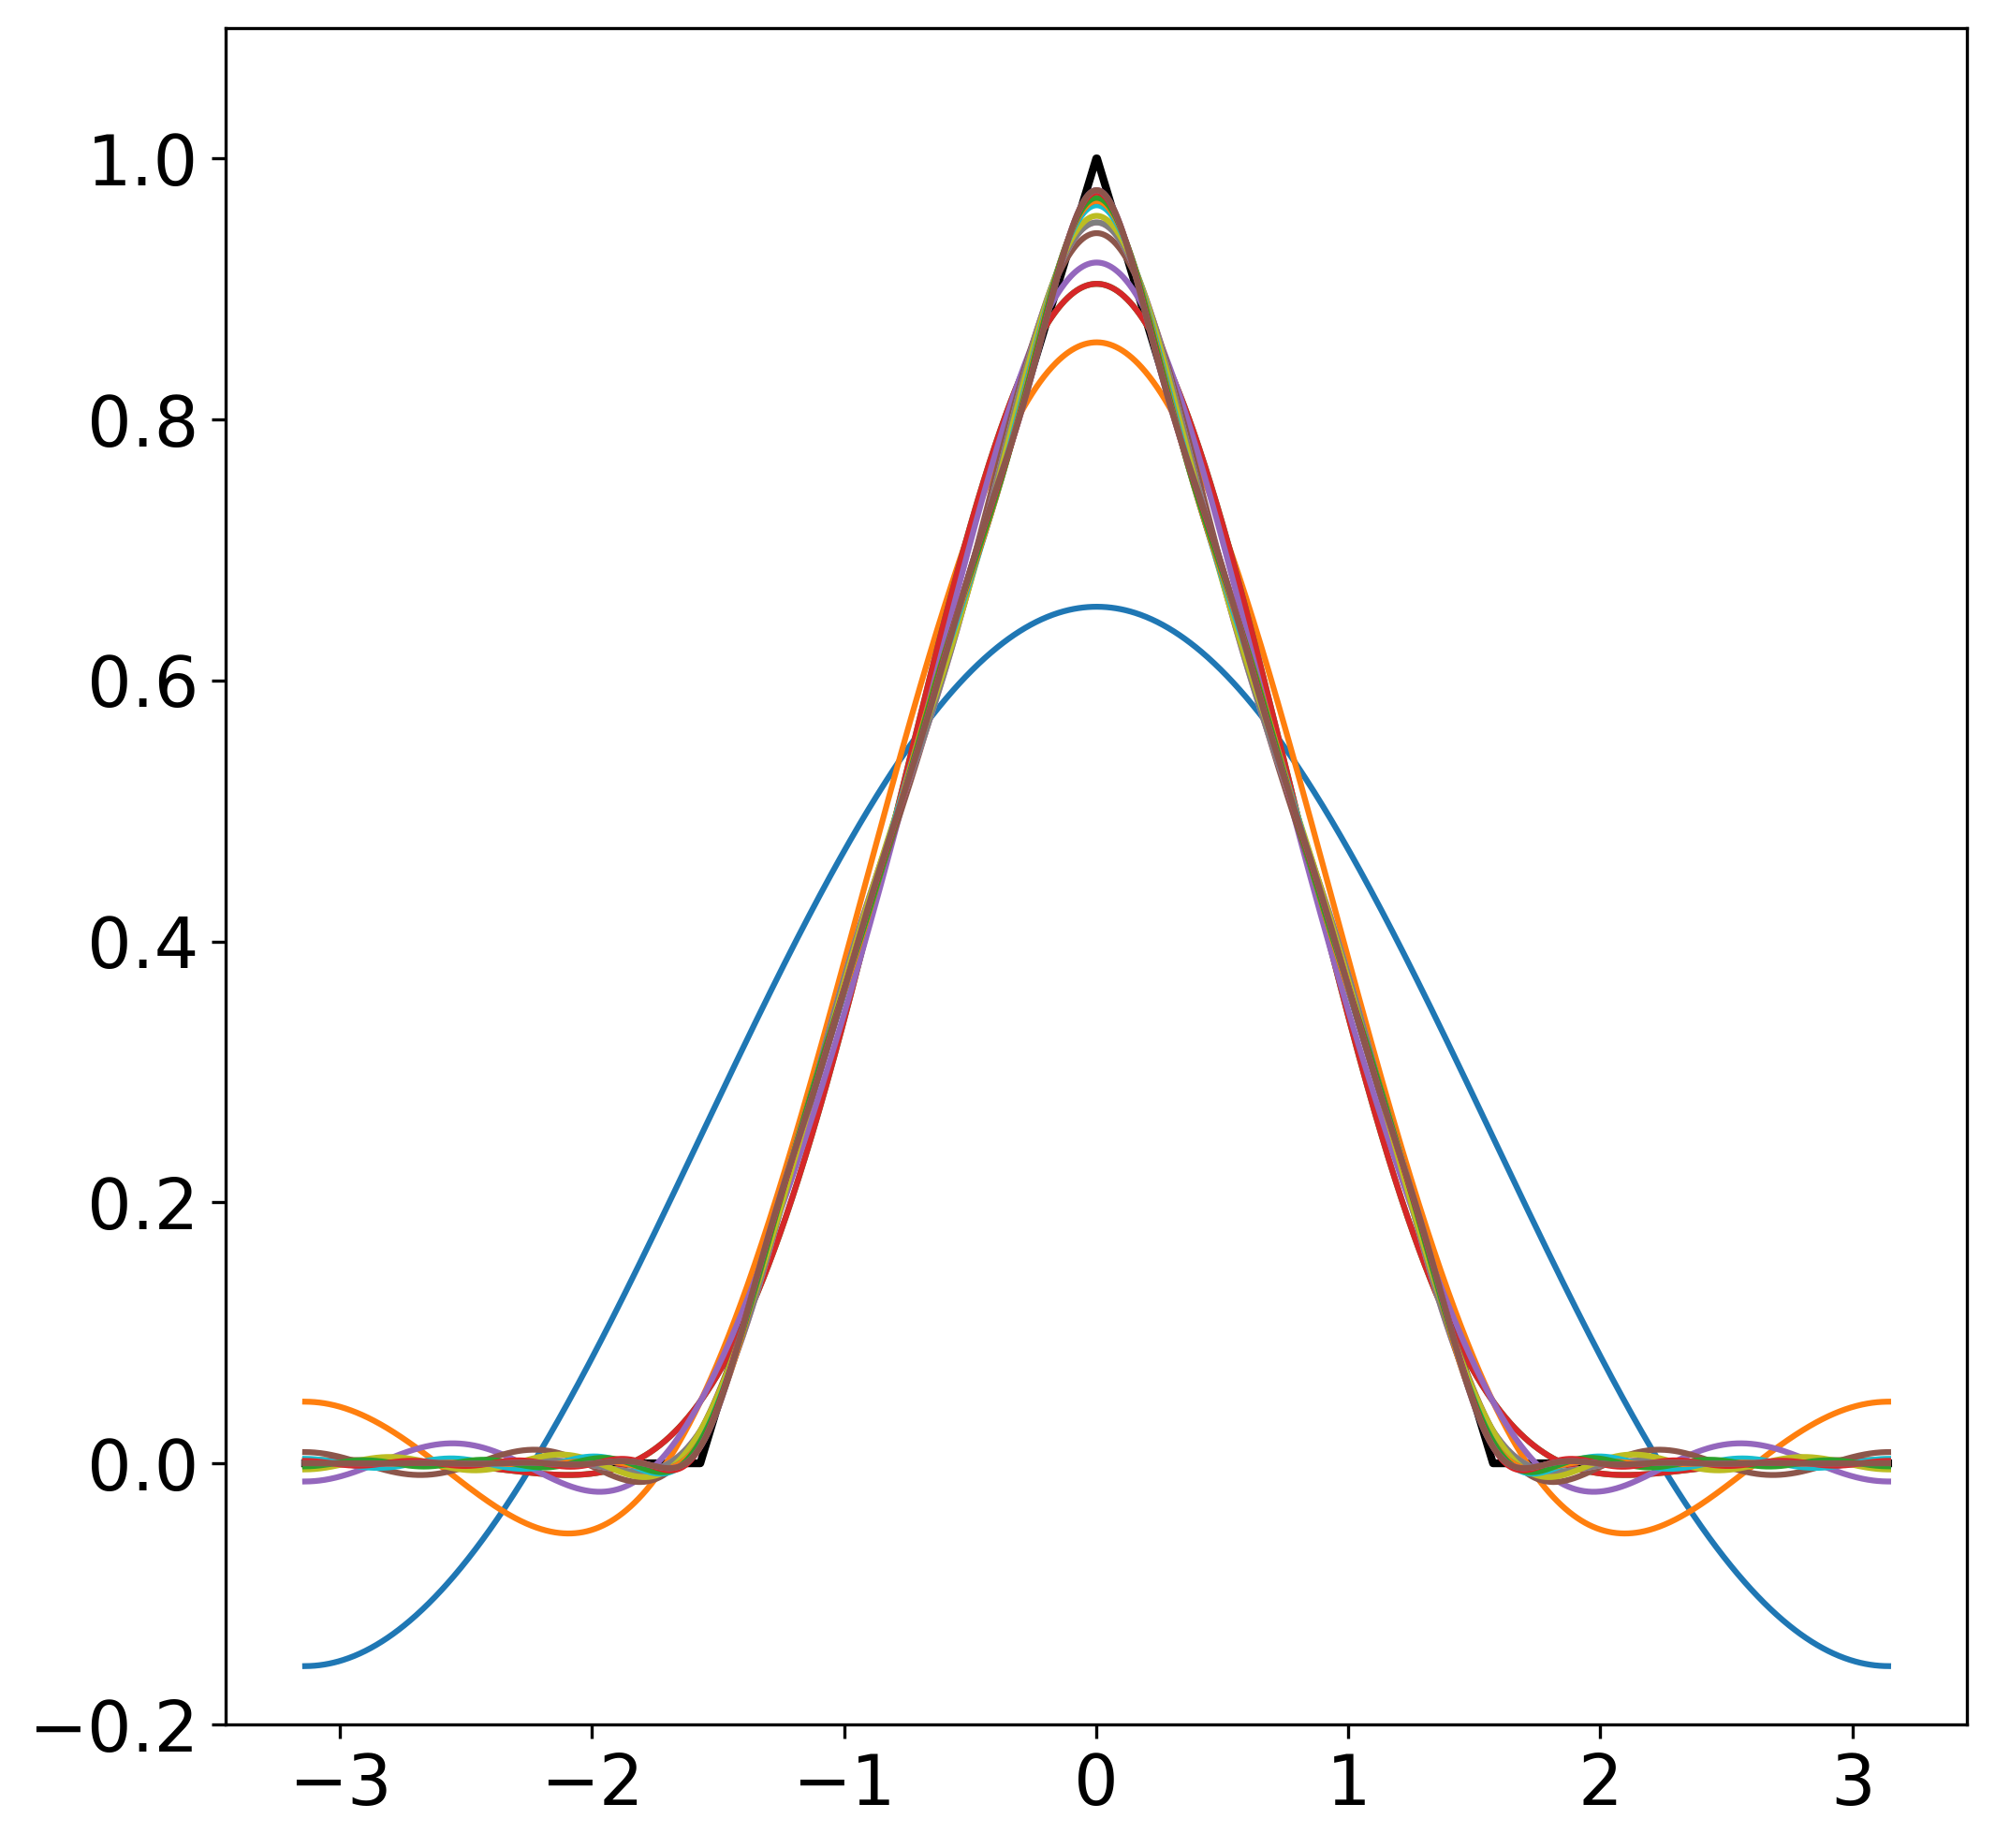
\includegraphics[width=.5\linewidth]{programs/fourier1/out_16.png}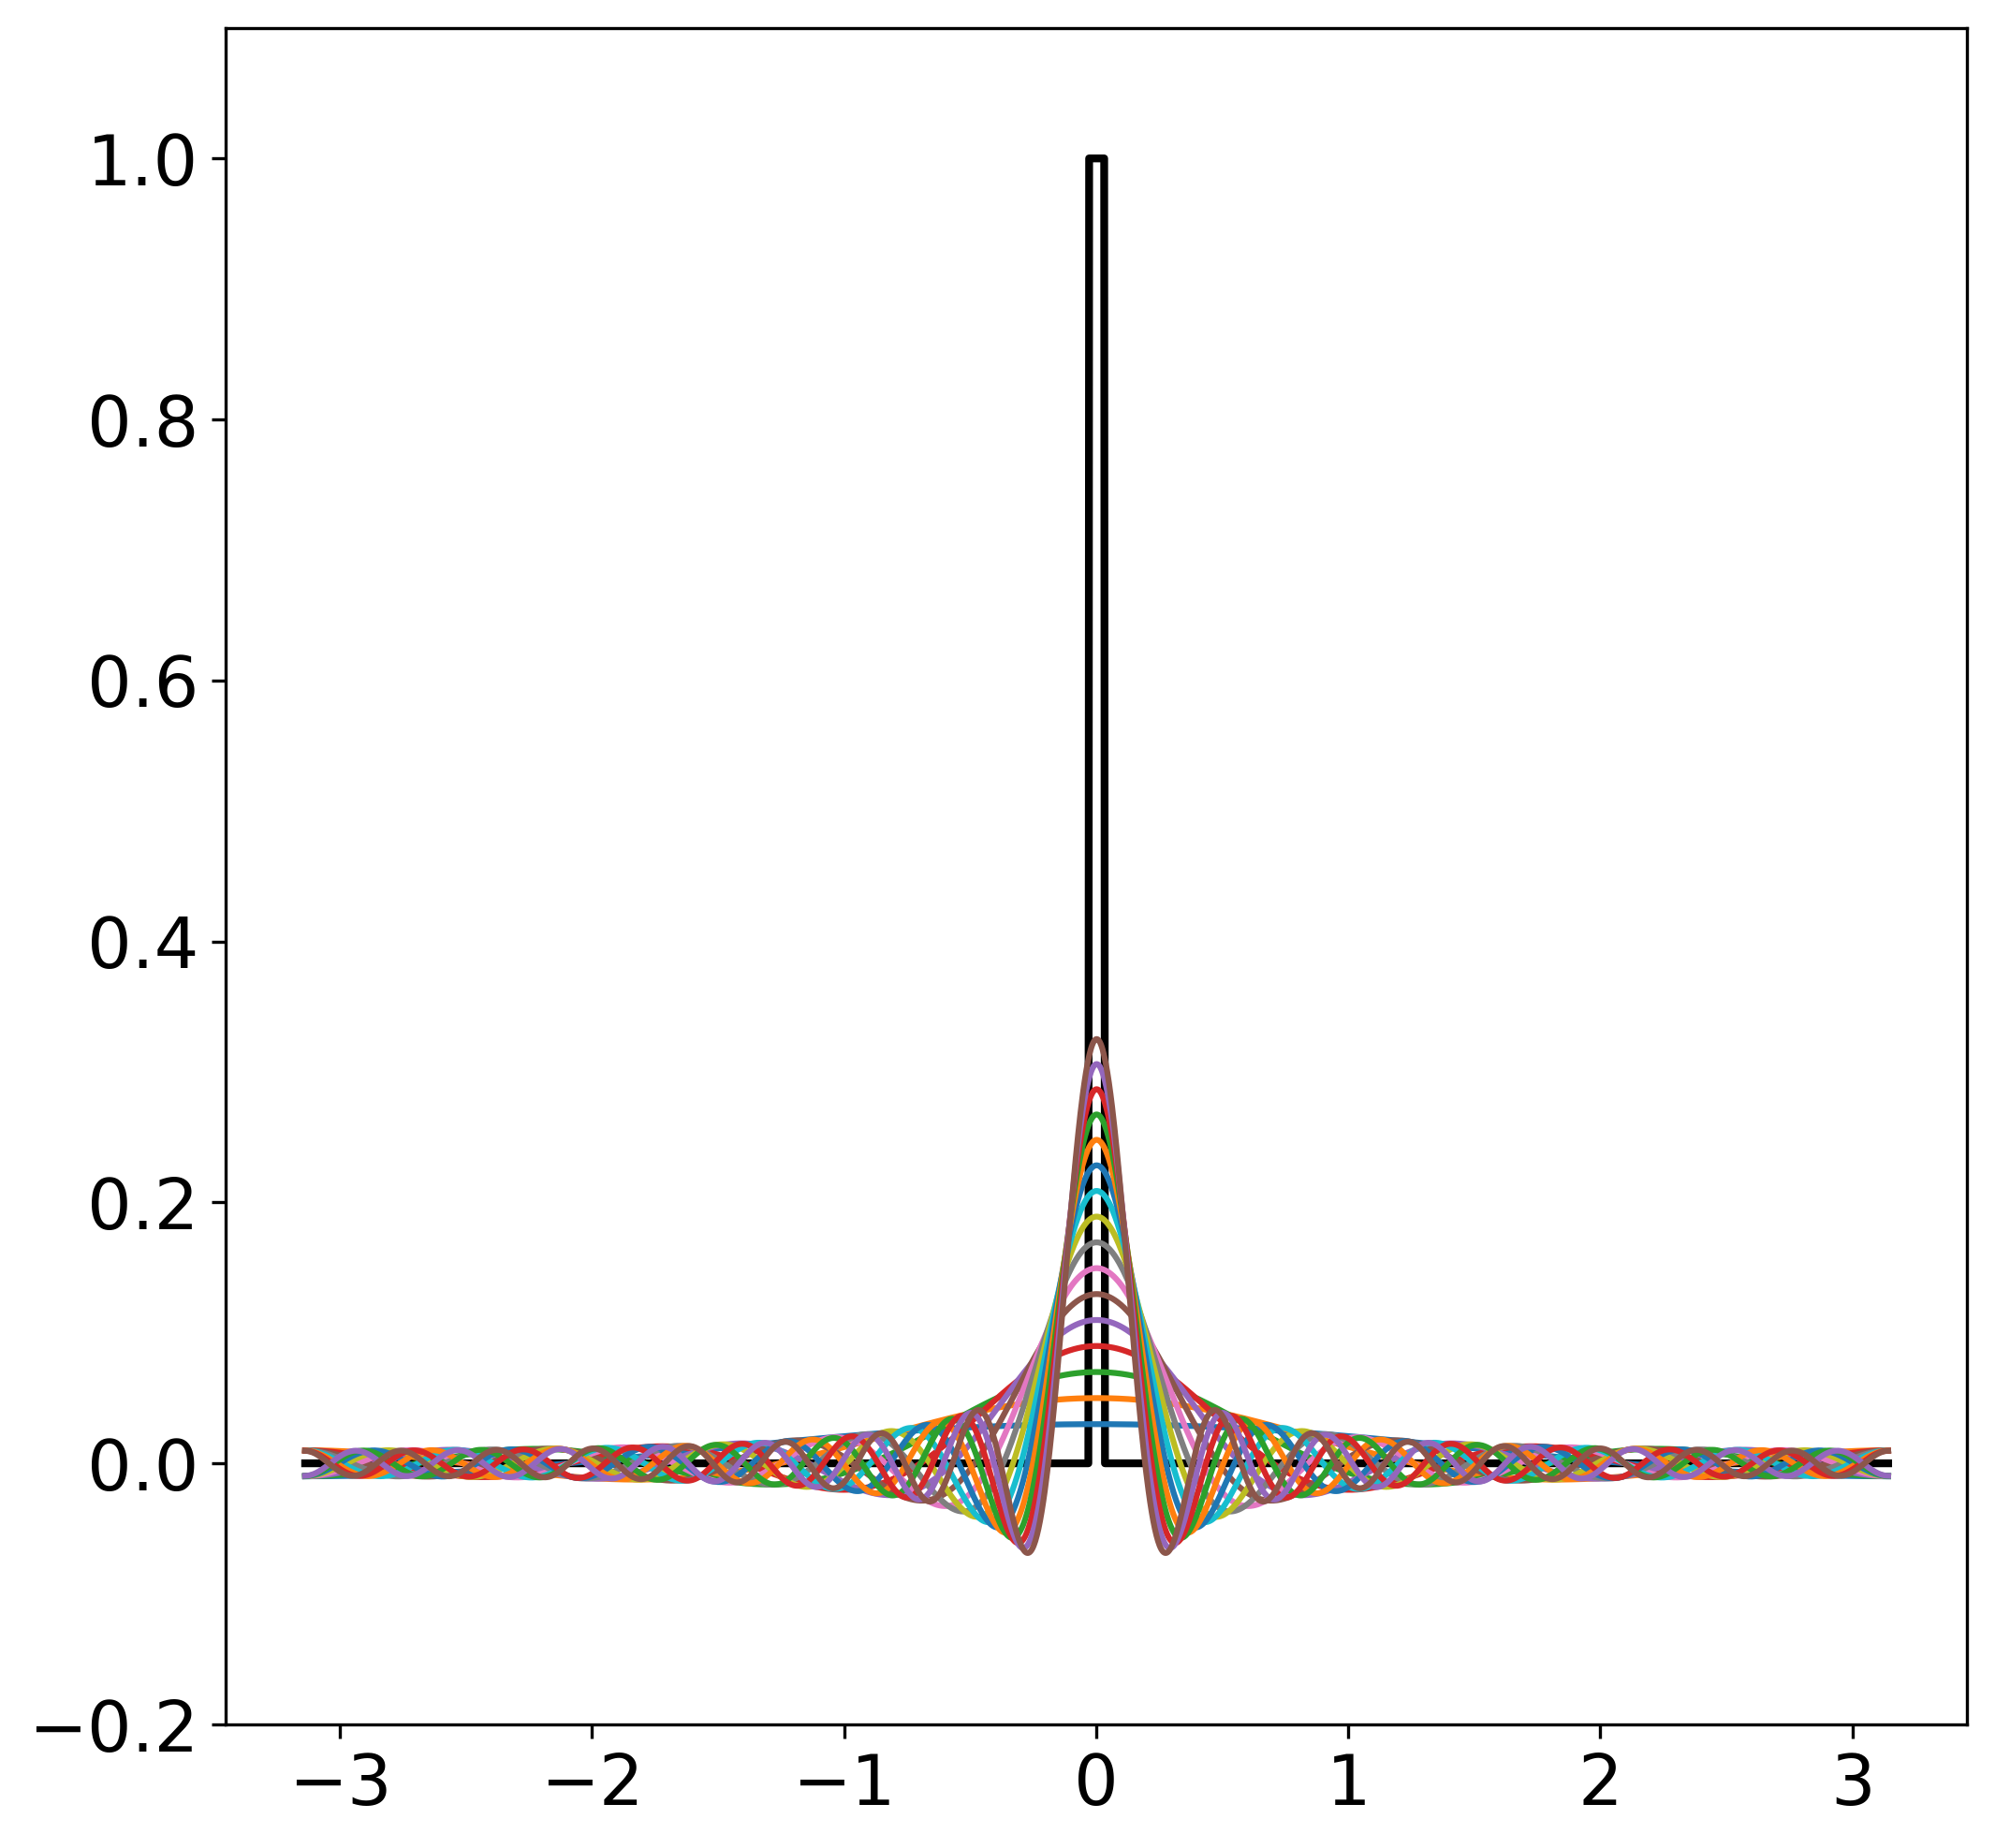
\includegraphics[width=.5\linewidth]{programs/fourier2/out_16.png}}
    \only<18|handout:0>{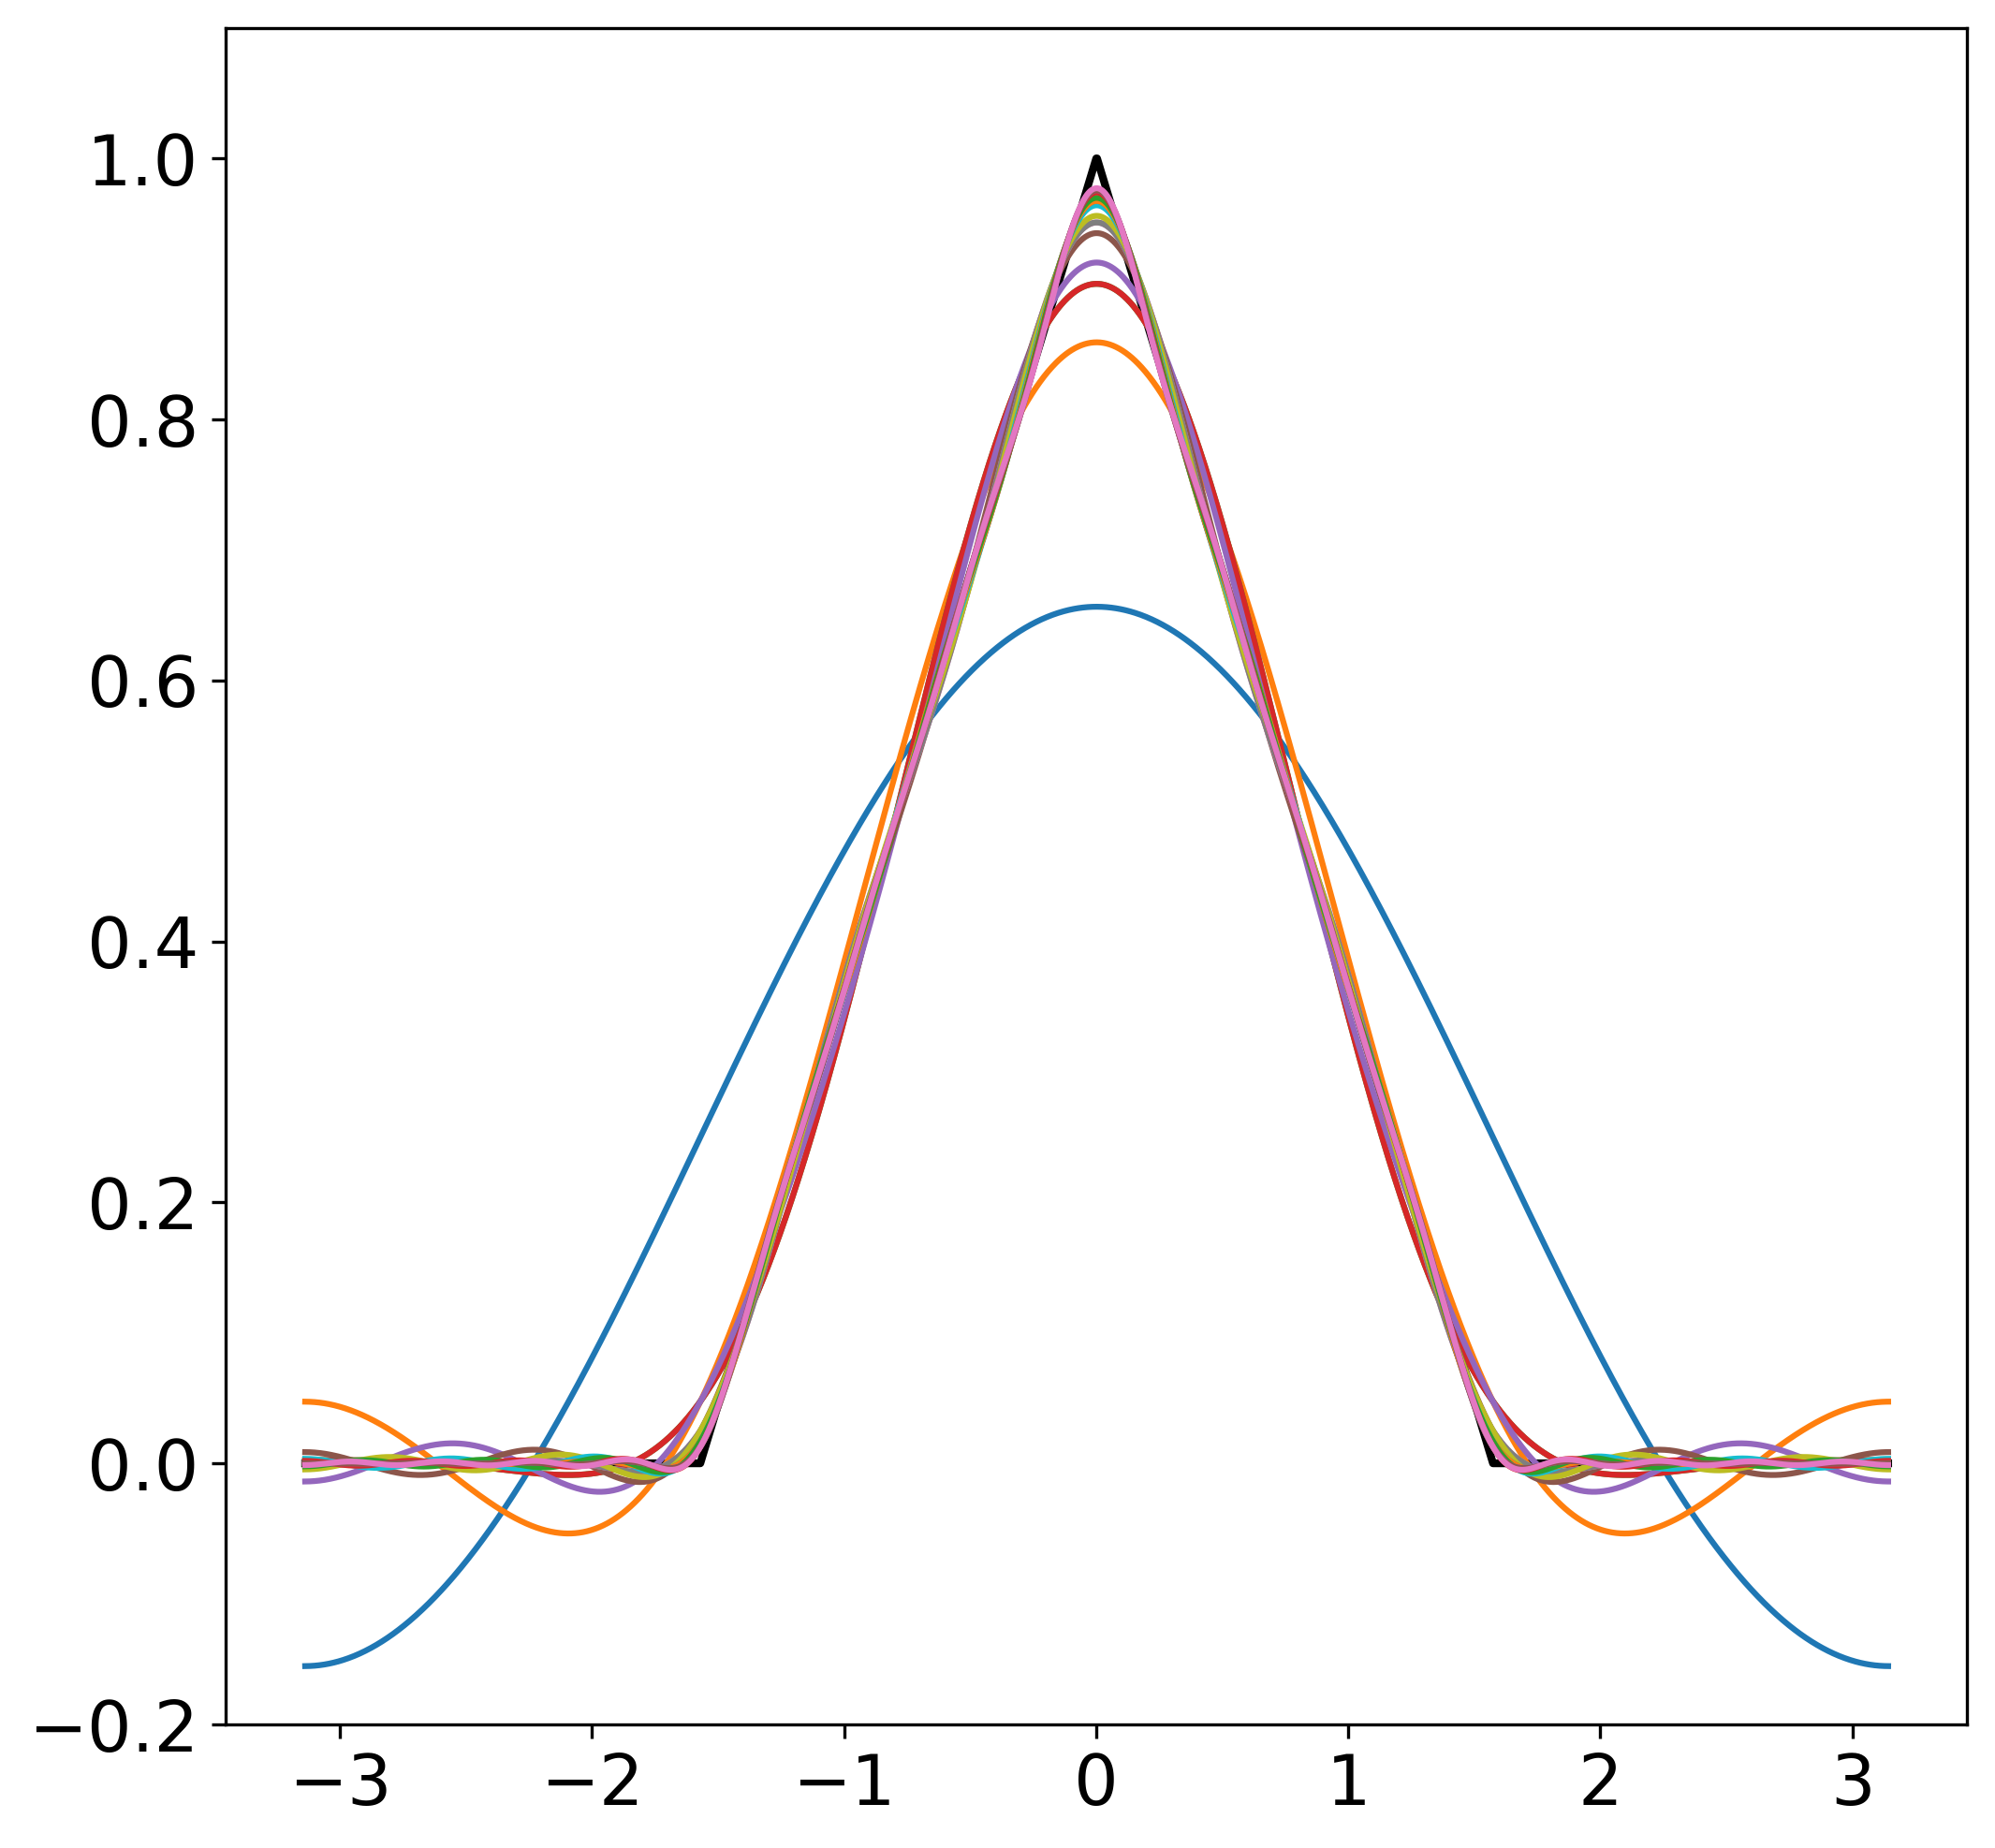
\includegraphics[width=.5\linewidth]{programs/fourier1/out_17.png}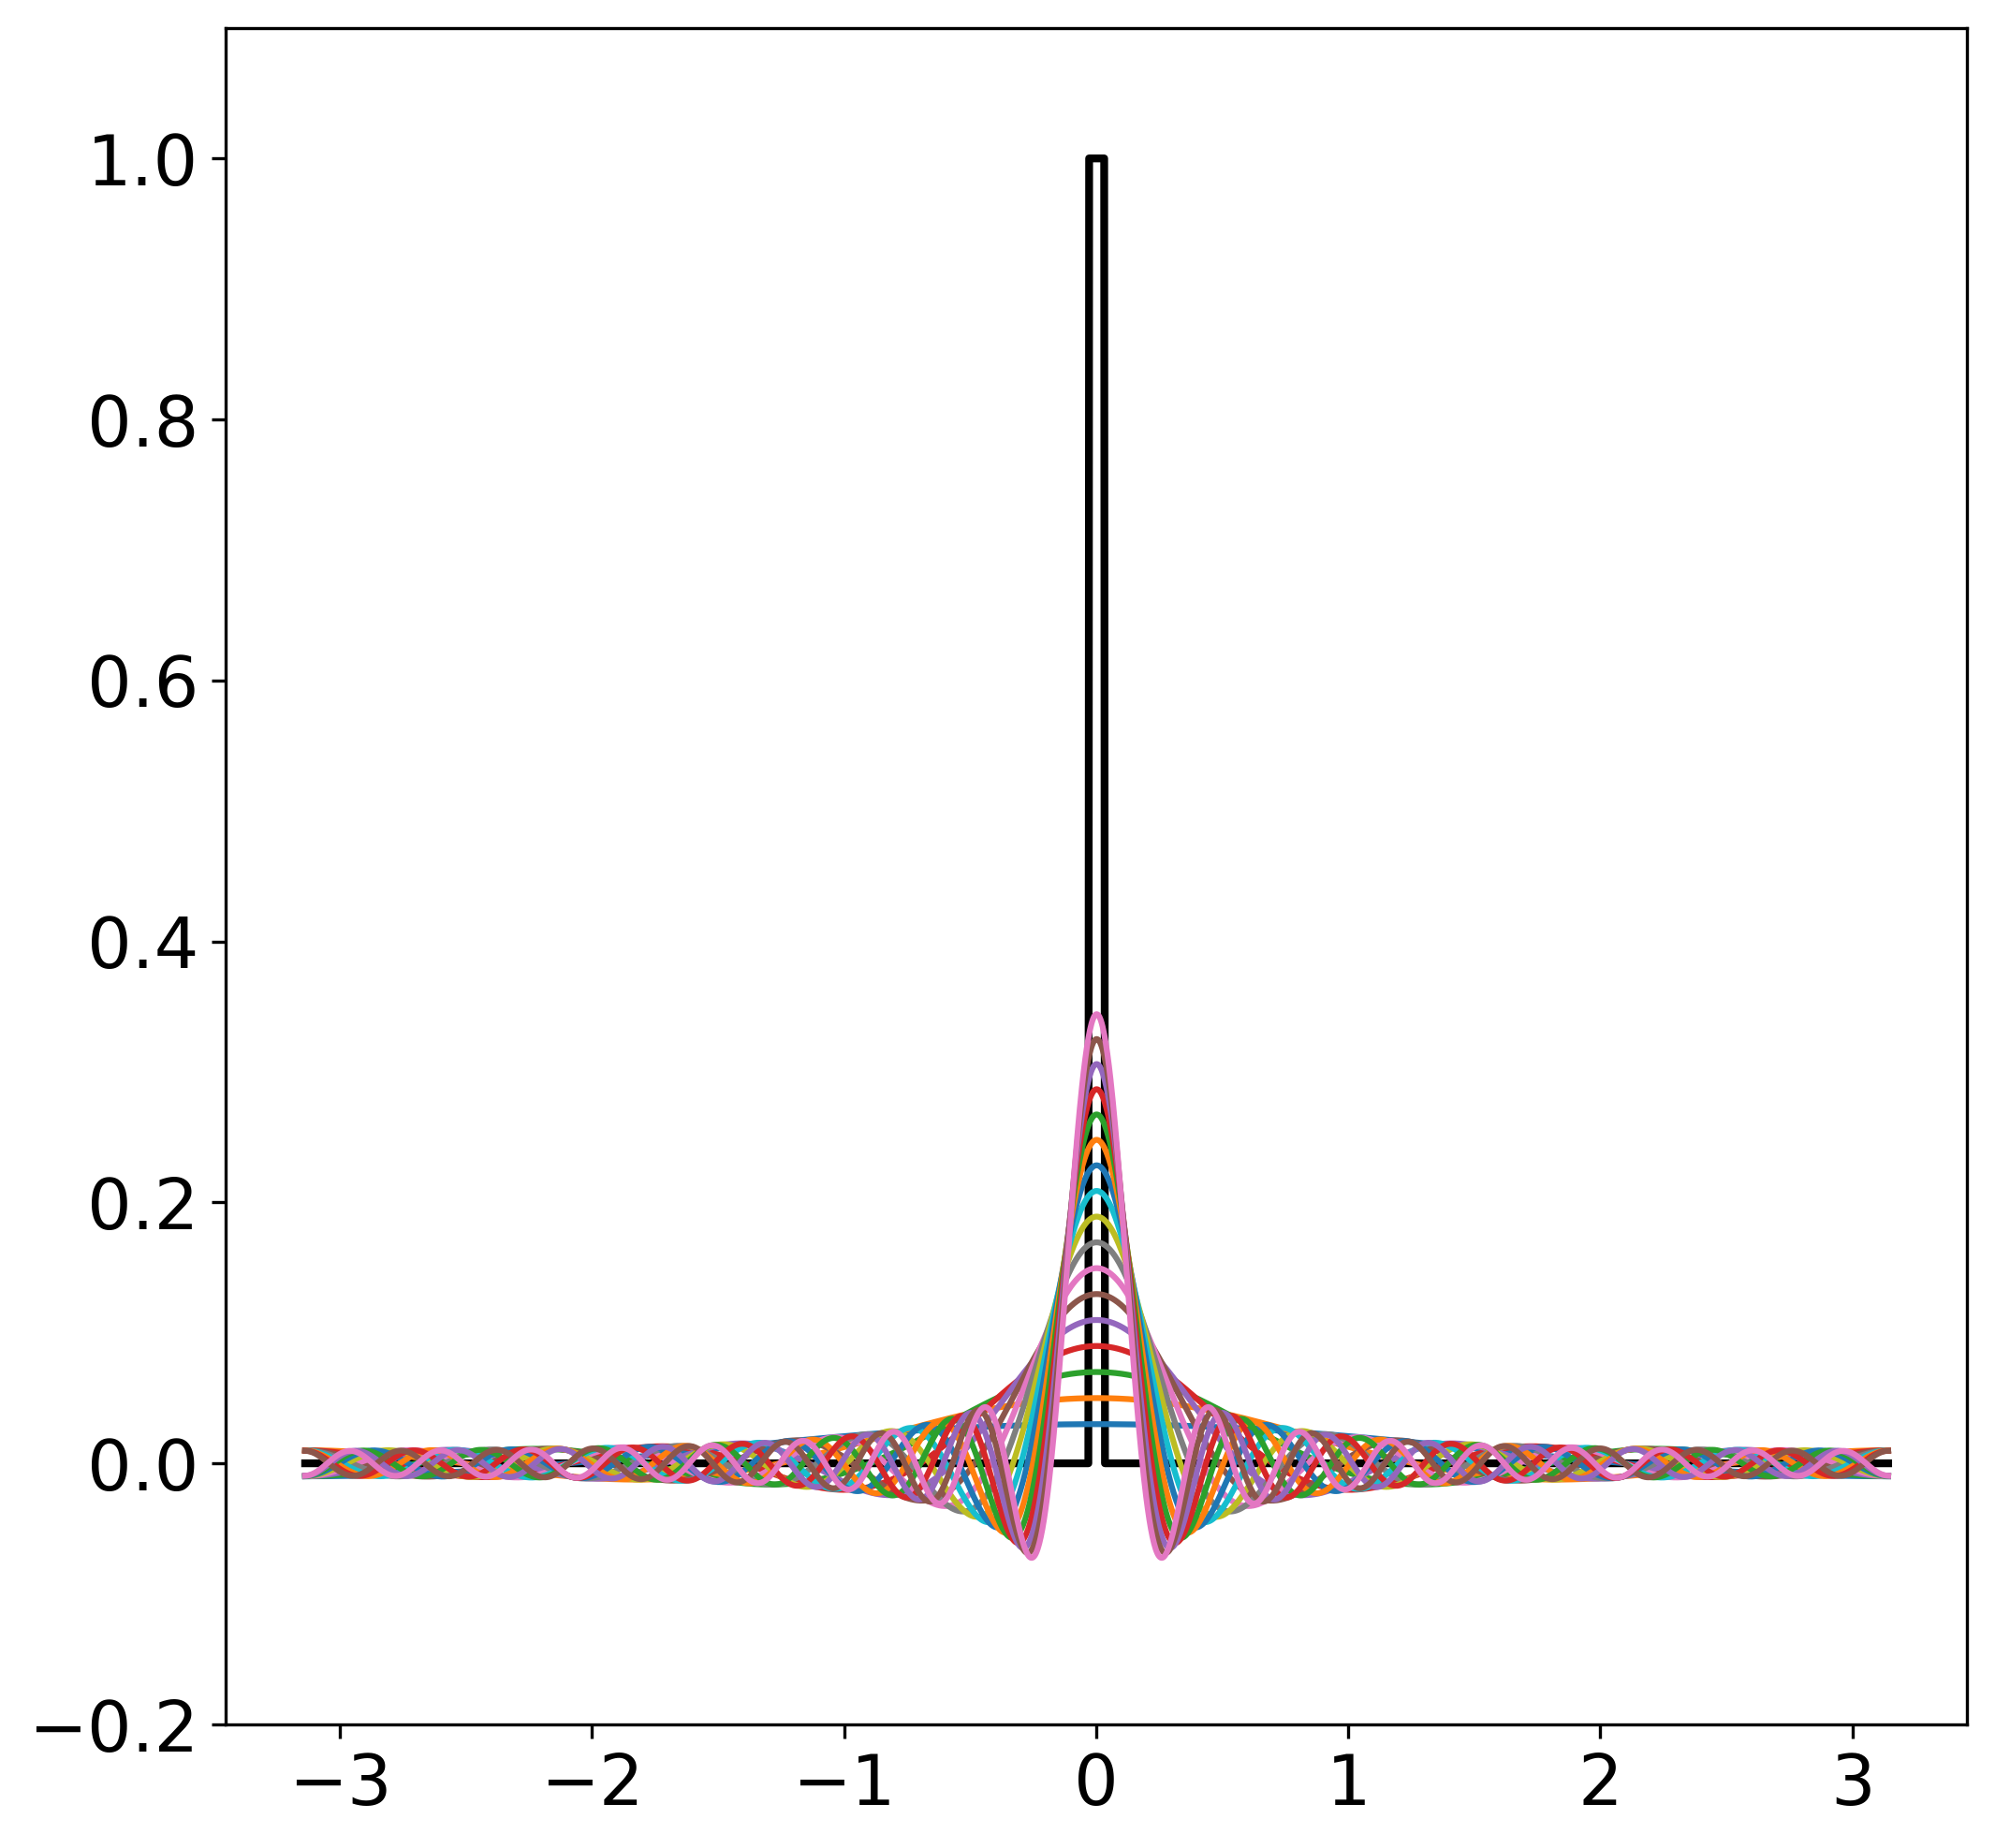
\includegraphics[width=.5\linewidth]{programs/fourier2/out_17.png}}
    \only<19|handout:0>{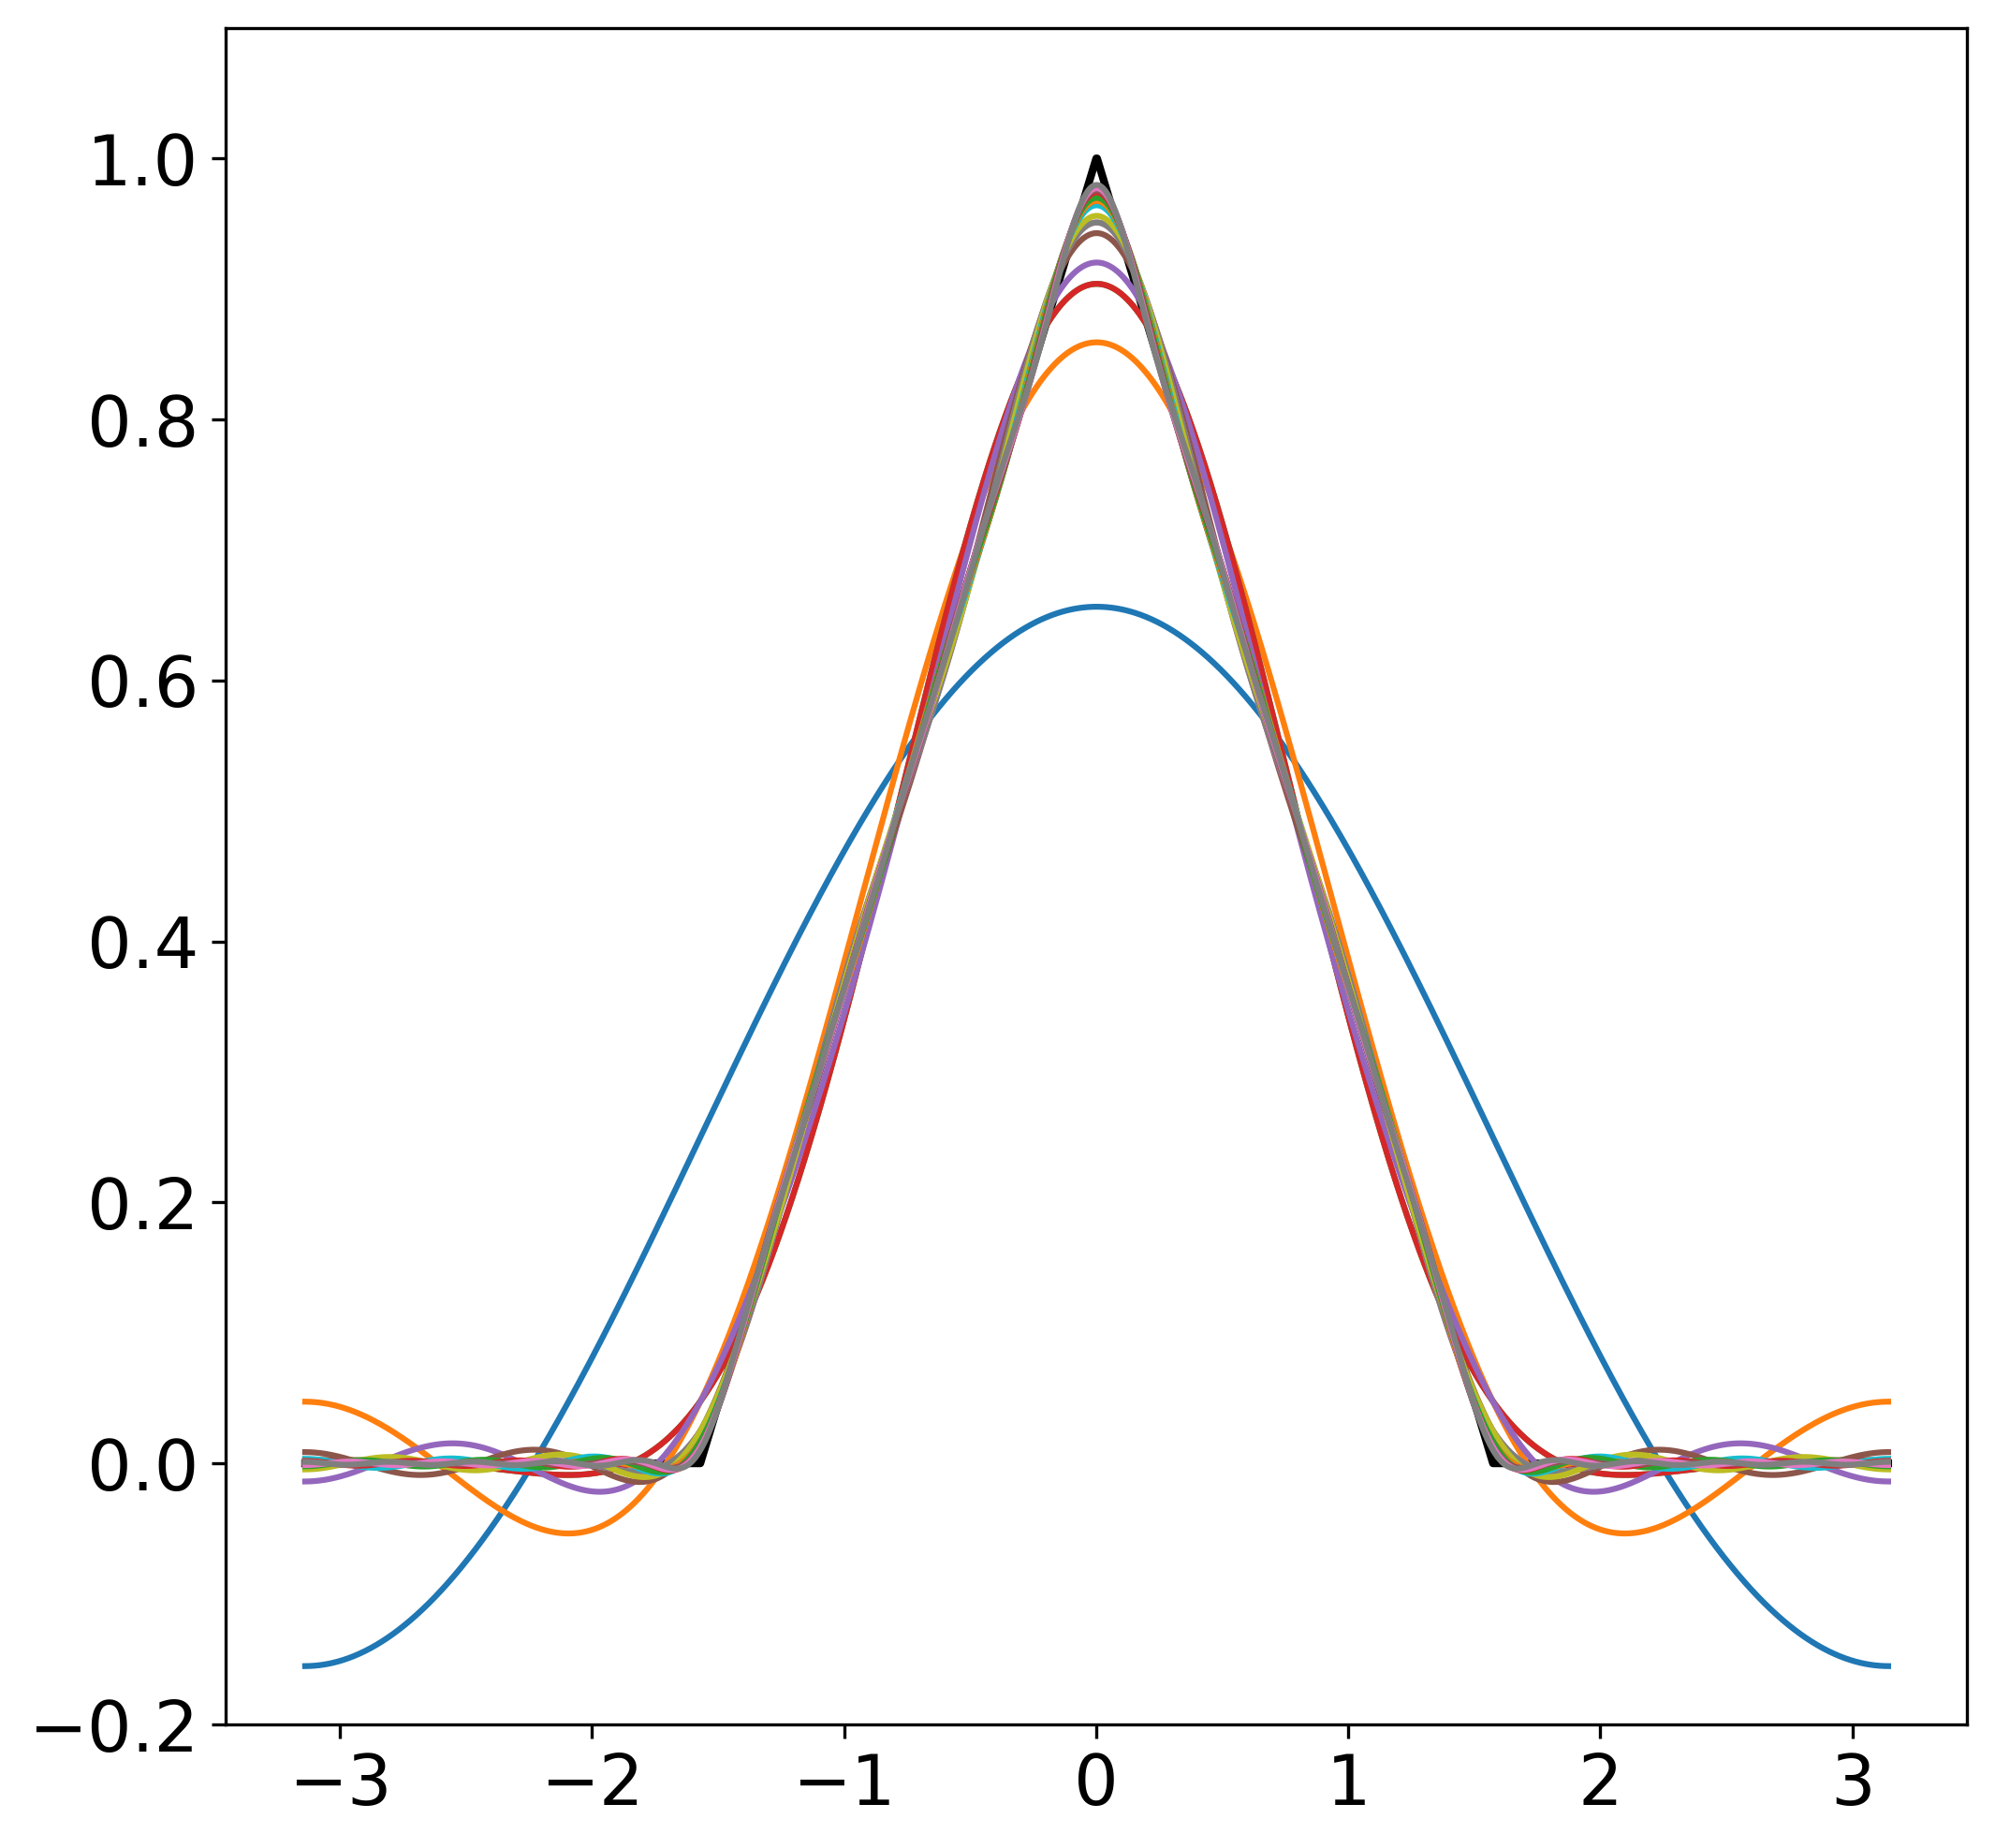
\includegraphics[width=.5\linewidth]{programs/fourier1/out_18.png}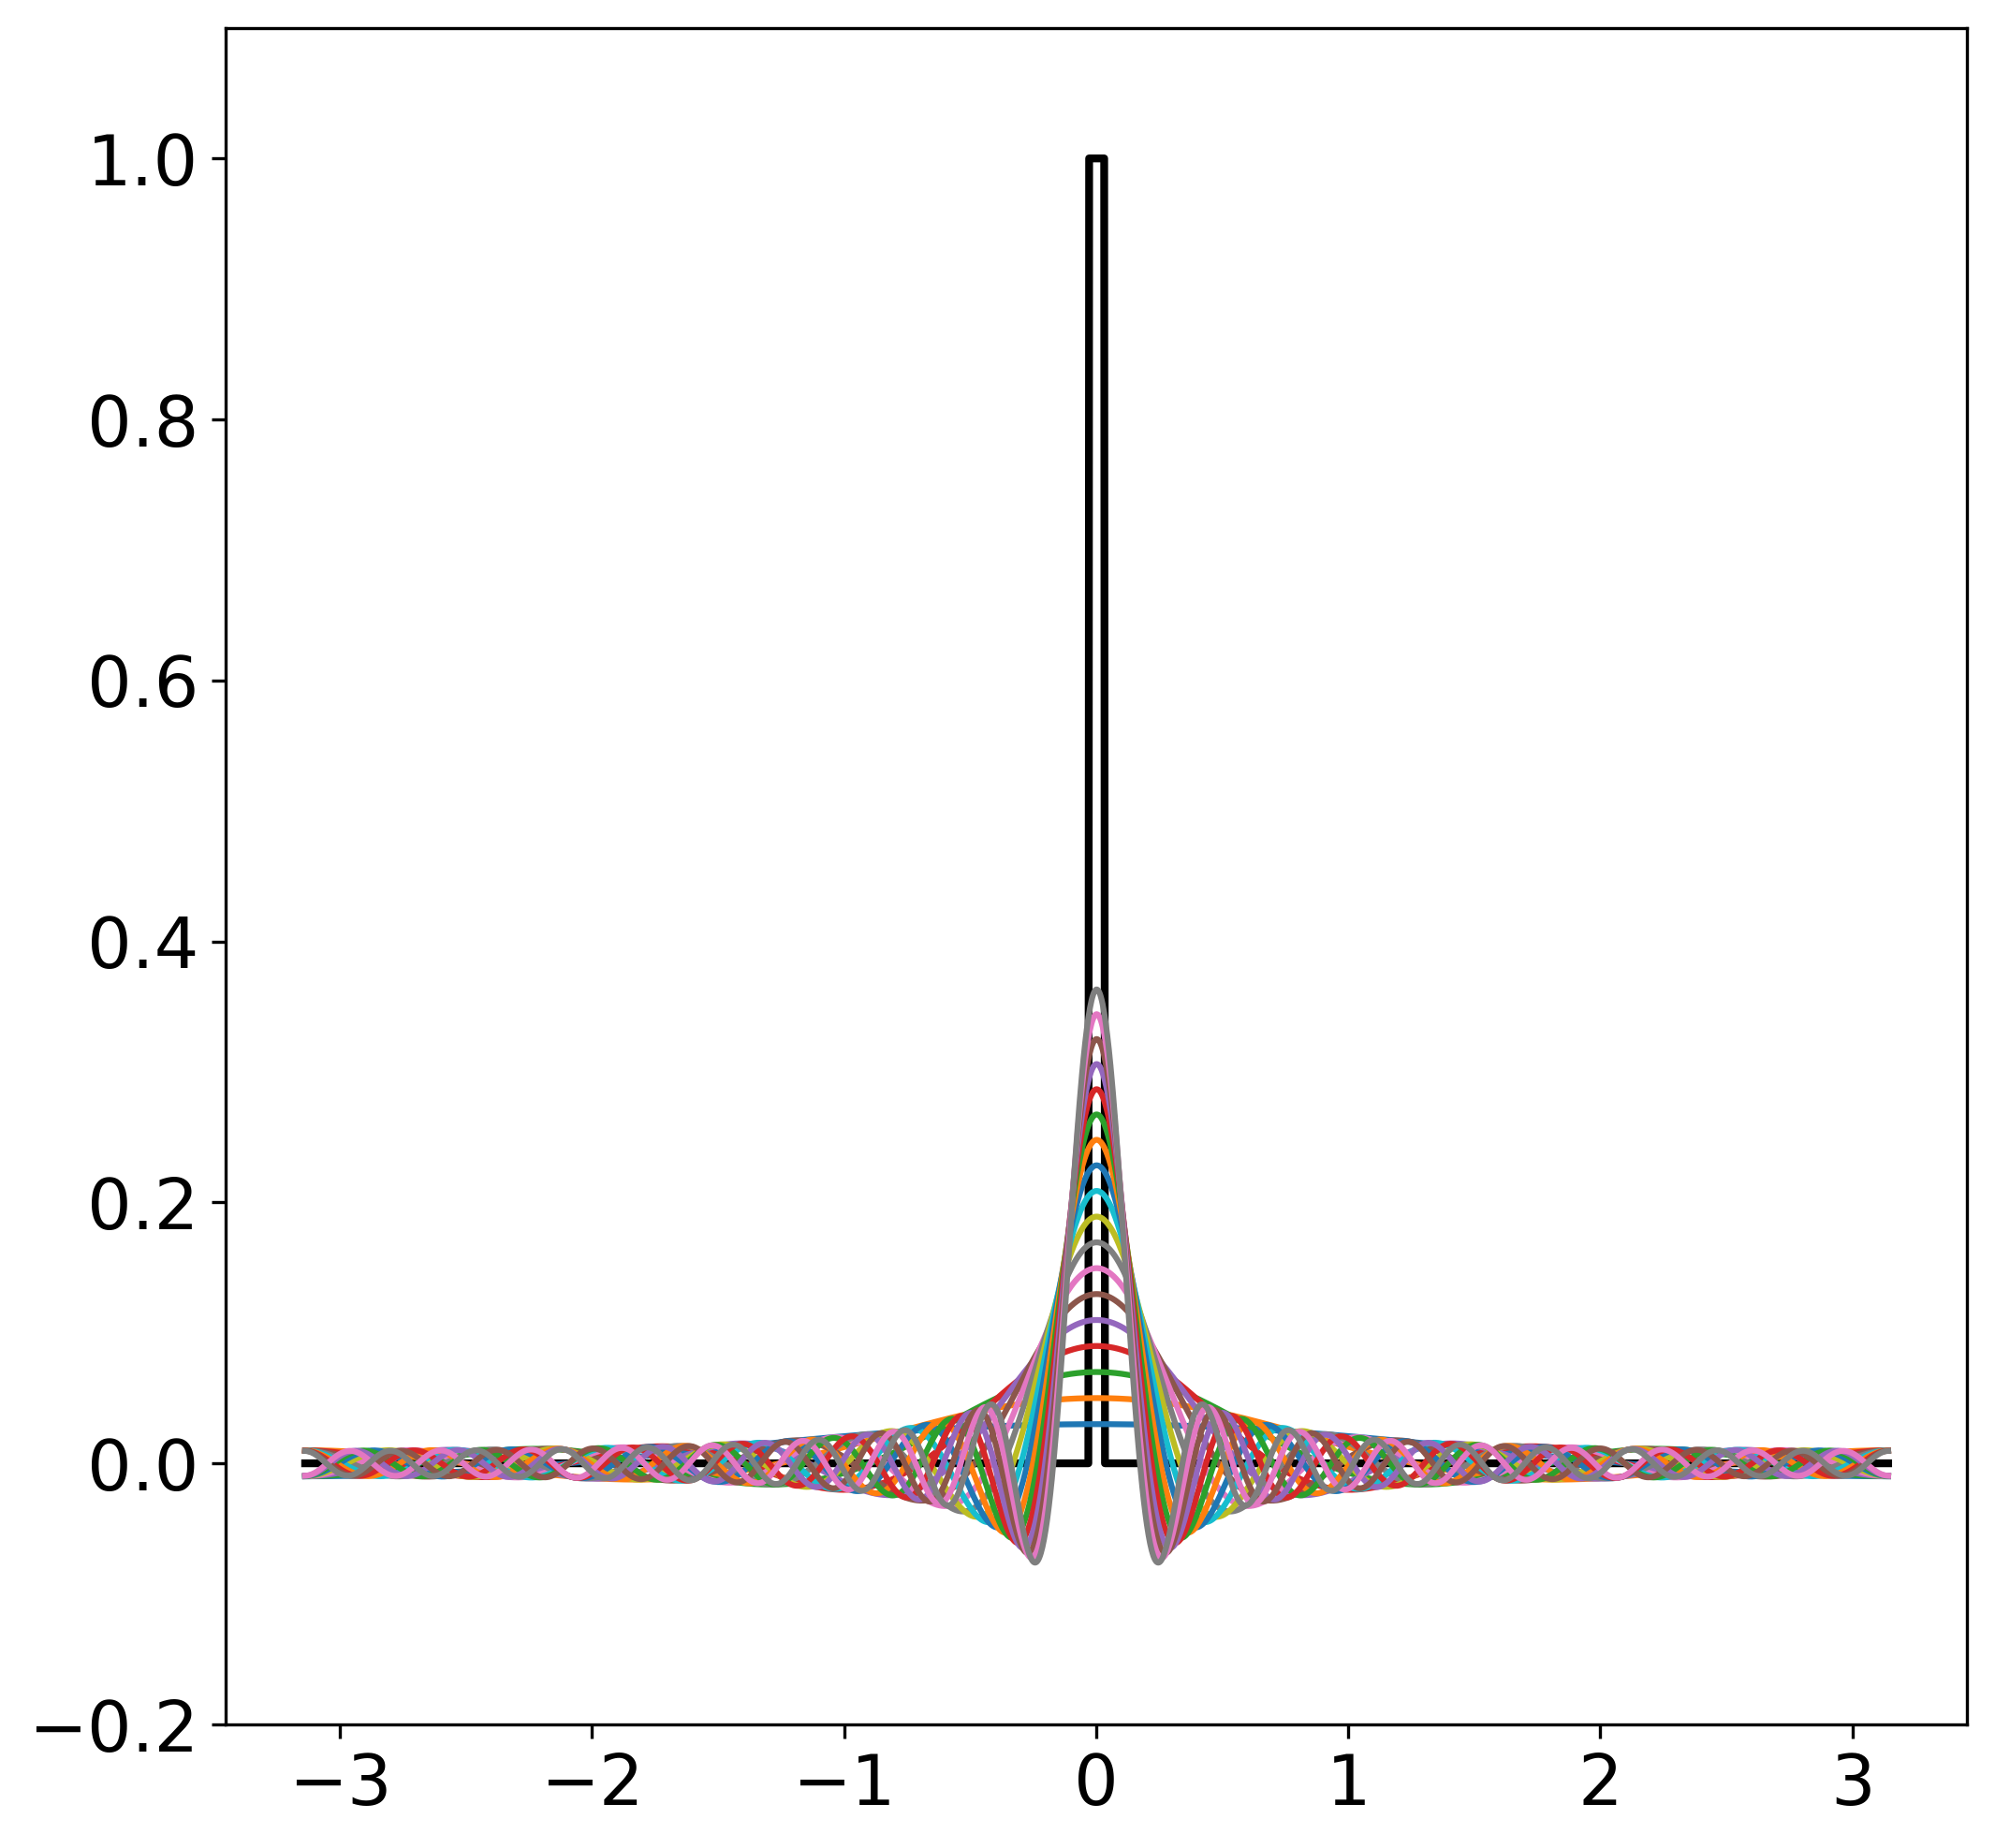
\includegraphics[width=.5\linewidth]{programs/fourier2/out_18.png}}
    \only<20|handout:0>{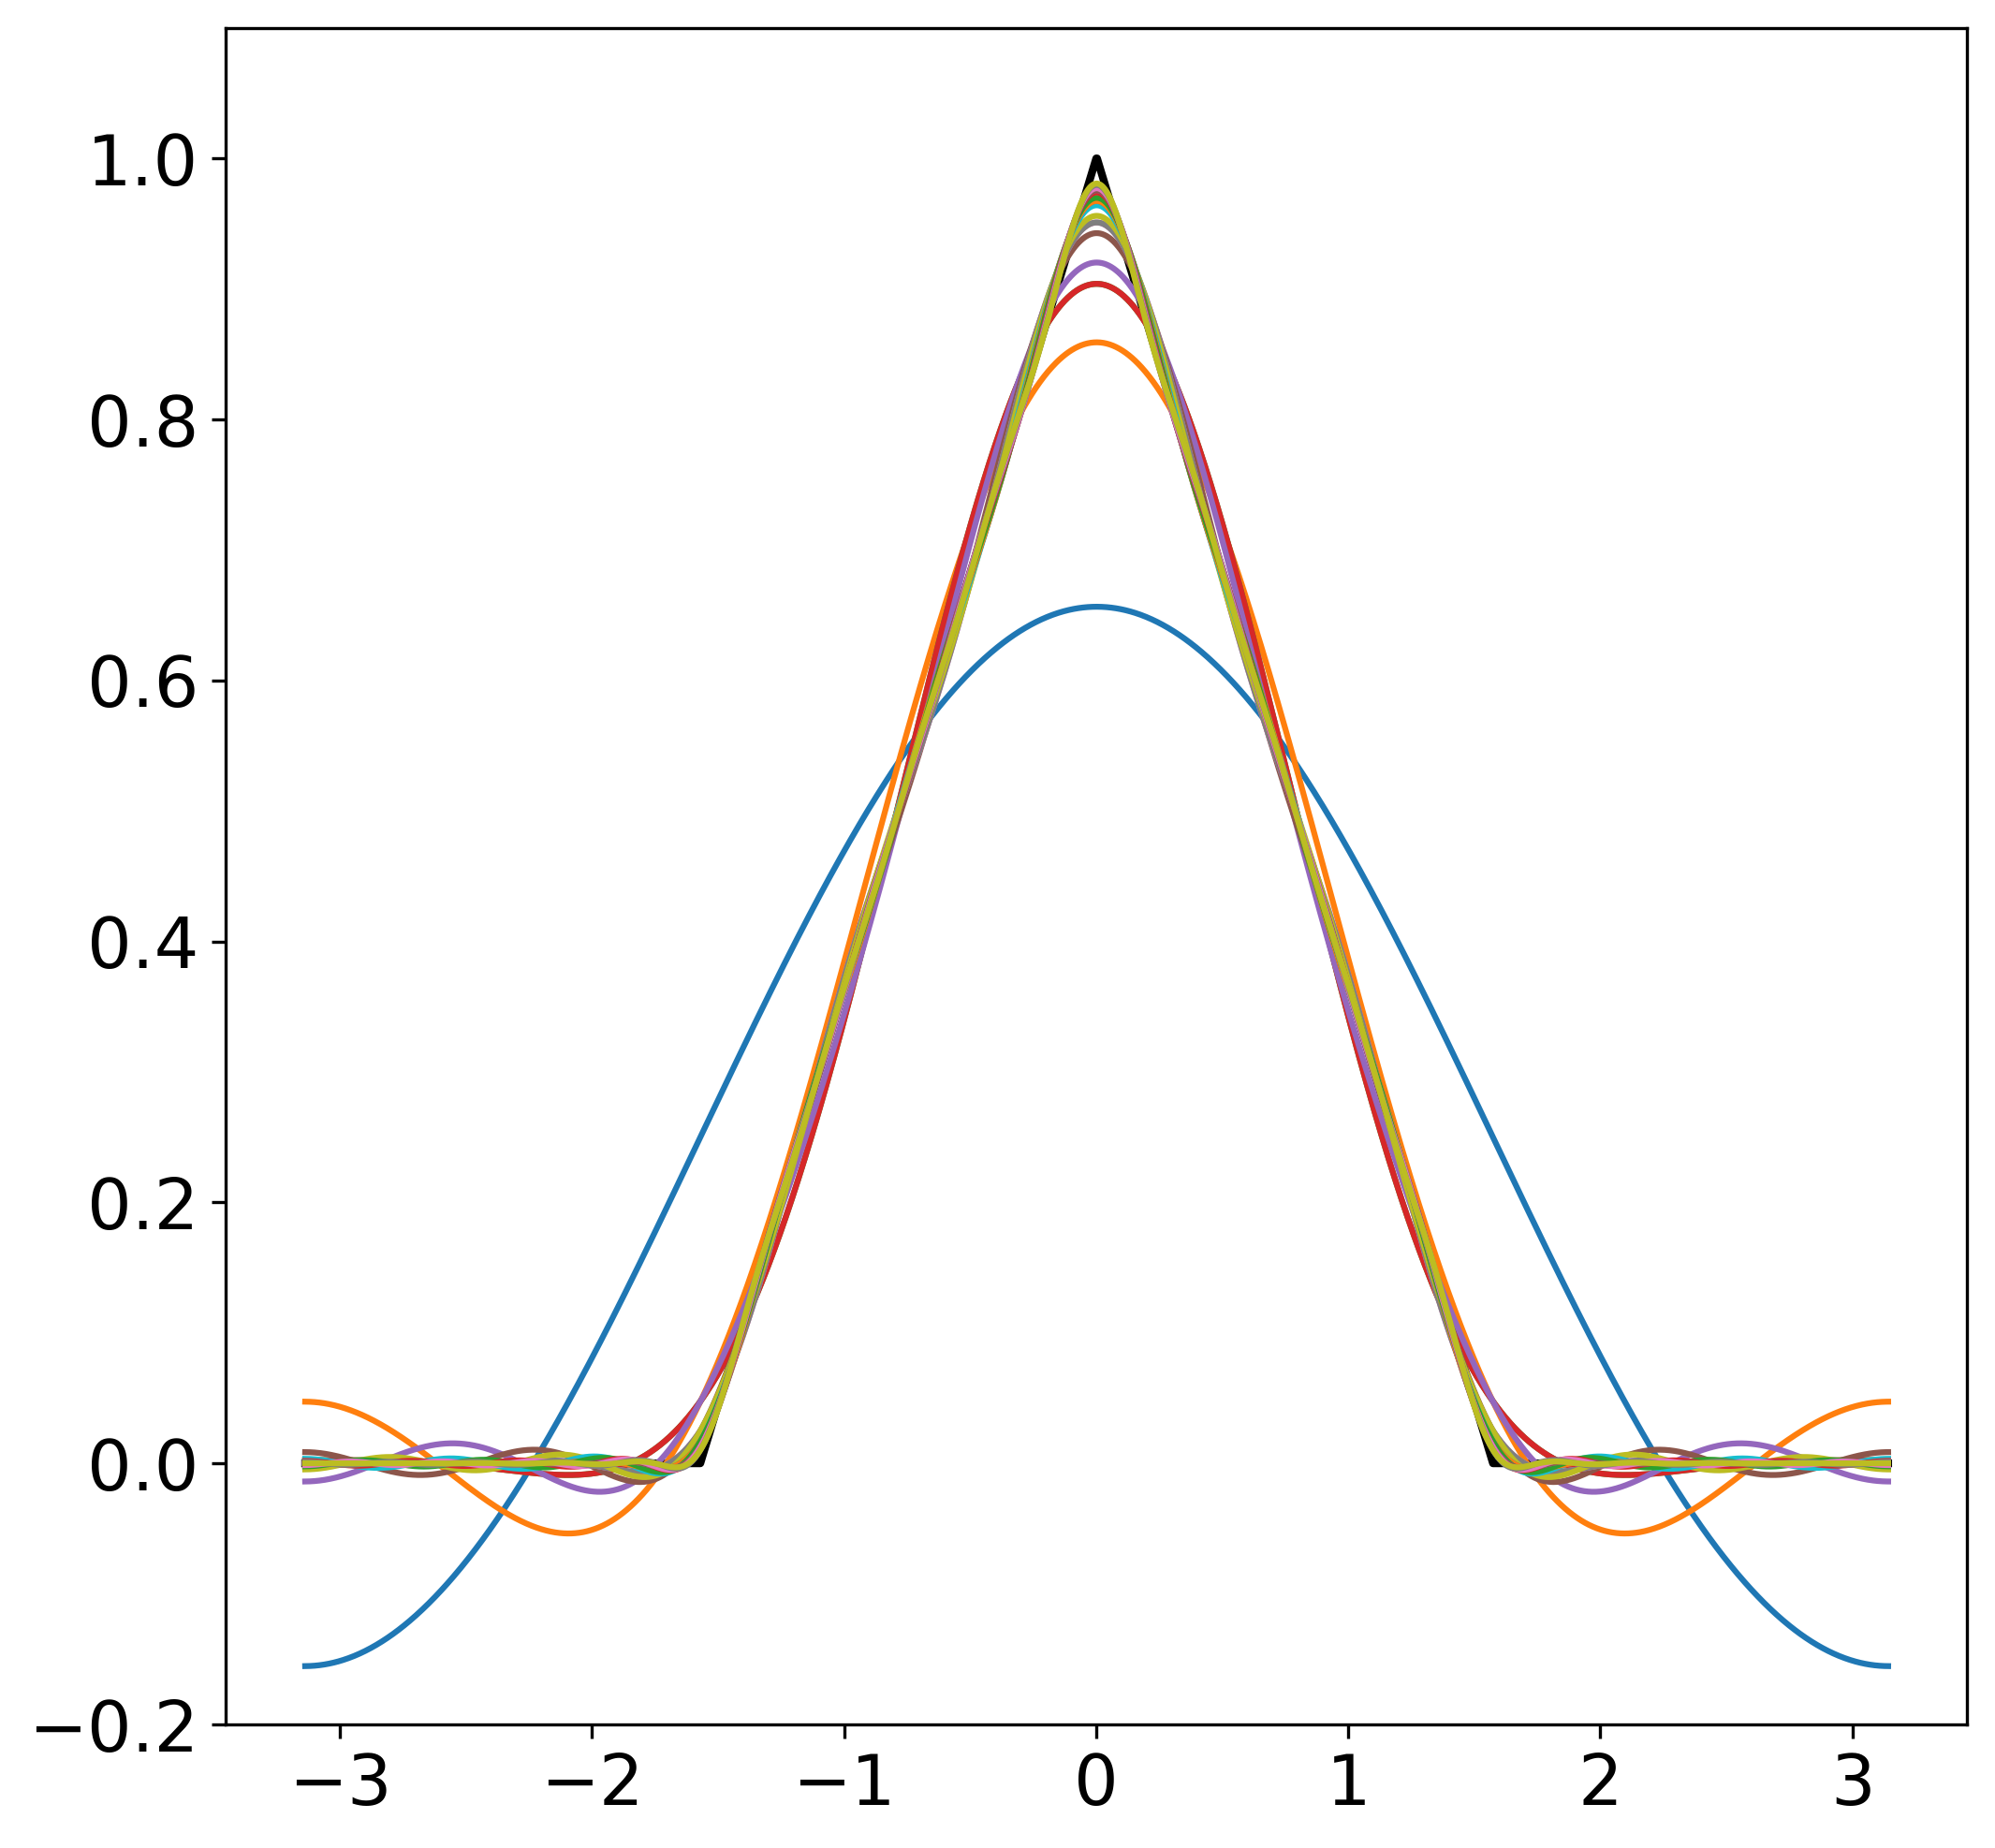
\includegraphics[width=.5\linewidth]{programs/fourier1/out_19.png}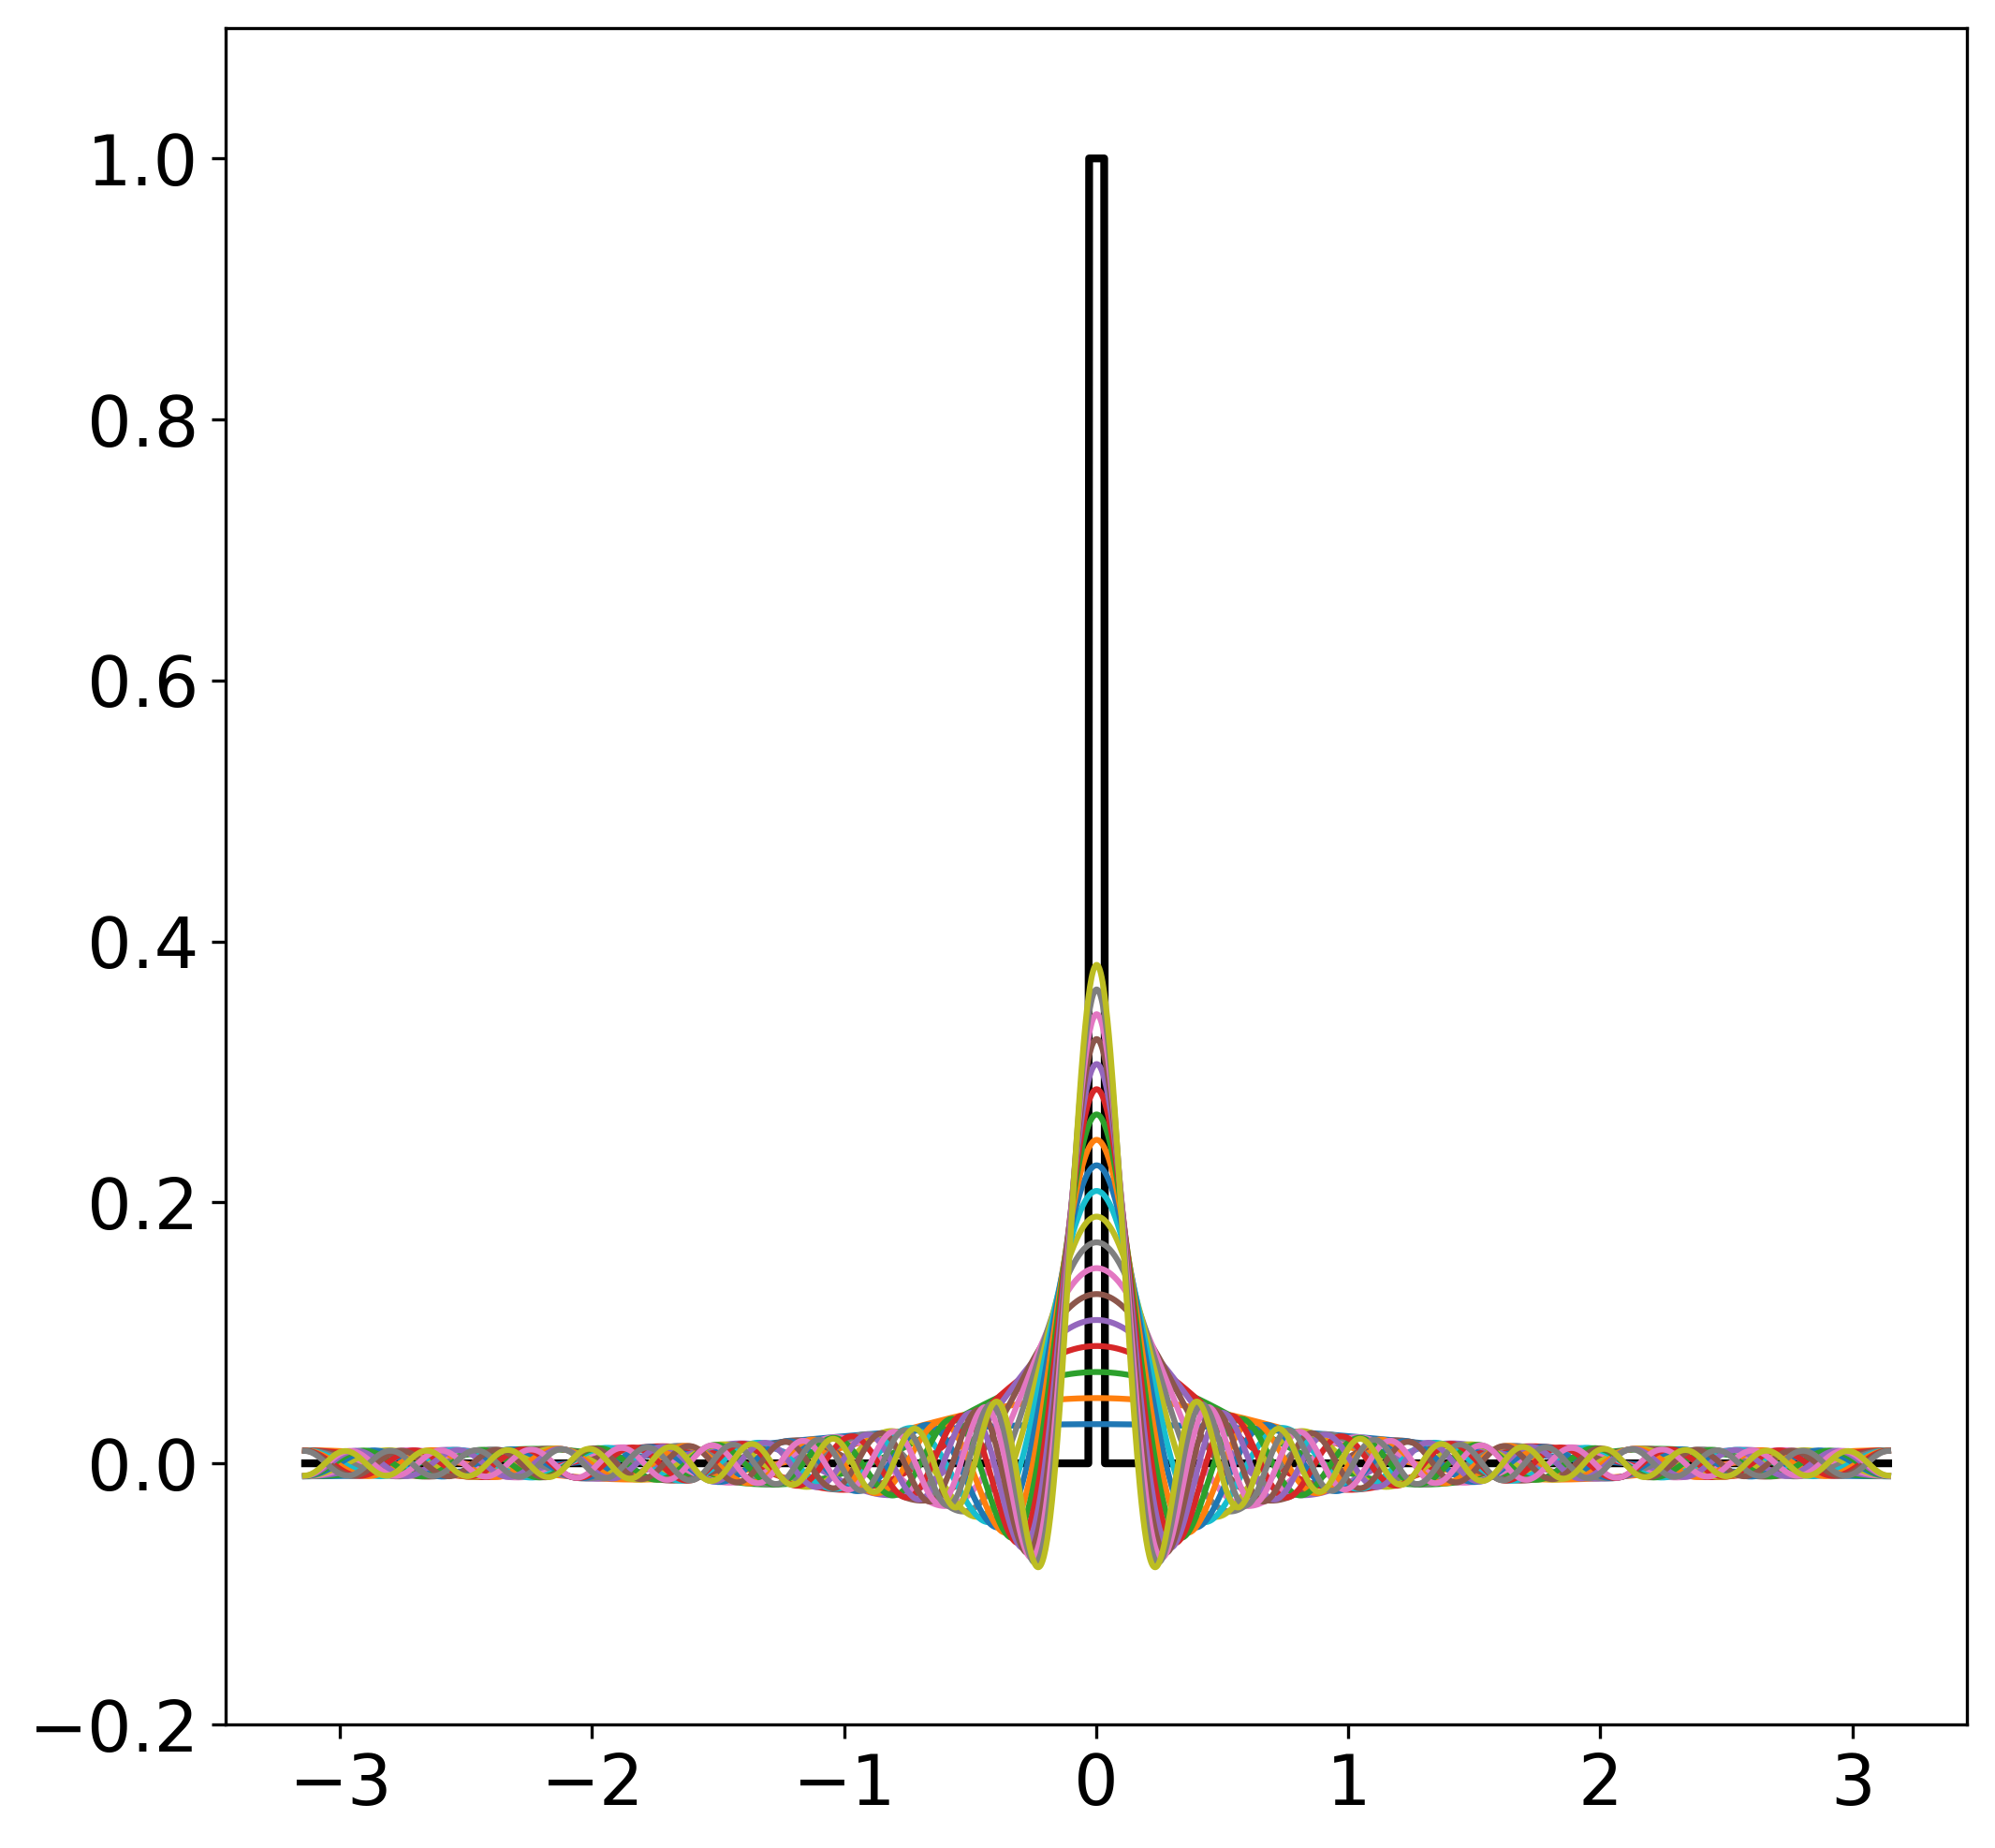
\includegraphics[width=.5\linewidth]{programs/fourier2/out_19.png}}
    \only<21>{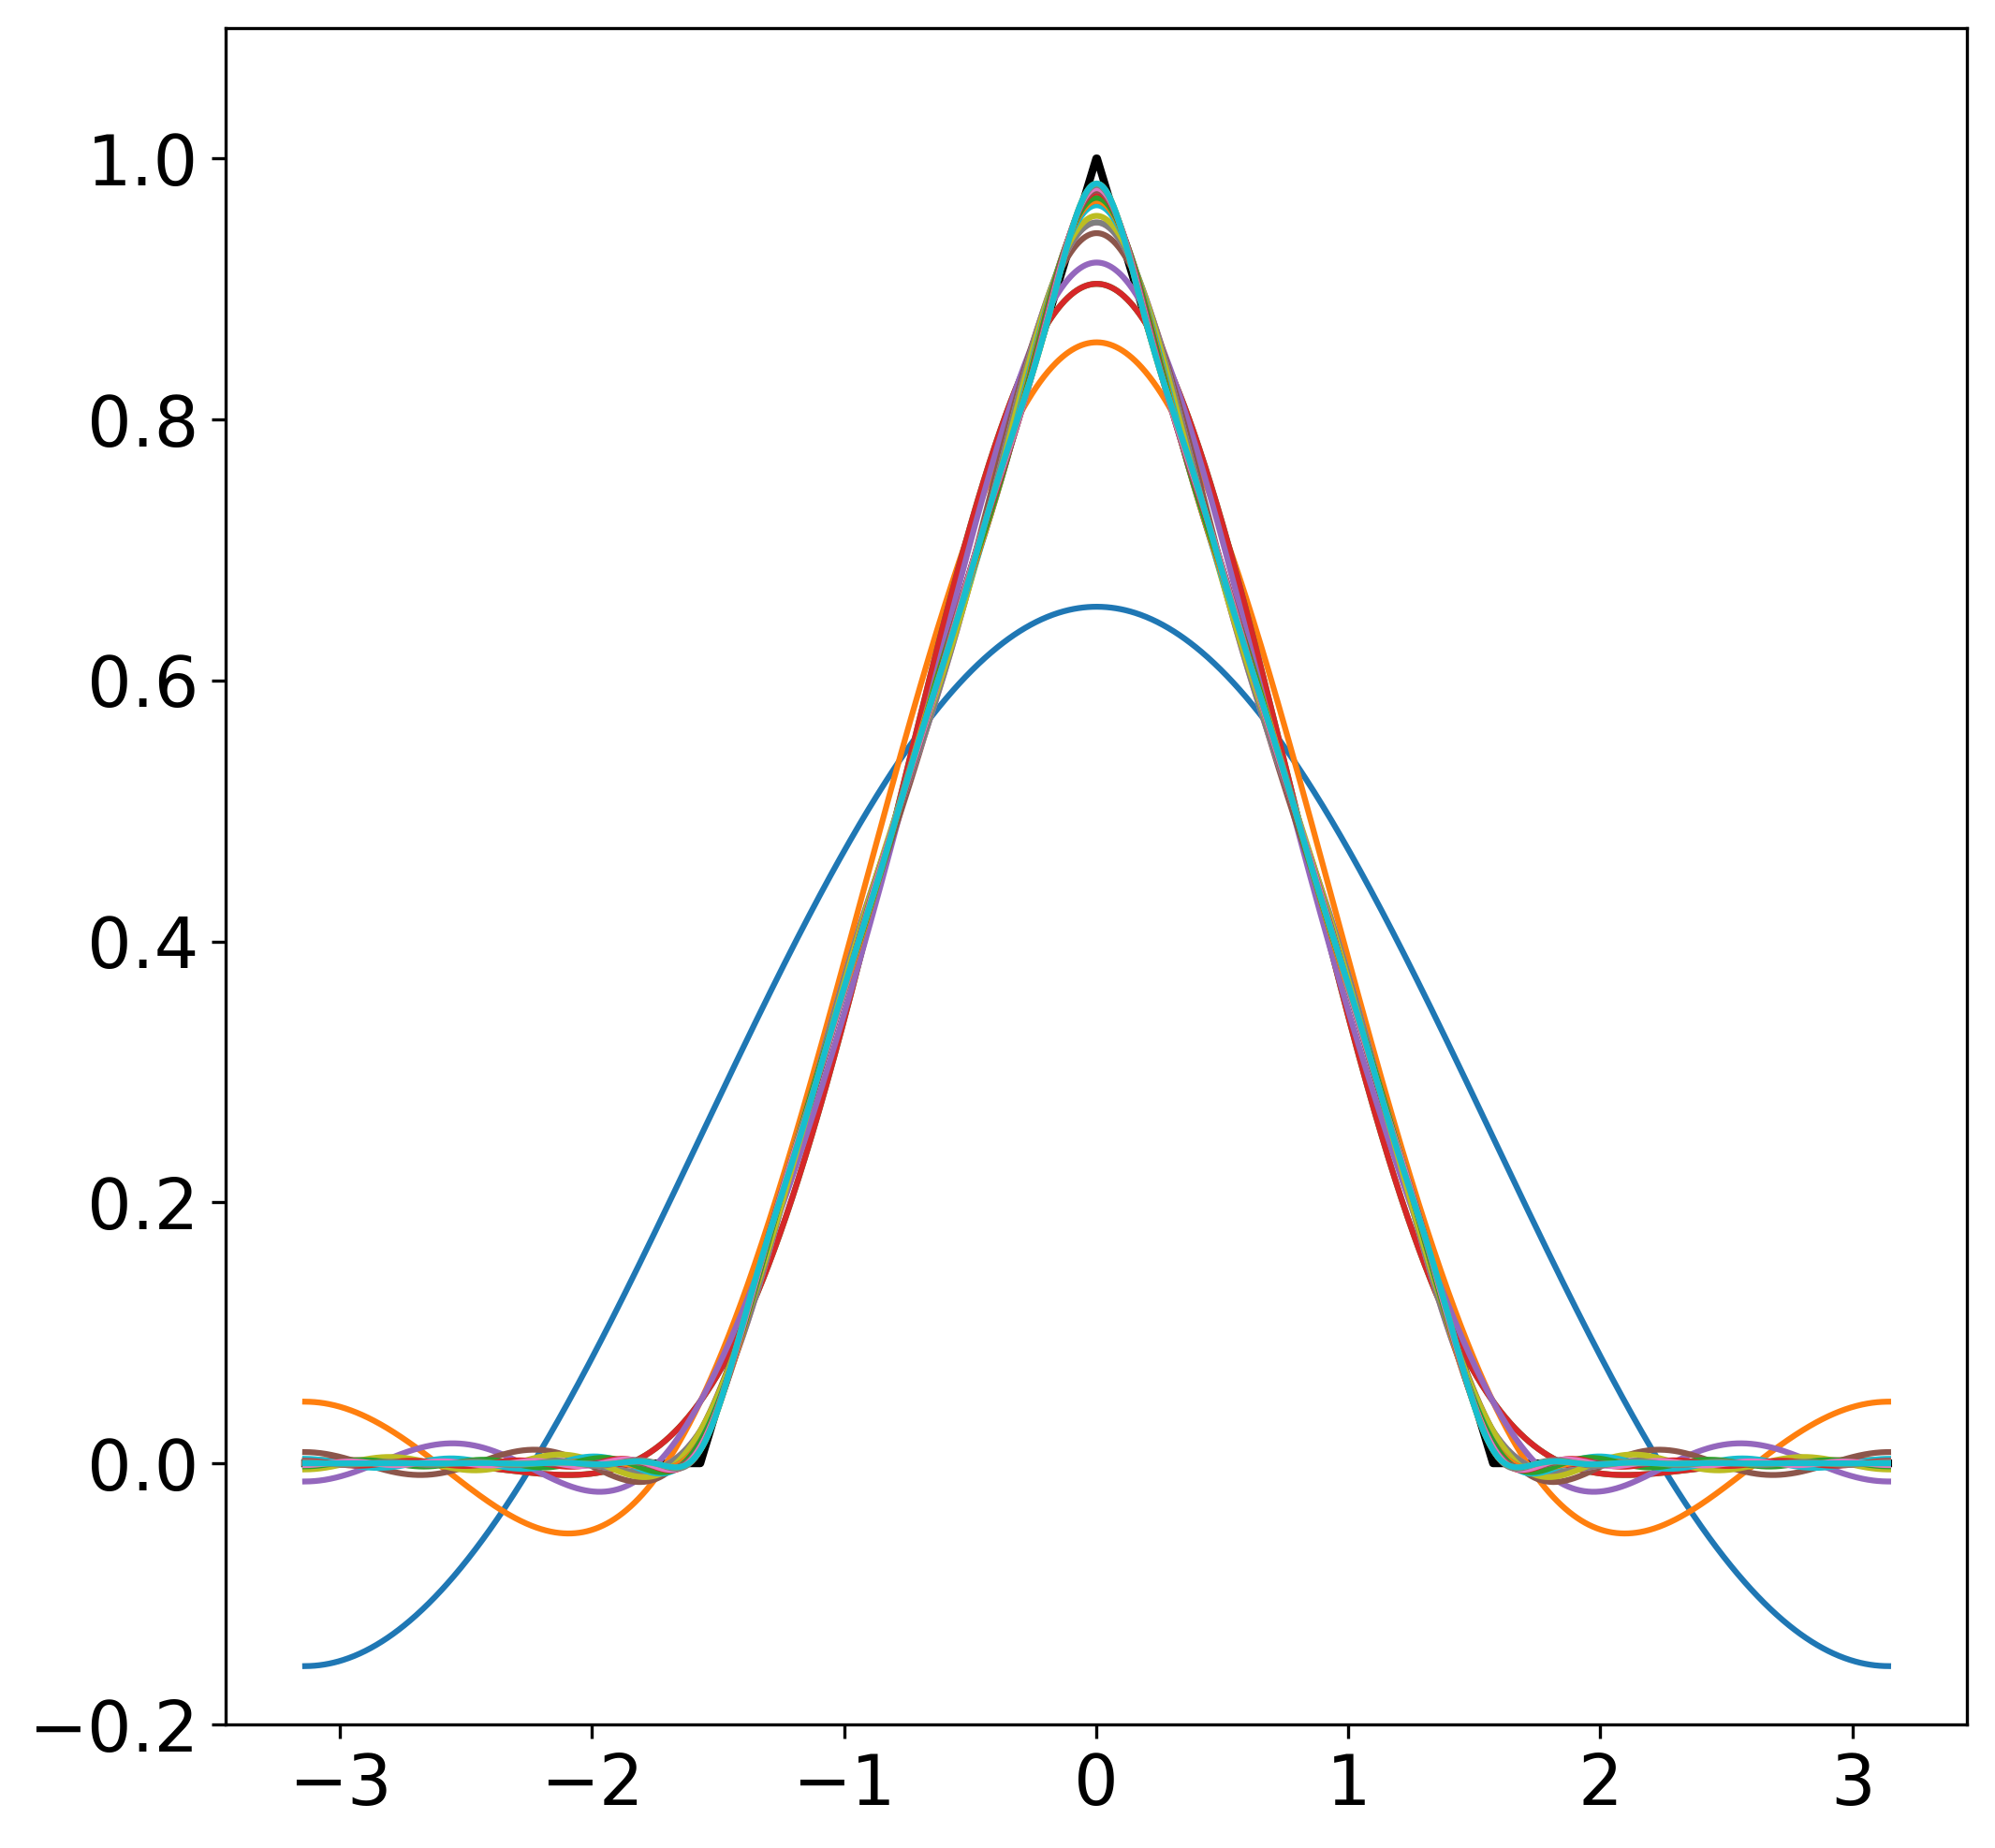
\includegraphics[width=.5\linewidth]{programs/fourier1/out_20.png}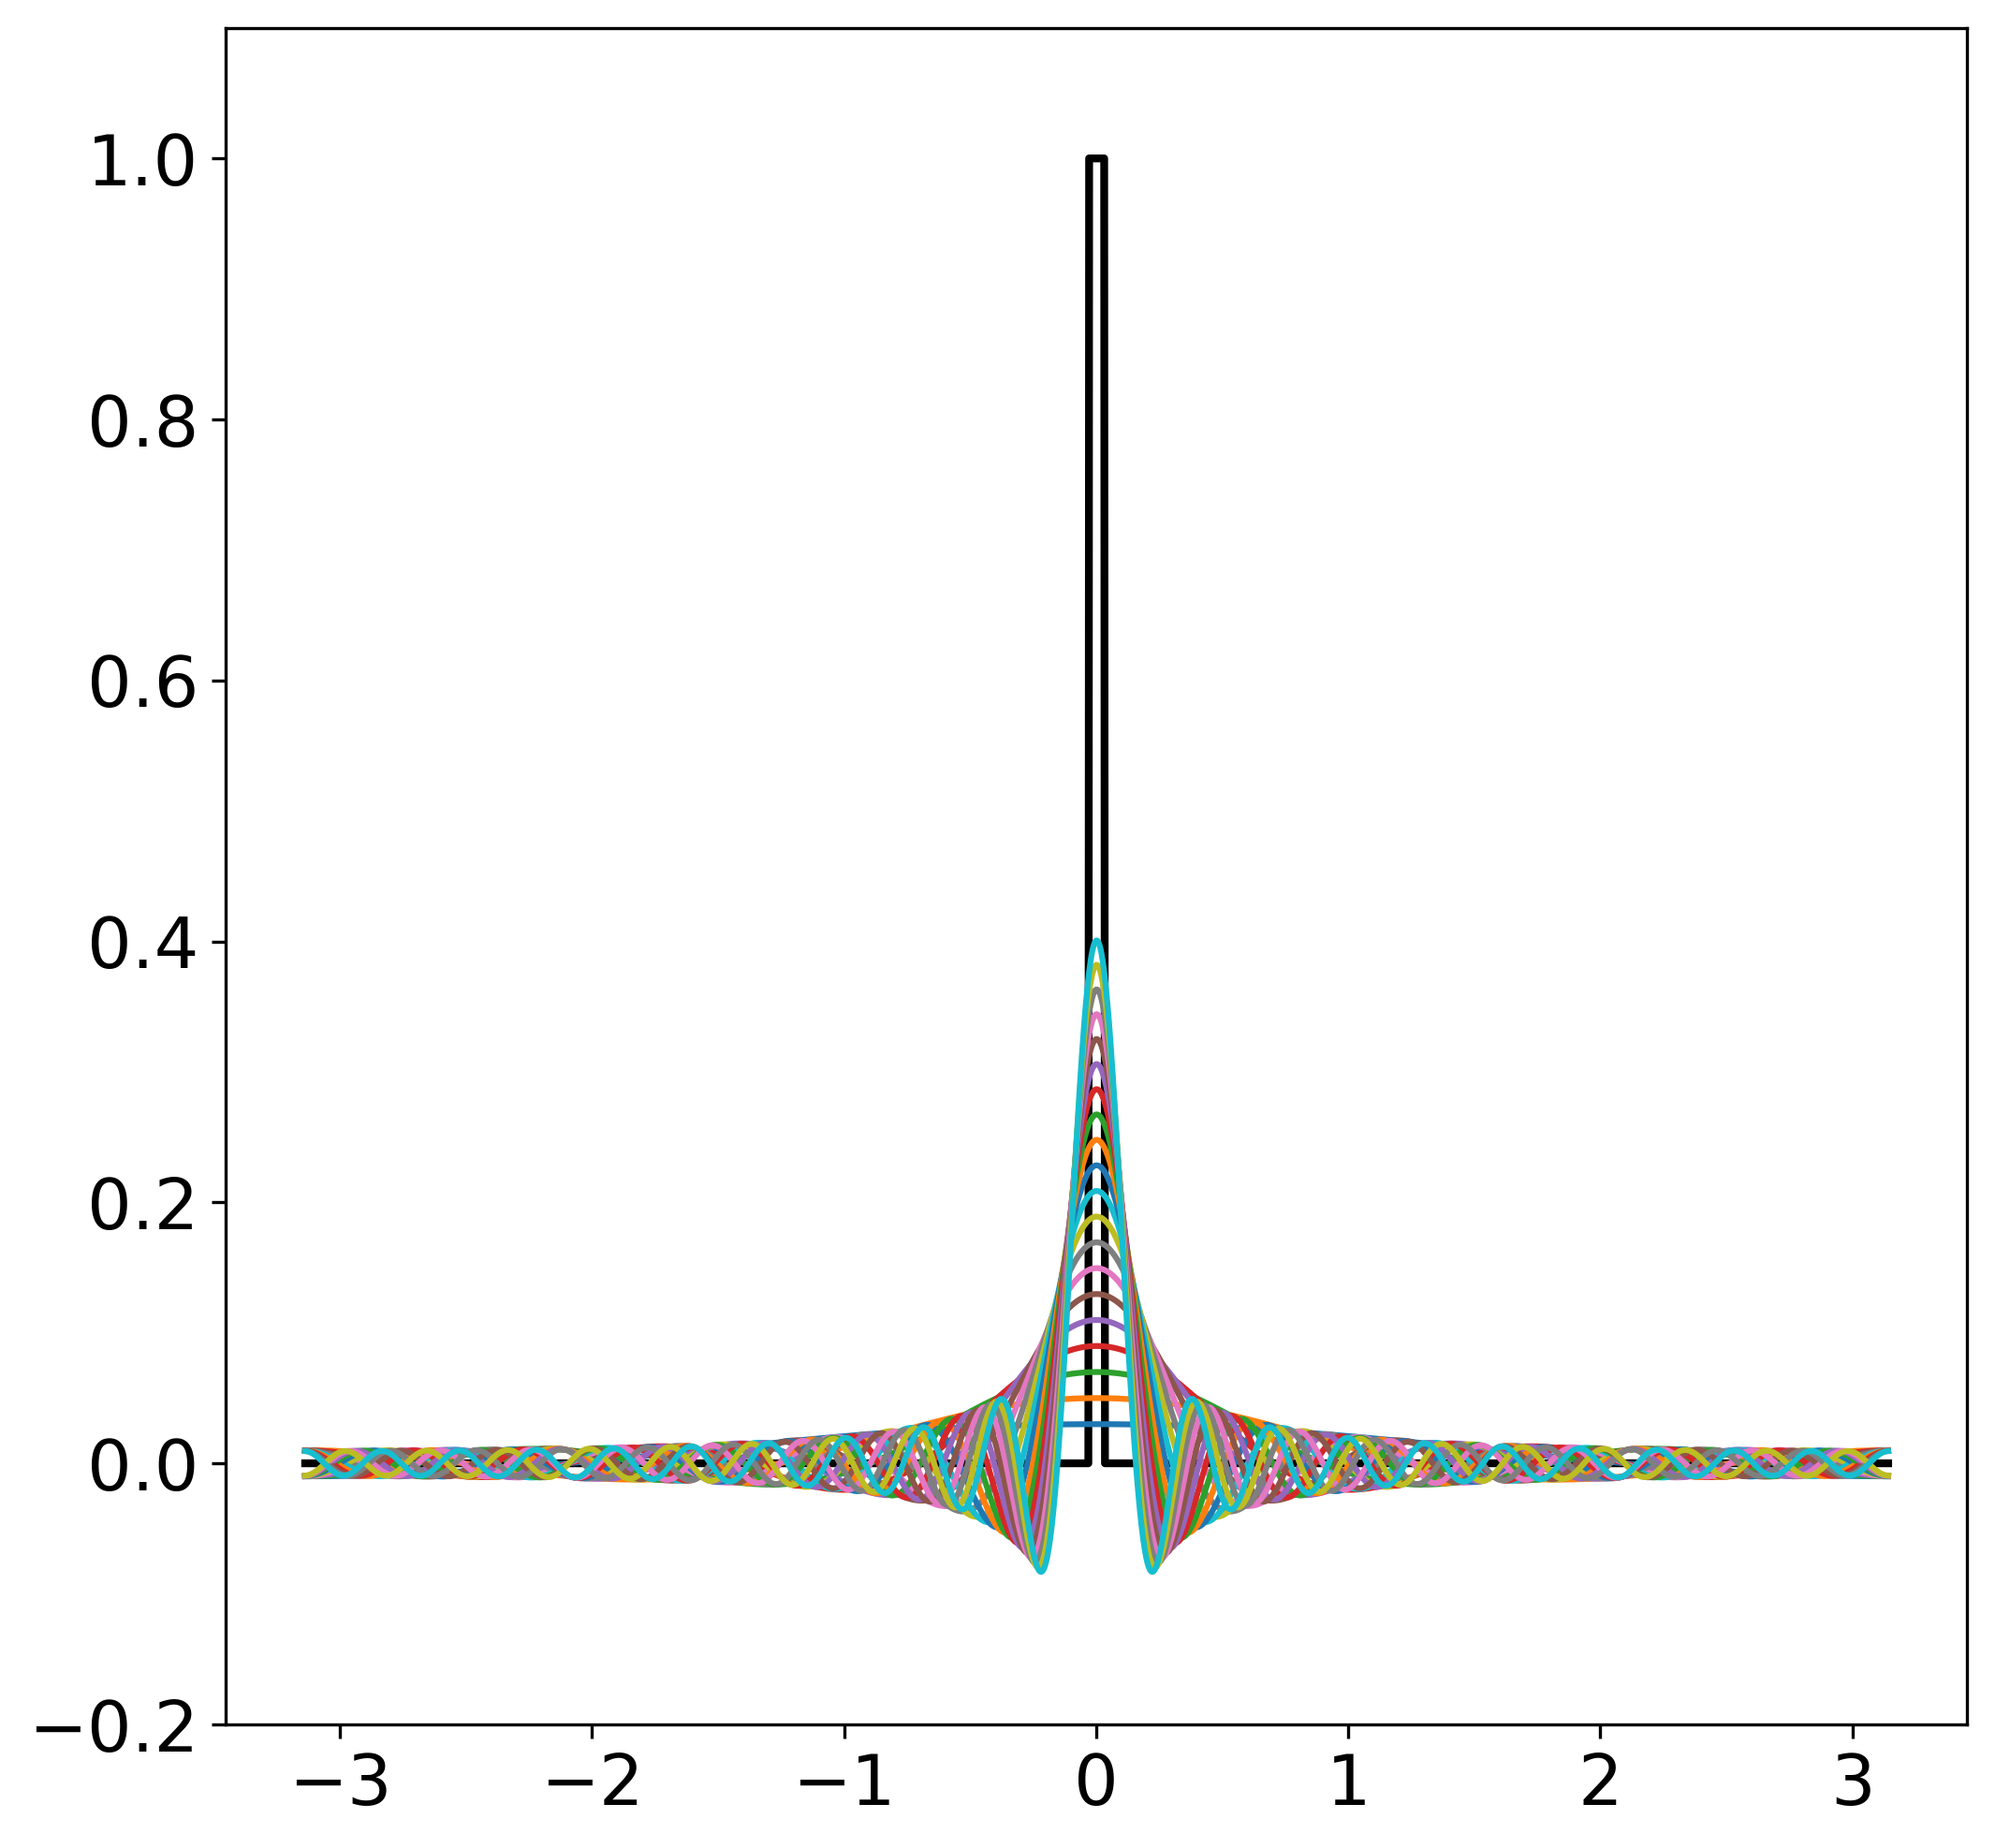
\includegraphics[width=.5\linewidth]{programs/fourier2/out_20.png}}}

  \end{frame}

  \begin{frame}
    \frametitle{Kugelflächenfunktionen (spherical harmonics)}
    \begin{itemize}[<+->]
    \item Wir betrachten die Laplace-Gleichung in Kugelkoordinaten $(r, \vartheta,\varphi)$
      $$
      \laplace \phi = 0 \text{ mit } \laplace = \underbrace{\frac{1}{r^2}\frac{\partial}{\partial r} \left( r^2 \frac{\partial}{\partial r} \right)}_{\laplace_r: \text{ Radialanteil}} + \frac{1}{r^2} \underbrace{\left( \frac{1}{\sin\vartheta} \frac{\partial}{\partial\vartheta} \sin\vartheta \frac{\partial}{\partial\vartheta} + \frac{1}{\sin^2\vartheta} \frac{\partial^2}{\partial\varphi^2}  \right)}_{\laplace_{\vartheta\varphi}: \text{ Winkelanteil}}
      $$
    \item Ansatz zur Lösung (siehe später auch \alert{Separation der Variablen})
      $$
      \phi(r,\vartheta,\varphi) = R_l(r) \cdot Y_{lm} (\vartheta,\varphi), \text{ Produktansatz}
      $$
    \item Einsetzen in Laplace-Gleichung:
      $$
      \laplace \phi = \laplace\left( R_l Y_{lm}\right) = \left(\laplace_r + \frac{1}{r^2}\laplace_{\vartheta\varphi}\right) \left( R_l Y_{lm}\right) = \boxed{Y_{lm} \laplace_r R_l + \frac{R_l}{r^2}\laplace_{\vartheta\varphi} Y_{lm} \stackrel{!}{=} 0}
      $$
    \item Umgeformt:
      $$
      \boxed{\frac{r^2\laplace_rR_l}{R_l} = - \frac{\laplace_{\vartheta\varphi} Y_{lm}}{Y_{lm}} = \text{const.} = l(l+1)}
      $$
      \end{itemize}
    \end{frame}
  
    \begin{frame}
      \frametitle{Zwei neue Differentialgleichungen}
      \begin{itemize}[<+->]
        \item Die gefundene Identität
      $$
      \boxed{\frac{r^2\laplace_rR_l}{R_l} = - \frac{\laplace_{\vartheta\varphi} Y_{lm}}{Y_{lm}} = \text{const.} = l(l+1)}
      $$
      liefert zwei neue Differentialgleichungen (eine gDGL und eine pDGL):
      \begin{align*}
      \laplace_r R_l & = \frac{l(l+1)}{r^2} R_l &\quad & \text{(Radialgleichung)} \to \Aboxed{R_l(r) = A r^l+ Br^{-(l+1)}}\\
      \laplace_{\vartheta\varphi} Y_{lm} & = - l(l+1) Y_{lm} &\quad & \text{(Winkelgleichung)}
      \end{align*}
    \item Die \alert{Winkelgleichung} ist eine \alert{Eigenwertgleichung}: Die Funktionen $Y_{lm}$ sind Eigenfunktionen zu den Eigenwerten $-l(l+1)$.
    \item Der doppelte Index \enquote{$lm$} deutet schon an, dass es zu jedem Eigenwert $-l(l+1)$ \alert{mehrere Eigenfunktionen} geben kann $\to$ \alert{Entartung}
    \item Lösungen der Winkelgleichungen existieren für $l \in \mathbb{N}_0$ und $m = -l, -l+1, \dots, l-1, l$. Diese Lösungen $Y_{lm}$ heißen \alert{Kugelflächenfunktionen}.
      \item Die Kugelflächenfunktionen $Y_{lm}$ bilden ein \alert{vollständiges Funktionensystem auf der Einheitskugel}.
        \end{itemize}
      \end{frame}

      \begin{frame}
        \frametitle{Eigenschaften der Kugelflächenfunktionen}
        \begin{itemize}[<+->]
        \item Die Kugelflächenfunktionen $Y_{lm}$ stehen in Zusammenhang mit den \alert{zugeordneten Legendrepolynomen} $P_{lm}(z)$:
          $$
          Y_{lm}\; :\; [0,\pi] \times [0,2\pi] \to \mathbb{C}, \; (\vartheta,\varphi) \to \frac{1}{\sqrt{2\pi}} \underbrace{\sqrt{\frac{2l+1}{2}\frac{(l-m)!}{(l+m)!}}}_{N_{lm}} P_{lm}(\cos\vartheta) e^{jm\varphi} 
          $$
          \item Anschauliche Erklärung und Visualisierung (Physikdidaktik WWU Münster): \url{https://youtu.be/FqAzWkwiEs8} bzw. \url{https://www.quantumvisions.net}
        \end{itemize}\pause

        \centering
        \begin{tabular}{c|c|c|c}
          $Y_{lm}$ & $l=0$& $l=1$& $l=2$ \\
          \hline
          $m=-2$  & & & $\sqrt{\frac{15}{32\pi}} \sin^2\vartheta e^{-j2\varphi}$\\
          $m=-1$  & & $\sqrt{\frac{3}{8\pi}} \sin\vartheta e^{-j\varphi}$ & $\sqrt{\frac{15}{8\pi}} \sin\vartheta\cos\vartheta e^{-j\varphi}$\\
          $m=0$  & $\sqrt{\frac{1}{4\pi}}$ & $\sqrt{\frac{3}{4\pi}} \cos\vartheta$ & $ \sqrt{\frac{5}{16\pi}} (3\cos^2\vartheta -1)$\\
          $m=+1$  & &$-\sqrt{\frac{3}{8\pi}} \sin\vartheta e^{j\varphi}$ & $- \sqrt{\frac{15}{8\pi}} \sin\vartheta\cos\vartheta e^{j\varphi}$\\
          $m=+2$  & & & $\sqrt{\frac{15}{32\pi}} \sin^2\vartheta e^{j2\varphi}$
          \end{tabular}
\end{frame}      

      \begin{frame}
        \frametitle{Eigenschaften der Kugelflächenfunktionen (...)}
        \begin{itemize}[<+->]
        \item Orthonormalität:
          $
          \int_0^{2\pi}\int_{-1}^1  Y_{l'm'}^\star(\vartheta,\varphi) Y_{lm}(\vartheta,\varphi)\upd(\cos\vartheta)\upd\varphi = \delta_{ll'}\delta_{mm'} 
          $
        \item Vollständigkeitsrelation:
          $
          \sum_{l=0}^{\infty}\sum_{m=-l}^l  Y_{lm}^\star(\vartheta',\varphi') Y_{lm}(\vartheta,\varphi) = \delta(\varphi-\varphi')\delta(\vartheta-\vartheta') 
          $
        \item Entwicklungssatz für $f=f(\vartheta,\varphi)$ quadratintegrable Funktion auf der Einheitskugel:
          \begin{align*}
            f(\vartheta,\varphi) &= \sum_{l=0}^{\infty}\sum_{m=-l}^l  c_{lm} Y_{lm}(\vartheta,\varphi) \text{ mit}\\
c_{lm} & = \int_0^{2\pi}\int_{-1}^1  Y_{lm}^\star(\vartheta,\varphi) f(\vartheta,\varphi) \upd(\cos\vartheta)\upd\varphi            
          \end{align*}
        \item Damit (und dem Produktansatz) auch Entwicklungssatz für $\phi=\phi(r, \vartheta,\varphi)$ quadratintegrable Funktion auf dem $\mathbb{R}^3$:
          \begin{align*}
            \phi(r, \vartheta,\varphi) &= \sum_{l=0}^{\infty}\sum_{m=-l}^l  \underbrace{c_{lm} R_l(r)}_{R_{lm}(r)=c_{lm}(A r^l+ B r^{-(l+1)})} Y_{lm}(\vartheta,\varphi) \text{ mit}\\
R_{lm}(r) & = \int_0^{2\pi}\int_{-1}^1  Y_{lm}^\star(\vartheta,\varphi) \phi(r,\vartheta,\varphi) \upd(\cos\vartheta)\upd\varphi            
          \end{align*}

        \end{itemize}
\end{frame}      

\begin{frame}
  \frametitle{Schlussbemerkungen}
  \begin{itemize}[<+->]
  \item Die beiden hier vorgestellten vollständigen Funktionensysteme werden nicht die einzigen bleiben.
  \item Bei kartesischen Symmetrien: häufig \alert{harmonische Funktionen} (Fourier) eine gute Wahl
  \item Bei sphärischer Symmetrie: häufig \alert{sphärisch harmonische Funktionen} (Kugelflächenfunktionen) eine gute Wahl
  \item Bei zylindrischer Symmetrie: häufig \alert{Bessel-Funktionen} eine gute Wahl
    \item Wir werden das wieder aufgreifen, wenn entsprechende Probleme betrachtet werden.
    \end{itemize}
\end{frame}


\input{finalframe.inc}
   
\end{document}